% An MSI thesis template thrown together Oct 2005 - CW



\documentclass[a4paper,12pt]{book}
\usepackage{mathtools}
\usepackage{subcaption}
\usepackage{enumerate}
\usepackage{lscape}
\usepackage{graphicx,psfrag}
\usepackage{pgfplotstable}
\usepackage{adjustbox}
\usepackage{tikz}
\usepackage{hyperref}
\usepackage[numbers]{natbib} 
\bibliographystyle{unsrtnat}
%\pgfplotsset{compat=1.13}

  % a file containing your definitions, which packages to load etc
    \usepackage{amssymb}
  \usepackage{latexsym}
  \usepackage{amsfonts}
  \usepackage{amsthm}
  \usepackage{amsmath}
  \usepackage{tikz}


% put your command and environment definitions here



% some theorem environments
% remove "[theorem]" if you do not want them to use the same number sequence


  \newtheorem{theorem}{Theorem}[chapter]
  \newtheorem{lemma}[theorem]{Lemma}
  \newtheorem{prop}[theorem]{Proposition}
  \newtheorem{cor}[theorem]{Corollary}

  \newtheorem{conj}{Conjecture}
  \renewcommand{\theconj}{\Alph{conj}}  % numbered A, B, C etc
  
  \newcommand{\matr}[1]{\mathbf{#1}}
  \newcommand{\vecn}[1]{\boldsymbol{#1}}
  \newcommand\solidrule[1][0.25cm]{\rule[0.5ex]{#1}{1.5pt}}
  \newcommand\dashedrule{\mbox{%
  		\solidrule[2mm]\hspace{2mm}\solidrule[2mm]}}
  \DeclareRobustCommand{\squaret}[1]{\tikz{\draw[#1] (0,0) rectangle (0.2cm,0.2cm);}}
  \DeclareRobustCommand{\circlet}[1]{\tikz{\draw[#1] (0,0) circle [radius=0.1cm];}}
  \DeclareRobustCommand{\trianglet}[1]{\tikz{\draw[#1] (0,0) --
  		(0.25cm,0) -- (0.125cm,0.25cm) -- (0,0);}}
  \DeclareRobustCommand{\diamondt}[1]{\tikz{\draw[#1] (0,0) --(0.1cm,0.15cm) -- (0.2cm,0cm) -- (0.1cm,-0.15cm) -- (0,0)  ;}}
  \DeclareRobustCommand{\squareF}[1]{\tikz{\filldraw[#1,fill opacity= 0.3] (0,0) rectangle (0.2cm,0.2cm);}}
 
  
  \newcommand{\dotrule}[1][4mm]{%
  	\parbox{#1}{\dotfill}} 

  \theoremstyle{definition}
  \newtheorem{defn}[theorem]{Definition}
  \newtheorem{ex}[theorem]{Example}
  \newtheorem{exs}[theorem]{Examples}
  \newtheorem{question}[theorem]{Question}
  \newtheorem{remark}[theorem]{Remark}
  \newtheorem{notn}[theorem]{Notation}
  \newtheorem{alg}[theorem]{Algorithm}


  % line-spacing factor
  \renewcommand{\baselinestretch}{1.2}

  % use this if you don't want headers and page numbers on
  % blank pages at the end of chapters
  \newcommand{\blanknonumber}{\newpage\thispagestyle{empty}}

  % needed for ANU logo on titlepage (optional)
  \usepackage{graphics}

  % margins
  \setlength{\voffset}{-1in}
  \setlength{\hoffset}{-1in}
  \setlength{\oddsidemargin}{4cm}
  \setlength{\evensidemargin}{2.5cm}
  \setlength{\textwidth}{14.5cm}
  \setlength{\textheight}{22.5cm}
  \setlength{\topmargin}{2.5cm}


  % for working drafts, un-comment the following command and list
  % the chapters etc you want to see in the output, eg
  %\includeonly{chp3/chapter}



\begin{document}


  % set page numbers to roman and suppress chapter numbers
  \frontmatter


  % remove or switch the order of these as you see fit
 \begin{titlepage}
\begin{center}

\vspace*{\fill} \Huge
                        Simulation of Rapidly Varying and Dry Bed Flow 
                        using the Serre equations solved by a Finite Element Volume Method.
\\
\vfill\vfill\Large
                          Jordan Peter Anthony Pitt
\\
\vfill\vfill
                          January 2019
\\
\vfill\vfill \normalsize
         A thesis submitted for the degree of Doctor of Philosophy\\
         of the Australian National University
\vfill
        %
\includegraphics{ANU.eps}
         \anulogo

\end{center}

\end{titlepage}
\blanknonumber
  %

\blanknonumber\ \blanknonumber

\vspace*{\fill}

\begin{center}\emph{
%
To my mother and father who have provided me with everything.
%
}
\end{center}

\vfill\vfill\vfill
\blanknonumber
  %
\chapter*{Declaration}\label{declaration}
\thispagestyle{empty}
The work in this thesis is my own except where otherwise stated.

\vspace{1in}


\hfill\hfill\hfill
%
Jordan Pitt
%
\hspace*{\fill}
\blanknonumber
  %
\chapter*{Acknowledgements}\label{acknowledgements}
\addcontentsline{toc}{chapter}{Acknowledgements}


% your acknowledgements go here

%Beji
%Chris
%Stephen Roberts

I would like to thank my lead supervisor Professor Stephen Roberts for his insight, suggestions and time spent improving my research. Dr Chris Zoppou who put a tremendous amount of time and effort into reading and editing my work. The remainder of my supervisor panel Professor Markus Hegland and Professor John Urbas.


I would also like to thank our fellow researchers who provided us with experimental data:
\begin{itemize}
	\item Dr David George, Cascades Volcano Observatory, U.S. Geological Survey for providing the digitised data for the rectangular depression experiment.
	\item Professor Sedar Beji, Department of Naval Architecture and Ocean Engineering, Istanbul Technical University, for providing the data for the periodic waves over a submerged bar experiment.
	\item Dr Volker Roeber, Department of Physical Oceanography, University of Hawai`i at M\={a}noa for providing the data for the solitary wave over a fringing reef experiment.  
\end{itemize}
\blanknonumber
  %\chapter*{Abstract}\label{abstract}

\addcontentsline{toc}{chapter}{Abstract}

112233
\blanknonumber
 \tableofcontents\blanknonumber
  %

\chapter{Notation and terminology}\label{notation}
%\addcontentsline{toc}{chapter}{Notation and terminology}

\renewcommand{\thefootnote}{\fnsymbol{footnote}}


%
%Some preliminary description here?  Eg, ``In the following, $G$ is
%a group, $H$ is a subgroup of $G$, \ldots''
%\\
%
%
%\

\noindent\textbf{Notation}

% adjust the lengths to suit your needs (difference of .22cm works best)

\newcommand{\nttn}[2]{\item[{\ \makebox[3.18cm][l]{#1}}]{#2}}
\begin{list}{}{ \setlength{\leftmargin}{3.4cm}
                \setlength{\labelwidth}{3.4cm}}

\nttn{$\omega^\pm$}{The angular frequency of a wave, distinguished by $\pm$ for the positive and negative branches respectively}

\nttn{$k$}{angular wave number of a wave.}

\nttn{$\lambda$}{the wavelength of a wave}

\end{list}

\

%\noindent\textbf{Terminology}
%
%% adjust the lengths to suit your needs (difference of .22cm works best)
%
%\newcommand{\term}[2]{\item[{\ \makebox[4.58cm][l]{#1}}]{#2}}
%\begin{list}{}{ \setlength{\leftmargin}{4.8cm}
%                \setlength{\labelwidth}{4.8cm}}
%
%\term{terminology}{definition text goes here definition text goes
%                   here definition text goes here}
%
%\term{terminology}{definition text goes here definition text goes
%                   here definition text goes here}
%
%\term{terminology}{definition text goes here definition text goes
%                   here definition text goes here}
%
%\end{list}
\blanknonumber



  % set page numbers to arabic, reset to 1
  \mainmatter

  % assuming there are files chapter1.tex etc...
 
\chapter{Experimental Validation}
\label{chp:ExpMethodComp}
In this chapter the second-order hybrid finite volume methods are assessed using experimental data. 

The numerical methods $\text{FDVM}_2$ and $\text{FEVM}_2$ are experimentally validated by comparing their numerical solutions to experimental data. The chosen experiments allow the methods capability to model a variety of physical situations to be tested. These situations include the presence of steep gradients in the flow, the interaction of strong dispersive waves with varying bathymetry, shoaling and wave breaking and finally the wetting and drying of a beach. Thus, the ability of these methods to reproduce all the experimental results well strongly demonstrates their capability to model all physical situations very well. 

\section{Evolution of Rectangular Depression}
A series of experiments studying the evolution of rectangular depressions and thus steep gradients in the free-surface was conducted by \citet{Hammack-Segur-1978-337}. These experiments were performed in a wave tank that was $0.394m$ wide, $31.6m$ long and $0.61m$ high. The rectangular depressions were generated using a piston $0.61m$ long with its left edge against the wave tank wall. The $0.1m$ deep water is initially stationary with a horizontal free surface and the piston in the up position. The experiment begins when the piston suddenly moves down. This creates a sudden depression in the water surface, generating waves that are recorded at wave gauges located at $0m$, $5m$, $10m$, $15m$ and $20m$ from the right edge of the piston. A diagram of the longitudinal section of the wave-tank with the wave gauge locations is given in Figure \ref{fig:SegurWT}.

\begin{figure}
	\centering
	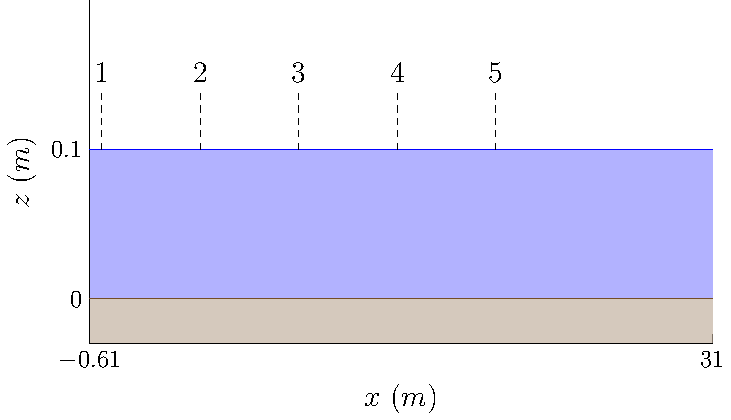
\includegraphics[width=\textwidth]{./chp6/figures/Experiment/Segur/WaveTank.pdf}
	\caption{Diagram demonstrating the water (\squareF{blue}) and the bed (\squareF{brown!80!black}) for the Segur experiments, with the wave gauge locations marked.}
	\label{fig:SegurWT}
\end{figure} 

These experiments provide a good benchmark for the capability of the numerical method to accurately model problems with steep gradients in the free surface. These experiments are affected by bed friction and viscosity and the inability of the piston and water to move vertically instantaneously. Since the Serre equations do not contain viscosity, bed friction and we use discontinuous initial conditions we expect numerical solutions of the Serre equations to produce many more oscillations in  the dispersive wave trains than are observed experimentally \cite{Pitt-2018-61}.

\citet{Hammack-Segur-1978-337} report the results for two different initial depression depths $0.01m$ and $0.03m$, resulting in the nonlinearity parameters $\epsilon = 0.1$ and $\epsilon=0.3$ respectively. Since these nonlinearity parameters are relatively small there was no breaking of waves throughout the experiment. 

This experiment was modelled numerically using the reflected problem, with the wall as the axis of symmetry. In the numerical experiments the domain is $[-60m,60m]$ and the experiment is run for $ 50s$ with $g = 9.81m/s^2$. For the spatial resolution we set $\Delta x = 0.01m$ to satisfy the CFL condition, \eqref{eqn:CFLcond} $\Delta t = 0.5 \Delta x / \sqrt{g \; 0.1}$. The limiting parameter $\theta = 1.2$ was used in the reconstruction in $\text{FEVM}_2$ and $\text{FDVM}_2$.

\subsection{Results for $0.01m$ Rectangular Depression}

Plots comparing the numerical and experimental wave gauge data for the $0.01m$ rectangular depression are displayed in Figures \ref{fig:Segur1cmFEVM} and \ref{fig:Segur1cmFDVM} for $\text{FEVM}_2$ and $\text{FDVM}_2$ respectively. We present this data using the same dimensionless scales as reported in the original paper \cite{Hammack-Segur-1978-337}. Tables \ref{tab:ConservationSegurFEVM1cm} and \ref{tab:ConservationSegurFDVM1cm} are also provided, which record the conservation of all the quantities. 
\begin{figure}
	\centering
	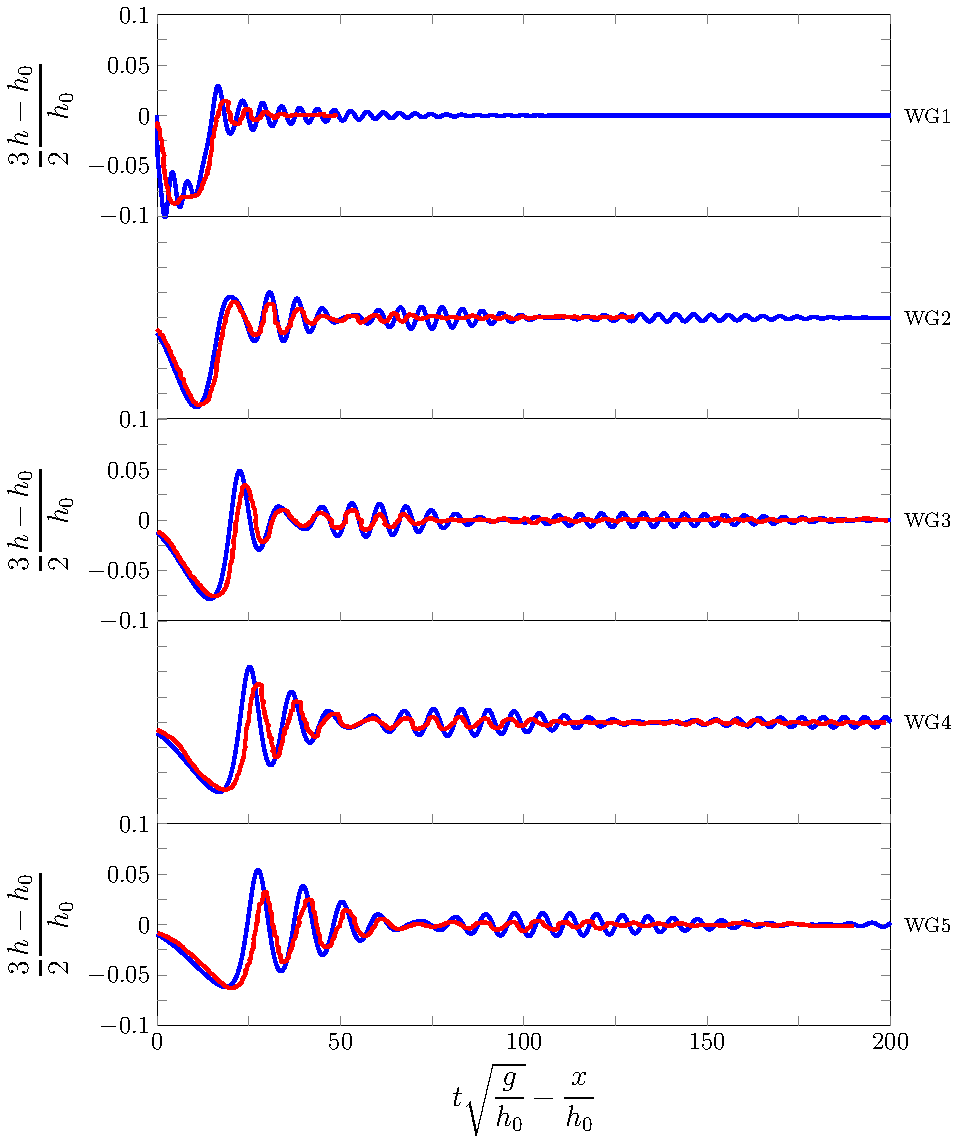
\includegraphics[width=\textwidth]{./chp6/figures/Experiment/Segur/LongWGsFEVM1cm.pdf}
	\caption{Comparison of experimental wave gauge data ({\color{red}\solidrule}) and numerical results ({\color{blue}\solidrule}) of $\text{FEVM}_2$ for the $0.01m$ rectangular depression.}
	\label{fig:Segur1cmFEVM}
\end{figure}
\begin{figure}
	\centering
	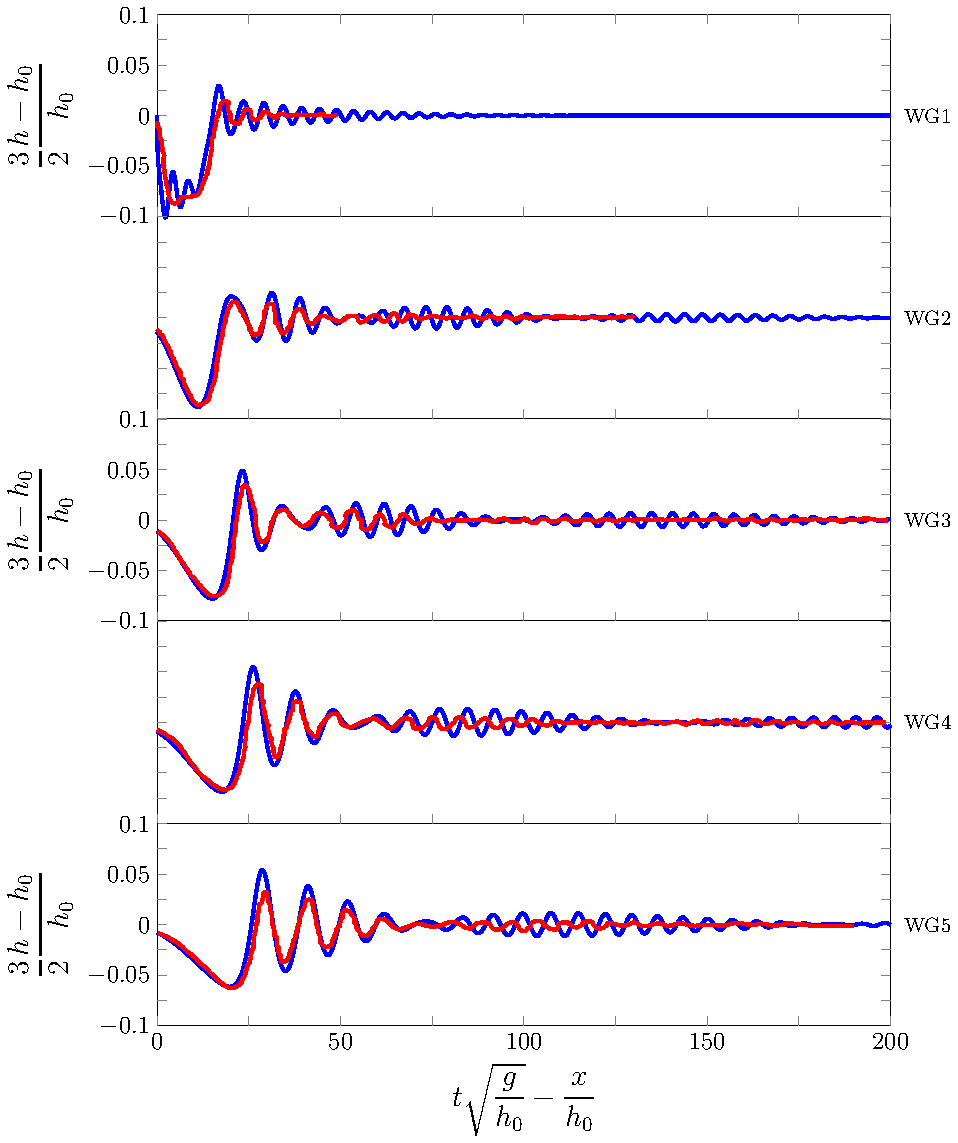
\includegraphics[width=\textwidth]{./chp6/figures/Experiment/Segur/LongWGsFDVM1cm.pdf}
	\caption{FDVM}
	\caption{Comparison of experimental wave gauge data ({\color{red}\solidrule}) and numerical results ({\color{blue}\solidrule}) of $\text{FDVM}_2$ for the $0.01m$ rectangular depression.}
	\label{fig:Segur1cmFDVM}
\end{figure} 

The numerical solutions agree well with the experimental results; particularly for the front of the dispersive wave train. While all the conserved quantities have indeed been conserved very well by the methods.  

The numerical solutions produce larger and consequently faster waves and observe oscillations in the depression which are not observed in the experimental data of wave gauge $1$. Moreover, as expected the methods produce many more oscillations than were observed experimentally. These discrepancies can be attributed to the lack of viscosity and bed friction in the Serre equations \eqref{eqn:FullSerreCon}. Furthermore, it is highly likely the experiment produced some smooth approximation to a discontinuous jump in the water depth with the down-stroke of the piston. Such a smoothing of the initial conditions will significantly attenuate the higher frequency waves in the generated dispersive wave train \cite{Pitt-2018-61}. Given these challenges the numerical methods do a very good job of replicating the experimental behaviour. 

Both $\text{FEVM}_2$ and $\text{FDVM}_2$ have produced visually identical results at this scale and have demonstrated very good conservation of all the quantities see, Tables \ref{tab:ConservationSegurFEVM1cm} and \ref{tab:ConservationSegurFDVM1cm}. Given the extensive review of these methods \cite{Pitt-2018-61} for steep gradient problems, this indicates that these solutions are indicative of true solutions of the Serre equations which are capable of reproducing experimental results.
%
\begin{table}
	\centering
	\begin{tabular}{l  c  c c}
		Quantity& $\mathcal{C}^*\left(\vecn{q}^0\right)$ & $\mathcal{C}^*\left(\vecn{q}^*\right)$ & $\mathcal{C}^*_1\left(\vecn{q}^0,\vecn{q}^*\right)$  \B\\
		\hline
		$h$ & $11.9888$ & $11.9888$ & $0$ \T\\
		$uh$ & $0$ & $7.44 \times 10^{-18}$ & $7.44 \times 10^{-18}$\\
		$G$ & $0$ & $1.56\times 10^{-18}$ & $1.56\times 10^{-18}$\\
		$\mathcal{H}$ & $5.8751$ & $5.8751$ & $5.70 \times 10^{-6}$ \B \\
		\hline
	\end{tabular}
	\caption{Initial and final total amounts and the conservation error for all conserved quantities for $\text{FEVM}_2$ numerical solution of the $0.01m$ rectangular depression.}
	\label{tab:ConservationSegurFEVM1cm}
\end{table} 
%
\begin{table}
	\centering
	\begin{tabular}{l  c  c c}
		Quantity& $\mathcal{C}^*\left(\vecn{q}^0\right)$ & $\mathcal{C}^*\left(\vecn{q}^*\right)$ & $\mathcal{C}^*_1\left(\vecn{q}^0,\vecn{q}^*\right)$ \B \\
		\hline
		$h$ & $11.9888$ & $11.9888$ & $0$ \T\\
		$uh$ & $0$ & $-1.19 \times 10^{-17}$ & $-1.19 \times 10^{-17}$\\
		$G$ & $0$ & $-8.05\times 10^{-18}$ & $-8.05\times 10^{-18}$\\
		$\mathcal{H}$ & $5.8751$ & $5.8751$ & $6.27 \times 10^{-6}$ \B\\
		\hline
	\end{tabular}
	\caption{Initial and final total amounts and the conservation error for all conserved quantities for $\text{FDVM}_2$ numerical solution of the $0.01m$ rectangular depression.}
	\label{tab:ConservationSegurFDVM1cm}
\end{table}  
 

\subsection{Results for $0.03m$ Rectangular Depression}
The wave gauge data for the numerical and experimental results for the evolution of the $0.03m$ rectangular depression are displayed in Figures \ref{fig:Segur3cmFEVM} and \ref{fig:Segur3cmFDVM} for $\text{FEVM}_2$ and $\text{FDVM}_2$ respectively. These results are reported using the same dimensionless scales as the original paper \cite{Hammack-Segur-1978-337}. The conservation of all the conserved quantities are given in Tables \ref{tab:ConservationSegurFEVM3cm} and \ref{tab:ConservationSegurFEVM3cm} for $\text{FEVM}_2$ and $\text{FDVM}_2$ respectively.
\begin{figure}
	\centering
	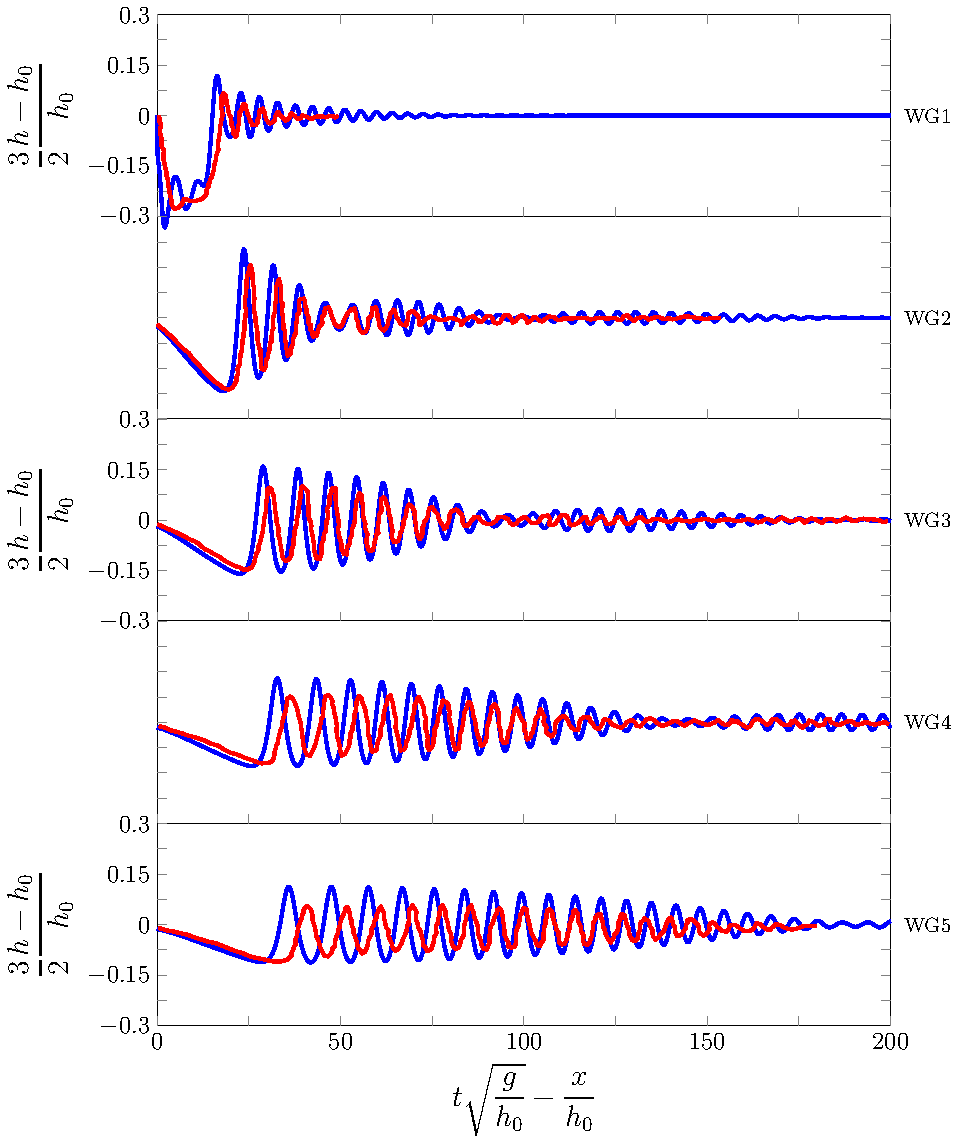
\includegraphics[width=\textwidth]{./chp6/figures/Experiment/Segur/LongWGsFEVM3cm.pdf}
	\caption{Comparison of experimental wave gauge data ({\color{red}\solidrule}) and numerical results ({\color{blue}\solidrule}) of $\text{FEVM}_2$ for the $0.03m$ rectangular depression.}
	\label{fig:Segur3cmFEVM}
\end{figure}
\begin{figure}
	\centering
	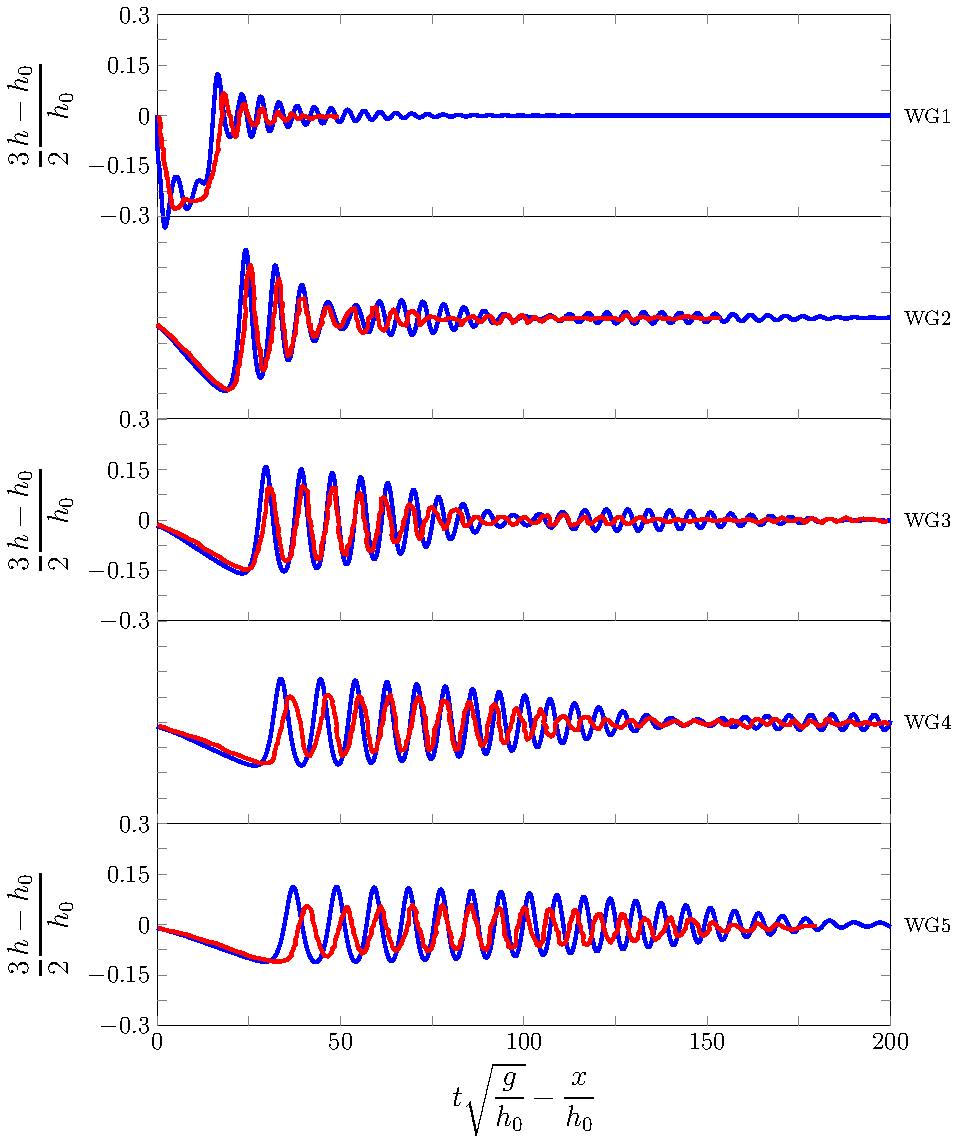
\includegraphics[width=\textwidth]{./chp6/figures/Experiment/Segur/LongWGsFDVM3cm.pdf}
	\caption{Comparison of experimental wave gauge data ({\color{red}\solidrule}) and numerical results ({\color{blue}\solidrule}) of $\text{FDVM}_2$ for the $0.03m$ rectangular depression.}
	\label{fig:Segur3cmFDVM}
\end{figure} 

Both methods again reproduce the overall behaviour of this experiment very well. Because the rectangular wave is deeper, this experiment provides a more rigorous test for the numerical methods. However, increasing the depth also strengthens the causes of the discrepancy between the experimental results and the numerical solutions of the Serre equations. This can be seen most acutely for the amplitude and speed of the generated waves.

Since the rectangular depression is larger the numerical methods have a larger error in conservation for all the quantities as compared to the $0.01m$ rectangular depression except mass; which is conserved exactly. For $G$ and momentum these errors are around machine epsilon and can be disregarded, so that only the conservation of energy is significantly effected. Even with this larger error, all quantities are still well conserved by the numerical methods, suggesting that the numerical solutions well approximate the true solutions of the Serre equations. 

These experiments have been well replicated by the numerical methods, and given the resolution and error in conservation and the extensive study summarised in Chapter \ref{chp:Serreeqns}; these results demonstrate the accuracy of the numerical methods in the presence of steep gradients in the free surface.       
%
\begin{table}
	\centering
	\begin{tabular}{l  c  c c}
		Quantity& $\mathcal{C}^*\left(\vecn{q}^0\right)$ & $\mathcal{C}^*\left(\vecn{q}^*\right)$ & $\mathcal{C}^*_1\left(\vecn{q}^0,\vecn{q}^*\right)$ \B \\
		\hline 
		$h$ & $11.9644$ & $11.9644$ & $0$ \T\\
		$uh$ & $0$ & $-7.75 \times 10^{-17}$ & $-7.75\times 10^{-17}$\\
		$G$ & $0$ & $-3.33\times 10^{-16}$ & $-3.33\times 10^{-16}$\\
		$\mathcal{H}$ & $5.8560$ & $5.8552$ & $1.24 \times 10^{-4}$  \B \\
		\hline
	\end{tabular}
	\caption{Initial and final total amounts and the conservation error for all conserved quantities for $\text{FEVM}_2$ numerical solution of the $0.03m$ rectangular depression.}
	\label{tab:ConservationSegurFEVM3cm}
\end{table} 
%
\begin{table}
	\centering
	\begin{tabular}{l  c  c c}
		Quantity& $\mathcal{C}^*\left(\vecn{q}^0\right)$ & $\mathcal{C}^*\left(\vecn{q}^*\right)$ & $\mathcal{C}^*_1\left(\vecn{q}^0,\vecn{q}^*\right)$ \B \\
		\hline
		$h$ & $11.9644$ & $11.9644$ & $0$ \T\\
		$uh$ & $0$ & $-9.09 \times 10^{-17}$ & $-9.09 \times 10^{-17}$\\
		$G$ & $0$ & $-1.16\times 10^{-16}$ & $-1.16\times 10^{-16}$\\
		$\mathcal{H}$ & $5.8560$ & $5.8552$ & $1.30 \times 10^{-4}$ \B\\
		\hline
	\end{tabular}
	\caption{Initial and final total amounts and the conservation error for all conserved quantities for $\text{FDVM}_2$ numerical solution of the $0.03m$ rectangular depression.}
	\label{tab:ConservationSegurFDVM3cm}
\end{table}  

\section{Periodic Waves Over A Submerged Bar}
\label{sec:PeriodicWavessubBar}
Beji and Battjes conducted a series of experiments investigating the effect of submerged bars on the propagation of periodic waves \cite{Beji-Battjes-1993-151,Beji-Battjes-1994-1}. The behaviour of these experiments were mainly driven by the dispersion properties of the waves and their interaction with variations in bathymetry. Therefore, these experiments serve as a benchmark for the ability of the numerical schemes to accurately model the interaction of variable bathymetry and dispersive waves. For our purposes we will focus on the monochromatic wave experiments of \citet{Beji-Battjes-1994-1}.

The experiments of \citet{Beji-Battjes-1994-1} were conducted in a wave tank $37.7m$ long, $0.8m$ wide and $0.75m$ high. A diagram of the longitudinal section of the wave tank is given in Figure \ref{fig:BejiWT}. There are seven wave gauges at the following locations; $5.7m$, $10.5m$, $12.5m$, $13.5m$, $14.5m$, $15.7m$ and $17.3m$. Waves are generated from a piston-type wave maker located at $0m$ and travel on the initially still water $0.4m$ deep to the right, over the submerged trapezoidal bar and are absorbed by a sloping beach.
\begin{figure}
	\centering
	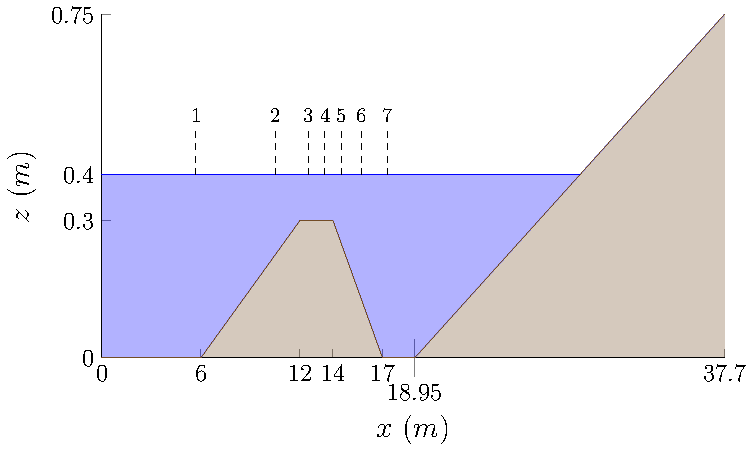
\includegraphics[width=\textwidth]{./chp6/figures/Experiment/Beji/BejiTank.pdf}
	\caption{The flume configuration with water (\squareF{blue}) and the bed (\squareF{brown!80!black}) for the Beji experiments, with the wave gauge locations marked.}
	\label{fig:BejiWT}
\end{figure}

Two sinusoidal monochromatic non-breaking wave experiments were conducted. A low frequency one with a wavelength $\lambda \approx 3.69m$ and a period of $T = 2s$, and a high frequency one with $\lambda \approx 2.05m$ and a period of $T = 1.25s$. Both experiments had a wave amplitude of $0.01m$ and so both had the same small non-linearity parameter $\epsilon = 0.01 / 0.4 = 0.025$. 

We numerically simulated these experiments over the spatial domain $\left[5.7m,150m\right]$ with $\Delta x = 0.1 / 2^4 m \approx 0.0063m$ and $\Delta t = Sp / 2^5 s \approx 0.0012s$ where $Sp = 0.039 s$ is the experimental sampling period. These $\Delta x$ and $\Delta t$ values satisfy the CFL condition, \eqref{eqn:CFLcond}. In our numerical experiments only the submerged trapezoidal bar is present, and the sloping beach is replaced with a very long horizontal bed that ensures that we do not observe any effects from the Dirichlet boundary conditions at the downstream boundary.  

To simulate the incoming waves at the upstream boundary we used the first wave gauge as our left boundary condition together with linear extrapolation to calculate the other required $h$ values in the left ghost cell. The velocity boundary conditions were calculated from the height values in the same way as \citet{Beji-Battjes-1994-1}
\begin{equation*}
u(x,t) = \sqrt{g h_0} \; \dfrac{h(x,t) - h_0}{h(x,t)}.
\end{equation*}
Finally the boundary conditions for $G$ were calculated using the boundary conditions for $h$ and $u$. 

We shall now present our numerical results for the low and high frequency experiments.
%
\subsection{Low Frequency Results}
A comparison of the wave heights $\eta$ of the experimental and numerical results are located in Figures \ref{fig:BejislWG1to4FEVM} and \ref{fig:BejislWG5to7FEVM} for $\text{FEVM}_2$ and Figures \ref{fig:BejislWG1to4FDVM} and \ref{fig:BejislWG5to7FDVM} for $\text{FDVM}_2$. These numerical schemes both produce identical results for all wave gauges and so this benchmark does not help us discriminate between these two methods. 
\begin{figure}
	\centering
	\begin{subfigure}{0.5\textwidth}
		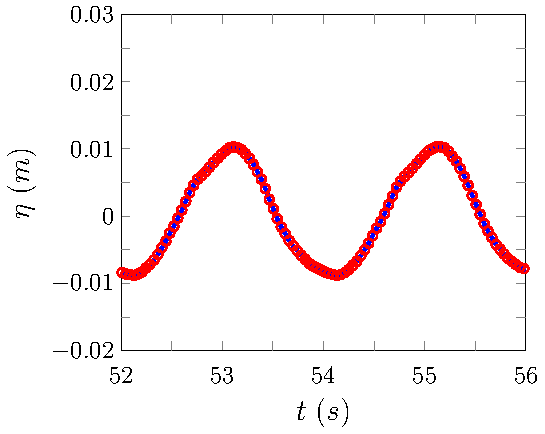
\includegraphics[width=\textwidth]{./chp6/figures/Experiment/Beji/sl/FEVMWG1.pdf}
		\subcaption{Wave Gauge $1$}
		\vspace{0.5cm}
	\end{subfigure}%
	\begin{subfigure}{0.5\textwidth}
		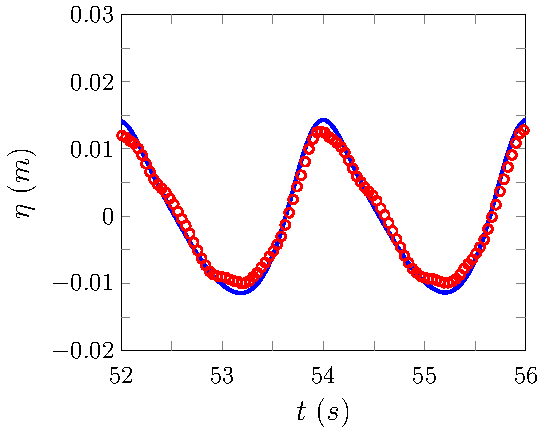
\includegraphics[width=\textwidth]{./chp6/figures/Experiment/Beji/sl/FEVMWG2.pdf}
		\subcaption{Wave Gauge $2$}
		\vspace{0.5cm}
	\end{subfigure}
	\begin{subfigure}{0.5\textwidth}
		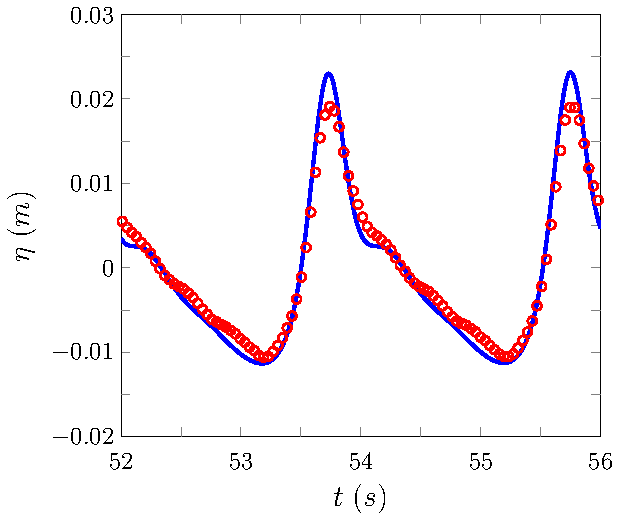
\includegraphics[width=\textwidth]{./chp6/figures/Experiment/Beji/sl/FEVMWG3.pdf}
		\subcaption{Wave Gauge $3$}
		\vspace{0.5cm}
	\end{subfigure}%
	\begin{subfigure}{0.5\textwidth}
		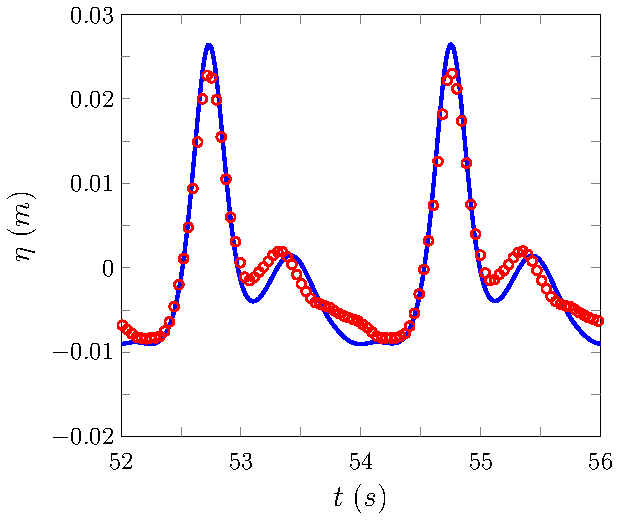
\includegraphics[width=\textwidth]{./chp6/figures/Experiment/Beji/sl/FEVMWG4.pdf}
		\subcaption{Wave Gauge $4$}
		\vspace{0.5cm}
	\end{subfigure}
	\caption{Comparison of the wave heights $\eta$ of the numerical results for the $\text{FEVM}_2$ ({\color{blue}\solidrule}) and the experimental results (\circlet{red}) for wave gauges $1$ - $4$ for the low frequency experiment.}
	\label{fig:BejislWG1to4FEVM}
\end{figure}
%
\begin{figure}
	\centering
	\begin{subfigure}{0.5\textwidth}
		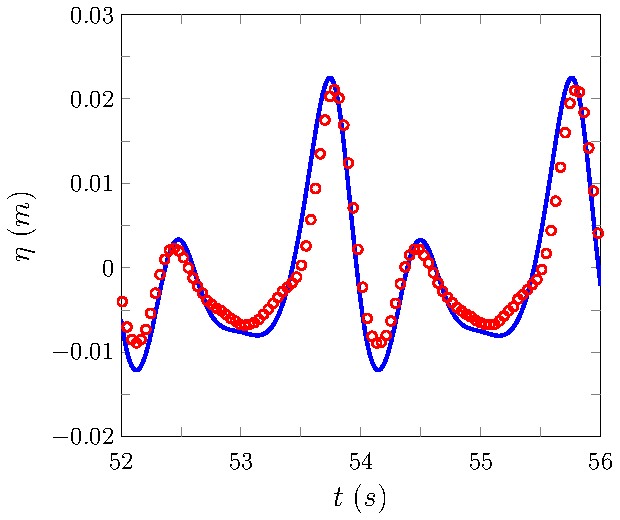
\includegraphics[width=\textwidth]{./chp6/figures/Experiment/Beji/sl/FEVMWG5.pdf}
		\subcaption{Wave Gauge $5$}
		\vspace{0.5cm}
	\end{subfigure}%
	\begin{subfigure}{0.5\textwidth}
		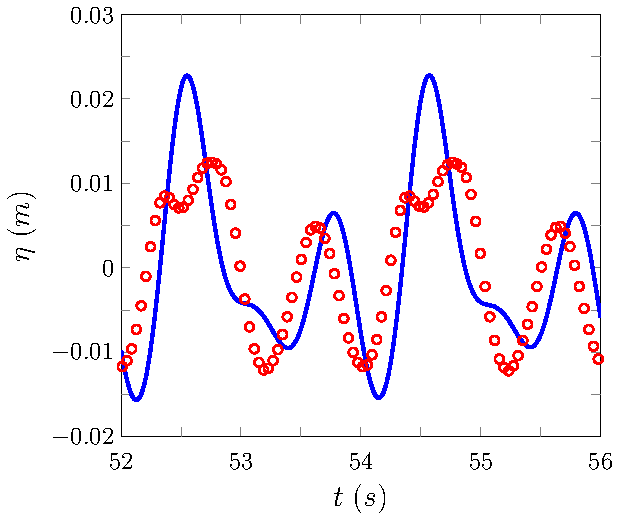
\includegraphics[width=\textwidth]{./chp6/figures/Experiment/Beji/sl/FEVMWG6.pdf}
		\subcaption{Wave Gauge $6$}
		\vspace{0.5cm}
	\end{subfigure}
	\begin{subfigure}{0.5\textwidth}
		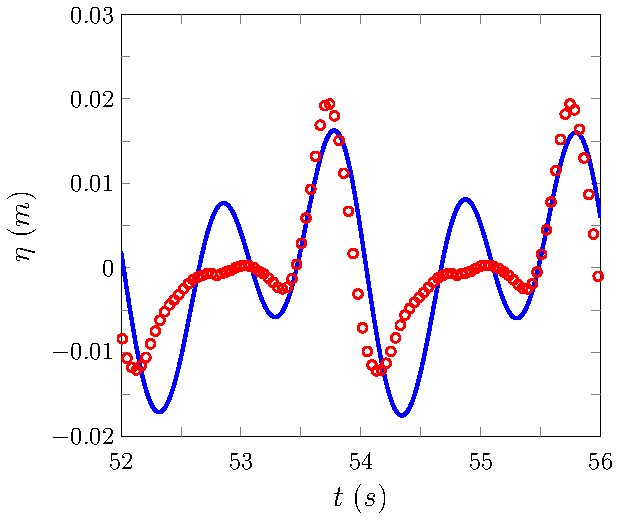
\includegraphics[width=\textwidth]{./chp6/figures/Experiment/Beji/sl/FEVMWG7.pdf}
		\subcaption{Wave Gauge $7$}
		\vspace{0.5cm}
	\end{subfigure}
	\caption{Comparison of the wave heights $\eta$ of the numerical results for the $\text{FEVM}_2$ ({\color{blue}\solidrule}) and the experimental results (\circlet{red}) for wave gauges $5$ - $7$ for the low frequency experiment.}
	\label{fig:BejislWG5to7FEVM}
\end{figure}
%
\begin{figure}
	\centering
	\begin{subfigure}{0.5\textwidth}
		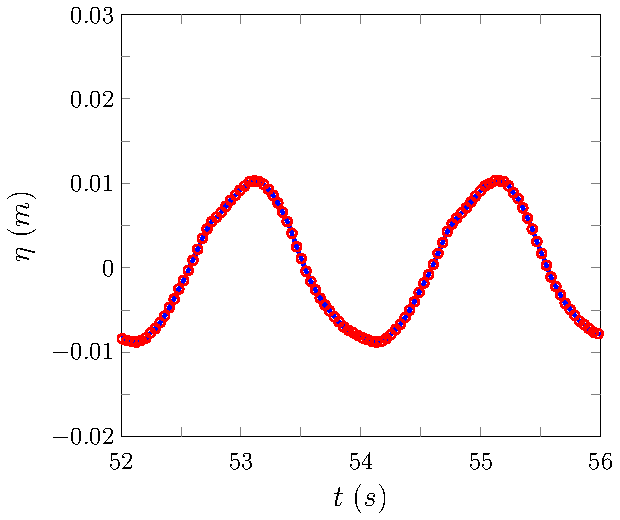
\includegraphics[width=\textwidth]{./chp6/figures/Experiment/Beji/sl/FDVMWG1.pdf}
		\subcaption{Wave Gauge $1$}
		\vspace{0.5cm}
	\end{subfigure}%
	\begin{subfigure}{0.5\textwidth}
		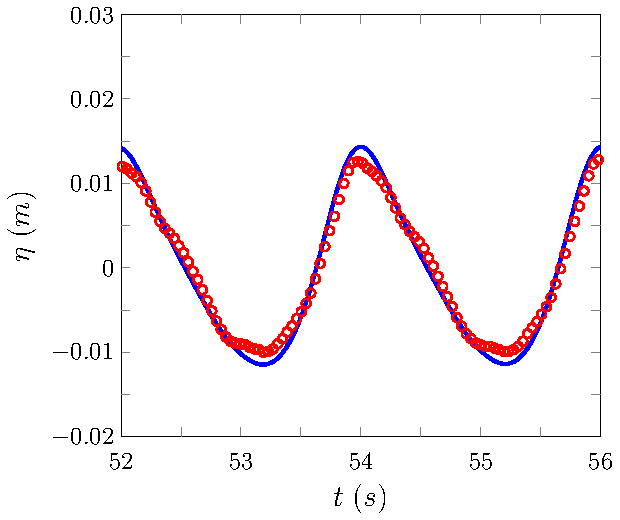
\includegraphics[width=\textwidth]{./chp6/figures/Experiment/Beji/sl/FDVMWG2.pdf}
		\subcaption{Wave Gauge $2$}
		\vspace{0.5cm}
	\end{subfigure}
	\begin{subfigure}{0.5\textwidth}
		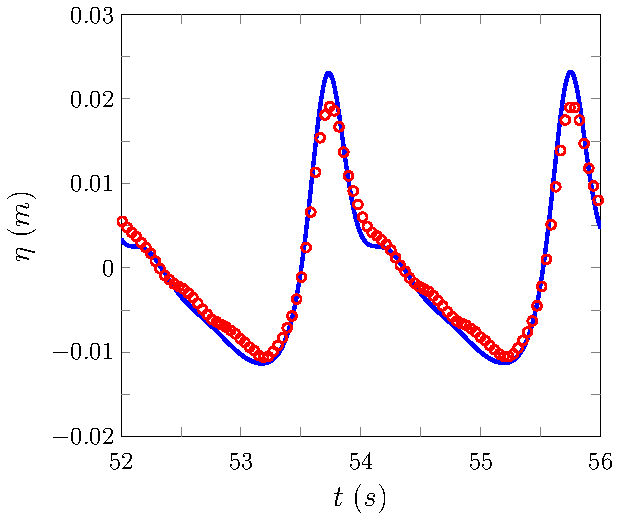
\includegraphics[width=\textwidth]{./chp6/figures/Experiment/Beji/sl/FDVMWG3.pdf}
		\subcaption{Wave Gauge $3$}
		\vspace{0.5cm}
	\end{subfigure}%
	\begin{subfigure}{0.5\textwidth}
		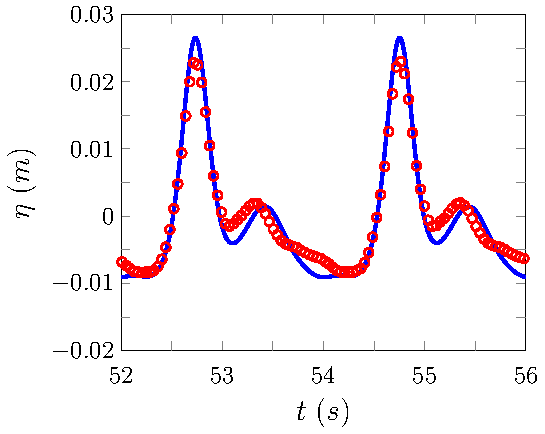
\includegraphics[width=\textwidth]{./chp6/figures/Experiment/Beji/sl/FDVMWG4.pdf}
		\subcaption{Wave Gauge $4$}
		\vspace{0.5cm}
	\end{subfigure}
	\caption{Comparison of the wave heights $\eta$ of the numerical results for the $\text{FDVM}_2$ ({\color{blue}\solidrule}) and the experimental results (\circlet{red}) for wave gauges $1$ - $4$ for the low frequency experiment.}
	\label{fig:BejislWG1to4FDVM}
\end{figure}
%
\begin{figure}
	\centering
	\begin{subfigure}{0.5\textwidth}
		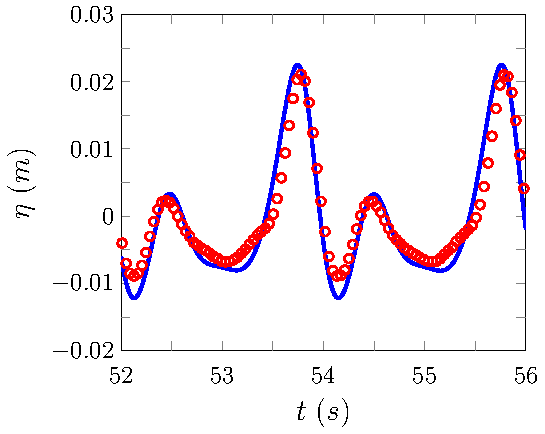
\includegraphics[width=\textwidth]{./chp6/figures/Experiment/Beji/sl/FDVMWG5.pdf}
		\subcaption{Wave Gauge $5$}
		\vspace{0.5cm}
	\end{subfigure}%
	\begin{subfigure}{0.5\textwidth}
		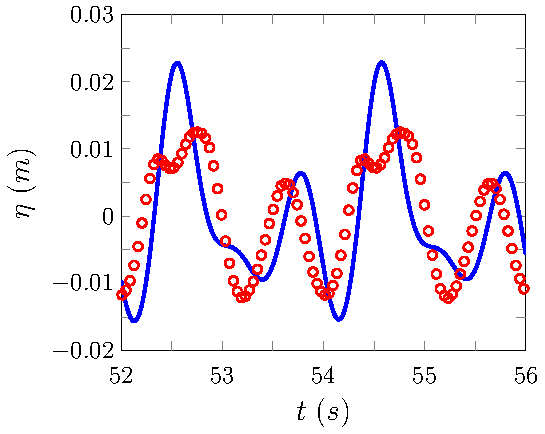
\includegraphics[width=\textwidth]{./chp6/figures/Experiment/Beji/sl/FDVMWG6.pdf}
		\subcaption{Wave Gauge $6$}
		\vspace{0.5cm}
	\end{subfigure}
	\begin{subfigure}{0.5\textwidth}
		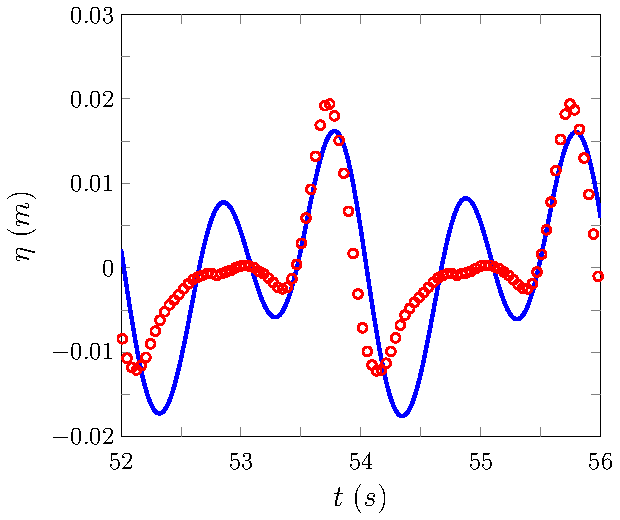
\includegraphics[width=\textwidth]{./chp6/figures/Experiment/Beji/sl/FDVMWG7.pdf}
		\subcaption{Wave Gauge $7$}
		\vspace{0.5cm}
	\end{subfigure}
	\caption{Comparison of the wave heights $\eta$ of the numerical results for the $\text{FDVM}_2$ ({\color{blue}\solidrule}) and the experimental results (\circlet{red}) for wave gauges $5$ - $7$ for the low frequency experiment.}
	\label{fig:BejislWG5to7FDVM}
\end{figure}

These results demonstrate the ability of these numerical methods to recreate the experimental results, particularly for wave gauge $1$ to $5$ where the agreement between experimental and numerical results is best. Results at these gauges validate the numerical schemes for simulating shoaling of dispersive waves as these wave gauges are all located on the windward side of the submerged bar where shoaling occurs in the experiment. 

The numerical results for wave gauges $6$ and $7$ on the leeward side capture some of the wave behaviour but their agreement with the experiments results is much worse. The inadequacy of the numerical results here appears to be due to the discrepancy between the dispersion properties of the Serre equations and actual water waves \cite{Beji-Battjes-1994-1,Lannes-2013}.

The dispersion terms in the Serre equations are vital to recreating the experimental results for wave gauges $2$ to $5$, as non-dispersive equations such as the SWWE are not capable of accurately simulating this experiment \cite{Pitt-2017-1725}.

\subsection{High Frequency Results}
The wave heights of the experimental and numerical results are given in Figures \ref{fig:BejishWG1to4FEVM} and \ref{fig:BejishWG5to7FEVM} for $\text{FEVM}_2$. While the results for $\text{FDVM}_2$ are given in Figures \ref{fig:BejishWG1to4FDVM} and \ref{fig:BejishWG5to7FDVM}. As for the low frequency experiment $\text{FEVM}_2$ and $\text{FDVM}_2$ produce identical results for all wave gauges at this scale and so this benchmark does not discriminate between these two methods. 
%
\begin{figure}
	\centering
	\begin{subfigure}{0.5\textwidth}
		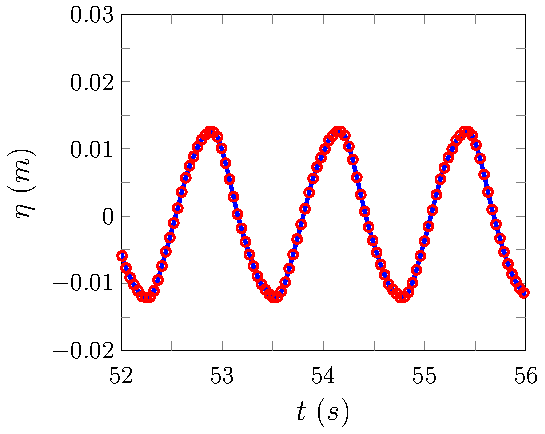
\includegraphics[width=\textwidth]{./chp6/figures/Experiment/Beji/sh/FEVMWG1.pdf}
		\subcaption{Wave Gauge $1$}
		\vspace{0.5cm}
	\end{subfigure}%
	\begin{subfigure}{0.5\textwidth}
		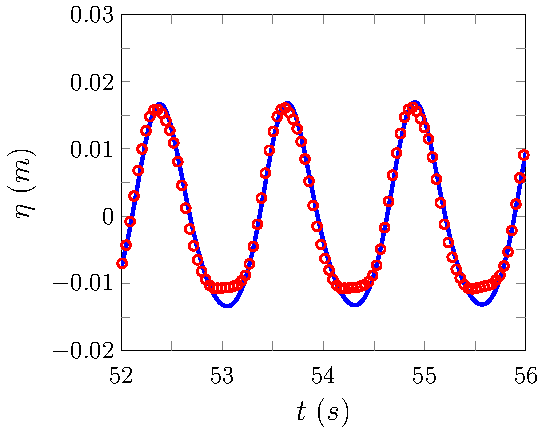
\includegraphics[width=\textwidth]{./chp6/figures/Experiment/Beji/sh/FEVMWG2.pdf}
		\subcaption{Wave Gauge $2$}
		\vspace{0.5cm}
	\end{subfigure}
	\begin{subfigure}{0.5\textwidth}
		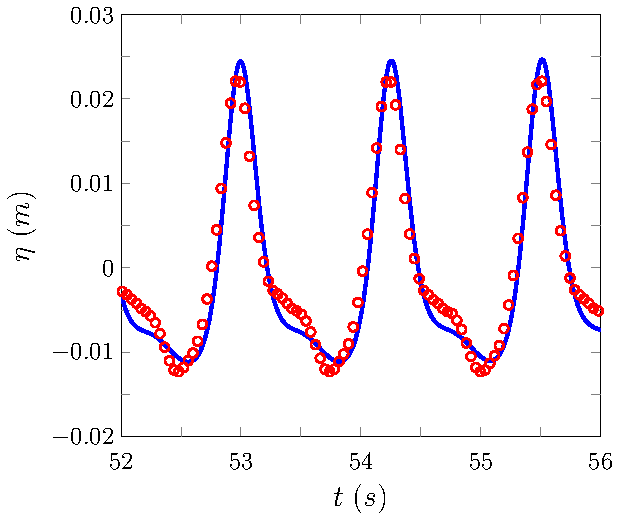
\includegraphics[width=\textwidth]{./chp6/figures/Experiment/Beji/sh/FEVMWG3.pdf}
		\subcaption{Wave Gauge $3$}
		\vspace{0.5cm}
	\end{subfigure}%
	\begin{subfigure}{0.5\textwidth}
		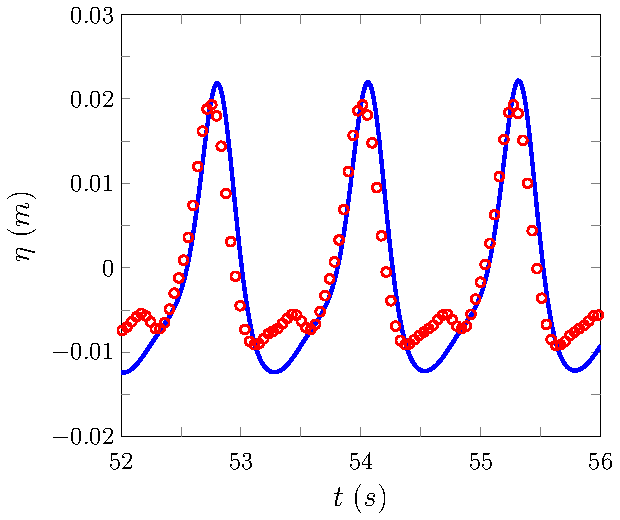
\includegraphics[width=\textwidth]{./chp6/figures/Experiment/Beji/sh/FEVMWG4.pdf}
		\subcaption{Wave Gauge $4$}
		\vspace{0.5cm}
	\end{subfigure}
	\caption{Comparison of the wave heights $\eta$ of the numerical results for the $\text{FEVM}_2$ ({\color{blue}\solidrule}) and the experimental results (\circlet{red}) for wave gauges $1$ - $4$ for the low frequency experiment.}
	\label{fig:BejishWG1to4FEVM}
\end{figure}
%
\begin{figure}
	\centering
	\begin{subfigure}{0.5\textwidth}
		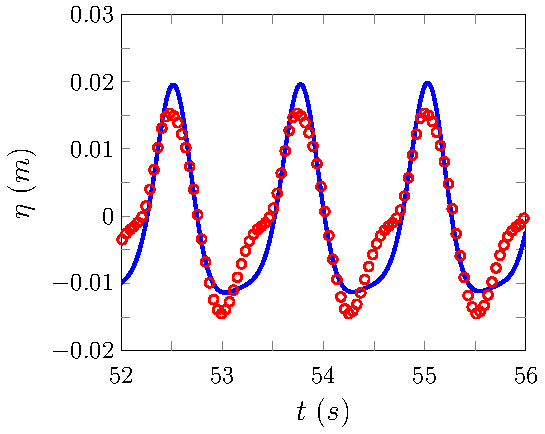
\includegraphics[width=\textwidth]{./chp6/figures/Experiment/Beji/sh/FEVMWG5.pdf}
		\subcaption{Wave Gauge $5$}
		\vspace{0.5cm}
	\end{subfigure}%
	\begin{subfigure}{0.5\textwidth}
		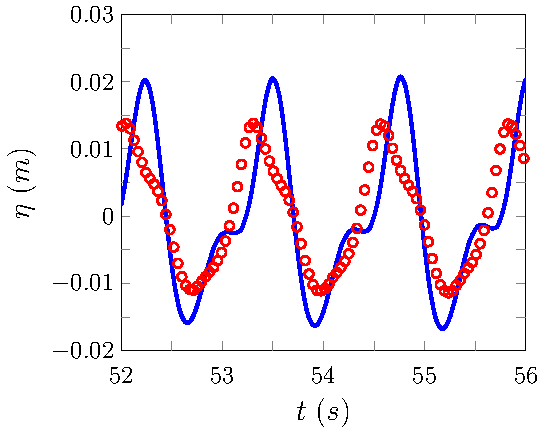
\includegraphics[width=\textwidth]{./chp6/figures/Experiment/Beji/sh/FEVMWG6.pdf}
		\subcaption{Wave Gauge $6$}
		\vspace{0.5cm}
	\end{subfigure}
	\begin{subfigure}{0.5\textwidth}
		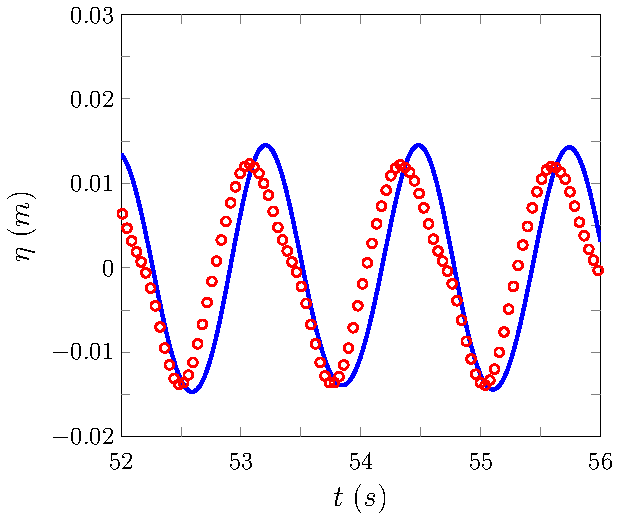
\includegraphics[width=\textwidth]{./chp6/figures/Experiment/Beji/sh/FEVMWG7.pdf}
		\subcaption{Wave Gauge $7$}
		\vspace{0.5cm}
	\end{subfigure}
	\caption{Comparison of the wave heights $\eta$ of the numerical results for the $\text{FEVM}_2$ ({\color{blue}\solidrule}) and the experimental results (\circlet{red}) for wave gauges $5$ - $7$ for the high frequency experiment.}
	\label{fig:BejishWG5to7FEVM}
\end{figure}
%
\begin{figure}
	\centering
	\begin{subfigure}{0.5\textwidth}
		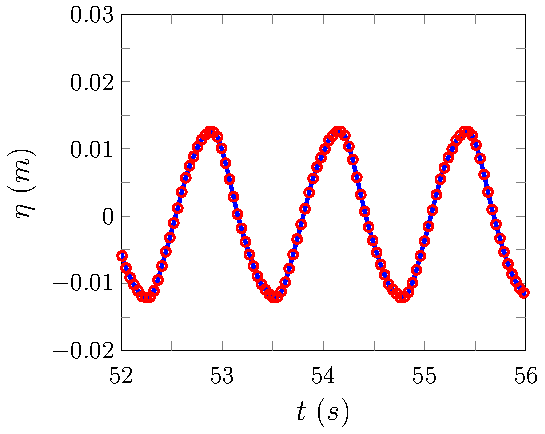
\includegraphics[width=\textwidth]{./chp6/figures/Experiment/Beji/sh/FDVMWG1.pdf}
		\subcaption{Wave Gauge $1$}
		\vspace{0.5cm}
	\end{subfigure}%
	\begin{subfigure}{0.5\textwidth}
		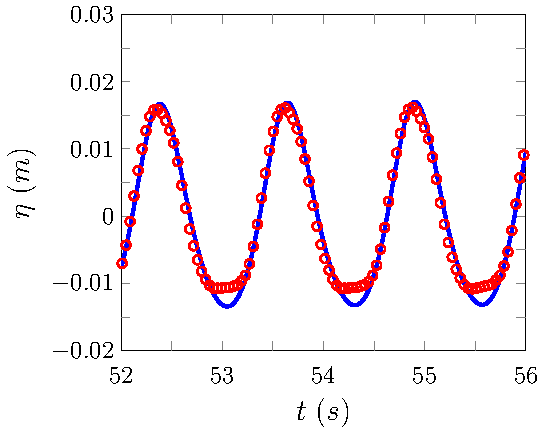
\includegraphics[width=\textwidth]{./chp6/figures/Experiment/Beji/sh/FDVMWG2.pdf}
		\subcaption{Wave Gauge $2$}
		\vspace{0.5cm}
	\end{subfigure}
	\begin{subfigure}{0.5\textwidth}
		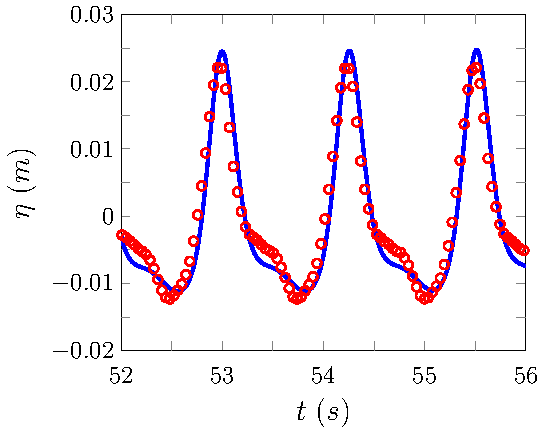
\includegraphics[width=\textwidth]{./chp6/figures/Experiment/Beji/sh/FDVMWG3.pdf}
		\subcaption{Wave Gauge $3$}
		\vspace{0.5cm}
	\end{subfigure}%
	\begin{subfigure}{0.5\textwidth}
		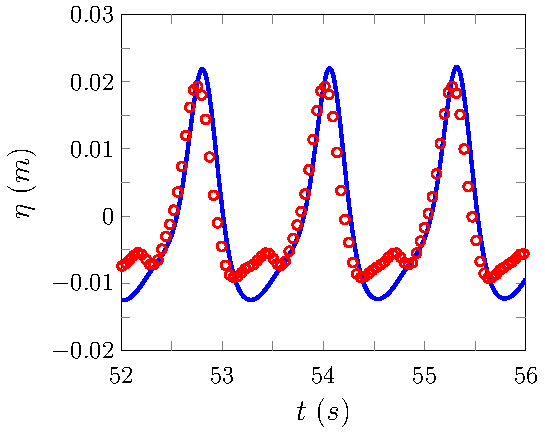
\includegraphics[width=\textwidth]{./chp6/figures/Experiment/Beji/sh/FDVMWG4.pdf}
		\subcaption{Wave Gauge $4$}
		\vspace{0.5cm}
	\end{subfigure}
	\caption{Comparison of the wave heights $\eta$ of the numerical results for the $\text{FDVM}_2$ ({\color{blue}\solidrule}) and the experimental results (\circlet{red}) for wave gauges $1$ - $4$ for the high frequency experiment.}
	\label{fig:BejishWG1to4FDVM}
\end{figure}
%
\begin{figure}
	\centering
	\begin{subfigure}{0.5\textwidth}
		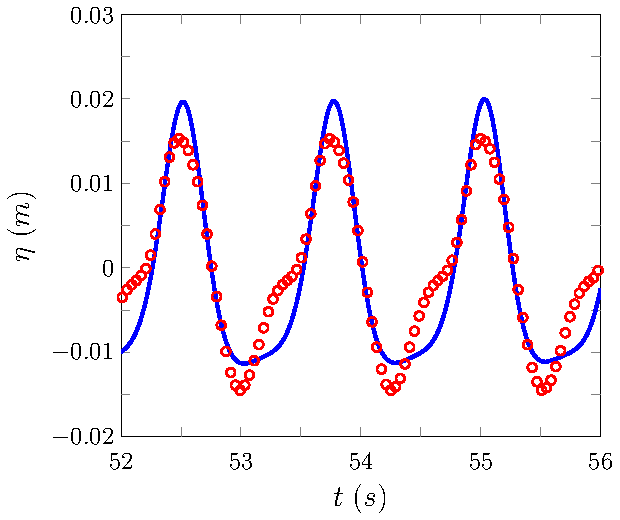
\includegraphics[width=\textwidth]{./chp6/figures/Experiment/Beji/sh/FDVMWG5.pdf}
		\subcaption{Wave Gauge $5$}
		\vspace{0.5cm}
	\end{subfigure}%
	\begin{subfigure}{0.5\textwidth}
		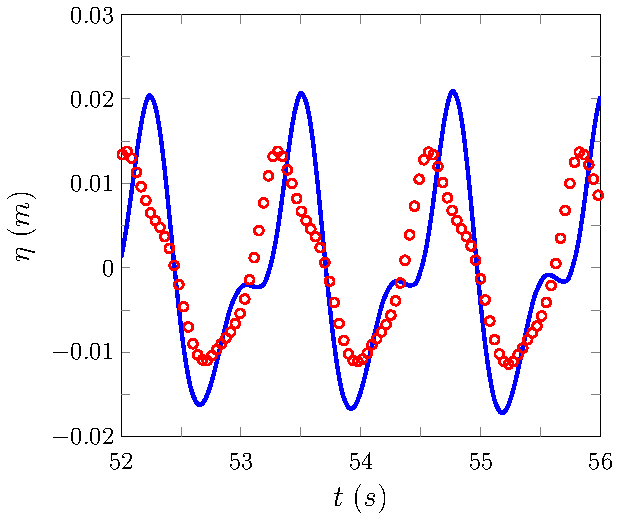
\includegraphics[width=\textwidth]{./chp6/figures/Experiment/Beji/sh/FDVMWG6.pdf}
		\subcaption{Wave Gauge $6$}
		\vspace{0.5cm}
	\end{subfigure}
	\begin{subfigure}{0.5\textwidth}
		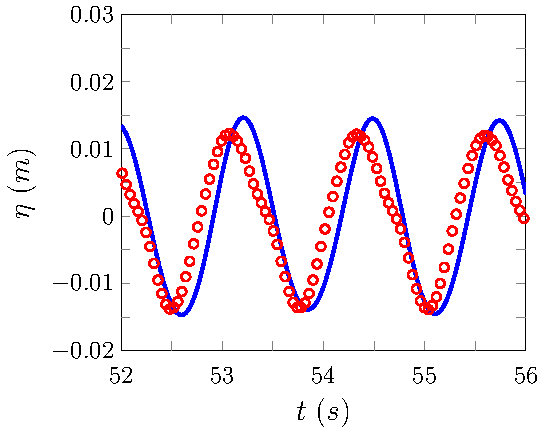
\includegraphics[width=\textwidth]{./chp6/figures/Experiment/Beji/sh/FDVMWG7.pdf}
		\subcaption{Wave Gauge $7$}
		\vspace{0.5cm}
	\end{subfigure}
	\caption{Comparison of the wave heights $\eta$ of the numerical results for the $\text{FDVM}_2$ ({\color{blue}\solidrule}) and the experimental results (\circlet{red}) for wave gauges $5$ - $7$ for the high frequency experiment.}
	\label{fig:BejishWG5to7FDVM}
\end{figure}

As in the low frequency experiment we observe that the numerical results perform well on the windward side of the slope for wave gauges $1$ to $4$ but perform poorly for the leeward side of the slope for wave gauges $5$ to $7$. With the high frequency experiment we see the divergence between the numerical and experimental results earlier than the low frequency experiment, so that now wave gauge 5 which is on the leeward side exhibits a significant difference between the numerical and experimental results. As in the low frequency example this is caused by the difference in the dispersion relations of the Serre equations and the linear theory for water waves \cite{Beji-Battjes-1994-1,Lannes-2013}. Because the difference between the dispersion relation of the Serre equations and water waves is largest for higher frequency and therefore for shorter waves \cite{Barthelemy-2004-315} the earlier divergence between experimental and numerical results is not surprising. 

These numerical results for the $\text{FDVM}_2$ and $\text{FEVM}_2$ agree well with other numerical results for weakly dispersive equations without improved dispersion properties for the simulation of periodic waves over a submerged bar in the literature \cite{Beji-Battjes-1994-1,Lannes-2013,Li-2014-169,Zhang-2013-13}. Therefore, without changing the underlying partial differential equations, our numerical methods perform as well as other numerical schemes in the literature at recreating the experimental results of \citet{Beji-Battjes-1994-1}.

\section{Solitary Wave Over a Fringing Reef}
%Chris wants more nonlinear, shallow water paramtrers there
To study the evolution of waves on fringing reefs a series of experiments were conducted by \citet{Roeber-2010}. These experiments were performed in a wave tank $3.66m$ wide, $83.7m$ long and $4.57m$ high with a removable bed that allowed for the wide range of experiments reported by \citet{Roeber-2010}. We have computationally modelled the experiment with the bathymetry displayed in Figure \ref{fig:RoeberWT}, where a solitary wave is generated from the wave maker at $0m$ and is recorded at the wave gauges $17.6m$, $28.6m$, $35.9m$, $40.6m$, $44.3m$, $46.1m$, $48.2m$, $50.4m$, $54.4m$, $58.0m$, $61.7m$, $65.4m$, $72.7m$ and $80.0m$ downstream of the wave maker.
\begin{figure}
	\centering
	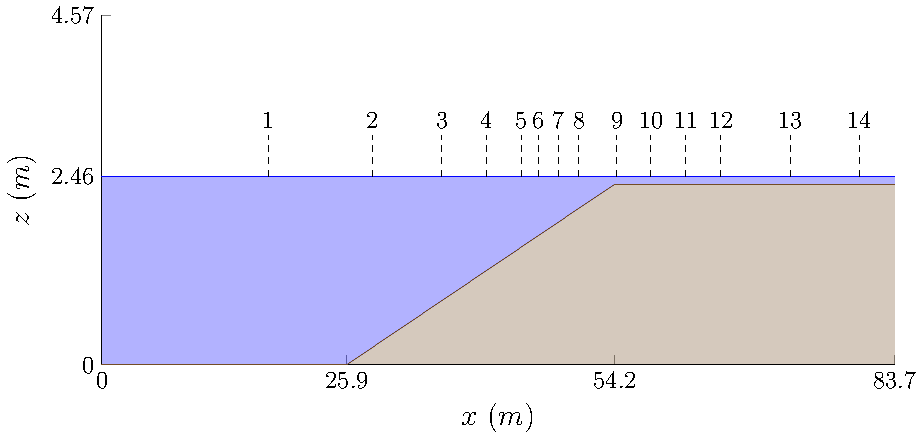
\includegraphics[width=\textwidth]{./chp6/figures/Experiment/Roeber/Trial8/WaveTank.pdf}
	\caption{Diagram demonstrating the water (\squareF{blue}) and the ground  (\squareF{brown!80!black}) for the solitary wave over a fringing reef experiment, with the wave gauge locations marked.}
	\label{fig:RoeberWT}
\end{figure}

This experiment investigates the behaviour of waves with high nonlinearity $ \epsilon \approx 1.23/2.46 = 0.5$ as it shoals over a linear bed into a very shallow body of water. Given the high nonlinearity of this wave, it is not surprising that as it shoals it becomes a plunging breaker by $t \approx 32s$ with an elliptical air cavity observed at $t \approx 33s$ \cite{Roeber-2010}. As with other depth averaged equations, the Serre equations cannot naively model breaking waves so this experiment is not an entirely appropriate test of the numerical methods, particularly after $t=32s$.

This experiment was numerically modelled on the domain $[17.6m , 400m]$ and was run until $t = 60s$ after which the reflections from the downstream end of the tank become significant in the experiment. The beginning of the domain was chosen so that wave gauge $1$ could be used as the left boundary conditions, where the technique for the boundary condition in section \ref{sec:PeriodicWavessubBar} was employed. The spatial resolution was $\Delta x = 0.025m$ and the temporal resolution was $\Delta t = Sp / 8 s = 0.0025$ where $Sp = 0.02s$ was the sampling period of the wave gauges, these spatial and temporal resolutions satisfy the CFL condition \eqref{eqn:CFLcond}. The right edge of the domain used Dirichlet boundary conditions, since the domain was so large no effects from the downstream boundary were observed throughout the numerical simulation. 

\subsection{Results}
The wave gauge results comparing the numerical and experimental data are displayed in Figures \ref{fig:Roeber8WG1to5FEVM}, \ref{fig:Roeber8WG6to10FEVM} and \ref{fig:Roeber8WG11to14FEVM} for $\text{FEVM}_2$ and \ref{fig:Roeber8WG1to5FDVM} and \ref{fig:Roeber8WG6to9FDVM} for $\text{FDVM}_2$.
\begin{figure}
	\centering
	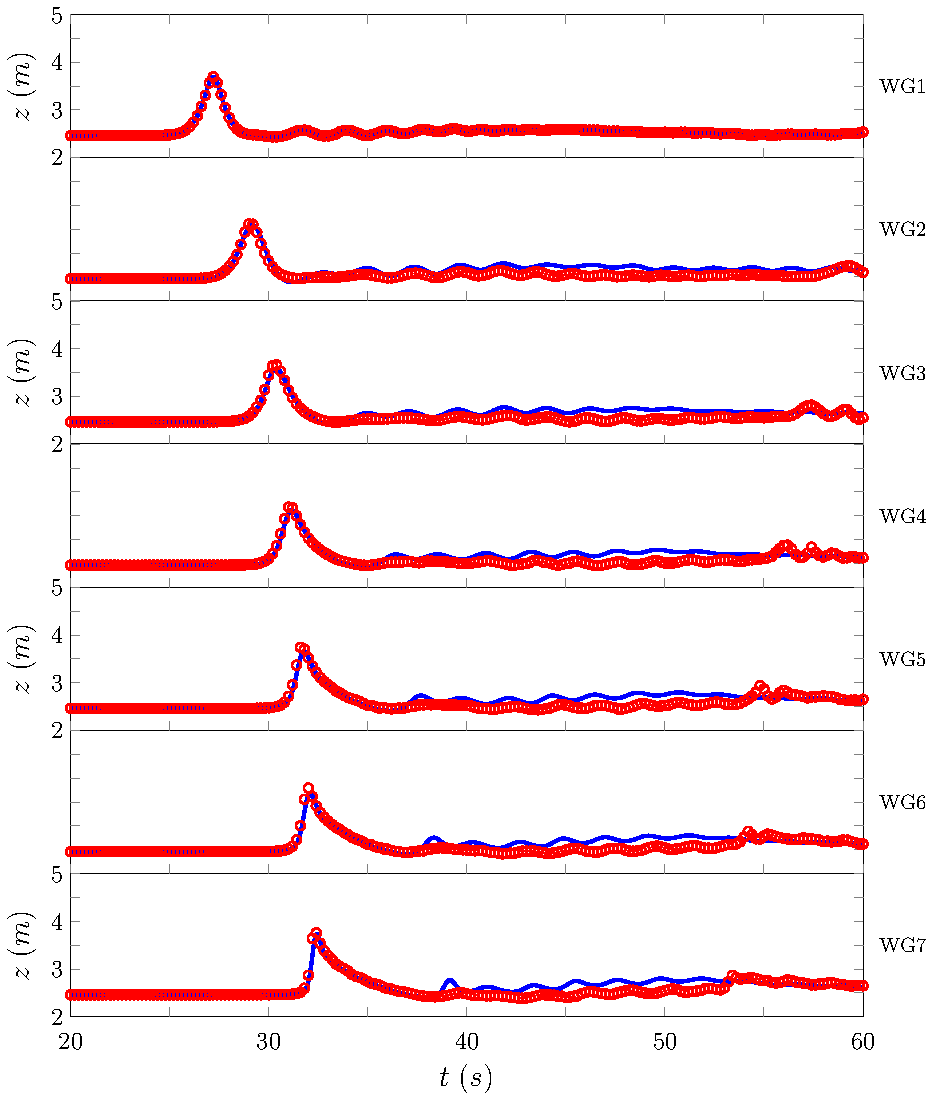
\includegraphics[width=\textwidth]{./chp6/figures/Experiment/Roeber/Trial8/FEVM/LongWGs1.pdf}
	\caption{Comparison of the experimental (\circlet{red}) and numerical ({\color{blue}\solidrule}) wave gauge data produced by $\text{FEVM}_2$ for gauges $1$ to $5$.}
	\label{fig:Roeber8WG1to5FEVM}
\end{figure}
\begin{figure}
	\centering
	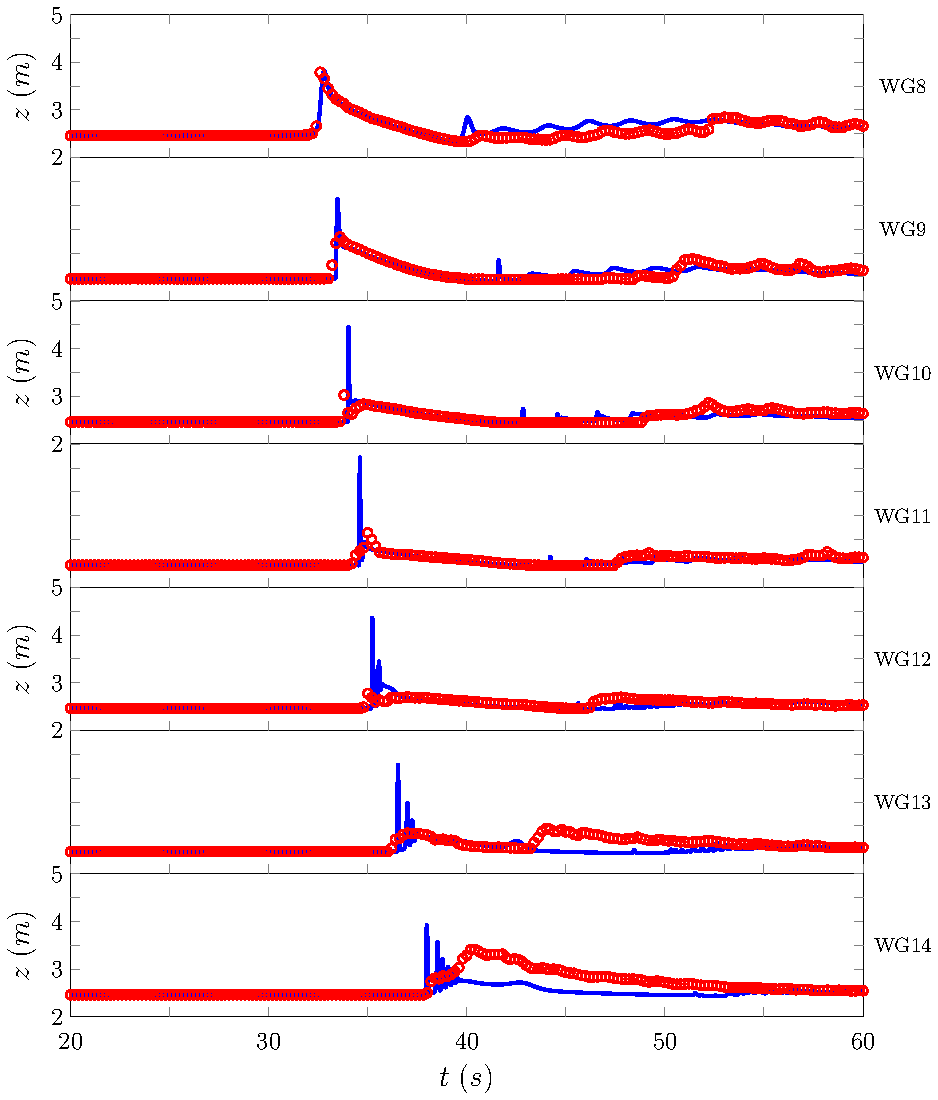
\includegraphics[width=\textwidth]{./chp6/figures/Experiment/Roeber/Trial8/FEVM/LongWGs2.pdf}
	\caption{Comparison of the experimental (\circlet{red}) and numerical ({\color{blue}\solidrule}) wave gauge data produced by $\text{FEVM}_2$ for gauges $6$ to $10$.}
	\label{fig:Roeber8WG6to10FEVM}
\end{figure}  
\begin{figure}
	\centering
	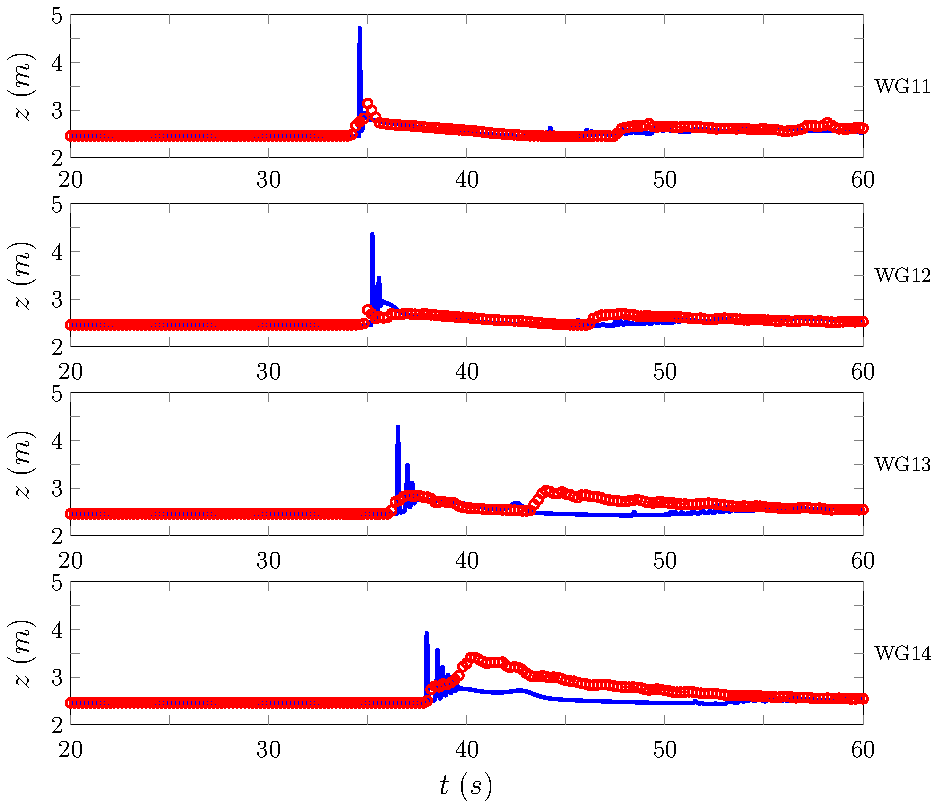
\includegraphics[width=\textwidth]{./chp6/figures/Experiment/Roeber/Trial8/FEVM/LongWGs3.pdf}
	\caption{Comparison of the experimental (\circlet{red}) and numerical ({\color{blue}\solidrule}) wave gauge data produced by $\text{FEVM}_2$ for gauges $11$ to $14$.}
	\label{fig:Roeber8WG11to14FEVM}
\end{figure}         
\begin{figure}
	\centering
	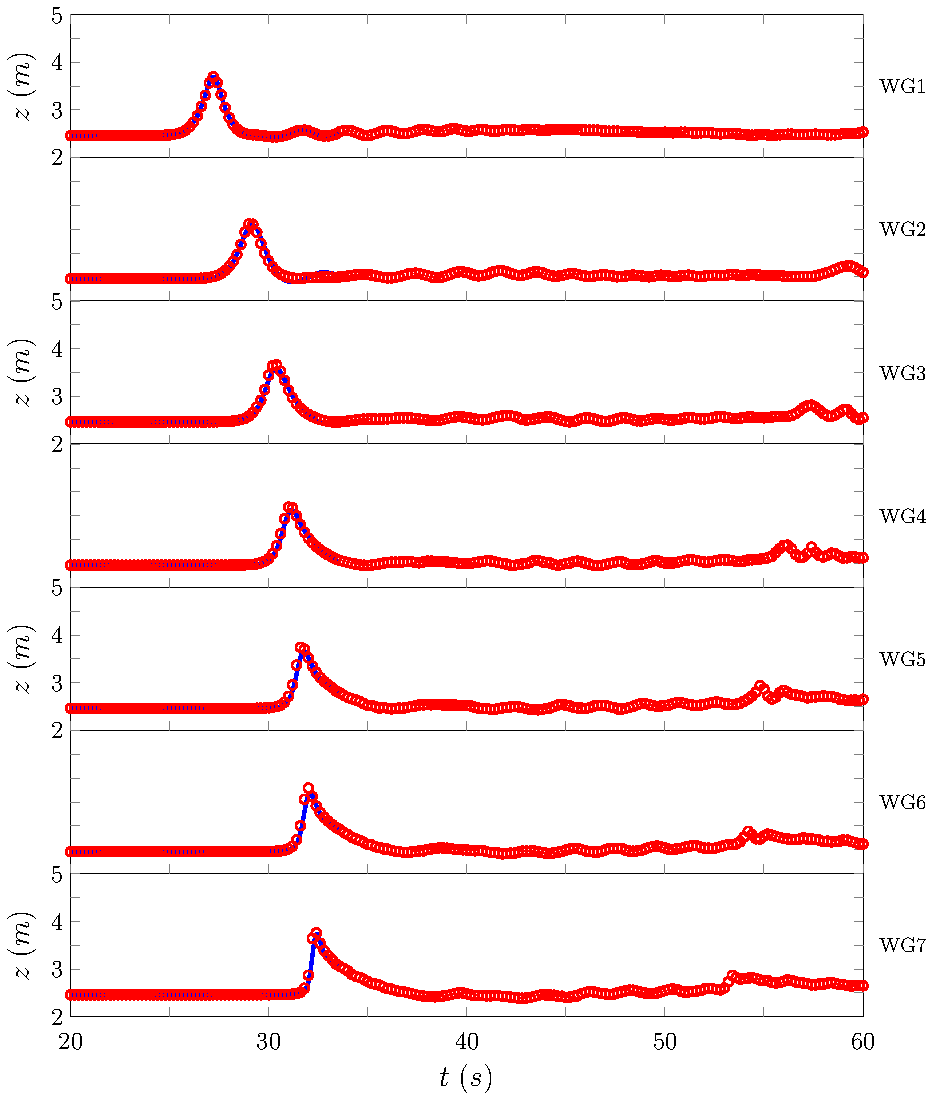
\includegraphics[width=\textwidth]{./chp6/figures/Experiment/Roeber/Trial8/FDVM/LongWGs1.pdf}
	\caption{Comparison of the experimental (\circlet{red}) and numerical ({\color{blue}\solidrule}) wave gauge data produced by $\text{FDVM}_2$ for gauges $1$ to $7$.}
	\label{fig:Roeber8WG1to5FDVM}
\end{figure}
\begin{figure}
	\centering
	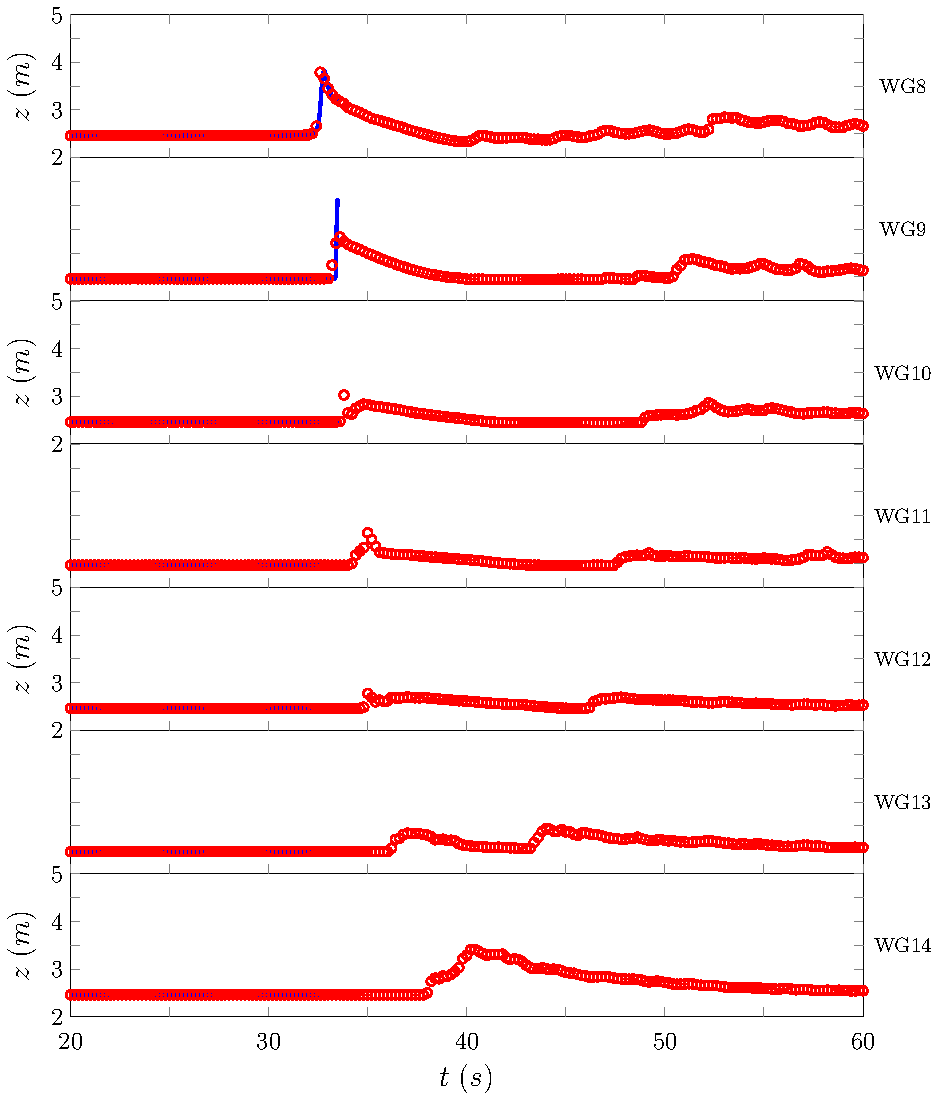
\includegraphics[width=\textwidth]{./chp6/figures/Experiment/Roeber/Trial8/FDVM/LongWGs2.pdf}
	\caption{Comparison of the experimental (\circlet{red}) and numerical ({\color{blue}\solidrule}) wave gauge data produced by $\text{FDVM}_2$ for gauges $6$ to $9$.}
	\label{fig:Roeber8WG6to9FDVM}
\end{figure} 

Both methods accurately reproduce the shoaling of the solitary wave, particularly in wave gauges $1$ through $8$ which record the wave before breaking begins. The behaviour of the trailing waves is not as well replicated, with the numerical solutions overestimating their amplitude and speed as in the previous experiments. The reflected wave can also be observed in the wave gauges and since the numerical simulation did not have reflective boundaries these waves are not replicated in their solution.

When breaking begins the numerical solutions perform much worse as expected; most notably $\text{FDVM}_2$ becomes unstable and the solution blows up. Because of this the numerical solution of $\text{FDVM}_2$ was only plotted until $t = 34s$. The instability is caused by the appearance of a very steep gradient with a large jump in the water depth compared to the depth of water that surrounds it as the wave breaks. The $\text{FEVM}_2$ method does not suffer from these instability issues, but due to the limitations of the Serre equations does produce a dispersive wave train with amplitudes far exceeding the observed amplitudes of the experiment. 

Given the limitations of the underlying Serre equations the results for $\text{FEVM}_2$ are robust and accurately model the shoaling of the solitary wave. However, these results indicate the need for more accurate handling of breaking waves to be able to accurately model physical situations. 

\section{Runup of a Solitary Wave on a Linearly Sloped Beach}
To study the run-up of incoming waves on linear beaches a series of experiments were conducted by \citet{Synolakis-1987-523}. These experiments consisted of a number of runup events for a wide array of breaking and non-breaking waves where snapshots of the entire water surface were taken at certain times. These experiments were all performed on the beach profile depicted in Figure \ref{fig:SynolakisWT}, where all the quantities are normalised \cite{Synolakis-1987-523}. To assess the computational models we recreated one of these experiments, which captured the runup of a non breaking solitary wave with a nonlinearity parameter of $\epsilon = 0.0185$.
\begin{figure}
	\centering
	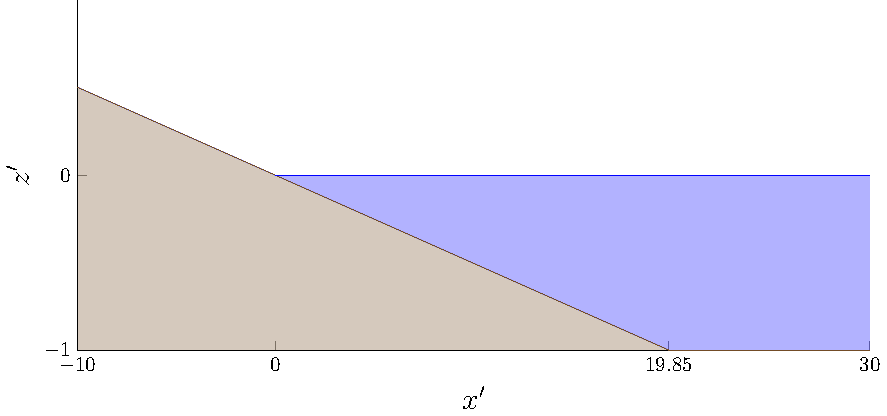
\includegraphics[width=\textwidth]{./chp6/figures/Experiment/Synolakis/WavetankArtifical.pdf}
	\caption{Diagram demonstrating the water (\squareF{blue}) and the ground  (\squareF{brown!80!black}) for the Synolakis experiment with the normalised coordinates.}
	\label{fig:SynolakisWT}
\end{figure}

This experiment allows us to compare the inundation behaviour of our numerical methods with experimental results. For this experiment the effect of dispersion on the run-up behaviour is minimal, and there is good agreement between numerical solutions of the SWWE and this particular experiment \cite{Bollermann-etal-2011-271}. Therefore, the effect of the extra dispersive terms included by the Serre equations on the inundation process is not well tested by this experiment, but it does demonstrate robustness. 

The numerical experiments used the normalised quantities reported by \citet{Synolakis-1987-523} to reproduce the experiment. The spatial domain was $x' \in [-30,150]$ with a resolution of $\Delta x = 0.05$ and was run until $t' = 70$ with the CFL condition \eqref{eqn:CFLcond} satisfied by setting $\Delta t = 0.1 \Delta x$. The spatial reconstruction used the input parameter $\theta = 1.2$ and gravity was normalised to match the coordinates and so $g= 1$.

\subsection{Results}

%Par 1: Figures

%Par 2: Discussion

%Par 3: Conclusion

The normalised water surface data is given at the various times in Figure \ref{fig:SynolakisFDVMNoBreak} for $\text{FDVM}_2$ and \ref{fig:SynolakisFEVMNoBreak} for $\text{FEVM}_2$. The error in conservation of the conserved quantities are given in Tables \ref{tab:ConservationSynFEVM} and \ref{tab:ConservationSynFDVM} for $\text{FEVM}_2$ and $\text{FDVM}_2$ respectively. 

\begin{figure}
	\centering
	\begin{subfigure}{0.5\textwidth}
		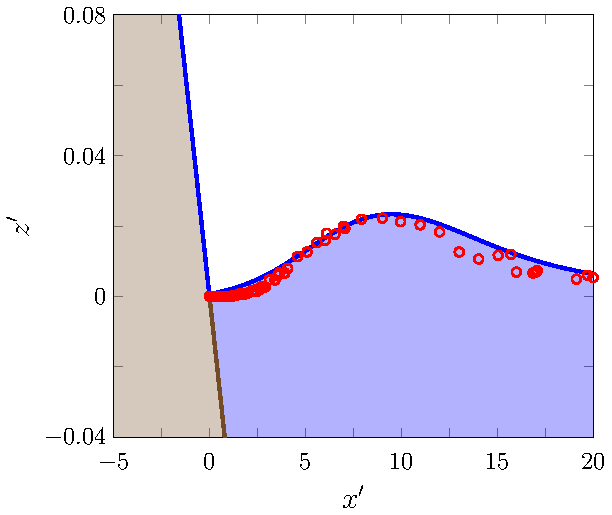
\includegraphics[width=\textwidth]{./chp6/figures/Experiment/Synolakis/H0p0185/FEVM/30s.pdf}
		\subcaption{$t'=30$}
		\vspace{0.5cm}
	\end{subfigure}%
	\begin{subfigure}{0.5\textwidth}
		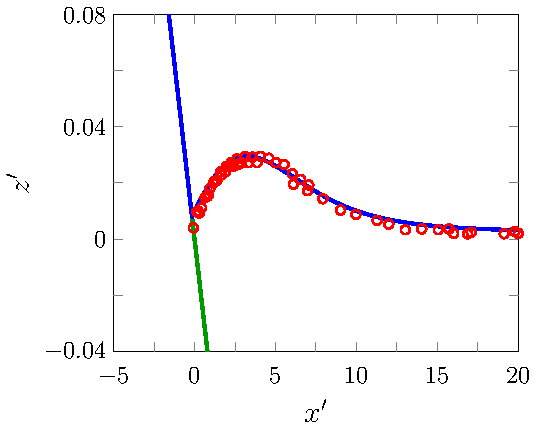
\includegraphics[width=\textwidth]{./chp6/figures/Experiment/Synolakis/H0p0185/FEVM/40s.pdf}
		\subcaption{$t'=40$}
		\vspace{0.5cm}
	\end{subfigure}
	\begin{subfigure}{0.5\textwidth}
		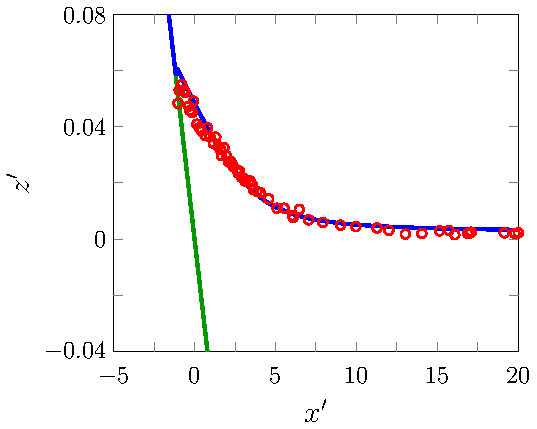
\includegraphics[width=\textwidth]{./chp6/figures/Experiment/Synolakis/H0p0185/FEVM/50s.pdf}
		\subcaption{$t'=50$}
		\vspace{0.5cm}
	\end{subfigure}%
	\begin{subfigure}{0.5\textwidth}
		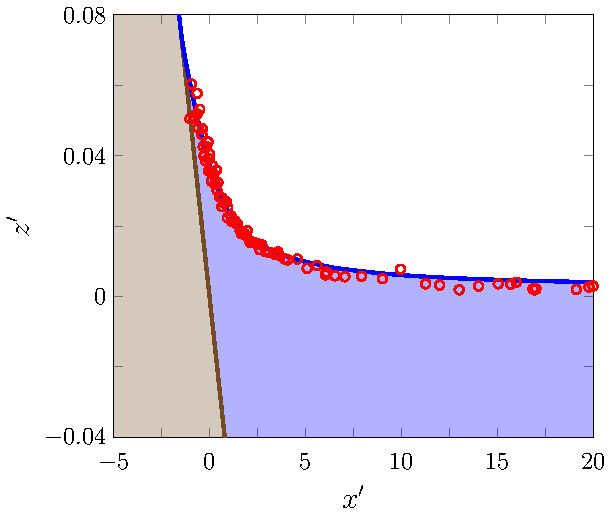
\includegraphics[width=\textwidth]{./chp6/figures/Experiment/Synolakis/H0p0185/FEVM/60s.pdf}
		\subcaption{$t'=60$}
		\vspace{0.5cm}
	\end{subfigure}
	\begin{subfigure}{0.5\textwidth}
		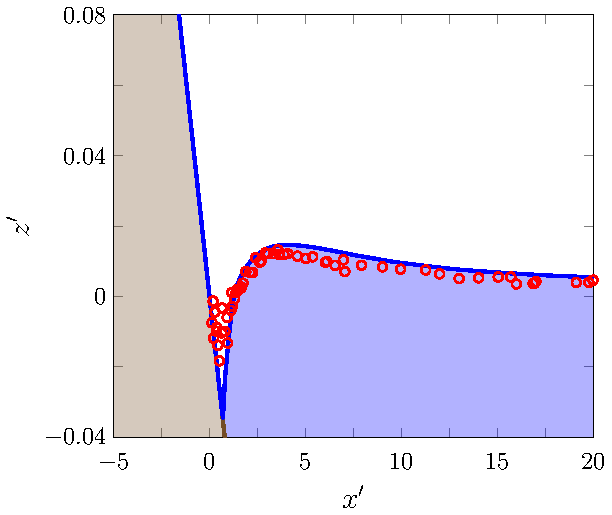
\includegraphics[width=\textwidth]{./chp6/figures/Experiment/Synolakis/H0p0185/FEVM/70s.pdf}
		\subcaption{$t'=70$}
		\vspace{0.5cm}
	\end{subfigure}
	\caption{A comparison of the water surface profiles for the experiment (\circlet{red}) and the numerical solution ({\color{blue}\solidrule}) produced by $\text{FEVM}_2$ at various times.}
	\label{fig:SynolakisFEVMNoBreak}
\end{figure}
\begin{figure}
	\centering
	\begin{subfigure}{0.5\textwidth}
		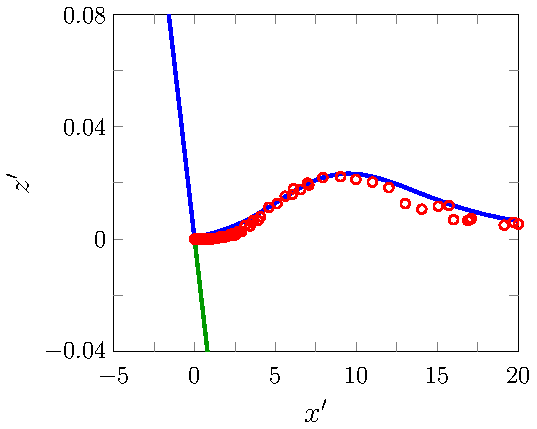
\includegraphics[width=\textwidth]{./chp6/figures/Experiment/Synolakis/H0p0185/FDVM/30s.pdf}
		\subcaption{$t'=30$}
		\vspace{0.5cm}
	\end{subfigure}%
	\begin{subfigure}{0.5\textwidth}
		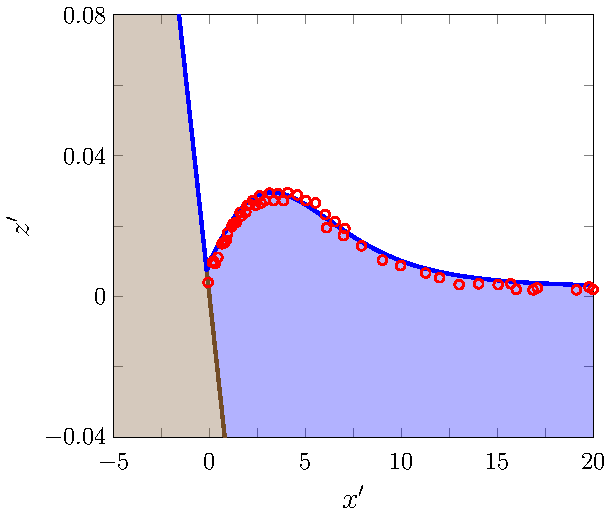
\includegraphics[width=\textwidth]{./chp6/figures/Experiment/Synolakis/H0p0185/FDVM/40s.pdf}
		\subcaption{$t'=40$}
		\vspace{0.5cm}
	\end{subfigure}
	\begin{subfigure}{0.5\textwidth}
		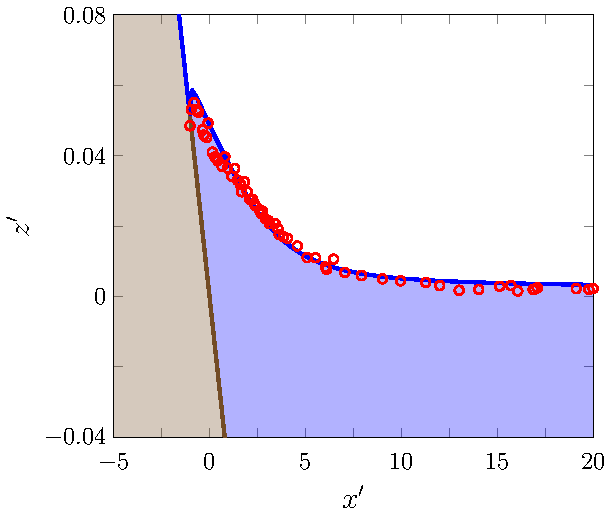
\includegraphics[width=\textwidth]{./chp6/figures/Experiment/Synolakis/H0p0185/FDVM/50s.pdf}
		\subcaption{$t'=50$}
		\vspace{0.5cm}
	\end{subfigure}%
	\begin{subfigure}{0.5\textwidth}
		\includegraphics[width=\textwidth]{./chp6/figures/Experiment/Synolakis/H0p0185/FDVM/60s.pdf}
		\subcaption{$t'=60$}
		\vspace{0.5cm}
	\end{subfigure}
	\begin{subfigure}{0.5\textwidth}
		\includegraphics[width=\textwidth]{./chp6/figures/Experiment/Synolakis/H0p0185/FDVM/70s.pdf}
		\subcaption{$t'=70$}
		\vspace{0.5cm}
	\end{subfigure}
	\caption{A comparison of the water surface profiles for the experiment (\circlet{red}) and the numerical solution ({\color{blue}\solidrule}) produced by $\text{FDVM}_2$ at various times.}
	\label{fig:SynolakisFDVMNoBreak}
\end{figure}

Both methods reproduce the experimental results very well, replicating the incoming wave properties and the maximum runup very well. The experimental wave appears to be more skewed towards the shoreline, but this shape difference has all but disappeared as the wave begins to inundate the shore. The only other noticeable difference is that the numerical solutions appear to run down further than the experimental results. The observed larger rundown is likely caused by the lack of friction in the Serre equations.

%make sure its understandable
The conserved quantities are well conserved by the method throughout the run up and rundown of the wave, particularly the mass. The total energy of the method is also well conserved, however the energy appears to have slightly increased in the method during the run-up process due to the handling of the dry bed problem. During this experiment kinetic energy is converted into gravitational potential energy and then back again as the wave is reflected, therefore $uh$ and $G$ will only be conserved in this experiment after the wave has completely reflected from the beach. Full reflection of the wave has not occurred by $t'=70s$ and so the conservation results for $uh$ and $G$ were omitted from Tables \ref{tab:ConservationSynFEVM} and \ref{tab:ConservationSynFDVM}.

The results for both $\text{FEVM}_2$ and $\text{FDVM}_2$ are identical in these Figures as these grids are quite fine and so these figures represent a good approximation to the true solution of the Serre equations. These numerical solutions demonstrate good agreement with experimental results and display the capability of the method to model the inundation of non-breaking waves.

%Negative energy
\begin{table}
	\centering
	\begin{tabular}{l  c  c c}
		Quantity& $\mathcal{C}^*\left(\vecn{q}^0\right)$ & $\mathcal{C}^*\left(\vecn{q}^*\right)$ & $\mathcal{C}^*_1\left(\vecn{q}^0,\vecn{q}^*\right)$  \B\\
		\hline 
		$h$ & $140.4170$ & $140.4170$ & $7.65\times 10^{-12}$ \T \\
		%$uh$ & $-0.3191$ & $0.3203$ & $0.0040$\\
		%$G$ & $-0.3191$ & $0.3204$ & $0.0043$\\
		$\mathcal{H}$ & $68.3900$ & $68.3914$ & $2.16 \times 10^{-5}$ \B\\
		\hline
	\end{tabular}
	\caption{Initial and final total amounts and the conservation error for all conserved quantities for $\text{FEVM}_2$'s numerical solution of the runup experiment.}
	\label{tab:ConservationSynFEVM}
\end{table}

\begin{table}
	\centering
	\begin{tabular}{l  c  c c}
		Quantity& $\mathcal{C}^*\left(\vecn{q}^0\right)$ & $\mathcal{C}^*\left(\vecn{q}^*\right)$ & $\mathcal{C}^*_1\left(\vecn{q}^0,\vecn{q}^*\right)$ \B \\
		\hline
		$h$ & $140.4170$ & $140.4170$ & $1.11\times 10^{-7}$ \T\\
		%$uh$ & $-0.3191$ & $0.3196$ & $0.0017$\\
		%$G$ & $-0.3191$ & $0.3207$ & $0.0050$\\
		$\mathcal{H}$ & $68.3900$ & $68.3914$ & $2.16 \times 10^{-5}$ \B \\
		\hline
	\end{tabular}
	\caption{Initial and final total amounts and the conservation error for all conserved quantities for $\text{FDVM}_2$'s numerical solution of the runup experiment.}
	\label{tab:ConservationSynFDVM}
\end{table}

\medskip

In this chapter $\text{FEVM}_2$ and $\text{FDVM}_2$ were validated using experimental data. It was found that for most experiments the solutions of $\text{FEVM}_2$ and $\text{FDVM}_2$ were identical although $\text{FEVM}_2$ is the preferred method due to its greater robustness. 


  
\chapter{Experimental Validation}
\label{chp:ExpMethodComp}
In this chapter the second-order hybrid finite volume methods are assessed using experimental data. 

The numerical methods $\text{FDVM}_2$ and $\text{FEVM}_2$ are experimentally validated by comparing their numerical solutions to experimental data. The chosen experiments allow the methods capability to model a variety of physical situations to be tested. These situations include the presence of steep gradients in the flow, the interaction of strong dispersive waves with varying bathymetry, shoaling and wave breaking and finally the wetting and drying of a beach. Thus, the ability of these methods to reproduce all the experimental results well strongly demonstrates their capability to model all physical situations very well. 

\section{Evolution of Rectangular Depression}
A series of experiments studying the evolution of rectangular depressions and thus steep gradients in the free-surface was conducted by \citet{Hammack-Segur-1978-337}. These experiments were performed in a wave tank that was $0.394m$ wide, $31.6m$ long and $0.61m$ high. The rectangular depressions were generated using a piston $0.61m$ long with its left edge against the wave tank wall. The $0.1m$ deep water is initially stationary with a horizontal free surface and the piston in the up position. The experiment begins when the piston suddenly moves down. This creates a sudden depression in the water surface, generating waves that are recorded at wave gauges located at $0m$, $5m$, $10m$, $15m$ and $20m$ from the right edge of the piston. A diagram of the longitudinal section of the wave-tank with the wave gauge locations is given in Figure \ref{fig:SegurWT}.

\begin{figure}
	\centering
	\includegraphics[width=\textwidth]{./chp6/figures/Experiment/Segur/WaveTank.pdf}
	\caption{Diagram demonstrating the water (\squareF{blue}) and the bed (\squareF{brown!80!black}) for the Segur experiments, with the wave gauge locations marked.}
	\label{fig:SegurWT}
\end{figure} 

These experiments provide a good benchmark for the capability of the numerical method to accurately model problems with steep gradients in the free surface. These experiments are affected by bed friction and viscosity and the inability of the piston and water to move vertically instantaneously. Since the Serre equations do not contain viscosity, bed friction and we use discontinuous initial conditions we expect numerical solutions of the Serre equations to produce many more oscillations in  the dispersive wave trains than are observed experimentally \cite{Pitt-2018-61}.

\citet{Hammack-Segur-1978-337} report the results for two different initial depression depths $0.01m$ and $0.03m$, resulting in the nonlinearity parameters $\epsilon = 0.1$ and $\epsilon=0.3$ respectively. Since these nonlinearity parameters are relatively small there was no breaking of waves throughout the experiment. 

This experiment was modelled numerically using the reflected problem, with the wall as the axis of symmetry. In the numerical experiments the domain is $[-60m,60m]$ and the experiment is run for $ 50s$ with $g = 9.81m/s^2$. For the spatial resolution we set $\Delta x = 0.01m$ to satisfy the CFL condition, \eqref{eqn:CFLcond} $\Delta t = 0.5 \Delta x / \sqrt{g \; 0.1}$. The limiting parameter $\theta = 1.2$ was used in the reconstruction in $\text{FEVM}_2$ and $\text{FDVM}_2$.

\subsection{Results for $0.01m$ Rectangular Depression}

Plots comparing the numerical and experimental wave gauge data for the $0.01m$ rectangular depression are displayed in Figures \ref{fig:Segur1cmFEVM} and \ref{fig:Segur1cmFDVM} for $\text{FEVM}_2$ and $\text{FDVM}_2$ respectively. We present this data using the same dimensionless scales as reported in the original paper \cite{Hammack-Segur-1978-337}. Tables \ref{tab:ConservationSegurFEVM1cm} and \ref{tab:ConservationSegurFDVM1cm} are also provided, which record the conservation of all the quantities. 
\begin{figure}
	\centering
	\includegraphics[width=\textwidth]{./chp6/figures/Experiment/Segur/LongWGsFEVM1cm.pdf}
	\caption{Comparison of experimental wave gauge data ({\color{red}\solidrule}) and numerical results ({\color{blue}\solidrule}) of $\text{FEVM}_2$ for the $0.01m$ rectangular depression.}
	\label{fig:Segur1cmFEVM}
\end{figure}
\begin{figure}
	\centering
	\includegraphics[width=\textwidth]{./chp6/figures/Experiment/Segur/LongWGsFDVM1cm.pdf}
	\caption{FDVM}
	\caption{Comparison of experimental wave gauge data ({\color{red}\solidrule}) and numerical results ({\color{blue}\solidrule}) of $\text{FDVM}_2$ for the $0.01m$ rectangular depression.}
	\label{fig:Segur1cmFDVM}
\end{figure} 

The numerical solutions agree well with the experimental results; particularly for the front of the dispersive wave train. While all the conserved quantities have indeed been conserved very well by the methods.  

The numerical solutions produce larger and consequently faster waves and observe oscillations in the depression which are not observed in the experimental data of wave gauge $1$. Moreover, as expected the methods produce many more oscillations than were observed experimentally. These discrepancies can be attributed to the lack of viscosity and bed friction in the Serre equations \eqref{eqn:FullSerreCon}. Furthermore, it is highly likely the experiment produced some smooth approximation to a discontinuous jump in the water depth with the down-stroke of the piston. Such a smoothing of the initial conditions will significantly attenuate the higher frequency waves in the generated dispersive wave train \cite{Pitt-2018-61}. Given these challenges the numerical methods do a very good job of replicating the experimental behaviour. 

Both $\text{FEVM}_2$ and $\text{FDVM}_2$ have produced visually identical results at this scale and have demonstrated very good conservation of all the quantities see, Tables \ref{tab:ConservationSegurFEVM1cm} and \ref{tab:ConservationSegurFDVM1cm}. Given the extensive review of these methods \cite{Pitt-2018-61} for steep gradient problems, this indicates that these solutions are indicative of true solutions of the Serre equations which are capable of reproducing experimental results.
%
\begin{table}
	\centering
	\begin{tabular}{l  c  c c}
		Quantity& $\mathcal{C}^*\left(\vecn{q}^0\right)$ & $\mathcal{C}^*\left(\vecn{q}^*\right)$ & $\mathcal{C}^*_1\left(\vecn{q}^0,\vecn{q}^*\right)$  \B\\
		\hline
		$h$ & $11.9888$ & $11.9888$ & $0$ \T\\
		$uh$ & $0$ & $7.44 \times 10^{-18}$ & $7.44 \times 10^{-18}$\\
		$G$ & $0$ & $1.56\times 10^{-18}$ & $1.56\times 10^{-18}$\\
		$\mathcal{H}$ & $5.8751$ & $5.8751$ & $5.70 \times 10^{-6}$ \B \\
		\hline
	\end{tabular}
	\caption{Initial and final total amounts and the conservation error for all conserved quantities for $\text{FEVM}_2$ numerical solution of the $0.01m$ rectangular depression.}
	\label{tab:ConservationSegurFEVM1cm}
\end{table} 
%
\begin{table}
	\centering
	\begin{tabular}{l  c  c c}
		Quantity& $\mathcal{C}^*\left(\vecn{q}^0\right)$ & $\mathcal{C}^*\left(\vecn{q}^*\right)$ & $\mathcal{C}^*_1\left(\vecn{q}^0,\vecn{q}^*\right)$ \B \\
		\hline
		$h$ & $11.9888$ & $11.9888$ & $0$ \T\\
		$uh$ & $0$ & $-1.19 \times 10^{-17}$ & $-1.19 \times 10^{-17}$\\
		$G$ & $0$ & $-8.05\times 10^{-18}$ & $-8.05\times 10^{-18}$\\
		$\mathcal{H}$ & $5.8751$ & $5.8751$ & $6.27 \times 10^{-6}$ \B\\
		\hline
	\end{tabular}
	\caption{Initial and final total amounts and the conservation error for all conserved quantities for $\text{FDVM}_2$ numerical solution of the $0.01m$ rectangular depression.}
	\label{tab:ConservationSegurFDVM1cm}
\end{table}  
 

\subsection{Results for $0.03m$ Rectangular Depression}
The wave gauge data for the numerical and experimental results for the evolution of the $0.03m$ rectangular depression are displayed in Figures \ref{fig:Segur3cmFEVM} and \ref{fig:Segur3cmFDVM} for $\text{FEVM}_2$ and $\text{FDVM}_2$ respectively. These results are reported using the same dimensionless scales as the original paper \cite{Hammack-Segur-1978-337}. The conservation of all the conserved quantities are given in Tables \ref{tab:ConservationSegurFEVM3cm} and \ref{tab:ConservationSegurFEVM3cm} for $\text{FEVM}_2$ and $\text{FDVM}_2$ respectively.
\begin{figure}
	\centering
	\includegraphics[width=\textwidth]{./chp6/figures/Experiment/Segur/LongWGsFEVM3cm.pdf}
	\caption{Comparison of experimental wave gauge data ({\color{red}\solidrule}) and numerical results ({\color{blue}\solidrule}) of $\text{FEVM}_2$ for the $0.03m$ rectangular depression.}
	\label{fig:Segur3cmFEVM}
\end{figure}
\begin{figure}
	\centering
	\includegraphics[width=\textwidth]{./chp6/figures/Experiment/Segur/LongWGsFDVM3cm.pdf}
	\caption{Comparison of experimental wave gauge data ({\color{red}\solidrule}) and numerical results ({\color{blue}\solidrule}) of $\text{FDVM}_2$ for the $0.03m$ rectangular depression.}
	\label{fig:Segur3cmFDVM}
\end{figure} 

Both methods again reproduce the overall behaviour of this experiment very well. Because the rectangular wave is deeper, this experiment provides a more rigorous test for the numerical methods. However, increasing the depth also strengthens the causes of the discrepancy between the experimental results and the numerical solutions of the Serre equations. This can be seen most acutely for the amplitude and speed of the generated waves.

Since the rectangular depression is larger the numerical methods have a larger error in conservation for all the quantities as compared to the $0.01m$ rectangular depression except mass; which is conserved exactly. For $G$ and momentum these errors are around machine epsilon and can be disregarded, so that only the conservation of energy is significantly effected. Even with this larger error, all quantities are still well conserved by the numerical methods, suggesting that the numerical solutions well approximate the true solutions of the Serre equations. 

These experiments have been well replicated by the numerical methods, and given the resolution and error in conservation and the extensive study summarised in Chapter \ref{chp:Serreeqns}; these results demonstrate the accuracy of the numerical methods in the presence of steep gradients in the free surface.       
%
\begin{table}
	\centering
	\begin{tabular}{l  c  c c}
		Quantity& $\mathcal{C}^*\left(\vecn{q}^0\right)$ & $\mathcal{C}^*\left(\vecn{q}^*\right)$ & $\mathcal{C}^*_1\left(\vecn{q}^0,\vecn{q}^*\right)$ \B \\
		\hline 
		$h$ & $11.9644$ & $11.9644$ & $0$ \T\\
		$uh$ & $0$ & $-7.75 \times 10^{-17}$ & $-7.75\times 10^{-17}$\\
		$G$ & $0$ & $-3.33\times 10^{-16}$ & $-3.33\times 10^{-16}$\\
		$\mathcal{H}$ & $5.8560$ & $5.8552$ & $1.24 \times 10^{-4}$  \B \\
		\hline
	\end{tabular}
	\caption{Initial and final total amounts and the conservation error for all conserved quantities for $\text{FEVM}_2$ numerical solution of the $0.03m$ rectangular depression.}
	\label{tab:ConservationSegurFEVM3cm}
\end{table} 
%
\begin{table}
	\centering
	\begin{tabular}{l  c  c c}
		Quantity& $\mathcal{C}^*\left(\vecn{q}^0\right)$ & $\mathcal{C}^*\left(\vecn{q}^*\right)$ & $\mathcal{C}^*_1\left(\vecn{q}^0,\vecn{q}^*\right)$ \B \\
		\hline
		$h$ & $11.9644$ & $11.9644$ & $0$ \T\\
		$uh$ & $0$ & $-9.09 \times 10^{-17}$ & $-9.09 \times 10^{-17}$\\
		$G$ & $0$ & $-1.16\times 10^{-16}$ & $-1.16\times 10^{-16}$\\
		$\mathcal{H}$ & $5.8560$ & $5.8552$ & $1.30 \times 10^{-4}$ \B\\
		\hline
	\end{tabular}
	\caption{Initial and final total amounts and the conservation error for all conserved quantities for $\text{FDVM}_2$ numerical solution of the $0.03m$ rectangular depression.}
	\label{tab:ConservationSegurFDVM3cm}
\end{table}  

\section{Periodic Waves Over A Submerged Bar}
\label{sec:PeriodicWavessubBar}
Beji and Battjes conducted a series of experiments investigating the effect of submerged bars on the propagation of periodic waves \cite{Beji-Battjes-1993-151,Beji-Battjes-1994-1}. The behaviour of these experiments were mainly driven by the dispersion properties of the waves and their interaction with variations in bathymetry. Therefore, these experiments serve as a benchmark for the ability of the numerical schemes to accurately model the interaction of variable bathymetry and dispersive waves. For our purposes we will focus on the monochromatic wave experiments of \citet{Beji-Battjes-1994-1}.

The experiments of \citet{Beji-Battjes-1994-1} were conducted in a wave tank $37.7m$ long, $0.8m$ wide and $0.75m$ high. A diagram of the longitudinal section of the wave tank is given in Figure \ref{fig:BejiWT}. There are seven wave gauges at the following locations; $5.7m$, $10.5m$, $12.5m$, $13.5m$, $14.5m$, $15.7m$ and $17.3m$. Waves are generated from a piston-type wave maker located at $0m$ and travel on the initially still water $0.4m$ deep to the right, over the submerged trapezoidal bar and are absorbed by a sloping beach.
\begin{figure}
	\centering
	\includegraphics[width=\textwidth]{./chp6/figures/Experiment/Beji/BejiTank.pdf}
	\caption{The flume configuration with water (\squareF{blue}) and the bed (\squareF{brown!80!black}) for the Beji experiments, with the wave gauge locations marked.}
	\label{fig:BejiWT}
\end{figure}

Two sinusoidal monochromatic non-breaking wave experiments were conducted. A low frequency one with a wavelength $\lambda \approx 3.69m$ and a period of $T = 2s$, and a high frequency one with $\lambda \approx 2.05m$ and a period of $T = 1.25s$. Both experiments had a wave amplitude of $0.01m$ and so both had the same small non-linearity parameter $\epsilon = 0.01 / 0.4 = 0.025$. 

We numerically simulated these experiments over the spatial domain $\left[5.7m,150m\right]$ with $\Delta x = 0.1 / 2^4 m \approx 0.0063m$ and $\Delta t = Sp / 2^5 s \approx 0.0012s$ where $Sp = 0.039 s$ is the experimental sampling period. These $\Delta x$ and $\Delta t$ values satisfy the CFL condition, \eqref{eqn:CFLcond}. In our numerical experiments only the submerged trapezoidal bar is present, and the sloping beach is replaced with a very long horizontal bed that ensures that we do not observe any effects from the Dirichlet boundary conditions at the downstream boundary.  

To simulate the incoming waves at the upstream boundary we used the first wave gauge as our left boundary condition together with linear extrapolation to calculate the other required $h$ values in the left ghost cell. The velocity boundary conditions were calculated from the height values in the same way as \citet{Beji-Battjes-1994-1}
\begin{equation*}
u(x,t) = \sqrt{g h_0} \; \dfrac{h(x,t) - h_0}{h(x,t)}.
\end{equation*}
Finally the boundary conditions for $G$ were calculated using the boundary conditions for $h$ and $u$. 

We shall now present our numerical results for the low and high frequency experiments.
%
\subsection{Low Frequency Results}
A comparison of the wave heights $\eta$ of the experimental and numerical results are located in Figures \ref{fig:BejislWG1to4FEVM} and \ref{fig:BejislWG5to7FEVM} for $\text{FEVM}_2$ and Figures \ref{fig:BejislWG1to4FDVM} and \ref{fig:BejislWG5to7FDVM} for $\text{FDVM}_2$. These numerical schemes both produce identical results for all wave gauges and so this benchmark does not help us discriminate between these two methods. 
\begin{figure}
	\centering
	\begin{subfigure}{0.5\textwidth}
		\includegraphics[width=\textwidth]{./chp6/figures/Experiment/Beji/sl/FEVMWG1.pdf}
		\subcaption{Wave Gauge $1$}
		\vspace{0.5cm}
	\end{subfigure}%
	\begin{subfigure}{0.5\textwidth}
		\includegraphics[width=\textwidth]{./chp6/figures/Experiment/Beji/sl/FEVMWG2.pdf}
		\subcaption{Wave Gauge $2$}
		\vspace{0.5cm}
	\end{subfigure}
	\begin{subfigure}{0.5\textwidth}
		\includegraphics[width=\textwidth]{./chp6/figures/Experiment/Beji/sl/FEVMWG3.pdf}
		\subcaption{Wave Gauge $3$}
		\vspace{0.5cm}
	\end{subfigure}%
	\begin{subfigure}{0.5\textwidth}
		\includegraphics[width=\textwidth]{./chp6/figures/Experiment/Beji/sl/FEVMWG4.pdf}
		\subcaption{Wave Gauge $4$}
		\vspace{0.5cm}
	\end{subfigure}
	\caption{Comparison of the wave heights $\eta$ of the numerical results for the $\text{FEVM}_2$ ({\color{blue}\solidrule}) and the experimental results (\circlet{red}) for wave gauges $1$ - $4$ for the low frequency experiment.}
	\label{fig:BejislWG1to4FEVM}
\end{figure}
%
\begin{figure}
	\centering
	\begin{subfigure}{0.5\textwidth}
		\includegraphics[width=\textwidth]{./chp6/figures/Experiment/Beji/sl/FEVMWG5.pdf}
		\subcaption{Wave Gauge $5$}
		\vspace{0.5cm}
	\end{subfigure}%
	\begin{subfigure}{0.5\textwidth}
		\includegraphics[width=\textwidth]{./chp6/figures/Experiment/Beji/sl/FEVMWG6.pdf}
		\subcaption{Wave Gauge $6$}
		\vspace{0.5cm}
	\end{subfigure}
	\begin{subfigure}{0.5\textwidth}
		\includegraphics[width=\textwidth]{./chp6/figures/Experiment/Beji/sl/FEVMWG7.pdf}
		\subcaption{Wave Gauge $7$}
		\vspace{0.5cm}
	\end{subfigure}
	\caption{Comparison of the wave heights $\eta$ of the numerical results for the $\text{FEVM}_2$ ({\color{blue}\solidrule}) and the experimental results (\circlet{red}) for wave gauges $5$ - $7$ for the low frequency experiment.}
	\label{fig:BejislWG5to7FEVM}
\end{figure}
%
\begin{figure}
	\centering
	\begin{subfigure}{0.5\textwidth}
		\includegraphics[width=\textwidth]{./chp6/figures/Experiment/Beji/sl/FDVMWG1.pdf}
		\subcaption{Wave Gauge $1$}
		\vspace{0.5cm}
	\end{subfigure}%
	\begin{subfigure}{0.5\textwidth}
		\includegraphics[width=\textwidth]{./chp6/figures/Experiment/Beji/sl/FDVMWG2.pdf}
		\subcaption{Wave Gauge $2$}
		\vspace{0.5cm}
	\end{subfigure}
	\begin{subfigure}{0.5\textwidth}
		\includegraphics[width=\textwidth]{./chp6/figures/Experiment/Beji/sl/FDVMWG3.pdf}
		\subcaption{Wave Gauge $3$}
		\vspace{0.5cm}
	\end{subfigure}%
	\begin{subfigure}{0.5\textwidth}
		\includegraphics[width=\textwidth]{./chp6/figures/Experiment/Beji/sl/FDVMWG4.pdf}
		\subcaption{Wave Gauge $4$}
		\vspace{0.5cm}
	\end{subfigure}
	\caption{Comparison of the wave heights $\eta$ of the numerical results for the $\text{FDVM}_2$ ({\color{blue}\solidrule}) and the experimental results (\circlet{red}) for wave gauges $1$ - $4$ for the low frequency experiment.}
	\label{fig:BejislWG1to4FDVM}
\end{figure}
%
\begin{figure}
	\centering
	\begin{subfigure}{0.5\textwidth}
		\includegraphics[width=\textwidth]{./chp6/figures/Experiment/Beji/sl/FDVMWG5.pdf}
		\subcaption{Wave Gauge $5$}
		\vspace{0.5cm}
	\end{subfigure}%
	\begin{subfigure}{0.5\textwidth}
		\includegraphics[width=\textwidth]{./chp6/figures/Experiment/Beji/sl/FDVMWG6.pdf}
		\subcaption{Wave Gauge $6$}
		\vspace{0.5cm}
	\end{subfigure}
	\begin{subfigure}{0.5\textwidth}
		\includegraphics[width=\textwidth]{./chp6/figures/Experiment/Beji/sl/FDVMWG7.pdf}
		\subcaption{Wave Gauge $7$}
		\vspace{0.5cm}
	\end{subfigure}
	\caption{Comparison of the wave heights $\eta$ of the numerical results for the $\text{FDVM}_2$ ({\color{blue}\solidrule}) and the experimental results (\circlet{red}) for wave gauges $5$ - $7$ for the low frequency experiment.}
	\label{fig:BejislWG5to7FDVM}
\end{figure}

These results demonstrate the ability of these numerical methods to recreate the experimental results, particularly for wave gauge $1$ to $5$ where the agreement between experimental and numerical results is best. Results at these gauges validate the numerical schemes for simulating shoaling of dispersive waves as these wave gauges are all located on the windward side of the submerged bar where shoaling occurs in the experiment. 

The numerical results for wave gauges $6$ and $7$ on the leeward side capture some of the wave behaviour but their agreement with the experiments results is much worse. The inadequacy of the numerical results here appears to be due to the discrepancy between the dispersion properties of the Serre equations and actual water waves \cite{Beji-Battjes-1994-1,Lannes-2013}.

The dispersion terms in the Serre equations are vital to recreating the experimental results for wave gauges $2$ to $5$, as non-dispersive equations such as the SWWE are not capable of accurately simulating this experiment \cite{Pitt-2017-1725}.

\subsection{High Frequency Results}
The wave heights of the experimental and numerical results are given in Figures \ref{fig:BejishWG1to4FEVM} and \ref{fig:BejishWG5to7FEVM} for $\text{FEVM}_2$. While the results for $\text{FDVM}_2$ are given in Figures \ref{fig:BejishWG1to4FDVM} and \ref{fig:BejishWG5to7FDVM}. As for the low frequency experiment $\text{FEVM}_2$ and $\text{FDVM}_2$ produce identical results for all wave gauges at this scale and so this benchmark does not discriminate between these two methods. 
%
\begin{figure}
	\centering
	\begin{subfigure}{0.5\textwidth}
		\includegraphics[width=\textwidth]{./chp6/figures/Experiment/Beji/sh/FEVMWG1.pdf}
		\subcaption{Wave Gauge $1$}
		\vspace{0.5cm}
	\end{subfigure}%
	\begin{subfigure}{0.5\textwidth}
		\includegraphics[width=\textwidth]{./chp6/figures/Experiment/Beji/sh/FEVMWG2.pdf}
		\subcaption{Wave Gauge $2$}
		\vspace{0.5cm}
	\end{subfigure}
	\begin{subfigure}{0.5\textwidth}
		\includegraphics[width=\textwidth]{./chp6/figures/Experiment/Beji/sh/FEVMWG3.pdf}
		\subcaption{Wave Gauge $3$}
		\vspace{0.5cm}
	\end{subfigure}%
	\begin{subfigure}{0.5\textwidth}
		\includegraphics[width=\textwidth]{./chp6/figures/Experiment/Beji/sh/FEVMWG4.pdf}
		\subcaption{Wave Gauge $4$}
		\vspace{0.5cm}
	\end{subfigure}
	\caption{Comparison of the wave heights $\eta$ of the numerical results for the $\text{FEVM}_2$ ({\color{blue}\solidrule}) and the experimental results (\circlet{red}) for wave gauges $1$ - $4$ for the low frequency experiment.}
	\label{fig:BejishWG1to4FEVM}
\end{figure}
%
\begin{figure}
	\centering
	\begin{subfigure}{0.5\textwidth}
		\includegraphics[width=\textwidth]{./chp6/figures/Experiment/Beji/sh/FEVMWG5.pdf}
		\subcaption{Wave Gauge $5$}
		\vspace{0.5cm}
	\end{subfigure}%
	\begin{subfigure}{0.5\textwidth}
		\includegraphics[width=\textwidth]{./chp6/figures/Experiment/Beji/sh/FEVMWG6.pdf}
		\subcaption{Wave Gauge $6$}
		\vspace{0.5cm}
	\end{subfigure}
	\begin{subfigure}{0.5\textwidth}
		\includegraphics[width=\textwidth]{./chp6/figures/Experiment/Beji/sh/FEVMWG7.pdf}
		\subcaption{Wave Gauge $7$}
		\vspace{0.5cm}
	\end{subfigure}
	\caption{Comparison of the wave heights $\eta$ of the numerical results for the $\text{FEVM}_2$ ({\color{blue}\solidrule}) and the experimental results (\circlet{red}) for wave gauges $5$ - $7$ for the high frequency experiment.}
	\label{fig:BejishWG5to7FEVM}
\end{figure}
%
\begin{figure}
	\centering
	\begin{subfigure}{0.5\textwidth}
		\includegraphics[width=\textwidth]{./chp6/figures/Experiment/Beji/sh/FDVMWG1.pdf}
		\subcaption{Wave Gauge $1$}
		\vspace{0.5cm}
	\end{subfigure}%
	\begin{subfigure}{0.5\textwidth}
		\includegraphics[width=\textwidth]{./chp6/figures/Experiment/Beji/sh/FDVMWG2.pdf}
		\subcaption{Wave Gauge $2$}
		\vspace{0.5cm}
	\end{subfigure}
	\begin{subfigure}{0.5\textwidth}
		\includegraphics[width=\textwidth]{./chp6/figures/Experiment/Beji/sh/FDVMWG3.pdf}
		\subcaption{Wave Gauge $3$}
		\vspace{0.5cm}
	\end{subfigure}%
	\begin{subfigure}{0.5\textwidth}
		\includegraphics[width=\textwidth]{./chp6/figures/Experiment/Beji/sh/FDVMWG4.pdf}
		\subcaption{Wave Gauge $4$}
		\vspace{0.5cm}
	\end{subfigure}
	\caption{Comparison of the wave heights $\eta$ of the numerical results for the $\text{FDVM}_2$ ({\color{blue}\solidrule}) and the experimental results (\circlet{red}) for wave gauges $1$ - $4$ for the high frequency experiment.}
	\label{fig:BejishWG1to4FDVM}
\end{figure}
%
\begin{figure}
	\centering
	\begin{subfigure}{0.5\textwidth}
		\includegraphics[width=\textwidth]{./chp6/figures/Experiment/Beji/sh/FDVMWG5.pdf}
		\subcaption{Wave Gauge $5$}
		\vspace{0.5cm}
	\end{subfigure}%
	\begin{subfigure}{0.5\textwidth}
		\includegraphics[width=\textwidth]{./chp6/figures/Experiment/Beji/sh/FDVMWG6.pdf}
		\subcaption{Wave Gauge $6$}
		\vspace{0.5cm}
	\end{subfigure}
	\begin{subfigure}{0.5\textwidth}
		\includegraphics[width=\textwidth]{./chp6/figures/Experiment/Beji/sh/FDVMWG7.pdf}
		\subcaption{Wave Gauge $7$}
		\vspace{0.5cm}
	\end{subfigure}
	\caption{Comparison of the wave heights $\eta$ of the numerical results for the $\text{FDVM}_2$ ({\color{blue}\solidrule}) and the experimental results (\circlet{red}) for wave gauges $5$ - $7$ for the high frequency experiment.}
	\label{fig:BejishWG5to7FDVM}
\end{figure}

As in the low frequency experiment we observe that the numerical results perform well on the windward side of the slope for wave gauges $1$ to $4$ but perform poorly for the leeward side of the slope for wave gauges $5$ to $7$. With the high frequency experiment we see the divergence between the numerical and experimental results earlier than the low frequency experiment, so that now wave gauge 5 which is on the leeward side exhibits a significant difference between the numerical and experimental results. As in the low frequency example this is caused by the difference in the dispersion relations of the Serre equations and the linear theory for water waves \cite{Beji-Battjes-1994-1,Lannes-2013}. Because the difference between the dispersion relation of the Serre equations and water waves is largest for higher frequency and therefore for shorter waves \cite{Barthelemy-2004-315} the earlier divergence between experimental and numerical results is not surprising. 

These numerical results for the $\text{FDVM}_2$ and $\text{FEVM}_2$ agree well with other numerical results for weakly dispersive equations without improved dispersion properties for the simulation of periodic waves over a submerged bar in the literature \cite{Beji-Battjes-1994-1,Lannes-2013,Li-2014-169,Zhang-2013-13}. Therefore, without changing the underlying partial differential equations, our numerical methods perform as well as other numerical schemes in the literature at recreating the experimental results of \citet{Beji-Battjes-1994-1}.

\section{Solitary Wave Over a Fringing Reef}
%Chris wants more nonlinear, shallow water paramtrers there
To study the evolution of waves on fringing reefs a series of experiments were conducted by \citet{Roeber-2010}. These experiments were performed in a wave tank $3.66m$ wide, $83.7m$ long and $4.57m$ high with a removable bed that allowed for the wide range of experiments reported by \citet{Roeber-2010}. We have computationally modelled the experiment with the bathymetry displayed in Figure \ref{fig:RoeberWT}, where a solitary wave is generated from the wave maker at $0m$ and is recorded at the wave gauges $17.6m$, $28.6m$, $35.9m$, $40.6m$, $44.3m$, $46.1m$, $48.2m$, $50.4m$, $54.4m$, $58.0m$, $61.7m$, $65.4m$, $72.7m$ and $80.0m$ downstream of the wave maker.
\begin{figure}
	\centering
	\includegraphics[width=\textwidth]{./chp6/figures/Experiment/Roeber/Trial8/WaveTank.pdf}
	\caption{Diagram demonstrating the water (\squareF{blue}) and the ground  (\squareF{brown!80!black}) for the solitary wave over a fringing reef experiment, with the wave gauge locations marked.}
	\label{fig:RoeberWT}
\end{figure}

This experiment investigates the behaviour of waves with high nonlinearity $ \epsilon \approx 1.23/2.46 = 0.5$ as it shoals over a linear bed into a very shallow body of water. Given the high nonlinearity of this wave, it is not surprising that as it shoals it becomes a plunging breaker by $t \approx 32s$ with an elliptical air cavity observed at $t \approx 33s$ \cite{Roeber-2010}. As with other depth averaged equations, the Serre equations cannot naively model breaking waves so this experiment is not an entirely appropriate test of the numerical methods, particularly after $t=32s$.

This experiment was numerically modelled on the domain $[17.6m , 400m]$ and was run until $t = 60s$ after which the reflections from the downstream end of the tank become significant in the experiment. The beginning of the domain was chosen so that wave gauge $1$ could be used as the left boundary conditions, where the technique for the boundary condition in section \ref{sec:PeriodicWavessubBar} was employed. The spatial resolution was $\Delta x = 0.025m$ and the temporal resolution was $\Delta t = Sp / 8 s = 0.0025$ where $Sp = 0.02s$ was the sampling period of the wave gauges, these spatial and temporal resolutions satisfy the CFL condition \eqref{eqn:CFLcond}. The right edge of the domain used Dirichlet boundary conditions, since the domain was so large no effects from the downstream boundary were observed throughout the numerical simulation. 

\subsection{Results}
The wave gauge results comparing the numerical and experimental data are displayed in Figures \ref{fig:Roeber8WG1to5FEVM}, \ref{fig:Roeber8WG6to10FEVM} and \ref{fig:Roeber8WG11to14FEVM} for $\text{FEVM}_2$ and \ref{fig:Roeber8WG1to5FDVM} and \ref{fig:Roeber8WG6to9FDVM} for $\text{FDVM}_2$.
\begin{figure}
	\centering
	\includegraphics[width=\textwidth]{./chp6/figures/Experiment/Roeber/Trial8/FEVM/LongWGs1.pdf}
	\caption{Comparison of the experimental (\circlet{red}) and numerical ({\color{blue}\solidrule}) wave gauge data produced by $\text{FEVM}_2$ for gauges $1$ to $5$.}
	\label{fig:Roeber8WG1to5FEVM}
\end{figure}
\begin{figure}
	\centering
	\includegraphics[width=\textwidth]{./chp6/figures/Experiment/Roeber/Trial8/FEVM/LongWGs2.pdf}
	\caption{Comparison of the experimental (\circlet{red}) and numerical ({\color{blue}\solidrule}) wave gauge data produced by $\text{FEVM}_2$ for gauges $6$ to $10$.}
	\label{fig:Roeber8WG6to10FEVM}
\end{figure}  
\begin{figure}
	\centering
	\includegraphics[width=\textwidth]{./chp6/figures/Experiment/Roeber/Trial8/FEVM/LongWGs3.pdf}
	\caption{Comparison of the experimental (\circlet{red}) and numerical ({\color{blue}\solidrule}) wave gauge data produced by $\text{FEVM}_2$ for gauges $11$ to $14$.}
	\label{fig:Roeber8WG11to14FEVM}
\end{figure}         
\begin{figure}
	\centering
	\includegraphics[width=\textwidth]{./chp6/figures/Experiment/Roeber/Trial8/FDVM/LongWGs1.pdf}
	\caption{Comparison of the experimental (\circlet{red}) and numerical ({\color{blue}\solidrule}) wave gauge data produced by $\text{FDVM}_2$ for gauges $1$ to $7$.}
	\label{fig:Roeber8WG1to5FDVM}
\end{figure}
\begin{figure}
	\centering
	\includegraphics[width=\textwidth]{./chp6/figures/Experiment/Roeber/Trial8/FDVM/LongWGs2.pdf}
	\caption{Comparison of the experimental (\circlet{red}) and numerical ({\color{blue}\solidrule}) wave gauge data produced by $\text{FDVM}_2$ for gauges $6$ to $9$.}
	\label{fig:Roeber8WG6to9FDVM}
\end{figure} 

Both methods accurately reproduce the shoaling of the solitary wave, particularly in wave gauges $1$ through $8$ which record the wave before breaking begins. The behaviour of the trailing waves is not as well replicated, with the numerical solutions overestimating their amplitude and speed as in the previous experiments. The reflected wave can also be observed in the wave gauges and since the numerical simulation did not have reflective boundaries these waves are not replicated in their solution.

When breaking begins the numerical solutions perform much worse as expected; most notably $\text{FDVM}_2$ becomes unstable and the solution blows up. Because of this the numerical solution of $\text{FDVM}_2$ was only plotted until $t = 34s$. The instability is caused by the appearance of a very steep gradient with a large jump in the water depth compared to the depth of water that surrounds it as the wave breaks. The $\text{FEVM}_2$ method does not suffer from these instability issues, but due to the limitations of the Serre equations does produce a dispersive wave train with amplitudes far exceeding the observed amplitudes of the experiment. 

Given the limitations of the underlying Serre equations the results for $\text{FEVM}_2$ are robust and accurately model the shoaling of the solitary wave. However, these results indicate the need for more accurate handling of breaking waves to be able to accurately model physical situations. 

\section{Runup of a Solitary Wave on a Linearly Sloped Beach}
To study the run-up of incoming waves on linear beaches a series of experiments were conducted by \citet{Synolakis-1987-523}. These experiments consisted of a number of runup events for a wide array of breaking and non-breaking waves where snapshots of the entire water surface were taken at certain times. These experiments were all performed on the beach profile depicted in Figure \ref{fig:SynolakisWT}, where all the quantities are normalised \cite{Synolakis-1987-523}. To assess the computational models we recreated one of these experiments, which captured the runup of a non breaking solitary wave with a nonlinearity parameter of $\epsilon = 0.0185$.
\begin{figure}
	\centering
	\includegraphics[width=\textwidth]{./chp6/figures/Experiment/Synolakis/WavetankArtifical.pdf}
	\caption{Diagram demonstrating the water (\squareF{blue}) and the ground  (\squareF{brown!80!black}) for the Synolakis experiment with the normalised coordinates.}
	\label{fig:SynolakisWT}
\end{figure}

This experiment allows us to compare the inundation behaviour of our numerical methods with experimental results. For this experiment the effect of dispersion on the run-up behaviour is minimal, and there is good agreement between numerical solutions of the SWWE and this particular experiment \cite{Bollermann-etal-2011-271}. Therefore, the effect of the extra dispersive terms included by the Serre equations on the inundation process is not well tested by this experiment, but it does demonstrate robustness. 

The numerical experiments used the normalised quantities reported by \citet{Synolakis-1987-523} to reproduce the experiment. The spatial domain was $x' \in [-30,150]$ with a resolution of $\Delta x = 0.05$ and was run until $t' = 70$ with the CFL condition \eqref{eqn:CFLcond} satisfied by setting $\Delta t = 0.1 \Delta x$. The spatial reconstruction used the input parameter $\theta = 1.2$ and gravity was normalised to match the coordinates and so $g= 1$.

\subsection{Results}

%Par 1: Figures

%Par 2: Discussion

%Par 3: Conclusion

The normalised water surface data is given at the various times in Figure \ref{fig:SynolakisFDVMNoBreak} for $\text{FDVM}_2$ and \ref{fig:SynolakisFEVMNoBreak} for $\text{FEVM}_2$. The error in conservation of the conserved quantities are given in Tables \ref{tab:ConservationSynFEVM} and \ref{tab:ConservationSynFDVM} for $\text{FEVM}_2$ and $\text{FDVM}_2$ respectively. 

\begin{figure}
	\centering
	\begin{subfigure}{0.5\textwidth}
		\includegraphics[width=\textwidth]{./chp6/figures/Experiment/Synolakis/H0p0185/FEVM/30s.pdf}
		\subcaption{$t'=30$}
		\vspace{0.5cm}
	\end{subfigure}%
	\begin{subfigure}{0.5\textwidth}
		\includegraphics[width=\textwidth]{./chp6/figures/Experiment/Synolakis/H0p0185/FEVM/40s.pdf}
		\subcaption{$t'=40$}
		\vspace{0.5cm}
	\end{subfigure}
	\begin{subfigure}{0.5\textwidth}
		\includegraphics[width=\textwidth]{./chp6/figures/Experiment/Synolakis/H0p0185/FEVM/50s.pdf}
		\subcaption{$t'=50$}
		\vspace{0.5cm}
	\end{subfigure}%
	\begin{subfigure}{0.5\textwidth}
		\includegraphics[width=\textwidth]{./chp6/figures/Experiment/Synolakis/H0p0185/FEVM/60s.pdf}
		\subcaption{$t'=60$}
		\vspace{0.5cm}
	\end{subfigure}
	\begin{subfigure}{0.5\textwidth}
		\includegraphics[width=\textwidth]{./chp6/figures/Experiment/Synolakis/H0p0185/FEVM/70s.pdf}
		\subcaption{$t'=70$}
		\vspace{0.5cm}
	\end{subfigure}
	\caption{A comparison of the water surface profiles for the experiment (\circlet{red}) and the numerical solution ({\color{blue}\solidrule}) produced by $\text{FEVM}_2$ at various times.}
	\label{fig:SynolakisFEVMNoBreak}
\end{figure}
\begin{figure}
	\centering
	\begin{subfigure}{0.5\textwidth}
		\includegraphics[width=\textwidth]{./chp6/figures/Experiment/Synolakis/H0p0185/FDVM/30s.pdf}
		\subcaption{$t'=30$}
		\vspace{0.5cm}
	\end{subfigure}%
	\begin{subfigure}{0.5\textwidth}
		\includegraphics[width=\textwidth]{./chp6/figures/Experiment/Synolakis/H0p0185/FDVM/40s.pdf}
		\subcaption{$t'=40$}
		\vspace{0.5cm}
	\end{subfigure}
	\begin{subfigure}{0.5\textwidth}
		\includegraphics[width=\textwidth]{./chp6/figures/Experiment/Synolakis/H0p0185/FDVM/50s.pdf}
		\subcaption{$t'=50$}
		\vspace{0.5cm}
	\end{subfigure}%
	\begin{subfigure}{0.5\textwidth}
		\includegraphics[width=\textwidth]{./chp6/figures/Experiment/Synolakis/H0p0185/FDVM/60s.pdf}
		\subcaption{$t'=60$}
		\vspace{0.5cm}
	\end{subfigure}
	\begin{subfigure}{0.5\textwidth}
		\includegraphics[width=\textwidth]{./chp6/figures/Experiment/Synolakis/H0p0185/FDVM/70s.pdf}
		\subcaption{$t'=70$}
		\vspace{0.5cm}
	\end{subfigure}
	\caption{A comparison of the water surface profiles for the experiment (\circlet{red}) and the numerical solution ({\color{blue}\solidrule}) produced by $\text{FDVM}_2$ at various times.}
	\label{fig:SynolakisFDVMNoBreak}
\end{figure}

Both methods reproduce the experimental results very well, replicating the incoming wave properties and the maximum runup very well. The experimental wave appears to be more skewed towards the shoreline, but this shape difference has all but disappeared as the wave begins to inundate the shore. The only other noticeable difference is that the numerical solutions appear to run down further than the experimental results. The observed larger rundown is likely caused by the lack of friction in the Serre equations.

%make sure its understandable
The conserved quantities are well conserved by the method throughout the run up and rundown of the wave, particularly the mass. The total energy of the method is also well conserved, however the energy appears to have slightly increased in the method during the run-up process due to the handling of the dry bed problem. During this experiment kinetic energy is converted into gravitational potential energy and then back again as the wave is reflected, therefore $uh$ and $G$ will only be conserved in this experiment after the wave has completely reflected from the beach. Full reflection of the wave has not occurred by $t'=70s$ and so the conservation results for $uh$ and $G$ were omitted from Tables \ref{tab:ConservationSynFEVM} and \ref{tab:ConservationSynFDVM}.

The results for both $\text{FEVM}_2$ and $\text{FDVM}_2$ are identical in these Figures as these grids are quite fine and so these figures represent a good approximation to the true solution of the Serre equations. These numerical solutions demonstrate good agreement with experimental results and display the capability of the method to model the inundation of non-breaking waves.

%Negative energy
\begin{table}
	\centering
	\begin{tabular}{l  c  c c}
		Quantity& $\mathcal{C}^*\left(\vecn{q}^0\right)$ & $\mathcal{C}^*\left(\vecn{q}^*\right)$ & $\mathcal{C}^*_1\left(\vecn{q}^0,\vecn{q}^*\right)$  \B\\
		\hline 
		$h$ & $140.4170$ & $140.4170$ & $7.65\times 10^{-12}$ \T \\
		%$uh$ & $-0.3191$ & $0.3203$ & $0.0040$\\
		%$G$ & $-0.3191$ & $0.3204$ & $0.0043$\\
		$\mathcal{H}$ & $68.3900$ & $68.3914$ & $2.16 \times 10^{-5}$ \B\\
		\hline
	\end{tabular}
	\caption{Initial and final total amounts and the conservation error for all conserved quantities for $\text{FEVM}_2$'s numerical solution of the runup experiment.}
	\label{tab:ConservationSynFEVM}
\end{table}

\begin{table}
	\centering
	\begin{tabular}{l  c  c c}
		Quantity& $\mathcal{C}^*\left(\vecn{q}^0\right)$ & $\mathcal{C}^*\left(\vecn{q}^*\right)$ & $\mathcal{C}^*_1\left(\vecn{q}^0,\vecn{q}^*\right)$ \B \\
		\hline
		$h$ & $140.4170$ & $140.4170$ & $1.11\times 10^{-7}$ \T\\
		%$uh$ & $-0.3191$ & $0.3196$ & $0.0017$\\
		%$G$ & $-0.3191$ & $0.3207$ & $0.0050$\\
		$\mathcal{H}$ & $68.3900$ & $68.3914$ & $2.16 \times 10^{-5}$ \B \\
		\hline
	\end{tabular}
	\caption{Initial and final total amounts and the conservation error for all conserved quantities for $\text{FDVM}_2$'s numerical solution of the runup experiment.}
	\label{tab:ConservationSynFDVM}
\end{table}

\medskip

In this chapter $\text{FEVM}_2$ and $\text{FDVM}_2$ were validated using experimental data. It was found that for most experiments the solutions of $\text{FEVM}_2$ and $\text{FDVM}_2$ were identical although $\text{FEVM}_2$ is the preferred method due to its greater robustness. 


  
\chapter{Experimental Validation}
\label{chp:ExpMethodComp}
In this chapter the second-order hybrid finite volume methods are assessed using experimental data. 

The numerical methods $\text{FDVM}_2$ and $\text{FEVM}_2$ are experimentally validated by comparing their numerical solutions to experimental data. The chosen experiments allow the methods capability to model a variety of physical situations to be tested. These situations include the presence of steep gradients in the flow, the interaction of strong dispersive waves with varying bathymetry, shoaling and wave breaking and finally the wetting and drying of a beach. Thus, the ability of these methods to reproduce all the experimental results well strongly demonstrates their capability to model all physical situations very well. 

\section{Evolution of Rectangular Depression}
A series of experiments studying the evolution of rectangular depressions and thus steep gradients in the free-surface was conducted by \citet{Hammack-Segur-1978-337}. These experiments were performed in a wave tank that was $0.394m$ wide, $31.6m$ long and $0.61m$ high. The rectangular depressions were generated using a piston $0.61m$ long with its left edge against the wave tank wall. The $0.1m$ deep water is initially stationary with a horizontal free surface and the piston in the up position. The experiment begins when the piston suddenly moves down. This creates a sudden depression in the water surface, generating waves that are recorded at wave gauges located at $0m$, $5m$, $10m$, $15m$ and $20m$ from the right edge of the piston. A diagram of the longitudinal section of the wave-tank with the wave gauge locations is given in Figure \ref{fig:SegurWT}.

\begin{figure}
	\centering
	\includegraphics[width=\textwidth]{./chp6/figures/Experiment/Segur/WaveTank.pdf}
	\caption{Diagram demonstrating the water (\squareF{blue}) and the bed (\squareF{brown!80!black}) for the Segur experiments, with the wave gauge locations marked.}
	\label{fig:SegurWT}
\end{figure} 

These experiments provide a good benchmark for the capability of the numerical method to accurately model problems with steep gradients in the free surface. These experiments are affected by bed friction and viscosity and the inability of the piston and water to move vertically instantaneously. Since the Serre equations do not contain viscosity, bed friction and we use discontinuous initial conditions we expect numerical solutions of the Serre equations to produce many more oscillations in  the dispersive wave trains than are observed experimentally \cite{Pitt-2018-61}.

\citet{Hammack-Segur-1978-337} report the results for two different initial depression depths $0.01m$ and $0.03m$, resulting in the nonlinearity parameters $\epsilon = 0.1$ and $\epsilon=0.3$ respectively. Since these nonlinearity parameters are relatively small there was no breaking of waves throughout the experiment. 

This experiment was modelled numerically using the reflected problem, with the wall as the axis of symmetry. In the numerical experiments the domain is $[-60m,60m]$ and the experiment is run for $ 50s$ with $g = 9.81m/s^2$. For the spatial resolution we set $\Delta x = 0.01m$ to satisfy the CFL condition, \eqref{eqn:CFLcond} $\Delta t = 0.5 \Delta x / \sqrt{g \; 0.1}$. The limiting parameter $\theta = 1.2$ was used in the reconstruction in $\text{FEVM}_2$ and $\text{FDVM}_2$.

\subsection{Results for $0.01m$ Rectangular Depression}

Plots comparing the numerical and experimental wave gauge data for the $0.01m$ rectangular depression are displayed in Figures \ref{fig:Segur1cmFEVM} and \ref{fig:Segur1cmFDVM} for $\text{FEVM}_2$ and $\text{FDVM}_2$ respectively. We present this data using the same dimensionless scales as reported in the original paper \cite{Hammack-Segur-1978-337}. Tables \ref{tab:ConservationSegurFEVM1cm} and \ref{tab:ConservationSegurFDVM1cm} are also provided, which record the conservation of all the quantities. 
\begin{figure}
	\centering
	\includegraphics[width=\textwidth]{./chp6/figures/Experiment/Segur/LongWGsFEVM1cm.pdf}
	\caption{Comparison of experimental wave gauge data ({\color{red}\solidrule}) and numerical results ({\color{blue}\solidrule}) of $\text{FEVM}_2$ for the $0.01m$ rectangular depression.}
	\label{fig:Segur1cmFEVM}
\end{figure}
\begin{figure}
	\centering
	\includegraphics[width=\textwidth]{./chp6/figures/Experiment/Segur/LongWGsFDVM1cm.pdf}
	\caption{FDVM}
	\caption{Comparison of experimental wave gauge data ({\color{red}\solidrule}) and numerical results ({\color{blue}\solidrule}) of $\text{FDVM}_2$ for the $0.01m$ rectangular depression.}
	\label{fig:Segur1cmFDVM}
\end{figure} 

The numerical solutions agree well with the experimental results; particularly for the front of the dispersive wave train. While all the conserved quantities have indeed been conserved very well by the methods.  

The numerical solutions produce larger and consequently faster waves and observe oscillations in the depression which are not observed in the experimental data of wave gauge $1$. Moreover, as expected the methods produce many more oscillations than were observed experimentally. These discrepancies can be attributed to the lack of viscosity and bed friction in the Serre equations \eqref{eqn:FullSerreCon}. Furthermore, it is highly likely the experiment produced some smooth approximation to a discontinuous jump in the water depth with the down-stroke of the piston. Such a smoothing of the initial conditions will significantly attenuate the higher frequency waves in the generated dispersive wave train \cite{Pitt-2018-61}. Given these challenges the numerical methods do a very good job of replicating the experimental behaviour. 

Both $\text{FEVM}_2$ and $\text{FDVM}_2$ have produced visually identical results at this scale and have demonstrated very good conservation of all the quantities see, Tables \ref{tab:ConservationSegurFEVM1cm} and \ref{tab:ConservationSegurFDVM1cm}. Given the extensive review of these methods \cite{Pitt-2018-61} for steep gradient problems, this indicates that these solutions are indicative of true solutions of the Serre equations which are capable of reproducing experimental results.
%
\begin{table}
	\centering
	\begin{tabular}{l  c  c c}
		Quantity& $\mathcal{C}^*\left(\vecn{q}^0\right)$ & $\mathcal{C}^*\left(\vecn{q}^*\right)$ & $\mathcal{C}^*_1\left(\vecn{q}^0,\vecn{q}^*\right)$  \B\\
		\hline
		$h$ & $11.9888$ & $11.9888$ & $0$ \T\\
		$uh$ & $0$ & $7.44 \times 10^{-18}$ & $7.44 \times 10^{-18}$\\
		$G$ & $0$ & $1.56\times 10^{-18}$ & $1.56\times 10^{-18}$\\
		$\mathcal{H}$ & $5.8751$ & $5.8751$ & $5.70 \times 10^{-6}$ \B \\
		\hline
	\end{tabular}
	\caption{Initial and final total amounts and the conservation error for all conserved quantities for $\text{FEVM}_2$ numerical solution of the $0.01m$ rectangular depression.}
	\label{tab:ConservationSegurFEVM1cm}
\end{table} 
%
\begin{table}
	\centering
	\begin{tabular}{l  c  c c}
		Quantity& $\mathcal{C}^*\left(\vecn{q}^0\right)$ & $\mathcal{C}^*\left(\vecn{q}^*\right)$ & $\mathcal{C}^*_1\left(\vecn{q}^0,\vecn{q}^*\right)$ \B \\
		\hline
		$h$ & $11.9888$ & $11.9888$ & $0$ \T\\
		$uh$ & $0$ & $-1.19 \times 10^{-17}$ & $-1.19 \times 10^{-17}$\\
		$G$ & $0$ & $-8.05\times 10^{-18}$ & $-8.05\times 10^{-18}$\\
		$\mathcal{H}$ & $5.8751$ & $5.8751$ & $6.27 \times 10^{-6}$ \B\\
		\hline
	\end{tabular}
	\caption{Initial and final total amounts and the conservation error for all conserved quantities for $\text{FDVM}_2$ numerical solution of the $0.01m$ rectangular depression.}
	\label{tab:ConservationSegurFDVM1cm}
\end{table}  
 

\subsection{Results for $0.03m$ Rectangular Depression}
The wave gauge data for the numerical and experimental results for the evolution of the $0.03m$ rectangular depression are displayed in Figures \ref{fig:Segur3cmFEVM} and \ref{fig:Segur3cmFDVM} for $\text{FEVM}_2$ and $\text{FDVM}_2$ respectively. These results are reported using the same dimensionless scales as the original paper \cite{Hammack-Segur-1978-337}. The conservation of all the conserved quantities are given in Tables \ref{tab:ConservationSegurFEVM3cm} and \ref{tab:ConservationSegurFEVM3cm} for $\text{FEVM}_2$ and $\text{FDVM}_2$ respectively.
\begin{figure}
	\centering
	\includegraphics[width=\textwidth]{./chp6/figures/Experiment/Segur/LongWGsFEVM3cm.pdf}
	\caption{Comparison of experimental wave gauge data ({\color{red}\solidrule}) and numerical results ({\color{blue}\solidrule}) of $\text{FEVM}_2$ for the $0.03m$ rectangular depression.}
	\label{fig:Segur3cmFEVM}
\end{figure}
\begin{figure}
	\centering
	\includegraphics[width=\textwidth]{./chp6/figures/Experiment/Segur/LongWGsFDVM3cm.pdf}
	\caption{Comparison of experimental wave gauge data ({\color{red}\solidrule}) and numerical results ({\color{blue}\solidrule}) of $\text{FDVM}_2$ for the $0.03m$ rectangular depression.}
	\label{fig:Segur3cmFDVM}
\end{figure} 

Both methods again reproduce the overall behaviour of this experiment very well. Because the rectangular wave is deeper, this experiment provides a more rigorous test for the numerical methods. However, increasing the depth also strengthens the causes of the discrepancy between the experimental results and the numerical solutions of the Serre equations. This can be seen most acutely for the amplitude and speed of the generated waves.

Since the rectangular depression is larger the numerical methods have a larger error in conservation for all the quantities as compared to the $0.01m$ rectangular depression except mass; which is conserved exactly. For $G$ and momentum these errors are around machine epsilon and can be disregarded, so that only the conservation of energy is significantly effected. Even with this larger error, all quantities are still well conserved by the numerical methods, suggesting that the numerical solutions well approximate the true solutions of the Serre equations. 

These experiments have been well replicated by the numerical methods, and given the resolution and error in conservation and the extensive study summarised in Chapter \ref{chp:Serreeqns}; these results demonstrate the accuracy of the numerical methods in the presence of steep gradients in the free surface.       
%
\begin{table}
	\centering
	\begin{tabular}{l  c  c c}
		Quantity& $\mathcal{C}^*\left(\vecn{q}^0\right)$ & $\mathcal{C}^*\left(\vecn{q}^*\right)$ & $\mathcal{C}^*_1\left(\vecn{q}^0,\vecn{q}^*\right)$ \B \\
		\hline 
		$h$ & $11.9644$ & $11.9644$ & $0$ \T\\
		$uh$ & $0$ & $-7.75 \times 10^{-17}$ & $-7.75\times 10^{-17}$\\
		$G$ & $0$ & $-3.33\times 10^{-16}$ & $-3.33\times 10^{-16}$\\
		$\mathcal{H}$ & $5.8560$ & $5.8552$ & $1.24 \times 10^{-4}$  \B \\
		\hline
	\end{tabular}
	\caption{Initial and final total amounts and the conservation error for all conserved quantities for $\text{FEVM}_2$ numerical solution of the $0.03m$ rectangular depression.}
	\label{tab:ConservationSegurFEVM3cm}
\end{table} 
%
\begin{table}
	\centering
	\begin{tabular}{l  c  c c}
		Quantity& $\mathcal{C}^*\left(\vecn{q}^0\right)$ & $\mathcal{C}^*\left(\vecn{q}^*\right)$ & $\mathcal{C}^*_1\left(\vecn{q}^0,\vecn{q}^*\right)$ \B \\
		\hline
		$h$ & $11.9644$ & $11.9644$ & $0$ \T\\
		$uh$ & $0$ & $-9.09 \times 10^{-17}$ & $-9.09 \times 10^{-17}$\\
		$G$ & $0$ & $-1.16\times 10^{-16}$ & $-1.16\times 10^{-16}$\\
		$\mathcal{H}$ & $5.8560$ & $5.8552$ & $1.30 \times 10^{-4}$ \B\\
		\hline
	\end{tabular}
	\caption{Initial and final total amounts and the conservation error for all conserved quantities for $\text{FDVM}_2$ numerical solution of the $0.03m$ rectangular depression.}
	\label{tab:ConservationSegurFDVM3cm}
\end{table}  

\section{Periodic Waves Over A Submerged Bar}
\label{sec:PeriodicWavessubBar}
Beji and Battjes conducted a series of experiments investigating the effect of submerged bars on the propagation of periodic waves \cite{Beji-Battjes-1993-151,Beji-Battjes-1994-1}. The behaviour of these experiments were mainly driven by the dispersion properties of the waves and their interaction with variations in bathymetry. Therefore, these experiments serve as a benchmark for the ability of the numerical schemes to accurately model the interaction of variable bathymetry and dispersive waves. For our purposes we will focus on the monochromatic wave experiments of \citet{Beji-Battjes-1994-1}.

The experiments of \citet{Beji-Battjes-1994-1} were conducted in a wave tank $37.7m$ long, $0.8m$ wide and $0.75m$ high. A diagram of the longitudinal section of the wave tank is given in Figure \ref{fig:BejiWT}. There are seven wave gauges at the following locations; $5.7m$, $10.5m$, $12.5m$, $13.5m$, $14.5m$, $15.7m$ and $17.3m$. Waves are generated from a piston-type wave maker located at $0m$ and travel on the initially still water $0.4m$ deep to the right, over the submerged trapezoidal bar and are absorbed by a sloping beach.
\begin{figure}
	\centering
	\includegraphics[width=\textwidth]{./chp6/figures/Experiment/Beji/BejiTank.pdf}
	\caption{The flume configuration with water (\squareF{blue}) and the bed (\squareF{brown!80!black}) for the Beji experiments, with the wave gauge locations marked.}
	\label{fig:BejiWT}
\end{figure}

Two sinusoidal monochromatic non-breaking wave experiments were conducted. A low frequency one with a wavelength $\lambda \approx 3.69m$ and a period of $T = 2s$, and a high frequency one with $\lambda \approx 2.05m$ and a period of $T = 1.25s$. Both experiments had a wave amplitude of $0.01m$ and so both had the same small non-linearity parameter $\epsilon = 0.01 / 0.4 = 0.025$. 

We numerically simulated these experiments over the spatial domain $\left[5.7m,150m\right]$ with $\Delta x = 0.1 / 2^4 m \approx 0.0063m$ and $\Delta t = Sp / 2^5 s \approx 0.0012s$ where $Sp = 0.039 s$ is the experimental sampling period. These $\Delta x$ and $\Delta t$ values satisfy the CFL condition, \eqref{eqn:CFLcond}. In our numerical experiments only the submerged trapezoidal bar is present, and the sloping beach is replaced with a very long horizontal bed that ensures that we do not observe any effects from the Dirichlet boundary conditions at the downstream boundary.  

To simulate the incoming waves at the upstream boundary we used the first wave gauge as our left boundary condition together with linear extrapolation to calculate the other required $h$ values in the left ghost cell. The velocity boundary conditions were calculated from the height values in the same way as \citet{Beji-Battjes-1994-1}
\begin{equation*}
u(x,t) = \sqrt{g h_0} \; \dfrac{h(x,t) - h_0}{h(x,t)}.
\end{equation*}
Finally the boundary conditions for $G$ were calculated using the boundary conditions for $h$ and $u$. 

We shall now present our numerical results for the low and high frequency experiments.
%
\subsection{Low Frequency Results}
A comparison of the wave heights $\eta$ of the experimental and numerical results are located in Figures \ref{fig:BejislWG1to4FEVM} and \ref{fig:BejislWG5to7FEVM} for $\text{FEVM}_2$ and Figures \ref{fig:BejislWG1to4FDVM} and \ref{fig:BejislWG5to7FDVM} for $\text{FDVM}_2$. These numerical schemes both produce identical results for all wave gauges and so this benchmark does not help us discriminate between these two methods. 
\begin{figure}
	\centering
	\begin{subfigure}{0.5\textwidth}
		\includegraphics[width=\textwidth]{./chp6/figures/Experiment/Beji/sl/FEVMWG1.pdf}
		\subcaption{Wave Gauge $1$}
		\vspace{0.5cm}
	\end{subfigure}%
	\begin{subfigure}{0.5\textwidth}
		\includegraphics[width=\textwidth]{./chp6/figures/Experiment/Beji/sl/FEVMWG2.pdf}
		\subcaption{Wave Gauge $2$}
		\vspace{0.5cm}
	\end{subfigure}
	\begin{subfigure}{0.5\textwidth}
		\includegraphics[width=\textwidth]{./chp6/figures/Experiment/Beji/sl/FEVMWG3.pdf}
		\subcaption{Wave Gauge $3$}
		\vspace{0.5cm}
	\end{subfigure}%
	\begin{subfigure}{0.5\textwidth}
		\includegraphics[width=\textwidth]{./chp6/figures/Experiment/Beji/sl/FEVMWG4.pdf}
		\subcaption{Wave Gauge $4$}
		\vspace{0.5cm}
	\end{subfigure}
	\caption{Comparison of the wave heights $\eta$ of the numerical results for the $\text{FEVM}_2$ ({\color{blue}\solidrule}) and the experimental results (\circlet{red}) for wave gauges $1$ - $4$ for the low frequency experiment.}
	\label{fig:BejislWG1to4FEVM}
\end{figure}
%
\begin{figure}
	\centering
	\begin{subfigure}{0.5\textwidth}
		\includegraphics[width=\textwidth]{./chp6/figures/Experiment/Beji/sl/FEVMWG5.pdf}
		\subcaption{Wave Gauge $5$}
		\vspace{0.5cm}
	\end{subfigure}%
	\begin{subfigure}{0.5\textwidth}
		\includegraphics[width=\textwidth]{./chp6/figures/Experiment/Beji/sl/FEVMWG6.pdf}
		\subcaption{Wave Gauge $6$}
		\vspace{0.5cm}
	\end{subfigure}
	\begin{subfigure}{0.5\textwidth}
		\includegraphics[width=\textwidth]{./chp6/figures/Experiment/Beji/sl/FEVMWG7.pdf}
		\subcaption{Wave Gauge $7$}
		\vspace{0.5cm}
	\end{subfigure}
	\caption{Comparison of the wave heights $\eta$ of the numerical results for the $\text{FEVM}_2$ ({\color{blue}\solidrule}) and the experimental results (\circlet{red}) for wave gauges $5$ - $7$ for the low frequency experiment.}
	\label{fig:BejislWG5to7FEVM}
\end{figure}
%
\begin{figure}
	\centering
	\begin{subfigure}{0.5\textwidth}
		\includegraphics[width=\textwidth]{./chp6/figures/Experiment/Beji/sl/FDVMWG1.pdf}
		\subcaption{Wave Gauge $1$}
		\vspace{0.5cm}
	\end{subfigure}%
	\begin{subfigure}{0.5\textwidth}
		\includegraphics[width=\textwidth]{./chp6/figures/Experiment/Beji/sl/FDVMWG2.pdf}
		\subcaption{Wave Gauge $2$}
		\vspace{0.5cm}
	\end{subfigure}
	\begin{subfigure}{0.5\textwidth}
		\includegraphics[width=\textwidth]{./chp6/figures/Experiment/Beji/sl/FDVMWG3.pdf}
		\subcaption{Wave Gauge $3$}
		\vspace{0.5cm}
	\end{subfigure}%
	\begin{subfigure}{0.5\textwidth}
		\includegraphics[width=\textwidth]{./chp6/figures/Experiment/Beji/sl/FDVMWG4.pdf}
		\subcaption{Wave Gauge $4$}
		\vspace{0.5cm}
	\end{subfigure}
	\caption{Comparison of the wave heights $\eta$ of the numerical results for the $\text{FDVM}_2$ ({\color{blue}\solidrule}) and the experimental results (\circlet{red}) for wave gauges $1$ - $4$ for the low frequency experiment.}
	\label{fig:BejislWG1to4FDVM}
\end{figure}
%
\begin{figure}
	\centering
	\begin{subfigure}{0.5\textwidth}
		\includegraphics[width=\textwidth]{./chp6/figures/Experiment/Beji/sl/FDVMWG5.pdf}
		\subcaption{Wave Gauge $5$}
		\vspace{0.5cm}
	\end{subfigure}%
	\begin{subfigure}{0.5\textwidth}
		\includegraphics[width=\textwidth]{./chp6/figures/Experiment/Beji/sl/FDVMWG6.pdf}
		\subcaption{Wave Gauge $6$}
		\vspace{0.5cm}
	\end{subfigure}
	\begin{subfigure}{0.5\textwidth}
		\includegraphics[width=\textwidth]{./chp6/figures/Experiment/Beji/sl/FDVMWG7.pdf}
		\subcaption{Wave Gauge $7$}
		\vspace{0.5cm}
	\end{subfigure}
	\caption{Comparison of the wave heights $\eta$ of the numerical results for the $\text{FDVM}_2$ ({\color{blue}\solidrule}) and the experimental results (\circlet{red}) for wave gauges $5$ - $7$ for the low frequency experiment.}
	\label{fig:BejislWG5to7FDVM}
\end{figure}

These results demonstrate the ability of these numerical methods to recreate the experimental results, particularly for wave gauge $1$ to $5$ where the agreement between experimental and numerical results is best. Results at these gauges validate the numerical schemes for simulating shoaling of dispersive waves as these wave gauges are all located on the windward side of the submerged bar where shoaling occurs in the experiment. 

The numerical results for wave gauges $6$ and $7$ on the leeward side capture some of the wave behaviour but their agreement with the experiments results is much worse. The inadequacy of the numerical results here appears to be due to the discrepancy between the dispersion properties of the Serre equations and actual water waves \cite{Beji-Battjes-1994-1,Lannes-2013}.

The dispersion terms in the Serre equations are vital to recreating the experimental results for wave gauges $2$ to $5$, as non-dispersive equations such as the SWWE are not capable of accurately simulating this experiment \cite{Pitt-2017-1725}.

\subsection{High Frequency Results}
The wave heights of the experimental and numerical results are given in Figures \ref{fig:BejishWG1to4FEVM} and \ref{fig:BejishWG5to7FEVM} for $\text{FEVM}_2$. While the results for $\text{FDVM}_2$ are given in Figures \ref{fig:BejishWG1to4FDVM} and \ref{fig:BejishWG5to7FDVM}. As for the low frequency experiment $\text{FEVM}_2$ and $\text{FDVM}_2$ produce identical results for all wave gauges at this scale and so this benchmark does not discriminate between these two methods. 
%
\begin{figure}
	\centering
	\begin{subfigure}{0.5\textwidth}
		\includegraphics[width=\textwidth]{./chp6/figures/Experiment/Beji/sh/FEVMWG1.pdf}
		\subcaption{Wave Gauge $1$}
		\vspace{0.5cm}
	\end{subfigure}%
	\begin{subfigure}{0.5\textwidth}
		\includegraphics[width=\textwidth]{./chp6/figures/Experiment/Beji/sh/FEVMWG2.pdf}
		\subcaption{Wave Gauge $2$}
		\vspace{0.5cm}
	\end{subfigure}
	\begin{subfigure}{0.5\textwidth}
		\includegraphics[width=\textwidth]{./chp6/figures/Experiment/Beji/sh/FEVMWG3.pdf}
		\subcaption{Wave Gauge $3$}
		\vspace{0.5cm}
	\end{subfigure}%
	\begin{subfigure}{0.5\textwidth}
		\includegraphics[width=\textwidth]{./chp6/figures/Experiment/Beji/sh/FEVMWG4.pdf}
		\subcaption{Wave Gauge $4$}
		\vspace{0.5cm}
	\end{subfigure}
	\caption{Comparison of the wave heights $\eta$ of the numerical results for the $\text{FEVM}_2$ ({\color{blue}\solidrule}) and the experimental results (\circlet{red}) for wave gauges $1$ - $4$ for the low frequency experiment.}
	\label{fig:BejishWG1to4FEVM}
\end{figure}
%
\begin{figure}
	\centering
	\begin{subfigure}{0.5\textwidth}
		\includegraphics[width=\textwidth]{./chp6/figures/Experiment/Beji/sh/FEVMWG5.pdf}
		\subcaption{Wave Gauge $5$}
		\vspace{0.5cm}
	\end{subfigure}%
	\begin{subfigure}{0.5\textwidth}
		\includegraphics[width=\textwidth]{./chp6/figures/Experiment/Beji/sh/FEVMWG6.pdf}
		\subcaption{Wave Gauge $6$}
		\vspace{0.5cm}
	\end{subfigure}
	\begin{subfigure}{0.5\textwidth}
		\includegraphics[width=\textwidth]{./chp6/figures/Experiment/Beji/sh/FEVMWG7.pdf}
		\subcaption{Wave Gauge $7$}
		\vspace{0.5cm}
	\end{subfigure}
	\caption{Comparison of the wave heights $\eta$ of the numerical results for the $\text{FEVM}_2$ ({\color{blue}\solidrule}) and the experimental results (\circlet{red}) for wave gauges $5$ - $7$ for the high frequency experiment.}
	\label{fig:BejishWG5to7FEVM}
\end{figure}
%
\begin{figure}
	\centering
	\begin{subfigure}{0.5\textwidth}
		\includegraphics[width=\textwidth]{./chp6/figures/Experiment/Beji/sh/FDVMWG1.pdf}
		\subcaption{Wave Gauge $1$}
		\vspace{0.5cm}
	\end{subfigure}%
	\begin{subfigure}{0.5\textwidth}
		\includegraphics[width=\textwidth]{./chp6/figures/Experiment/Beji/sh/FDVMWG2.pdf}
		\subcaption{Wave Gauge $2$}
		\vspace{0.5cm}
	\end{subfigure}
	\begin{subfigure}{0.5\textwidth}
		\includegraphics[width=\textwidth]{./chp6/figures/Experiment/Beji/sh/FDVMWG3.pdf}
		\subcaption{Wave Gauge $3$}
		\vspace{0.5cm}
	\end{subfigure}%
	\begin{subfigure}{0.5\textwidth}
		\includegraphics[width=\textwidth]{./chp6/figures/Experiment/Beji/sh/FDVMWG4.pdf}
		\subcaption{Wave Gauge $4$}
		\vspace{0.5cm}
	\end{subfigure}
	\caption{Comparison of the wave heights $\eta$ of the numerical results for the $\text{FDVM}_2$ ({\color{blue}\solidrule}) and the experimental results (\circlet{red}) for wave gauges $1$ - $4$ for the high frequency experiment.}
	\label{fig:BejishWG1to4FDVM}
\end{figure}
%
\begin{figure}
	\centering
	\begin{subfigure}{0.5\textwidth}
		\includegraphics[width=\textwidth]{./chp6/figures/Experiment/Beji/sh/FDVMWG5.pdf}
		\subcaption{Wave Gauge $5$}
		\vspace{0.5cm}
	\end{subfigure}%
	\begin{subfigure}{0.5\textwidth}
		\includegraphics[width=\textwidth]{./chp6/figures/Experiment/Beji/sh/FDVMWG6.pdf}
		\subcaption{Wave Gauge $6$}
		\vspace{0.5cm}
	\end{subfigure}
	\begin{subfigure}{0.5\textwidth}
		\includegraphics[width=\textwidth]{./chp6/figures/Experiment/Beji/sh/FDVMWG7.pdf}
		\subcaption{Wave Gauge $7$}
		\vspace{0.5cm}
	\end{subfigure}
	\caption{Comparison of the wave heights $\eta$ of the numerical results for the $\text{FDVM}_2$ ({\color{blue}\solidrule}) and the experimental results (\circlet{red}) for wave gauges $5$ - $7$ for the high frequency experiment.}
	\label{fig:BejishWG5to7FDVM}
\end{figure}

As in the low frequency experiment we observe that the numerical results perform well on the windward side of the slope for wave gauges $1$ to $4$ but perform poorly for the leeward side of the slope for wave gauges $5$ to $7$. With the high frequency experiment we see the divergence between the numerical and experimental results earlier than the low frequency experiment, so that now wave gauge 5 which is on the leeward side exhibits a significant difference between the numerical and experimental results. As in the low frequency example this is caused by the difference in the dispersion relations of the Serre equations and the linear theory for water waves \cite{Beji-Battjes-1994-1,Lannes-2013}. Because the difference between the dispersion relation of the Serre equations and water waves is largest for higher frequency and therefore for shorter waves \cite{Barthelemy-2004-315} the earlier divergence between experimental and numerical results is not surprising. 

These numerical results for the $\text{FDVM}_2$ and $\text{FEVM}_2$ agree well with other numerical results for weakly dispersive equations without improved dispersion properties for the simulation of periodic waves over a submerged bar in the literature \cite{Beji-Battjes-1994-1,Lannes-2013,Li-2014-169,Zhang-2013-13}. Therefore, without changing the underlying partial differential equations, our numerical methods perform as well as other numerical schemes in the literature at recreating the experimental results of \citet{Beji-Battjes-1994-1}.

\section{Solitary Wave Over a Fringing Reef}
%Chris wants more nonlinear, shallow water paramtrers there
To study the evolution of waves on fringing reefs a series of experiments were conducted by \citet{Roeber-2010}. These experiments were performed in a wave tank $3.66m$ wide, $83.7m$ long and $4.57m$ high with a removable bed that allowed for the wide range of experiments reported by \citet{Roeber-2010}. We have computationally modelled the experiment with the bathymetry displayed in Figure \ref{fig:RoeberWT}, where a solitary wave is generated from the wave maker at $0m$ and is recorded at the wave gauges $17.6m$, $28.6m$, $35.9m$, $40.6m$, $44.3m$, $46.1m$, $48.2m$, $50.4m$, $54.4m$, $58.0m$, $61.7m$, $65.4m$, $72.7m$ and $80.0m$ downstream of the wave maker.
\begin{figure}
	\centering
	\includegraphics[width=\textwidth]{./chp6/figures/Experiment/Roeber/Trial8/WaveTank.pdf}
	\caption{Diagram demonstrating the water (\squareF{blue}) and the ground  (\squareF{brown!80!black}) for the solitary wave over a fringing reef experiment, with the wave gauge locations marked.}
	\label{fig:RoeberWT}
\end{figure}

This experiment investigates the behaviour of waves with high nonlinearity $ \epsilon \approx 1.23/2.46 = 0.5$ as it shoals over a linear bed into a very shallow body of water. Given the high nonlinearity of this wave, it is not surprising that as it shoals it becomes a plunging breaker by $t \approx 32s$ with an elliptical air cavity observed at $t \approx 33s$ \cite{Roeber-2010}. As with other depth averaged equations, the Serre equations cannot naively model breaking waves so this experiment is not an entirely appropriate test of the numerical methods, particularly after $t=32s$.

This experiment was numerically modelled on the domain $[17.6m , 400m]$ and was run until $t = 60s$ after which the reflections from the downstream end of the tank become significant in the experiment. The beginning of the domain was chosen so that wave gauge $1$ could be used as the left boundary conditions, where the technique for the boundary condition in section \ref{sec:PeriodicWavessubBar} was employed. The spatial resolution was $\Delta x = 0.025m$ and the temporal resolution was $\Delta t = Sp / 8 s = 0.0025$ where $Sp = 0.02s$ was the sampling period of the wave gauges, these spatial and temporal resolutions satisfy the CFL condition \eqref{eqn:CFLcond}. The right edge of the domain used Dirichlet boundary conditions, since the domain was so large no effects from the downstream boundary were observed throughout the numerical simulation. 

\subsection{Results}
The wave gauge results comparing the numerical and experimental data are displayed in Figures \ref{fig:Roeber8WG1to5FEVM}, \ref{fig:Roeber8WG6to10FEVM} and \ref{fig:Roeber8WG11to14FEVM} for $\text{FEVM}_2$ and \ref{fig:Roeber8WG1to5FDVM} and \ref{fig:Roeber8WG6to9FDVM} for $\text{FDVM}_2$.
\begin{figure}
	\centering
	\includegraphics[width=\textwidth]{./chp6/figures/Experiment/Roeber/Trial8/FEVM/LongWGs1.pdf}
	\caption{Comparison of the experimental (\circlet{red}) and numerical ({\color{blue}\solidrule}) wave gauge data produced by $\text{FEVM}_2$ for gauges $1$ to $5$.}
	\label{fig:Roeber8WG1to5FEVM}
\end{figure}
\begin{figure}
	\centering
	\includegraphics[width=\textwidth]{./chp6/figures/Experiment/Roeber/Trial8/FEVM/LongWGs2.pdf}
	\caption{Comparison of the experimental (\circlet{red}) and numerical ({\color{blue}\solidrule}) wave gauge data produced by $\text{FEVM}_2$ for gauges $6$ to $10$.}
	\label{fig:Roeber8WG6to10FEVM}
\end{figure}  
\begin{figure}
	\centering
	\includegraphics[width=\textwidth]{./chp6/figures/Experiment/Roeber/Trial8/FEVM/LongWGs3.pdf}
	\caption{Comparison of the experimental (\circlet{red}) and numerical ({\color{blue}\solidrule}) wave gauge data produced by $\text{FEVM}_2$ for gauges $11$ to $14$.}
	\label{fig:Roeber8WG11to14FEVM}
\end{figure}         
\begin{figure}
	\centering
	\includegraphics[width=\textwidth]{./chp6/figures/Experiment/Roeber/Trial8/FDVM/LongWGs1.pdf}
	\caption{Comparison of the experimental (\circlet{red}) and numerical ({\color{blue}\solidrule}) wave gauge data produced by $\text{FDVM}_2$ for gauges $1$ to $7$.}
	\label{fig:Roeber8WG1to5FDVM}
\end{figure}
\begin{figure}
	\centering
	\includegraphics[width=\textwidth]{./chp6/figures/Experiment/Roeber/Trial8/FDVM/LongWGs2.pdf}
	\caption{Comparison of the experimental (\circlet{red}) and numerical ({\color{blue}\solidrule}) wave gauge data produced by $\text{FDVM}_2$ for gauges $6$ to $9$.}
	\label{fig:Roeber8WG6to9FDVM}
\end{figure} 

Both methods accurately reproduce the shoaling of the solitary wave, particularly in wave gauges $1$ through $8$ which record the wave before breaking begins. The behaviour of the trailing waves is not as well replicated, with the numerical solutions overestimating their amplitude and speed as in the previous experiments. The reflected wave can also be observed in the wave gauges and since the numerical simulation did not have reflective boundaries these waves are not replicated in their solution.

When breaking begins the numerical solutions perform much worse as expected; most notably $\text{FDVM}_2$ becomes unstable and the solution blows up. Because of this the numerical solution of $\text{FDVM}_2$ was only plotted until $t = 34s$. The instability is caused by the appearance of a very steep gradient with a large jump in the water depth compared to the depth of water that surrounds it as the wave breaks. The $\text{FEVM}_2$ method does not suffer from these instability issues, but due to the limitations of the Serre equations does produce a dispersive wave train with amplitudes far exceeding the observed amplitudes of the experiment. 

Given the limitations of the underlying Serre equations the results for $\text{FEVM}_2$ are robust and accurately model the shoaling of the solitary wave. However, these results indicate the need for more accurate handling of breaking waves to be able to accurately model physical situations. 

\section{Runup of a Solitary Wave on a Linearly Sloped Beach}
To study the run-up of incoming waves on linear beaches a series of experiments were conducted by \citet{Synolakis-1987-523}. These experiments consisted of a number of runup events for a wide array of breaking and non-breaking waves where snapshots of the entire water surface were taken at certain times. These experiments were all performed on the beach profile depicted in Figure \ref{fig:SynolakisWT}, where all the quantities are normalised \cite{Synolakis-1987-523}. To assess the computational models we recreated one of these experiments, which captured the runup of a non breaking solitary wave with a nonlinearity parameter of $\epsilon = 0.0185$.
\begin{figure}
	\centering
	\includegraphics[width=\textwidth]{./chp6/figures/Experiment/Synolakis/WavetankArtifical.pdf}
	\caption{Diagram demonstrating the water (\squareF{blue}) and the ground  (\squareF{brown!80!black}) for the Synolakis experiment with the normalised coordinates.}
	\label{fig:SynolakisWT}
\end{figure}

This experiment allows us to compare the inundation behaviour of our numerical methods with experimental results. For this experiment the effect of dispersion on the run-up behaviour is minimal, and there is good agreement between numerical solutions of the SWWE and this particular experiment \cite{Bollermann-etal-2011-271}. Therefore, the effect of the extra dispersive terms included by the Serre equations on the inundation process is not well tested by this experiment, but it does demonstrate robustness. 

The numerical experiments used the normalised quantities reported by \citet{Synolakis-1987-523} to reproduce the experiment. The spatial domain was $x' \in [-30,150]$ with a resolution of $\Delta x = 0.05$ and was run until $t' = 70$ with the CFL condition \eqref{eqn:CFLcond} satisfied by setting $\Delta t = 0.1 \Delta x$. The spatial reconstruction used the input parameter $\theta = 1.2$ and gravity was normalised to match the coordinates and so $g= 1$.

\subsection{Results}

%Par 1: Figures

%Par 2: Discussion

%Par 3: Conclusion

The normalised water surface data is given at the various times in Figure \ref{fig:SynolakisFDVMNoBreak} for $\text{FDVM}_2$ and \ref{fig:SynolakisFEVMNoBreak} for $\text{FEVM}_2$. The error in conservation of the conserved quantities are given in Tables \ref{tab:ConservationSynFEVM} and \ref{tab:ConservationSynFDVM} for $\text{FEVM}_2$ and $\text{FDVM}_2$ respectively. 

\begin{figure}
	\centering
	\begin{subfigure}{0.5\textwidth}
		\includegraphics[width=\textwidth]{./chp6/figures/Experiment/Synolakis/H0p0185/FEVM/30s.pdf}
		\subcaption{$t'=30$}
		\vspace{0.5cm}
	\end{subfigure}%
	\begin{subfigure}{0.5\textwidth}
		\includegraphics[width=\textwidth]{./chp6/figures/Experiment/Synolakis/H0p0185/FEVM/40s.pdf}
		\subcaption{$t'=40$}
		\vspace{0.5cm}
	\end{subfigure}
	\begin{subfigure}{0.5\textwidth}
		\includegraphics[width=\textwidth]{./chp6/figures/Experiment/Synolakis/H0p0185/FEVM/50s.pdf}
		\subcaption{$t'=50$}
		\vspace{0.5cm}
	\end{subfigure}%
	\begin{subfigure}{0.5\textwidth}
		\includegraphics[width=\textwidth]{./chp6/figures/Experiment/Synolakis/H0p0185/FEVM/60s.pdf}
		\subcaption{$t'=60$}
		\vspace{0.5cm}
	\end{subfigure}
	\begin{subfigure}{0.5\textwidth}
		\includegraphics[width=\textwidth]{./chp6/figures/Experiment/Synolakis/H0p0185/FEVM/70s.pdf}
		\subcaption{$t'=70$}
		\vspace{0.5cm}
	\end{subfigure}
	\caption{A comparison of the water surface profiles for the experiment (\circlet{red}) and the numerical solution ({\color{blue}\solidrule}) produced by $\text{FEVM}_2$ at various times.}
	\label{fig:SynolakisFEVMNoBreak}
\end{figure}
\begin{figure}
	\centering
	\begin{subfigure}{0.5\textwidth}
		\includegraphics[width=\textwidth]{./chp6/figures/Experiment/Synolakis/H0p0185/FDVM/30s.pdf}
		\subcaption{$t'=30$}
		\vspace{0.5cm}
	\end{subfigure}%
	\begin{subfigure}{0.5\textwidth}
		\includegraphics[width=\textwidth]{./chp6/figures/Experiment/Synolakis/H0p0185/FDVM/40s.pdf}
		\subcaption{$t'=40$}
		\vspace{0.5cm}
	\end{subfigure}
	\begin{subfigure}{0.5\textwidth}
		\includegraphics[width=\textwidth]{./chp6/figures/Experiment/Synolakis/H0p0185/FDVM/50s.pdf}
		\subcaption{$t'=50$}
		\vspace{0.5cm}
	\end{subfigure}%
	\begin{subfigure}{0.5\textwidth}
		\includegraphics[width=\textwidth]{./chp6/figures/Experiment/Synolakis/H0p0185/FDVM/60s.pdf}
		\subcaption{$t'=60$}
		\vspace{0.5cm}
	\end{subfigure}
	\begin{subfigure}{0.5\textwidth}
		\includegraphics[width=\textwidth]{./chp6/figures/Experiment/Synolakis/H0p0185/FDVM/70s.pdf}
		\subcaption{$t'=70$}
		\vspace{0.5cm}
	\end{subfigure}
	\caption{A comparison of the water surface profiles for the experiment (\circlet{red}) and the numerical solution ({\color{blue}\solidrule}) produced by $\text{FDVM}_2$ at various times.}
	\label{fig:SynolakisFDVMNoBreak}
\end{figure}

Both methods reproduce the experimental results very well, replicating the incoming wave properties and the maximum runup very well. The experimental wave appears to be more skewed towards the shoreline, but this shape difference has all but disappeared as the wave begins to inundate the shore. The only other noticeable difference is that the numerical solutions appear to run down further than the experimental results. The observed larger rundown is likely caused by the lack of friction in the Serre equations.

%make sure its understandable
The conserved quantities are well conserved by the method throughout the run up and rundown of the wave, particularly the mass. The total energy of the method is also well conserved, however the energy appears to have slightly increased in the method during the run-up process due to the handling of the dry bed problem. During this experiment kinetic energy is converted into gravitational potential energy and then back again as the wave is reflected, therefore $uh$ and $G$ will only be conserved in this experiment after the wave has completely reflected from the beach. Full reflection of the wave has not occurred by $t'=70s$ and so the conservation results for $uh$ and $G$ were omitted from Tables \ref{tab:ConservationSynFEVM} and \ref{tab:ConservationSynFDVM}.

The results for both $\text{FEVM}_2$ and $\text{FDVM}_2$ are identical in these Figures as these grids are quite fine and so these figures represent a good approximation to the true solution of the Serre equations. These numerical solutions demonstrate good agreement with experimental results and display the capability of the method to model the inundation of non-breaking waves.

%Negative energy
\begin{table}
	\centering
	\begin{tabular}{l  c  c c}
		Quantity& $\mathcal{C}^*\left(\vecn{q}^0\right)$ & $\mathcal{C}^*\left(\vecn{q}^*\right)$ & $\mathcal{C}^*_1\left(\vecn{q}^0,\vecn{q}^*\right)$  \B\\
		\hline 
		$h$ & $140.4170$ & $140.4170$ & $7.65\times 10^{-12}$ \T \\
		%$uh$ & $-0.3191$ & $0.3203$ & $0.0040$\\
		%$G$ & $-0.3191$ & $0.3204$ & $0.0043$\\
		$\mathcal{H}$ & $68.3900$ & $68.3914$ & $2.16 \times 10^{-5}$ \B\\
		\hline
	\end{tabular}
	\caption{Initial and final total amounts and the conservation error for all conserved quantities for $\text{FEVM}_2$'s numerical solution of the runup experiment.}
	\label{tab:ConservationSynFEVM}
\end{table}

\begin{table}
	\centering
	\begin{tabular}{l  c  c c}
		Quantity& $\mathcal{C}^*\left(\vecn{q}^0\right)$ & $\mathcal{C}^*\left(\vecn{q}^*\right)$ & $\mathcal{C}^*_1\left(\vecn{q}^0,\vecn{q}^*\right)$ \B \\
		\hline
		$h$ & $140.4170$ & $140.4170$ & $1.11\times 10^{-7}$ \T\\
		%$uh$ & $-0.3191$ & $0.3196$ & $0.0017$\\
		%$G$ & $-0.3191$ & $0.3207$ & $0.0050$\\
		$\mathcal{H}$ & $68.3900$ & $68.3914$ & $2.16 \times 10^{-5}$ \B \\
		\hline
	\end{tabular}
	\caption{Initial and final total amounts and the conservation error for all conserved quantities for $\text{FDVM}_2$'s numerical solution of the runup experiment.}
	\label{tab:ConservationSynFDVM}
\end{table}

\medskip

In this chapter $\text{FEVM}_2$ and $\text{FDVM}_2$ were validated using experimental data. It was found that for most experiments the solutions of $\text{FEVM}_2$ and $\text{FDVM}_2$ were identical although $\text{FEVM}_2$ is the preferred method due to its greater robustness. 


  
\chapter{Experimental Validation}
\label{chp:ExpMethodComp}
In this chapter the second-order hybrid finite volume methods are assessed using experimental data. 

The numerical methods $\text{FDVM}_2$ and $\text{FEVM}_2$ are experimentally validated by comparing their numerical solutions to experimental data. The chosen experiments allow the methods capability to model a variety of physical situations to be tested. These situations include the presence of steep gradients in the flow, the interaction of strong dispersive waves with varying bathymetry, shoaling and wave breaking and finally the wetting and drying of a beach. Thus, the ability of these methods to reproduce all the experimental results well strongly demonstrates their capability to model all physical situations very well. 

\section{Evolution of Rectangular Depression}
A series of experiments studying the evolution of rectangular depressions and thus steep gradients in the free-surface was conducted by \citet{Hammack-Segur-1978-337}. These experiments were performed in a wave tank that was $0.394m$ wide, $31.6m$ long and $0.61m$ high. The rectangular depressions were generated using a piston $0.61m$ long with its left edge against the wave tank wall. The $0.1m$ deep water is initially stationary with a horizontal free surface and the piston in the up position. The experiment begins when the piston suddenly moves down. This creates a sudden depression in the water surface, generating waves that are recorded at wave gauges located at $0m$, $5m$, $10m$, $15m$ and $20m$ from the right edge of the piston. A diagram of the longitudinal section of the wave-tank with the wave gauge locations is given in Figure \ref{fig:SegurWT}.

\begin{figure}
	\centering
	\includegraphics[width=\textwidth]{./chp6/figures/Experiment/Segur/WaveTank.pdf}
	\caption{Diagram demonstrating the water (\squareF{blue}) and the bed (\squareF{brown!80!black}) for the Segur experiments, with the wave gauge locations marked.}
	\label{fig:SegurWT}
\end{figure} 

These experiments provide a good benchmark for the capability of the numerical method to accurately model problems with steep gradients in the free surface. These experiments are affected by bed friction and viscosity and the inability of the piston and water to move vertically instantaneously. Since the Serre equations do not contain viscosity, bed friction and we use discontinuous initial conditions we expect numerical solutions of the Serre equations to produce many more oscillations in  the dispersive wave trains than are observed experimentally \cite{Pitt-2018-61}.

\citet{Hammack-Segur-1978-337} report the results for two different initial depression depths $0.01m$ and $0.03m$, resulting in the nonlinearity parameters $\epsilon = 0.1$ and $\epsilon=0.3$ respectively. Since these nonlinearity parameters are relatively small there was no breaking of waves throughout the experiment. 

This experiment was modelled numerically using the reflected problem, with the wall as the axis of symmetry. In the numerical experiments the domain is $[-60m,60m]$ and the experiment is run for $ 50s$ with $g = 9.81m/s^2$. For the spatial resolution we set $\Delta x = 0.01m$ to satisfy the CFL condition, \eqref{eqn:CFLcond} $\Delta t = 0.5 \Delta x / \sqrt{g \; 0.1}$. The limiting parameter $\theta = 1.2$ was used in the reconstruction in $\text{FEVM}_2$ and $\text{FDVM}_2$.

\subsection{Results for $0.01m$ Rectangular Depression}

Plots comparing the numerical and experimental wave gauge data for the $0.01m$ rectangular depression are displayed in Figures \ref{fig:Segur1cmFEVM} and \ref{fig:Segur1cmFDVM} for $\text{FEVM}_2$ and $\text{FDVM}_2$ respectively. We present this data using the same dimensionless scales as reported in the original paper \cite{Hammack-Segur-1978-337}. Tables \ref{tab:ConservationSegurFEVM1cm} and \ref{tab:ConservationSegurFDVM1cm} are also provided, which record the conservation of all the quantities. 
\begin{figure}
	\centering
	\includegraphics[width=\textwidth]{./chp6/figures/Experiment/Segur/LongWGsFEVM1cm.pdf}
	\caption{Comparison of experimental wave gauge data ({\color{red}\solidrule}) and numerical results ({\color{blue}\solidrule}) of $\text{FEVM}_2$ for the $0.01m$ rectangular depression.}
	\label{fig:Segur1cmFEVM}
\end{figure}
\begin{figure}
	\centering
	\includegraphics[width=\textwidth]{./chp6/figures/Experiment/Segur/LongWGsFDVM1cm.pdf}
	\caption{FDVM}
	\caption{Comparison of experimental wave gauge data ({\color{red}\solidrule}) and numerical results ({\color{blue}\solidrule}) of $\text{FDVM}_2$ for the $0.01m$ rectangular depression.}
	\label{fig:Segur1cmFDVM}
\end{figure} 

The numerical solutions agree well with the experimental results; particularly for the front of the dispersive wave train. While all the conserved quantities have indeed been conserved very well by the methods.  

The numerical solutions produce larger and consequently faster waves and observe oscillations in the depression which are not observed in the experimental data of wave gauge $1$. Moreover, as expected the methods produce many more oscillations than were observed experimentally. These discrepancies can be attributed to the lack of viscosity and bed friction in the Serre equations \eqref{eqn:FullSerreCon}. Furthermore, it is highly likely the experiment produced some smooth approximation to a discontinuous jump in the water depth with the down-stroke of the piston. Such a smoothing of the initial conditions will significantly attenuate the higher frequency waves in the generated dispersive wave train \cite{Pitt-2018-61}. Given these challenges the numerical methods do a very good job of replicating the experimental behaviour. 

Both $\text{FEVM}_2$ and $\text{FDVM}_2$ have produced visually identical results at this scale and have demonstrated very good conservation of all the quantities see, Tables \ref{tab:ConservationSegurFEVM1cm} and \ref{tab:ConservationSegurFDVM1cm}. Given the extensive review of these methods \cite{Pitt-2018-61} for steep gradient problems, this indicates that these solutions are indicative of true solutions of the Serre equations which are capable of reproducing experimental results.
%
\begin{table}
	\centering
	\begin{tabular}{l  c  c c}
		Quantity& $\mathcal{C}^*\left(\vecn{q}^0\right)$ & $\mathcal{C}^*\left(\vecn{q}^*\right)$ & $\mathcal{C}^*_1\left(\vecn{q}^0,\vecn{q}^*\right)$  \B\\
		\hline
		$h$ & $11.9888$ & $11.9888$ & $0$ \T\\
		$uh$ & $0$ & $7.44 \times 10^{-18}$ & $7.44 \times 10^{-18}$\\
		$G$ & $0$ & $1.56\times 10^{-18}$ & $1.56\times 10^{-18}$\\
		$\mathcal{H}$ & $5.8751$ & $5.8751$ & $5.70 \times 10^{-6}$ \B \\
		\hline
	\end{tabular}
	\caption{Initial and final total amounts and the conservation error for all conserved quantities for $\text{FEVM}_2$ numerical solution of the $0.01m$ rectangular depression.}
	\label{tab:ConservationSegurFEVM1cm}
\end{table} 
%
\begin{table}
	\centering
	\begin{tabular}{l  c  c c}
		Quantity& $\mathcal{C}^*\left(\vecn{q}^0\right)$ & $\mathcal{C}^*\left(\vecn{q}^*\right)$ & $\mathcal{C}^*_1\left(\vecn{q}^0,\vecn{q}^*\right)$ \B \\
		\hline
		$h$ & $11.9888$ & $11.9888$ & $0$ \T\\
		$uh$ & $0$ & $-1.19 \times 10^{-17}$ & $-1.19 \times 10^{-17}$\\
		$G$ & $0$ & $-8.05\times 10^{-18}$ & $-8.05\times 10^{-18}$\\
		$\mathcal{H}$ & $5.8751$ & $5.8751$ & $6.27 \times 10^{-6}$ \B\\
		\hline
	\end{tabular}
	\caption{Initial and final total amounts and the conservation error for all conserved quantities for $\text{FDVM}_2$ numerical solution of the $0.01m$ rectangular depression.}
	\label{tab:ConservationSegurFDVM1cm}
\end{table}  
 

\subsection{Results for $0.03m$ Rectangular Depression}
The wave gauge data for the numerical and experimental results for the evolution of the $0.03m$ rectangular depression are displayed in Figures \ref{fig:Segur3cmFEVM} and \ref{fig:Segur3cmFDVM} for $\text{FEVM}_2$ and $\text{FDVM}_2$ respectively. These results are reported using the same dimensionless scales as the original paper \cite{Hammack-Segur-1978-337}. The conservation of all the conserved quantities are given in Tables \ref{tab:ConservationSegurFEVM3cm} and \ref{tab:ConservationSegurFEVM3cm} for $\text{FEVM}_2$ and $\text{FDVM}_2$ respectively.
\begin{figure}
	\centering
	\includegraphics[width=\textwidth]{./chp6/figures/Experiment/Segur/LongWGsFEVM3cm.pdf}
	\caption{Comparison of experimental wave gauge data ({\color{red}\solidrule}) and numerical results ({\color{blue}\solidrule}) of $\text{FEVM}_2$ for the $0.03m$ rectangular depression.}
	\label{fig:Segur3cmFEVM}
\end{figure}
\begin{figure}
	\centering
	\includegraphics[width=\textwidth]{./chp6/figures/Experiment/Segur/LongWGsFDVM3cm.pdf}
	\caption{Comparison of experimental wave gauge data ({\color{red}\solidrule}) and numerical results ({\color{blue}\solidrule}) of $\text{FDVM}_2$ for the $0.03m$ rectangular depression.}
	\label{fig:Segur3cmFDVM}
\end{figure} 

Both methods again reproduce the overall behaviour of this experiment very well. Because the rectangular wave is deeper, this experiment provides a more rigorous test for the numerical methods. However, increasing the depth also strengthens the causes of the discrepancy between the experimental results and the numerical solutions of the Serre equations. This can be seen most acutely for the amplitude and speed of the generated waves.

Since the rectangular depression is larger the numerical methods have a larger error in conservation for all the quantities as compared to the $0.01m$ rectangular depression except mass; which is conserved exactly. For $G$ and momentum these errors are around machine epsilon and can be disregarded, so that only the conservation of energy is significantly effected. Even with this larger error, all quantities are still well conserved by the numerical methods, suggesting that the numerical solutions well approximate the true solutions of the Serre equations. 

These experiments have been well replicated by the numerical methods, and given the resolution and error in conservation and the extensive study summarised in Chapter \ref{chp:Serreeqns}; these results demonstrate the accuracy of the numerical methods in the presence of steep gradients in the free surface.       
%
\begin{table}
	\centering
	\begin{tabular}{l  c  c c}
		Quantity& $\mathcal{C}^*\left(\vecn{q}^0\right)$ & $\mathcal{C}^*\left(\vecn{q}^*\right)$ & $\mathcal{C}^*_1\left(\vecn{q}^0,\vecn{q}^*\right)$ \B \\
		\hline 
		$h$ & $11.9644$ & $11.9644$ & $0$ \T\\
		$uh$ & $0$ & $-7.75 \times 10^{-17}$ & $-7.75\times 10^{-17}$\\
		$G$ & $0$ & $-3.33\times 10^{-16}$ & $-3.33\times 10^{-16}$\\
		$\mathcal{H}$ & $5.8560$ & $5.8552$ & $1.24 \times 10^{-4}$  \B \\
		\hline
	\end{tabular}
	\caption{Initial and final total amounts and the conservation error for all conserved quantities for $\text{FEVM}_2$ numerical solution of the $0.03m$ rectangular depression.}
	\label{tab:ConservationSegurFEVM3cm}
\end{table} 
%
\begin{table}
	\centering
	\begin{tabular}{l  c  c c}
		Quantity& $\mathcal{C}^*\left(\vecn{q}^0\right)$ & $\mathcal{C}^*\left(\vecn{q}^*\right)$ & $\mathcal{C}^*_1\left(\vecn{q}^0,\vecn{q}^*\right)$ \B \\
		\hline
		$h$ & $11.9644$ & $11.9644$ & $0$ \T\\
		$uh$ & $0$ & $-9.09 \times 10^{-17}$ & $-9.09 \times 10^{-17}$\\
		$G$ & $0$ & $-1.16\times 10^{-16}$ & $-1.16\times 10^{-16}$\\
		$\mathcal{H}$ & $5.8560$ & $5.8552$ & $1.30 \times 10^{-4}$ \B\\
		\hline
	\end{tabular}
	\caption{Initial and final total amounts and the conservation error for all conserved quantities for $\text{FDVM}_2$ numerical solution of the $0.03m$ rectangular depression.}
	\label{tab:ConservationSegurFDVM3cm}
\end{table}  

\section{Periodic Waves Over A Submerged Bar}
\label{sec:PeriodicWavessubBar}
Beji and Battjes conducted a series of experiments investigating the effect of submerged bars on the propagation of periodic waves \cite{Beji-Battjes-1993-151,Beji-Battjes-1994-1}. The behaviour of these experiments were mainly driven by the dispersion properties of the waves and their interaction with variations in bathymetry. Therefore, these experiments serve as a benchmark for the ability of the numerical schemes to accurately model the interaction of variable bathymetry and dispersive waves. For our purposes we will focus on the monochromatic wave experiments of \citet{Beji-Battjes-1994-1}.

The experiments of \citet{Beji-Battjes-1994-1} were conducted in a wave tank $37.7m$ long, $0.8m$ wide and $0.75m$ high. A diagram of the longitudinal section of the wave tank is given in Figure \ref{fig:BejiWT}. There are seven wave gauges at the following locations; $5.7m$, $10.5m$, $12.5m$, $13.5m$, $14.5m$, $15.7m$ and $17.3m$. Waves are generated from a piston-type wave maker located at $0m$ and travel on the initially still water $0.4m$ deep to the right, over the submerged trapezoidal bar and are absorbed by a sloping beach.
\begin{figure}
	\centering
	\includegraphics[width=\textwidth]{./chp6/figures/Experiment/Beji/BejiTank.pdf}
	\caption{The flume configuration with water (\squareF{blue}) and the bed (\squareF{brown!80!black}) for the Beji experiments, with the wave gauge locations marked.}
	\label{fig:BejiWT}
\end{figure}

Two sinusoidal monochromatic non-breaking wave experiments were conducted. A low frequency one with a wavelength $\lambda \approx 3.69m$ and a period of $T = 2s$, and a high frequency one with $\lambda \approx 2.05m$ and a period of $T = 1.25s$. Both experiments had a wave amplitude of $0.01m$ and so both had the same small non-linearity parameter $\epsilon = 0.01 / 0.4 = 0.025$. 

We numerically simulated these experiments over the spatial domain $\left[5.7m,150m\right]$ with $\Delta x = 0.1 / 2^4 m \approx 0.0063m$ and $\Delta t = Sp / 2^5 s \approx 0.0012s$ where $Sp = 0.039 s$ is the experimental sampling period. These $\Delta x$ and $\Delta t$ values satisfy the CFL condition, \eqref{eqn:CFLcond}. In our numerical experiments only the submerged trapezoidal bar is present, and the sloping beach is replaced with a very long horizontal bed that ensures that we do not observe any effects from the Dirichlet boundary conditions at the downstream boundary.  

To simulate the incoming waves at the upstream boundary we used the first wave gauge as our left boundary condition together with linear extrapolation to calculate the other required $h$ values in the left ghost cell. The velocity boundary conditions were calculated from the height values in the same way as \citet{Beji-Battjes-1994-1}
\begin{equation*}
u(x,t) = \sqrt{g h_0} \; \dfrac{h(x,t) - h_0}{h(x,t)}.
\end{equation*}
Finally the boundary conditions for $G$ were calculated using the boundary conditions for $h$ and $u$. 

We shall now present our numerical results for the low and high frequency experiments.
%
\subsection{Low Frequency Results}
A comparison of the wave heights $\eta$ of the experimental and numerical results are located in Figures \ref{fig:BejislWG1to4FEVM} and \ref{fig:BejislWG5to7FEVM} for $\text{FEVM}_2$ and Figures \ref{fig:BejislWG1to4FDVM} and \ref{fig:BejislWG5to7FDVM} for $\text{FDVM}_2$. These numerical schemes both produce identical results for all wave gauges and so this benchmark does not help us discriminate between these two methods. 
\begin{figure}
	\centering
	\begin{subfigure}{0.5\textwidth}
		\includegraphics[width=\textwidth]{./chp6/figures/Experiment/Beji/sl/FEVMWG1.pdf}
		\subcaption{Wave Gauge $1$}
		\vspace{0.5cm}
	\end{subfigure}%
	\begin{subfigure}{0.5\textwidth}
		\includegraphics[width=\textwidth]{./chp6/figures/Experiment/Beji/sl/FEVMWG2.pdf}
		\subcaption{Wave Gauge $2$}
		\vspace{0.5cm}
	\end{subfigure}
	\begin{subfigure}{0.5\textwidth}
		\includegraphics[width=\textwidth]{./chp6/figures/Experiment/Beji/sl/FEVMWG3.pdf}
		\subcaption{Wave Gauge $3$}
		\vspace{0.5cm}
	\end{subfigure}%
	\begin{subfigure}{0.5\textwidth}
		\includegraphics[width=\textwidth]{./chp6/figures/Experiment/Beji/sl/FEVMWG4.pdf}
		\subcaption{Wave Gauge $4$}
		\vspace{0.5cm}
	\end{subfigure}
	\caption{Comparison of the wave heights $\eta$ of the numerical results for the $\text{FEVM}_2$ ({\color{blue}\solidrule}) and the experimental results (\circlet{red}) for wave gauges $1$ - $4$ for the low frequency experiment.}
	\label{fig:BejislWG1to4FEVM}
\end{figure}
%
\begin{figure}
	\centering
	\begin{subfigure}{0.5\textwidth}
		\includegraphics[width=\textwidth]{./chp6/figures/Experiment/Beji/sl/FEVMWG5.pdf}
		\subcaption{Wave Gauge $5$}
		\vspace{0.5cm}
	\end{subfigure}%
	\begin{subfigure}{0.5\textwidth}
		\includegraphics[width=\textwidth]{./chp6/figures/Experiment/Beji/sl/FEVMWG6.pdf}
		\subcaption{Wave Gauge $6$}
		\vspace{0.5cm}
	\end{subfigure}
	\begin{subfigure}{0.5\textwidth}
		\includegraphics[width=\textwidth]{./chp6/figures/Experiment/Beji/sl/FEVMWG7.pdf}
		\subcaption{Wave Gauge $7$}
		\vspace{0.5cm}
	\end{subfigure}
	\caption{Comparison of the wave heights $\eta$ of the numerical results for the $\text{FEVM}_2$ ({\color{blue}\solidrule}) and the experimental results (\circlet{red}) for wave gauges $5$ - $7$ for the low frequency experiment.}
	\label{fig:BejislWG5to7FEVM}
\end{figure}
%
\begin{figure}
	\centering
	\begin{subfigure}{0.5\textwidth}
		\includegraphics[width=\textwidth]{./chp6/figures/Experiment/Beji/sl/FDVMWG1.pdf}
		\subcaption{Wave Gauge $1$}
		\vspace{0.5cm}
	\end{subfigure}%
	\begin{subfigure}{0.5\textwidth}
		\includegraphics[width=\textwidth]{./chp6/figures/Experiment/Beji/sl/FDVMWG2.pdf}
		\subcaption{Wave Gauge $2$}
		\vspace{0.5cm}
	\end{subfigure}
	\begin{subfigure}{0.5\textwidth}
		\includegraphics[width=\textwidth]{./chp6/figures/Experiment/Beji/sl/FDVMWG3.pdf}
		\subcaption{Wave Gauge $3$}
		\vspace{0.5cm}
	\end{subfigure}%
	\begin{subfigure}{0.5\textwidth}
		\includegraphics[width=\textwidth]{./chp6/figures/Experiment/Beji/sl/FDVMWG4.pdf}
		\subcaption{Wave Gauge $4$}
		\vspace{0.5cm}
	\end{subfigure}
	\caption{Comparison of the wave heights $\eta$ of the numerical results for the $\text{FDVM}_2$ ({\color{blue}\solidrule}) and the experimental results (\circlet{red}) for wave gauges $1$ - $4$ for the low frequency experiment.}
	\label{fig:BejislWG1to4FDVM}
\end{figure}
%
\begin{figure}
	\centering
	\begin{subfigure}{0.5\textwidth}
		\includegraphics[width=\textwidth]{./chp6/figures/Experiment/Beji/sl/FDVMWG5.pdf}
		\subcaption{Wave Gauge $5$}
		\vspace{0.5cm}
	\end{subfigure}%
	\begin{subfigure}{0.5\textwidth}
		\includegraphics[width=\textwidth]{./chp6/figures/Experiment/Beji/sl/FDVMWG6.pdf}
		\subcaption{Wave Gauge $6$}
		\vspace{0.5cm}
	\end{subfigure}
	\begin{subfigure}{0.5\textwidth}
		\includegraphics[width=\textwidth]{./chp6/figures/Experiment/Beji/sl/FDVMWG7.pdf}
		\subcaption{Wave Gauge $7$}
		\vspace{0.5cm}
	\end{subfigure}
	\caption{Comparison of the wave heights $\eta$ of the numerical results for the $\text{FDVM}_2$ ({\color{blue}\solidrule}) and the experimental results (\circlet{red}) for wave gauges $5$ - $7$ for the low frequency experiment.}
	\label{fig:BejislWG5to7FDVM}
\end{figure}

These results demonstrate the ability of these numerical methods to recreate the experimental results, particularly for wave gauge $1$ to $5$ where the agreement between experimental and numerical results is best. Results at these gauges validate the numerical schemes for simulating shoaling of dispersive waves as these wave gauges are all located on the windward side of the submerged bar where shoaling occurs in the experiment. 

The numerical results for wave gauges $6$ and $7$ on the leeward side capture some of the wave behaviour but their agreement with the experiments results is much worse. The inadequacy of the numerical results here appears to be due to the discrepancy between the dispersion properties of the Serre equations and actual water waves \cite{Beji-Battjes-1994-1,Lannes-2013}.

The dispersion terms in the Serre equations are vital to recreating the experimental results for wave gauges $2$ to $5$, as non-dispersive equations such as the SWWE are not capable of accurately simulating this experiment \cite{Pitt-2017-1725}.

\subsection{High Frequency Results}
The wave heights of the experimental and numerical results are given in Figures \ref{fig:BejishWG1to4FEVM} and \ref{fig:BejishWG5to7FEVM} for $\text{FEVM}_2$. While the results for $\text{FDVM}_2$ are given in Figures \ref{fig:BejishWG1to4FDVM} and \ref{fig:BejishWG5to7FDVM}. As for the low frequency experiment $\text{FEVM}_2$ and $\text{FDVM}_2$ produce identical results for all wave gauges at this scale and so this benchmark does not discriminate between these two methods. 
%
\begin{figure}
	\centering
	\begin{subfigure}{0.5\textwidth}
		\includegraphics[width=\textwidth]{./chp6/figures/Experiment/Beji/sh/FEVMWG1.pdf}
		\subcaption{Wave Gauge $1$}
		\vspace{0.5cm}
	\end{subfigure}%
	\begin{subfigure}{0.5\textwidth}
		\includegraphics[width=\textwidth]{./chp6/figures/Experiment/Beji/sh/FEVMWG2.pdf}
		\subcaption{Wave Gauge $2$}
		\vspace{0.5cm}
	\end{subfigure}
	\begin{subfigure}{0.5\textwidth}
		\includegraphics[width=\textwidth]{./chp6/figures/Experiment/Beji/sh/FEVMWG3.pdf}
		\subcaption{Wave Gauge $3$}
		\vspace{0.5cm}
	\end{subfigure}%
	\begin{subfigure}{0.5\textwidth}
		\includegraphics[width=\textwidth]{./chp6/figures/Experiment/Beji/sh/FEVMWG4.pdf}
		\subcaption{Wave Gauge $4$}
		\vspace{0.5cm}
	\end{subfigure}
	\caption{Comparison of the wave heights $\eta$ of the numerical results for the $\text{FEVM}_2$ ({\color{blue}\solidrule}) and the experimental results (\circlet{red}) for wave gauges $1$ - $4$ for the low frequency experiment.}
	\label{fig:BejishWG1to4FEVM}
\end{figure}
%
\begin{figure}
	\centering
	\begin{subfigure}{0.5\textwidth}
		\includegraphics[width=\textwidth]{./chp6/figures/Experiment/Beji/sh/FEVMWG5.pdf}
		\subcaption{Wave Gauge $5$}
		\vspace{0.5cm}
	\end{subfigure}%
	\begin{subfigure}{0.5\textwidth}
		\includegraphics[width=\textwidth]{./chp6/figures/Experiment/Beji/sh/FEVMWG6.pdf}
		\subcaption{Wave Gauge $6$}
		\vspace{0.5cm}
	\end{subfigure}
	\begin{subfigure}{0.5\textwidth}
		\includegraphics[width=\textwidth]{./chp6/figures/Experiment/Beji/sh/FEVMWG7.pdf}
		\subcaption{Wave Gauge $7$}
		\vspace{0.5cm}
	\end{subfigure}
	\caption{Comparison of the wave heights $\eta$ of the numerical results for the $\text{FEVM}_2$ ({\color{blue}\solidrule}) and the experimental results (\circlet{red}) for wave gauges $5$ - $7$ for the high frequency experiment.}
	\label{fig:BejishWG5to7FEVM}
\end{figure}
%
\begin{figure}
	\centering
	\begin{subfigure}{0.5\textwidth}
		\includegraphics[width=\textwidth]{./chp6/figures/Experiment/Beji/sh/FDVMWG1.pdf}
		\subcaption{Wave Gauge $1$}
		\vspace{0.5cm}
	\end{subfigure}%
	\begin{subfigure}{0.5\textwidth}
		\includegraphics[width=\textwidth]{./chp6/figures/Experiment/Beji/sh/FDVMWG2.pdf}
		\subcaption{Wave Gauge $2$}
		\vspace{0.5cm}
	\end{subfigure}
	\begin{subfigure}{0.5\textwidth}
		\includegraphics[width=\textwidth]{./chp6/figures/Experiment/Beji/sh/FDVMWG3.pdf}
		\subcaption{Wave Gauge $3$}
		\vspace{0.5cm}
	\end{subfigure}%
	\begin{subfigure}{0.5\textwidth}
		\includegraphics[width=\textwidth]{./chp6/figures/Experiment/Beji/sh/FDVMWG4.pdf}
		\subcaption{Wave Gauge $4$}
		\vspace{0.5cm}
	\end{subfigure}
	\caption{Comparison of the wave heights $\eta$ of the numerical results for the $\text{FDVM}_2$ ({\color{blue}\solidrule}) and the experimental results (\circlet{red}) for wave gauges $1$ - $4$ for the high frequency experiment.}
	\label{fig:BejishWG1to4FDVM}
\end{figure}
%
\begin{figure}
	\centering
	\begin{subfigure}{0.5\textwidth}
		\includegraphics[width=\textwidth]{./chp6/figures/Experiment/Beji/sh/FDVMWG5.pdf}
		\subcaption{Wave Gauge $5$}
		\vspace{0.5cm}
	\end{subfigure}%
	\begin{subfigure}{0.5\textwidth}
		\includegraphics[width=\textwidth]{./chp6/figures/Experiment/Beji/sh/FDVMWG6.pdf}
		\subcaption{Wave Gauge $6$}
		\vspace{0.5cm}
	\end{subfigure}
	\begin{subfigure}{0.5\textwidth}
		\includegraphics[width=\textwidth]{./chp6/figures/Experiment/Beji/sh/FDVMWG7.pdf}
		\subcaption{Wave Gauge $7$}
		\vspace{0.5cm}
	\end{subfigure}
	\caption{Comparison of the wave heights $\eta$ of the numerical results for the $\text{FDVM}_2$ ({\color{blue}\solidrule}) and the experimental results (\circlet{red}) for wave gauges $5$ - $7$ for the high frequency experiment.}
	\label{fig:BejishWG5to7FDVM}
\end{figure}

As in the low frequency experiment we observe that the numerical results perform well on the windward side of the slope for wave gauges $1$ to $4$ but perform poorly for the leeward side of the slope for wave gauges $5$ to $7$. With the high frequency experiment we see the divergence between the numerical and experimental results earlier than the low frequency experiment, so that now wave gauge 5 which is on the leeward side exhibits a significant difference between the numerical and experimental results. As in the low frequency example this is caused by the difference in the dispersion relations of the Serre equations and the linear theory for water waves \cite{Beji-Battjes-1994-1,Lannes-2013}. Because the difference between the dispersion relation of the Serre equations and water waves is largest for higher frequency and therefore for shorter waves \cite{Barthelemy-2004-315} the earlier divergence between experimental and numerical results is not surprising. 

These numerical results for the $\text{FDVM}_2$ and $\text{FEVM}_2$ agree well with other numerical results for weakly dispersive equations without improved dispersion properties for the simulation of periodic waves over a submerged bar in the literature \cite{Beji-Battjes-1994-1,Lannes-2013,Li-2014-169,Zhang-2013-13}. Therefore, without changing the underlying partial differential equations, our numerical methods perform as well as other numerical schemes in the literature at recreating the experimental results of \citet{Beji-Battjes-1994-1}.

\section{Solitary Wave Over a Fringing Reef}
%Chris wants more nonlinear, shallow water paramtrers there
To study the evolution of waves on fringing reefs a series of experiments were conducted by \citet{Roeber-2010}. These experiments were performed in a wave tank $3.66m$ wide, $83.7m$ long and $4.57m$ high with a removable bed that allowed for the wide range of experiments reported by \citet{Roeber-2010}. We have computationally modelled the experiment with the bathymetry displayed in Figure \ref{fig:RoeberWT}, where a solitary wave is generated from the wave maker at $0m$ and is recorded at the wave gauges $17.6m$, $28.6m$, $35.9m$, $40.6m$, $44.3m$, $46.1m$, $48.2m$, $50.4m$, $54.4m$, $58.0m$, $61.7m$, $65.4m$, $72.7m$ and $80.0m$ downstream of the wave maker.
\begin{figure}
	\centering
	\includegraphics[width=\textwidth]{./chp6/figures/Experiment/Roeber/Trial8/WaveTank.pdf}
	\caption{Diagram demonstrating the water (\squareF{blue}) and the ground  (\squareF{brown!80!black}) for the solitary wave over a fringing reef experiment, with the wave gauge locations marked.}
	\label{fig:RoeberWT}
\end{figure}

This experiment investigates the behaviour of waves with high nonlinearity $ \epsilon \approx 1.23/2.46 = 0.5$ as it shoals over a linear bed into a very shallow body of water. Given the high nonlinearity of this wave, it is not surprising that as it shoals it becomes a plunging breaker by $t \approx 32s$ with an elliptical air cavity observed at $t \approx 33s$ \cite{Roeber-2010}. As with other depth averaged equations, the Serre equations cannot naively model breaking waves so this experiment is not an entirely appropriate test of the numerical methods, particularly after $t=32s$.

This experiment was numerically modelled on the domain $[17.6m , 400m]$ and was run until $t = 60s$ after which the reflections from the downstream end of the tank become significant in the experiment. The beginning of the domain was chosen so that wave gauge $1$ could be used as the left boundary conditions, where the technique for the boundary condition in section \ref{sec:PeriodicWavessubBar} was employed. The spatial resolution was $\Delta x = 0.025m$ and the temporal resolution was $\Delta t = Sp / 8 s = 0.0025$ where $Sp = 0.02s$ was the sampling period of the wave gauges, these spatial and temporal resolutions satisfy the CFL condition \eqref{eqn:CFLcond}. The right edge of the domain used Dirichlet boundary conditions, since the domain was so large no effects from the downstream boundary were observed throughout the numerical simulation. 

\subsection{Results}
The wave gauge results comparing the numerical and experimental data are displayed in Figures \ref{fig:Roeber8WG1to5FEVM}, \ref{fig:Roeber8WG6to10FEVM} and \ref{fig:Roeber8WG11to14FEVM} for $\text{FEVM}_2$ and \ref{fig:Roeber8WG1to5FDVM} and \ref{fig:Roeber8WG6to9FDVM} for $\text{FDVM}_2$.
\begin{figure}
	\centering
	\includegraphics[width=\textwidth]{./chp6/figures/Experiment/Roeber/Trial8/FEVM/LongWGs1.pdf}
	\caption{Comparison of the experimental (\circlet{red}) and numerical ({\color{blue}\solidrule}) wave gauge data produced by $\text{FEVM}_2$ for gauges $1$ to $5$.}
	\label{fig:Roeber8WG1to5FEVM}
\end{figure}
\begin{figure}
	\centering
	\includegraphics[width=\textwidth]{./chp6/figures/Experiment/Roeber/Trial8/FEVM/LongWGs2.pdf}
	\caption{Comparison of the experimental (\circlet{red}) and numerical ({\color{blue}\solidrule}) wave gauge data produced by $\text{FEVM}_2$ for gauges $6$ to $10$.}
	\label{fig:Roeber8WG6to10FEVM}
\end{figure}  
\begin{figure}
	\centering
	\includegraphics[width=\textwidth]{./chp6/figures/Experiment/Roeber/Trial8/FEVM/LongWGs3.pdf}
	\caption{Comparison of the experimental (\circlet{red}) and numerical ({\color{blue}\solidrule}) wave gauge data produced by $\text{FEVM}_2$ for gauges $11$ to $14$.}
	\label{fig:Roeber8WG11to14FEVM}
\end{figure}         
\begin{figure}
	\centering
	\includegraphics[width=\textwidth]{./chp6/figures/Experiment/Roeber/Trial8/FDVM/LongWGs1.pdf}
	\caption{Comparison of the experimental (\circlet{red}) and numerical ({\color{blue}\solidrule}) wave gauge data produced by $\text{FDVM}_2$ for gauges $1$ to $7$.}
	\label{fig:Roeber8WG1to5FDVM}
\end{figure}
\begin{figure}
	\centering
	\includegraphics[width=\textwidth]{./chp6/figures/Experiment/Roeber/Trial8/FDVM/LongWGs2.pdf}
	\caption{Comparison of the experimental (\circlet{red}) and numerical ({\color{blue}\solidrule}) wave gauge data produced by $\text{FDVM}_2$ for gauges $6$ to $9$.}
	\label{fig:Roeber8WG6to9FDVM}
\end{figure} 

Both methods accurately reproduce the shoaling of the solitary wave, particularly in wave gauges $1$ through $8$ which record the wave before breaking begins. The behaviour of the trailing waves is not as well replicated, with the numerical solutions overestimating their amplitude and speed as in the previous experiments. The reflected wave can also be observed in the wave gauges and since the numerical simulation did not have reflective boundaries these waves are not replicated in their solution.

When breaking begins the numerical solutions perform much worse as expected; most notably $\text{FDVM}_2$ becomes unstable and the solution blows up. Because of this the numerical solution of $\text{FDVM}_2$ was only plotted until $t = 34s$. The instability is caused by the appearance of a very steep gradient with a large jump in the water depth compared to the depth of water that surrounds it as the wave breaks. The $\text{FEVM}_2$ method does not suffer from these instability issues, but due to the limitations of the Serre equations does produce a dispersive wave train with amplitudes far exceeding the observed amplitudes of the experiment. 

Given the limitations of the underlying Serre equations the results for $\text{FEVM}_2$ are robust and accurately model the shoaling of the solitary wave. However, these results indicate the need for more accurate handling of breaking waves to be able to accurately model physical situations. 

\section{Runup of a Solitary Wave on a Linearly Sloped Beach}
To study the run-up of incoming waves on linear beaches a series of experiments were conducted by \citet{Synolakis-1987-523}. These experiments consisted of a number of runup events for a wide array of breaking and non-breaking waves where snapshots of the entire water surface were taken at certain times. These experiments were all performed on the beach profile depicted in Figure \ref{fig:SynolakisWT}, where all the quantities are normalised \cite{Synolakis-1987-523}. To assess the computational models we recreated one of these experiments, which captured the runup of a non breaking solitary wave with a nonlinearity parameter of $\epsilon = 0.0185$.
\begin{figure}
	\centering
	\includegraphics[width=\textwidth]{./chp6/figures/Experiment/Synolakis/WavetankArtifical.pdf}
	\caption{Diagram demonstrating the water (\squareF{blue}) and the ground  (\squareF{brown!80!black}) for the Synolakis experiment with the normalised coordinates.}
	\label{fig:SynolakisWT}
\end{figure}

This experiment allows us to compare the inundation behaviour of our numerical methods with experimental results. For this experiment the effect of dispersion on the run-up behaviour is minimal, and there is good agreement between numerical solutions of the SWWE and this particular experiment \cite{Bollermann-etal-2011-271}. Therefore, the effect of the extra dispersive terms included by the Serre equations on the inundation process is not well tested by this experiment, but it does demonstrate robustness. 

The numerical experiments used the normalised quantities reported by \citet{Synolakis-1987-523} to reproduce the experiment. The spatial domain was $x' \in [-30,150]$ with a resolution of $\Delta x = 0.05$ and was run until $t' = 70$ with the CFL condition \eqref{eqn:CFLcond} satisfied by setting $\Delta t = 0.1 \Delta x$. The spatial reconstruction used the input parameter $\theta = 1.2$ and gravity was normalised to match the coordinates and so $g= 1$.

\subsection{Results}

%Par 1: Figures

%Par 2: Discussion

%Par 3: Conclusion

The normalised water surface data is given at the various times in Figure \ref{fig:SynolakisFDVMNoBreak} for $\text{FDVM}_2$ and \ref{fig:SynolakisFEVMNoBreak} for $\text{FEVM}_2$. The error in conservation of the conserved quantities are given in Tables \ref{tab:ConservationSynFEVM} and \ref{tab:ConservationSynFDVM} for $\text{FEVM}_2$ and $\text{FDVM}_2$ respectively. 

\begin{figure}
	\centering
	\begin{subfigure}{0.5\textwidth}
		\includegraphics[width=\textwidth]{./chp6/figures/Experiment/Synolakis/H0p0185/FEVM/30s.pdf}
		\subcaption{$t'=30$}
		\vspace{0.5cm}
	\end{subfigure}%
	\begin{subfigure}{0.5\textwidth}
		\includegraphics[width=\textwidth]{./chp6/figures/Experiment/Synolakis/H0p0185/FEVM/40s.pdf}
		\subcaption{$t'=40$}
		\vspace{0.5cm}
	\end{subfigure}
	\begin{subfigure}{0.5\textwidth}
		\includegraphics[width=\textwidth]{./chp6/figures/Experiment/Synolakis/H0p0185/FEVM/50s.pdf}
		\subcaption{$t'=50$}
		\vspace{0.5cm}
	\end{subfigure}%
	\begin{subfigure}{0.5\textwidth}
		\includegraphics[width=\textwidth]{./chp6/figures/Experiment/Synolakis/H0p0185/FEVM/60s.pdf}
		\subcaption{$t'=60$}
		\vspace{0.5cm}
	\end{subfigure}
	\begin{subfigure}{0.5\textwidth}
		\includegraphics[width=\textwidth]{./chp6/figures/Experiment/Synolakis/H0p0185/FEVM/70s.pdf}
		\subcaption{$t'=70$}
		\vspace{0.5cm}
	\end{subfigure}
	\caption{A comparison of the water surface profiles for the experiment (\circlet{red}) and the numerical solution ({\color{blue}\solidrule}) produced by $\text{FEVM}_2$ at various times.}
	\label{fig:SynolakisFEVMNoBreak}
\end{figure}
\begin{figure}
	\centering
	\begin{subfigure}{0.5\textwidth}
		\includegraphics[width=\textwidth]{./chp6/figures/Experiment/Synolakis/H0p0185/FDVM/30s.pdf}
		\subcaption{$t'=30$}
		\vspace{0.5cm}
	\end{subfigure}%
	\begin{subfigure}{0.5\textwidth}
		\includegraphics[width=\textwidth]{./chp6/figures/Experiment/Synolakis/H0p0185/FDVM/40s.pdf}
		\subcaption{$t'=40$}
		\vspace{0.5cm}
	\end{subfigure}
	\begin{subfigure}{0.5\textwidth}
		\includegraphics[width=\textwidth]{./chp6/figures/Experiment/Synolakis/H0p0185/FDVM/50s.pdf}
		\subcaption{$t'=50$}
		\vspace{0.5cm}
	\end{subfigure}%
	\begin{subfigure}{0.5\textwidth}
		\includegraphics[width=\textwidth]{./chp6/figures/Experiment/Synolakis/H0p0185/FDVM/60s.pdf}
		\subcaption{$t'=60$}
		\vspace{0.5cm}
	\end{subfigure}
	\begin{subfigure}{0.5\textwidth}
		\includegraphics[width=\textwidth]{./chp6/figures/Experiment/Synolakis/H0p0185/FDVM/70s.pdf}
		\subcaption{$t'=70$}
		\vspace{0.5cm}
	\end{subfigure}
	\caption{A comparison of the water surface profiles for the experiment (\circlet{red}) and the numerical solution ({\color{blue}\solidrule}) produced by $\text{FDVM}_2$ at various times.}
	\label{fig:SynolakisFDVMNoBreak}
\end{figure}

Both methods reproduce the experimental results very well, replicating the incoming wave properties and the maximum runup very well. The experimental wave appears to be more skewed towards the shoreline, but this shape difference has all but disappeared as the wave begins to inundate the shore. The only other noticeable difference is that the numerical solutions appear to run down further than the experimental results. The observed larger rundown is likely caused by the lack of friction in the Serre equations.

%make sure its understandable
The conserved quantities are well conserved by the method throughout the run up and rundown of the wave, particularly the mass. The total energy of the method is also well conserved, however the energy appears to have slightly increased in the method during the run-up process due to the handling of the dry bed problem. During this experiment kinetic energy is converted into gravitational potential energy and then back again as the wave is reflected, therefore $uh$ and $G$ will only be conserved in this experiment after the wave has completely reflected from the beach. Full reflection of the wave has not occurred by $t'=70s$ and so the conservation results for $uh$ and $G$ were omitted from Tables \ref{tab:ConservationSynFEVM} and \ref{tab:ConservationSynFDVM}.

The results for both $\text{FEVM}_2$ and $\text{FDVM}_2$ are identical in these Figures as these grids are quite fine and so these figures represent a good approximation to the true solution of the Serre equations. These numerical solutions demonstrate good agreement with experimental results and display the capability of the method to model the inundation of non-breaking waves.

%Negative energy
\begin{table}
	\centering
	\begin{tabular}{l  c  c c}
		Quantity& $\mathcal{C}^*\left(\vecn{q}^0\right)$ & $\mathcal{C}^*\left(\vecn{q}^*\right)$ & $\mathcal{C}^*_1\left(\vecn{q}^0,\vecn{q}^*\right)$  \B\\
		\hline 
		$h$ & $140.4170$ & $140.4170$ & $7.65\times 10^{-12}$ \T \\
		%$uh$ & $-0.3191$ & $0.3203$ & $0.0040$\\
		%$G$ & $-0.3191$ & $0.3204$ & $0.0043$\\
		$\mathcal{H}$ & $68.3900$ & $68.3914$ & $2.16 \times 10^{-5}$ \B\\
		\hline
	\end{tabular}
	\caption{Initial and final total amounts and the conservation error for all conserved quantities for $\text{FEVM}_2$'s numerical solution of the runup experiment.}
	\label{tab:ConservationSynFEVM}
\end{table}

\begin{table}
	\centering
	\begin{tabular}{l  c  c c}
		Quantity& $\mathcal{C}^*\left(\vecn{q}^0\right)$ & $\mathcal{C}^*\left(\vecn{q}^*\right)$ & $\mathcal{C}^*_1\left(\vecn{q}^0,\vecn{q}^*\right)$ \B \\
		\hline
		$h$ & $140.4170$ & $140.4170$ & $1.11\times 10^{-7}$ \T\\
		%$uh$ & $-0.3191$ & $0.3196$ & $0.0017$\\
		%$G$ & $-0.3191$ & $0.3207$ & $0.0050$\\
		$\mathcal{H}$ & $68.3900$ & $68.3914$ & $2.16 \times 10^{-5}$ \B \\
		\hline
	\end{tabular}
	\caption{Initial and final total amounts and the conservation error for all conserved quantities for $\text{FDVM}_2$'s numerical solution of the runup experiment.}
	\label{tab:ConservationSynFDVM}
\end{table}

\medskip

In this chapter $\text{FEVM}_2$ and $\text{FDVM}_2$ were validated using experimental data. It was found that for most experiments the solutions of $\text{FEVM}_2$ and $\text{FDVM}_2$ were identical although $\text{FEVM}_2$ is the preferred method due to its greater robustness. 


  
\chapter{Experimental Validation}
\label{chp:ExpMethodComp}
In this chapter the second-order hybrid finite volume methods are assessed using experimental data. 

The numerical methods $\text{FDVM}_2$ and $\text{FEVM}_2$ are experimentally validated by comparing their numerical solutions to experimental data. The chosen experiments allow the methods capability to model a variety of physical situations to be tested. These situations include the presence of steep gradients in the flow, the interaction of strong dispersive waves with varying bathymetry, shoaling and wave breaking and finally the wetting and drying of a beach. Thus, the ability of these methods to reproduce all the experimental results well strongly demonstrates their capability to model all physical situations very well. 

\section{Evolution of Rectangular Depression}
A series of experiments studying the evolution of rectangular depressions and thus steep gradients in the free-surface was conducted by \citet{Hammack-Segur-1978-337}. These experiments were performed in a wave tank that was $0.394m$ wide, $31.6m$ long and $0.61m$ high. The rectangular depressions were generated using a piston $0.61m$ long with its left edge against the wave tank wall. The $0.1m$ deep water is initially stationary with a horizontal free surface and the piston in the up position. The experiment begins when the piston suddenly moves down. This creates a sudden depression in the water surface, generating waves that are recorded at wave gauges located at $0m$, $5m$, $10m$, $15m$ and $20m$ from the right edge of the piston. A diagram of the longitudinal section of the wave-tank with the wave gauge locations is given in Figure \ref{fig:SegurWT}.

\begin{figure}
	\centering
	\includegraphics[width=\textwidth]{./chp6/figures/Experiment/Segur/WaveTank.pdf}
	\caption{Diagram demonstrating the water (\squareF{blue}) and the bed (\squareF{brown!80!black}) for the Segur experiments, with the wave gauge locations marked.}
	\label{fig:SegurWT}
\end{figure} 

These experiments provide a good benchmark for the capability of the numerical method to accurately model problems with steep gradients in the free surface. These experiments are affected by bed friction and viscosity and the inability of the piston and water to move vertically instantaneously. Since the Serre equations do not contain viscosity, bed friction and we use discontinuous initial conditions we expect numerical solutions of the Serre equations to produce many more oscillations in  the dispersive wave trains than are observed experimentally \cite{Pitt-2018-61}.

\citet{Hammack-Segur-1978-337} report the results for two different initial depression depths $0.01m$ and $0.03m$, resulting in the nonlinearity parameters $\epsilon = 0.1$ and $\epsilon=0.3$ respectively. Since these nonlinearity parameters are relatively small there was no breaking of waves throughout the experiment. 

This experiment was modelled numerically using the reflected problem, with the wall as the axis of symmetry. In the numerical experiments the domain is $[-60m,60m]$ and the experiment is run for $ 50s$ with $g = 9.81m/s^2$. For the spatial resolution we set $\Delta x = 0.01m$ to satisfy the CFL condition, \eqref{eqn:CFLcond} $\Delta t = 0.5 \Delta x / \sqrt{g \; 0.1}$. The limiting parameter $\theta = 1.2$ was used in the reconstruction in $\text{FEVM}_2$ and $\text{FDVM}_2$.

\subsection{Results for $0.01m$ Rectangular Depression}

Plots comparing the numerical and experimental wave gauge data for the $0.01m$ rectangular depression are displayed in Figures \ref{fig:Segur1cmFEVM} and \ref{fig:Segur1cmFDVM} for $\text{FEVM}_2$ and $\text{FDVM}_2$ respectively. We present this data using the same dimensionless scales as reported in the original paper \cite{Hammack-Segur-1978-337}. Tables \ref{tab:ConservationSegurFEVM1cm} and \ref{tab:ConservationSegurFDVM1cm} are also provided, which record the conservation of all the quantities. 
\begin{figure}
	\centering
	\includegraphics[width=\textwidth]{./chp6/figures/Experiment/Segur/LongWGsFEVM1cm.pdf}
	\caption{Comparison of experimental wave gauge data ({\color{red}\solidrule}) and numerical results ({\color{blue}\solidrule}) of $\text{FEVM}_2$ for the $0.01m$ rectangular depression.}
	\label{fig:Segur1cmFEVM}
\end{figure}
\begin{figure}
	\centering
	\includegraphics[width=\textwidth]{./chp6/figures/Experiment/Segur/LongWGsFDVM1cm.pdf}
	\caption{FDVM}
	\caption{Comparison of experimental wave gauge data ({\color{red}\solidrule}) and numerical results ({\color{blue}\solidrule}) of $\text{FDVM}_2$ for the $0.01m$ rectangular depression.}
	\label{fig:Segur1cmFDVM}
\end{figure} 

The numerical solutions agree well with the experimental results; particularly for the front of the dispersive wave train. While all the conserved quantities have indeed been conserved very well by the methods.  

The numerical solutions produce larger and consequently faster waves and observe oscillations in the depression which are not observed in the experimental data of wave gauge $1$. Moreover, as expected the methods produce many more oscillations than were observed experimentally. These discrepancies can be attributed to the lack of viscosity and bed friction in the Serre equations \eqref{eqn:FullSerreCon}. Furthermore, it is highly likely the experiment produced some smooth approximation to a discontinuous jump in the water depth with the down-stroke of the piston. Such a smoothing of the initial conditions will significantly attenuate the higher frequency waves in the generated dispersive wave train \cite{Pitt-2018-61}. Given these challenges the numerical methods do a very good job of replicating the experimental behaviour. 

Both $\text{FEVM}_2$ and $\text{FDVM}_2$ have produced visually identical results at this scale and have demonstrated very good conservation of all the quantities see, Tables \ref{tab:ConservationSegurFEVM1cm} and \ref{tab:ConservationSegurFDVM1cm}. Given the extensive review of these methods \cite{Pitt-2018-61} for steep gradient problems, this indicates that these solutions are indicative of true solutions of the Serre equations which are capable of reproducing experimental results.
%
\begin{table}
	\centering
	\begin{tabular}{l  c  c c}
		Quantity& $\mathcal{C}^*\left(\vecn{q}^0\right)$ & $\mathcal{C}^*\left(\vecn{q}^*\right)$ & $\mathcal{C}^*_1\left(\vecn{q}^0,\vecn{q}^*\right)$  \B\\
		\hline
		$h$ & $11.9888$ & $11.9888$ & $0$ \T\\
		$uh$ & $0$ & $7.44 \times 10^{-18}$ & $7.44 \times 10^{-18}$\\
		$G$ & $0$ & $1.56\times 10^{-18}$ & $1.56\times 10^{-18}$\\
		$\mathcal{H}$ & $5.8751$ & $5.8751$ & $5.70 \times 10^{-6}$ \B \\
		\hline
	\end{tabular}
	\caption{Initial and final total amounts and the conservation error for all conserved quantities for $\text{FEVM}_2$ numerical solution of the $0.01m$ rectangular depression.}
	\label{tab:ConservationSegurFEVM1cm}
\end{table} 
%
\begin{table}
	\centering
	\begin{tabular}{l  c  c c}
		Quantity& $\mathcal{C}^*\left(\vecn{q}^0\right)$ & $\mathcal{C}^*\left(\vecn{q}^*\right)$ & $\mathcal{C}^*_1\left(\vecn{q}^0,\vecn{q}^*\right)$ \B \\
		\hline
		$h$ & $11.9888$ & $11.9888$ & $0$ \T\\
		$uh$ & $0$ & $-1.19 \times 10^{-17}$ & $-1.19 \times 10^{-17}$\\
		$G$ & $0$ & $-8.05\times 10^{-18}$ & $-8.05\times 10^{-18}$\\
		$\mathcal{H}$ & $5.8751$ & $5.8751$ & $6.27 \times 10^{-6}$ \B\\
		\hline
	\end{tabular}
	\caption{Initial and final total amounts and the conservation error for all conserved quantities for $\text{FDVM}_2$ numerical solution of the $0.01m$ rectangular depression.}
	\label{tab:ConservationSegurFDVM1cm}
\end{table}  
 

\subsection{Results for $0.03m$ Rectangular Depression}
The wave gauge data for the numerical and experimental results for the evolution of the $0.03m$ rectangular depression are displayed in Figures \ref{fig:Segur3cmFEVM} and \ref{fig:Segur3cmFDVM} for $\text{FEVM}_2$ and $\text{FDVM}_2$ respectively. These results are reported using the same dimensionless scales as the original paper \cite{Hammack-Segur-1978-337}. The conservation of all the conserved quantities are given in Tables \ref{tab:ConservationSegurFEVM3cm} and \ref{tab:ConservationSegurFEVM3cm} for $\text{FEVM}_2$ and $\text{FDVM}_2$ respectively.
\begin{figure}
	\centering
	\includegraphics[width=\textwidth]{./chp6/figures/Experiment/Segur/LongWGsFEVM3cm.pdf}
	\caption{Comparison of experimental wave gauge data ({\color{red}\solidrule}) and numerical results ({\color{blue}\solidrule}) of $\text{FEVM}_2$ for the $0.03m$ rectangular depression.}
	\label{fig:Segur3cmFEVM}
\end{figure}
\begin{figure}
	\centering
	\includegraphics[width=\textwidth]{./chp6/figures/Experiment/Segur/LongWGsFDVM3cm.pdf}
	\caption{Comparison of experimental wave gauge data ({\color{red}\solidrule}) and numerical results ({\color{blue}\solidrule}) of $\text{FDVM}_2$ for the $0.03m$ rectangular depression.}
	\label{fig:Segur3cmFDVM}
\end{figure} 

Both methods again reproduce the overall behaviour of this experiment very well. Because the rectangular wave is deeper, this experiment provides a more rigorous test for the numerical methods. However, increasing the depth also strengthens the causes of the discrepancy between the experimental results and the numerical solutions of the Serre equations. This can be seen most acutely for the amplitude and speed of the generated waves.

Since the rectangular depression is larger the numerical methods have a larger error in conservation for all the quantities as compared to the $0.01m$ rectangular depression except mass; which is conserved exactly. For $G$ and momentum these errors are around machine epsilon and can be disregarded, so that only the conservation of energy is significantly effected. Even with this larger error, all quantities are still well conserved by the numerical methods, suggesting that the numerical solutions well approximate the true solutions of the Serre equations. 

These experiments have been well replicated by the numerical methods, and given the resolution and error in conservation and the extensive study summarised in Chapter \ref{chp:Serreeqns}; these results demonstrate the accuracy of the numerical methods in the presence of steep gradients in the free surface.       
%
\begin{table}
	\centering
	\begin{tabular}{l  c  c c}
		Quantity& $\mathcal{C}^*\left(\vecn{q}^0\right)$ & $\mathcal{C}^*\left(\vecn{q}^*\right)$ & $\mathcal{C}^*_1\left(\vecn{q}^0,\vecn{q}^*\right)$ \B \\
		\hline 
		$h$ & $11.9644$ & $11.9644$ & $0$ \T\\
		$uh$ & $0$ & $-7.75 \times 10^{-17}$ & $-7.75\times 10^{-17}$\\
		$G$ & $0$ & $-3.33\times 10^{-16}$ & $-3.33\times 10^{-16}$\\
		$\mathcal{H}$ & $5.8560$ & $5.8552$ & $1.24 \times 10^{-4}$  \B \\
		\hline
	\end{tabular}
	\caption{Initial and final total amounts and the conservation error for all conserved quantities for $\text{FEVM}_2$ numerical solution of the $0.03m$ rectangular depression.}
	\label{tab:ConservationSegurFEVM3cm}
\end{table} 
%
\begin{table}
	\centering
	\begin{tabular}{l  c  c c}
		Quantity& $\mathcal{C}^*\left(\vecn{q}^0\right)$ & $\mathcal{C}^*\left(\vecn{q}^*\right)$ & $\mathcal{C}^*_1\left(\vecn{q}^0,\vecn{q}^*\right)$ \B \\
		\hline
		$h$ & $11.9644$ & $11.9644$ & $0$ \T\\
		$uh$ & $0$ & $-9.09 \times 10^{-17}$ & $-9.09 \times 10^{-17}$\\
		$G$ & $0$ & $-1.16\times 10^{-16}$ & $-1.16\times 10^{-16}$\\
		$\mathcal{H}$ & $5.8560$ & $5.8552$ & $1.30 \times 10^{-4}$ \B\\
		\hline
	\end{tabular}
	\caption{Initial and final total amounts and the conservation error for all conserved quantities for $\text{FDVM}_2$ numerical solution of the $0.03m$ rectangular depression.}
	\label{tab:ConservationSegurFDVM3cm}
\end{table}  

\section{Periodic Waves Over A Submerged Bar}
\label{sec:PeriodicWavessubBar}
Beji and Battjes conducted a series of experiments investigating the effect of submerged bars on the propagation of periodic waves \cite{Beji-Battjes-1993-151,Beji-Battjes-1994-1}. The behaviour of these experiments were mainly driven by the dispersion properties of the waves and their interaction with variations in bathymetry. Therefore, these experiments serve as a benchmark for the ability of the numerical schemes to accurately model the interaction of variable bathymetry and dispersive waves. For our purposes we will focus on the monochromatic wave experiments of \citet{Beji-Battjes-1994-1}.

The experiments of \citet{Beji-Battjes-1994-1} were conducted in a wave tank $37.7m$ long, $0.8m$ wide and $0.75m$ high. A diagram of the longitudinal section of the wave tank is given in Figure \ref{fig:BejiWT}. There are seven wave gauges at the following locations; $5.7m$, $10.5m$, $12.5m$, $13.5m$, $14.5m$, $15.7m$ and $17.3m$. Waves are generated from a piston-type wave maker located at $0m$ and travel on the initially still water $0.4m$ deep to the right, over the submerged trapezoidal bar and are absorbed by a sloping beach.
\begin{figure}
	\centering
	\includegraphics[width=\textwidth]{./chp6/figures/Experiment/Beji/BejiTank.pdf}
	\caption{The flume configuration with water (\squareF{blue}) and the bed (\squareF{brown!80!black}) for the Beji experiments, with the wave gauge locations marked.}
	\label{fig:BejiWT}
\end{figure}

Two sinusoidal monochromatic non-breaking wave experiments were conducted. A low frequency one with a wavelength $\lambda \approx 3.69m$ and a period of $T = 2s$, and a high frequency one with $\lambda \approx 2.05m$ and a period of $T = 1.25s$. Both experiments had a wave amplitude of $0.01m$ and so both had the same small non-linearity parameter $\epsilon = 0.01 / 0.4 = 0.025$. 

We numerically simulated these experiments over the spatial domain $\left[5.7m,150m\right]$ with $\Delta x = 0.1 / 2^4 m \approx 0.0063m$ and $\Delta t = Sp / 2^5 s \approx 0.0012s$ where $Sp = 0.039 s$ is the experimental sampling period. These $\Delta x$ and $\Delta t$ values satisfy the CFL condition, \eqref{eqn:CFLcond}. In our numerical experiments only the submerged trapezoidal bar is present, and the sloping beach is replaced with a very long horizontal bed that ensures that we do not observe any effects from the Dirichlet boundary conditions at the downstream boundary.  

To simulate the incoming waves at the upstream boundary we used the first wave gauge as our left boundary condition together with linear extrapolation to calculate the other required $h$ values in the left ghost cell. The velocity boundary conditions were calculated from the height values in the same way as \citet{Beji-Battjes-1994-1}
\begin{equation*}
u(x,t) = \sqrt{g h_0} \; \dfrac{h(x,t) - h_0}{h(x,t)}.
\end{equation*}
Finally the boundary conditions for $G$ were calculated using the boundary conditions for $h$ and $u$. 

We shall now present our numerical results for the low and high frequency experiments.
%
\subsection{Low Frequency Results}
A comparison of the wave heights $\eta$ of the experimental and numerical results are located in Figures \ref{fig:BejislWG1to4FEVM} and \ref{fig:BejislWG5to7FEVM} for $\text{FEVM}_2$ and Figures \ref{fig:BejislWG1to4FDVM} and \ref{fig:BejislWG5to7FDVM} for $\text{FDVM}_2$. These numerical schemes both produce identical results for all wave gauges and so this benchmark does not help us discriminate between these two methods. 
\begin{figure}
	\centering
	\begin{subfigure}{0.5\textwidth}
		\includegraphics[width=\textwidth]{./chp6/figures/Experiment/Beji/sl/FEVMWG1.pdf}
		\subcaption{Wave Gauge $1$}
		\vspace{0.5cm}
	\end{subfigure}%
	\begin{subfigure}{0.5\textwidth}
		\includegraphics[width=\textwidth]{./chp6/figures/Experiment/Beji/sl/FEVMWG2.pdf}
		\subcaption{Wave Gauge $2$}
		\vspace{0.5cm}
	\end{subfigure}
	\begin{subfigure}{0.5\textwidth}
		\includegraphics[width=\textwidth]{./chp6/figures/Experiment/Beji/sl/FEVMWG3.pdf}
		\subcaption{Wave Gauge $3$}
		\vspace{0.5cm}
	\end{subfigure}%
	\begin{subfigure}{0.5\textwidth}
		\includegraphics[width=\textwidth]{./chp6/figures/Experiment/Beji/sl/FEVMWG4.pdf}
		\subcaption{Wave Gauge $4$}
		\vspace{0.5cm}
	\end{subfigure}
	\caption{Comparison of the wave heights $\eta$ of the numerical results for the $\text{FEVM}_2$ ({\color{blue}\solidrule}) and the experimental results (\circlet{red}) for wave gauges $1$ - $4$ for the low frequency experiment.}
	\label{fig:BejislWG1to4FEVM}
\end{figure}
%
\begin{figure}
	\centering
	\begin{subfigure}{0.5\textwidth}
		\includegraphics[width=\textwidth]{./chp6/figures/Experiment/Beji/sl/FEVMWG5.pdf}
		\subcaption{Wave Gauge $5$}
		\vspace{0.5cm}
	\end{subfigure}%
	\begin{subfigure}{0.5\textwidth}
		\includegraphics[width=\textwidth]{./chp6/figures/Experiment/Beji/sl/FEVMWG6.pdf}
		\subcaption{Wave Gauge $6$}
		\vspace{0.5cm}
	\end{subfigure}
	\begin{subfigure}{0.5\textwidth}
		\includegraphics[width=\textwidth]{./chp6/figures/Experiment/Beji/sl/FEVMWG7.pdf}
		\subcaption{Wave Gauge $7$}
		\vspace{0.5cm}
	\end{subfigure}
	\caption{Comparison of the wave heights $\eta$ of the numerical results for the $\text{FEVM}_2$ ({\color{blue}\solidrule}) and the experimental results (\circlet{red}) for wave gauges $5$ - $7$ for the low frequency experiment.}
	\label{fig:BejislWG5to7FEVM}
\end{figure}
%
\begin{figure}
	\centering
	\begin{subfigure}{0.5\textwidth}
		\includegraphics[width=\textwidth]{./chp6/figures/Experiment/Beji/sl/FDVMWG1.pdf}
		\subcaption{Wave Gauge $1$}
		\vspace{0.5cm}
	\end{subfigure}%
	\begin{subfigure}{0.5\textwidth}
		\includegraphics[width=\textwidth]{./chp6/figures/Experiment/Beji/sl/FDVMWG2.pdf}
		\subcaption{Wave Gauge $2$}
		\vspace{0.5cm}
	\end{subfigure}
	\begin{subfigure}{0.5\textwidth}
		\includegraphics[width=\textwidth]{./chp6/figures/Experiment/Beji/sl/FDVMWG3.pdf}
		\subcaption{Wave Gauge $3$}
		\vspace{0.5cm}
	\end{subfigure}%
	\begin{subfigure}{0.5\textwidth}
		\includegraphics[width=\textwidth]{./chp6/figures/Experiment/Beji/sl/FDVMWG4.pdf}
		\subcaption{Wave Gauge $4$}
		\vspace{0.5cm}
	\end{subfigure}
	\caption{Comparison of the wave heights $\eta$ of the numerical results for the $\text{FDVM}_2$ ({\color{blue}\solidrule}) and the experimental results (\circlet{red}) for wave gauges $1$ - $4$ for the low frequency experiment.}
	\label{fig:BejislWG1to4FDVM}
\end{figure}
%
\begin{figure}
	\centering
	\begin{subfigure}{0.5\textwidth}
		\includegraphics[width=\textwidth]{./chp6/figures/Experiment/Beji/sl/FDVMWG5.pdf}
		\subcaption{Wave Gauge $5$}
		\vspace{0.5cm}
	\end{subfigure}%
	\begin{subfigure}{0.5\textwidth}
		\includegraphics[width=\textwidth]{./chp6/figures/Experiment/Beji/sl/FDVMWG6.pdf}
		\subcaption{Wave Gauge $6$}
		\vspace{0.5cm}
	\end{subfigure}
	\begin{subfigure}{0.5\textwidth}
		\includegraphics[width=\textwidth]{./chp6/figures/Experiment/Beji/sl/FDVMWG7.pdf}
		\subcaption{Wave Gauge $7$}
		\vspace{0.5cm}
	\end{subfigure}
	\caption{Comparison of the wave heights $\eta$ of the numerical results for the $\text{FDVM}_2$ ({\color{blue}\solidrule}) and the experimental results (\circlet{red}) for wave gauges $5$ - $7$ for the low frequency experiment.}
	\label{fig:BejislWG5to7FDVM}
\end{figure}

These results demonstrate the ability of these numerical methods to recreate the experimental results, particularly for wave gauge $1$ to $5$ where the agreement between experimental and numerical results is best. Results at these gauges validate the numerical schemes for simulating shoaling of dispersive waves as these wave gauges are all located on the windward side of the submerged bar where shoaling occurs in the experiment. 

The numerical results for wave gauges $6$ and $7$ on the leeward side capture some of the wave behaviour but their agreement with the experiments results is much worse. The inadequacy of the numerical results here appears to be due to the discrepancy between the dispersion properties of the Serre equations and actual water waves \cite{Beji-Battjes-1994-1,Lannes-2013}.

The dispersion terms in the Serre equations are vital to recreating the experimental results for wave gauges $2$ to $5$, as non-dispersive equations such as the SWWE are not capable of accurately simulating this experiment \cite{Pitt-2017-1725}.

\subsection{High Frequency Results}
The wave heights of the experimental and numerical results are given in Figures \ref{fig:BejishWG1to4FEVM} and \ref{fig:BejishWG5to7FEVM} for $\text{FEVM}_2$. While the results for $\text{FDVM}_2$ are given in Figures \ref{fig:BejishWG1to4FDVM} and \ref{fig:BejishWG5to7FDVM}. As for the low frequency experiment $\text{FEVM}_2$ and $\text{FDVM}_2$ produce identical results for all wave gauges at this scale and so this benchmark does not discriminate between these two methods. 
%
\begin{figure}
	\centering
	\begin{subfigure}{0.5\textwidth}
		\includegraphics[width=\textwidth]{./chp6/figures/Experiment/Beji/sh/FEVMWG1.pdf}
		\subcaption{Wave Gauge $1$}
		\vspace{0.5cm}
	\end{subfigure}%
	\begin{subfigure}{0.5\textwidth}
		\includegraphics[width=\textwidth]{./chp6/figures/Experiment/Beji/sh/FEVMWG2.pdf}
		\subcaption{Wave Gauge $2$}
		\vspace{0.5cm}
	\end{subfigure}
	\begin{subfigure}{0.5\textwidth}
		\includegraphics[width=\textwidth]{./chp6/figures/Experiment/Beji/sh/FEVMWG3.pdf}
		\subcaption{Wave Gauge $3$}
		\vspace{0.5cm}
	\end{subfigure}%
	\begin{subfigure}{0.5\textwidth}
		\includegraphics[width=\textwidth]{./chp6/figures/Experiment/Beji/sh/FEVMWG4.pdf}
		\subcaption{Wave Gauge $4$}
		\vspace{0.5cm}
	\end{subfigure}
	\caption{Comparison of the wave heights $\eta$ of the numerical results for the $\text{FEVM}_2$ ({\color{blue}\solidrule}) and the experimental results (\circlet{red}) for wave gauges $1$ - $4$ for the low frequency experiment.}
	\label{fig:BejishWG1to4FEVM}
\end{figure}
%
\begin{figure}
	\centering
	\begin{subfigure}{0.5\textwidth}
		\includegraphics[width=\textwidth]{./chp6/figures/Experiment/Beji/sh/FEVMWG5.pdf}
		\subcaption{Wave Gauge $5$}
		\vspace{0.5cm}
	\end{subfigure}%
	\begin{subfigure}{0.5\textwidth}
		\includegraphics[width=\textwidth]{./chp6/figures/Experiment/Beji/sh/FEVMWG6.pdf}
		\subcaption{Wave Gauge $6$}
		\vspace{0.5cm}
	\end{subfigure}
	\begin{subfigure}{0.5\textwidth}
		\includegraphics[width=\textwidth]{./chp6/figures/Experiment/Beji/sh/FEVMWG7.pdf}
		\subcaption{Wave Gauge $7$}
		\vspace{0.5cm}
	\end{subfigure}
	\caption{Comparison of the wave heights $\eta$ of the numerical results for the $\text{FEVM}_2$ ({\color{blue}\solidrule}) and the experimental results (\circlet{red}) for wave gauges $5$ - $7$ for the high frequency experiment.}
	\label{fig:BejishWG5to7FEVM}
\end{figure}
%
\begin{figure}
	\centering
	\begin{subfigure}{0.5\textwidth}
		\includegraphics[width=\textwidth]{./chp6/figures/Experiment/Beji/sh/FDVMWG1.pdf}
		\subcaption{Wave Gauge $1$}
		\vspace{0.5cm}
	\end{subfigure}%
	\begin{subfigure}{0.5\textwidth}
		\includegraphics[width=\textwidth]{./chp6/figures/Experiment/Beji/sh/FDVMWG2.pdf}
		\subcaption{Wave Gauge $2$}
		\vspace{0.5cm}
	\end{subfigure}
	\begin{subfigure}{0.5\textwidth}
		\includegraphics[width=\textwidth]{./chp6/figures/Experiment/Beji/sh/FDVMWG3.pdf}
		\subcaption{Wave Gauge $3$}
		\vspace{0.5cm}
	\end{subfigure}%
	\begin{subfigure}{0.5\textwidth}
		\includegraphics[width=\textwidth]{./chp6/figures/Experiment/Beji/sh/FDVMWG4.pdf}
		\subcaption{Wave Gauge $4$}
		\vspace{0.5cm}
	\end{subfigure}
	\caption{Comparison of the wave heights $\eta$ of the numerical results for the $\text{FDVM}_2$ ({\color{blue}\solidrule}) and the experimental results (\circlet{red}) for wave gauges $1$ - $4$ for the high frequency experiment.}
	\label{fig:BejishWG1to4FDVM}
\end{figure}
%
\begin{figure}
	\centering
	\begin{subfigure}{0.5\textwidth}
		\includegraphics[width=\textwidth]{./chp6/figures/Experiment/Beji/sh/FDVMWG5.pdf}
		\subcaption{Wave Gauge $5$}
		\vspace{0.5cm}
	\end{subfigure}%
	\begin{subfigure}{0.5\textwidth}
		\includegraphics[width=\textwidth]{./chp6/figures/Experiment/Beji/sh/FDVMWG6.pdf}
		\subcaption{Wave Gauge $6$}
		\vspace{0.5cm}
	\end{subfigure}
	\begin{subfigure}{0.5\textwidth}
		\includegraphics[width=\textwidth]{./chp6/figures/Experiment/Beji/sh/FDVMWG7.pdf}
		\subcaption{Wave Gauge $7$}
		\vspace{0.5cm}
	\end{subfigure}
	\caption{Comparison of the wave heights $\eta$ of the numerical results for the $\text{FDVM}_2$ ({\color{blue}\solidrule}) and the experimental results (\circlet{red}) for wave gauges $5$ - $7$ for the high frequency experiment.}
	\label{fig:BejishWG5to7FDVM}
\end{figure}

As in the low frequency experiment we observe that the numerical results perform well on the windward side of the slope for wave gauges $1$ to $4$ but perform poorly for the leeward side of the slope for wave gauges $5$ to $7$. With the high frequency experiment we see the divergence between the numerical and experimental results earlier than the low frequency experiment, so that now wave gauge 5 which is on the leeward side exhibits a significant difference between the numerical and experimental results. As in the low frequency example this is caused by the difference in the dispersion relations of the Serre equations and the linear theory for water waves \cite{Beji-Battjes-1994-1,Lannes-2013}. Because the difference between the dispersion relation of the Serre equations and water waves is largest for higher frequency and therefore for shorter waves \cite{Barthelemy-2004-315} the earlier divergence between experimental and numerical results is not surprising. 

These numerical results for the $\text{FDVM}_2$ and $\text{FEVM}_2$ agree well with other numerical results for weakly dispersive equations without improved dispersion properties for the simulation of periodic waves over a submerged bar in the literature \cite{Beji-Battjes-1994-1,Lannes-2013,Li-2014-169,Zhang-2013-13}. Therefore, without changing the underlying partial differential equations, our numerical methods perform as well as other numerical schemes in the literature at recreating the experimental results of \citet{Beji-Battjes-1994-1}.

\section{Solitary Wave Over a Fringing Reef}
%Chris wants more nonlinear, shallow water paramtrers there
To study the evolution of waves on fringing reefs a series of experiments were conducted by \citet{Roeber-2010}. These experiments were performed in a wave tank $3.66m$ wide, $83.7m$ long and $4.57m$ high with a removable bed that allowed for the wide range of experiments reported by \citet{Roeber-2010}. We have computationally modelled the experiment with the bathymetry displayed in Figure \ref{fig:RoeberWT}, where a solitary wave is generated from the wave maker at $0m$ and is recorded at the wave gauges $17.6m$, $28.6m$, $35.9m$, $40.6m$, $44.3m$, $46.1m$, $48.2m$, $50.4m$, $54.4m$, $58.0m$, $61.7m$, $65.4m$, $72.7m$ and $80.0m$ downstream of the wave maker.
\begin{figure}
	\centering
	\includegraphics[width=\textwidth]{./chp6/figures/Experiment/Roeber/Trial8/WaveTank.pdf}
	\caption{Diagram demonstrating the water (\squareF{blue}) and the ground  (\squareF{brown!80!black}) for the solitary wave over a fringing reef experiment, with the wave gauge locations marked.}
	\label{fig:RoeberWT}
\end{figure}

This experiment investigates the behaviour of waves with high nonlinearity $ \epsilon \approx 1.23/2.46 = 0.5$ as it shoals over a linear bed into a very shallow body of water. Given the high nonlinearity of this wave, it is not surprising that as it shoals it becomes a plunging breaker by $t \approx 32s$ with an elliptical air cavity observed at $t \approx 33s$ \cite{Roeber-2010}. As with other depth averaged equations, the Serre equations cannot naively model breaking waves so this experiment is not an entirely appropriate test of the numerical methods, particularly after $t=32s$.

This experiment was numerically modelled on the domain $[17.6m , 400m]$ and was run until $t = 60s$ after which the reflections from the downstream end of the tank become significant in the experiment. The beginning of the domain was chosen so that wave gauge $1$ could be used as the left boundary conditions, where the technique for the boundary condition in section \ref{sec:PeriodicWavessubBar} was employed. The spatial resolution was $\Delta x = 0.025m$ and the temporal resolution was $\Delta t = Sp / 8 s = 0.0025$ where $Sp = 0.02s$ was the sampling period of the wave gauges, these spatial and temporal resolutions satisfy the CFL condition \eqref{eqn:CFLcond}. The right edge of the domain used Dirichlet boundary conditions, since the domain was so large no effects from the downstream boundary were observed throughout the numerical simulation. 

\subsection{Results}
The wave gauge results comparing the numerical and experimental data are displayed in Figures \ref{fig:Roeber8WG1to5FEVM}, \ref{fig:Roeber8WG6to10FEVM} and \ref{fig:Roeber8WG11to14FEVM} for $\text{FEVM}_2$ and \ref{fig:Roeber8WG1to5FDVM} and \ref{fig:Roeber8WG6to9FDVM} for $\text{FDVM}_2$.
\begin{figure}
	\centering
	\includegraphics[width=\textwidth]{./chp6/figures/Experiment/Roeber/Trial8/FEVM/LongWGs1.pdf}
	\caption{Comparison of the experimental (\circlet{red}) and numerical ({\color{blue}\solidrule}) wave gauge data produced by $\text{FEVM}_2$ for gauges $1$ to $5$.}
	\label{fig:Roeber8WG1to5FEVM}
\end{figure}
\begin{figure}
	\centering
	\includegraphics[width=\textwidth]{./chp6/figures/Experiment/Roeber/Trial8/FEVM/LongWGs2.pdf}
	\caption{Comparison of the experimental (\circlet{red}) and numerical ({\color{blue}\solidrule}) wave gauge data produced by $\text{FEVM}_2$ for gauges $6$ to $10$.}
	\label{fig:Roeber8WG6to10FEVM}
\end{figure}  
\begin{figure}
	\centering
	\includegraphics[width=\textwidth]{./chp6/figures/Experiment/Roeber/Trial8/FEVM/LongWGs3.pdf}
	\caption{Comparison of the experimental (\circlet{red}) and numerical ({\color{blue}\solidrule}) wave gauge data produced by $\text{FEVM}_2$ for gauges $11$ to $14$.}
	\label{fig:Roeber8WG11to14FEVM}
\end{figure}         
\begin{figure}
	\centering
	\includegraphics[width=\textwidth]{./chp6/figures/Experiment/Roeber/Trial8/FDVM/LongWGs1.pdf}
	\caption{Comparison of the experimental (\circlet{red}) and numerical ({\color{blue}\solidrule}) wave gauge data produced by $\text{FDVM}_2$ for gauges $1$ to $7$.}
	\label{fig:Roeber8WG1to5FDVM}
\end{figure}
\begin{figure}
	\centering
	\includegraphics[width=\textwidth]{./chp6/figures/Experiment/Roeber/Trial8/FDVM/LongWGs2.pdf}
	\caption{Comparison of the experimental (\circlet{red}) and numerical ({\color{blue}\solidrule}) wave gauge data produced by $\text{FDVM}_2$ for gauges $6$ to $9$.}
	\label{fig:Roeber8WG6to9FDVM}
\end{figure} 

Both methods accurately reproduce the shoaling of the solitary wave, particularly in wave gauges $1$ through $8$ which record the wave before breaking begins. The behaviour of the trailing waves is not as well replicated, with the numerical solutions overestimating their amplitude and speed as in the previous experiments. The reflected wave can also be observed in the wave gauges and since the numerical simulation did not have reflective boundaries these waves are not replicated in their solution.

When breaking begins the numerical solutions perform much worse as expected; most notably $\text{FDVM}_2$ becomes unstable and the solution blows up. Because of this the numerical solution of $\text{FDVM}_2$ was only plotted until $t = 34s$. The instability is caused by the appearance of a very steep gradient with a large jump in the water depth compared to the depth of water that surrounds it as the wave breaks. The $\text{FEVM}_2$ method does not suffer from these instability issues, but due to the limitations of the Serre equations does produce a dispersive wave train with amplitudes far exceeding the observed amplitudes of the experiment. 

Given the limitations of the underlying Serre equations the results for $\text{FEVM}_2$ are robust and accurately model the shoaling of the solitary wave. However, these results indicate the need for more accurate handling of breaking waves to be able to accurately model physical situations. 

\section{Runup of a Solitary Wave on a Linearly Sloped Beach}
To study the run-up of incoming waves on linear beaches a series of experiments were conducted by \citet{Synolakis-1987-523}. These experiments consisted of a number of runup events for a wide array of breaking and non-breaking waves where snapshots of the entire water surface were taken at certain times. These experiments were all performed on the beach profile depicted in Figure \ref{fig:SynolakisWT}, where all the quantities are normalised \cite{Synolakis-1987-523}. To assess the computational models we recreated one of these experiments, which captured the runup of a non breaking solitary wave with a nonlinearity parameter of $\epsilon = 0.0185$.
\begin{figure}
	\centering
	\includegraphics[width=\textwidth]{./chp6/figures/Experiment/Synolakis/WavetankArtifical.pdf}
	\caption{Diagram demonstrating the water (\squareF{blue}) and the ground  (\squareF{brown!80!black}) for the Synolakis experiment with the normalised coordinates.}
	\label{fig:SynolakisWT}
\end{figure}

This experiment allows us to compare the inundation behaviour of our numerical methods with experimental results. For this experiment the effect of dispersion on the run-up behaviour is minimal, and there is good agreement between numerical solutions of the SWWE and this particular experiment \cite{Bollermann-etal-2011-271}. Therefore, the effect of the extra dispersive terms included by the Serre equations on the inundation process is not well tested by this experiment, but it does demonstrate robustness. 

The numerical experiments used the normalised quantities reported by \citet{Synolakis-1987-523} to reproduce the experiment. The spatial domain was $x' \in [-30,150]$ with a resolution of $\Delta x = 0.05$ and was run until $t' = 70$ with the CFL condition \eqref{eqn:CFLcond} satisfied by setting $\Delta t = 0.1 \Delta x$. The spatial reconstruction used the input parameter $\theta = 1.2$ and gravity was normalised to match the coordinates and so $g= 1$.

\subsection{Results}

%Par 1: Figures

%Par 2: Discussion

%Par 3: Conclusion

The normalised water surface data is given at the various times in Figure \ref{fig:SynolakisFDVMNoBreak} for $\text{FDVM}_2$ and \ref{fig:SynolakisFEVMNoBreak} for $\text{FEVM}_2$. The error in conservation of the conserved quantities are given in Tables \ref{tab:ConservationSynFEVM} and \ref{tab:ConservationSynFDVM} for $\text{FEVM}_2$ and $\text{FDVM}_2$ respectively. 

\begin{figure}
	\centering
	\begin{subfigure}{0.5\textwidth}
		\includegraphics[width=\textwidth]{./chp6/figures/Experiment/Synolakis/H0p0185/FEVM/30s.pdf}
		\subcaption{$t'=30$}
		\vspace{0.5cm}
	\end{subfigure}%
	\begin{subfigure}{0.5\textwidth}
		\includegraphics[width=\textwidth]{./chp6/figures/Experiment/Synolakis/H0p0185/FEVM/40s.pdf}
		\subcaption{$t'=40$}
		\vspace{0.5cm}
	\end{subfigure}
	\begin{subfigure}{0.5\textwidth}
		\includegraphics[width=\textwidth]{./chp6/figures/Experiment/Synolakis/H0p0185/FEVM/50s.pdf}
		\subcaption{$t'=50$}
		\vspace{0.5cm}
	\end{subfigure}%
	\begin{subfigure}{0.5\textwidth}
		\includegraphics[width=\textwidth]{./chp6/figures/Experiment/Synolakis/H0p0185/FEVM/60s.pdf}
		\subcaption{$t'=60$}
		\vspace{0.5cm}
	\end{subfigure}
	\begin{subfigure}{0.5\textwidth}
		\includegraphics[width=\textwidth]{./chp6/figures/Experiment/Synolakis/H0p0185/FEVM/70s.pdf}
		\subcaption{$t'=70$}
		\vspace{0.5cm}
	\end{subfigure}
	\caption{A comparison of the water surface profiles for the experiment (\circlet{red}) and the numerical solution ({\color{blue}\solidrule}) produced by $\text{FEVM}_2$ at various times.}
	\label{fig:SynolakisFEVMNoBreak}
\end{figure}
\begin{figure}
	\centering
	\begin{subfigure}{0.5\textwidth}
		\includegraphics[width=\textwidth]{./chp6/figures/Experiment/Synolakis/H0p0185/FDVM/30s.pdf}
		\subcaption{$t'=30$}
		\vspace{0.5cm}
	\end{subfigure}%
	\begin{subfigure}{0.5\textwidth}
		\includegraphics[width=\textwidth]{./chp6/figures/Experiment/Synolakis/H0p0185/FDVM/40s.pdf}
		\subcaption{$t'=40$}
		\vspace{0.5cm}
	\end{subfigure}
	\begin{subfigure}{0.5\textwidth}
		\includegraphics[width=\textwidth]{./chp6/figures/Experiment/Synolakis/H0p0185/FDVM/50s.pdf}
		\subcaption{$t'=50$}
		\vspace{0.5cm}
	\end{subfigure}%
	\begin{subfigure}{0.5\textwidth}
		\includegraphics[width=\textwidth]{./chp6/figures/Experiment/Synolakis/H0p0185/FDVM/60s.pdf}
		\subcaption{$t'=60$}
		\vspace{0.5cm}
	\end{subfigure}
	\begin{subfigure}{0.5\textwidth}
		\includegraphics[width=\textwidth]{./chp6/figures/Experiment/Synolakis/H0p0185/FDVM/70s.pdf}
		\subcaption{$t'=70$}
		\vspace{0.5cm}
	\end{subfigure}
	\caption{A comparison of the water surface profiles for the experiment (\circlet{red}) and the numerical solution ({\color{blue}\solidrule}) produced by $\text{FDVM}_2$ at various times.}
	\label{fig:SynolakisFDVMNoBreak}
\end{figure}

Both methods reproduce the experimental results very well, replicating the incoming wave properties and the maximum runup very well. The experimental wave appears to be more skewed towards the shoreline, but this shape difference has all but disappeared as the wave begins to inundate the shore. The only other noticeable difference is that the numerical solutions appear to run down further than the experimental results. The observed larger rundown is likely caused by the lack of friction in the Serre equations.

%make sure its understandable
The conserved quantities are well conserved by the method throughout the run up and rundown of the wave, particularly the mass. The total energy of the method is also well conserved, however the energy appears to have slightly increased in the method during the run-up process due to the handling of the dry bed problem. During this experiment kinetic energy is converted into gravitational potential energy and then back again as the wave is reflected, therefore $uh$ and $G$ will only be conserved in this experiment after the wave has completely reflected from the beach. Full reflection of the wave has not occurred by $t'=70s$ and so the conservation results for $uh$ and $G$ were omitted from Tables \ref{tab:ConservationSynFEVM} and \ref{tab:ConservationSynFDVM}.

The results for both $\text{FEVM}_2$ and $\text{FDVM}_2$ are identical in these Figures as these grids are quite fine and so these figures represent a good approximation to the true solution of the Serre equations. These numerical solutions demonstrate good agreement with experimental results and display the capability of the method to model the inundation of non-breaking waves.

%Negative energy
\begin{table}
	\centering
	\begin{tabular}{l  c  c c}
		Quantity& $\mathcal{C}^*\left(\vecn{q}^0\right)$ & $\mathcal{C}^*\left(\vecn{q}^*\right)$ & $\mathcal{C}^*_1\left(\vecn{q}^0,\vecn{q}^*\right)$  \B\\
		\hline 
		$h$ & $140.4170$ & $140.4170$ & $7.65\times 10^{-12}$ \T \\
		%$uh$ & $-0.3191$ & $0.3203$ & $0.0040$\\
		%$G$ & $-0.3191$ & $0.3204$ & $0.0043$\\
		$\mathcal{H}$ & $68.3900$ & $68.3914$ & $2.16 \times 10^{-5}$ \B\\
		\hline
	\end{tabular}
	\caption{Initial and final total amounts and the conservation error for all conserved quantities for $\text{FEVM}_2$'s numerical solution of the runup experiment.}
	\label{tab:ConservationSynFEVM}
\end{table}

\begin{table}
	\centering
	\begin{tabular}{l  c  c c}
		Quantity& $\mathcal{C}^*\left(\vecn{q}^0\right)$ & $\mathcal{C}^*\left(\vecn{q}^*\right)$ & $\mathcal{C}^*_1\left(\vecn{q}^0,\vecn{q}^*\right)$ \B \\
		\hline
		$h$ & $140.4170$ & $140.4170$ & $1.11\times 10^{-7}$ \T\\
		%$uh$ & $-0.3191$ & $0.3196$ & $0.0017$\\
		%$G$ & $-0.3191$ & $0.3207$ & $0.0050$\\
		$\mathcal{H}$ & $68.3900$ & $68.3914$ & $2.16 \times 10^{-5}$ \B \\
		\hline
	\end{tabular}
	\caption{Initial and final total amounts and the conservation error for all conserved quantities for $\text{FDVM}_2$'s numerical solution of the runup experiment.}
	\label{tab:ConservationSynFDVM}
\end{table}

\medskip

In this chapter $\text{FEVM}_2$ and $\text{FDVM}_2$ were validated using experimental data. It was found that for most experiments the solutions of $\text{FEVM}_2$ and $\text{FDVM}_2$ were identical although $\text{FEVM}_2$ is the preferred method due to its greater robustness. 


  
\chapter{Experimental Validation}
\label{chp:ExpMethodComp}
In this chapter the second-order hybrid finite volume methods are assessed using experimental data. 

The numerical methods $\text{FDVM}_2$ and $\text{FEVM}_2$ are experimentally validated by comparing their numerical solutions to experimental data. The chosen experiments allow the methods capability to model a variety of physical situations to be tested. These situations include the presence of steep gradients in the flow, the interaction of strong dispersive waves with varying bathymetry, shoaling and wave breaking and finally the wetting and drying of a beach. Thus, the ability of these methods to reproduce all the experimental results well strongly demonstrates their capability to model all physical situations very well. 

\section{Evolution of Rectangular Depression}
A series of experiments studying the evolution of rectangular depressions and thus steep gradients in the free-surface was conducted by \citet{Hammack-Segur-1978-337}. These experiments were performed in a wave tank that was $0.394m$ wide, $31.6m$ long and $0.61m$ high. The rectangular depressions were generated using a piston $0.61m$ long with its left edge against the wave tank wall. The $0.1m$ deep water is initially stationary with a horizontal free surface and the piston in the up position. The experiment begins when the piston suddenly moves down. This creates a sudden depression in the water surface, generating waves that are recorded at wave gauges located at $0m$, $5m$, $10m$, $15m$ and $20m$ from the right edge of the piston. A diagram of the longitudinal section of the wave-tank with the wave gauge locations is given in Figure \ref{fig:SegurWT}.

\begin{figure}
	\centering
	\includegraphics[width=\textwidth]{./chp6/figures/Experiment/Segur/WaveTank.pdf}
	\caption{Diagram demonstrating the water (\squareF{blue}) and the bed (\squareF{brown!80!black}) for the Segur experiments, with the wave gauge locations marked.}
	\label{fig:SegurWT}
\end{figure} 

These experiments provide a good benchmark for the capability of the numerical method to accurately model problems with steep gradients in the free surface. These experiments are affected by bed friction and viscosity and the inability of the piston and water to move vertically instantaneously. Since the Serre equations do not contain viscosity, bed friction and we use discontinuous initial conditions we expect numerical solutions of the Serre equations to produce many more oscillations in  the dispersive wave trains than are observed experimentally \cite{Pitt-2018-61}.

\citet{Hammack-Segur-1978-337} report the results for two different initial depression depths $0.01m$ and $0.03m$, resulting in the nonlinearity parameters $\epsilon = 0.1$ and $\epsilon=0.3$ respectively. Since these nonlinearity parameters are relatively small there was no breaking of waves throughout the experiment. 

This experiment was modelled numerically using the reflected problem, with the wall as the axis of symmetry. In the numerical experiments the domain is $[-60m,60m]$ and the experiment is run for $ 50s$ with $g = 9.81m/s^2$. For the spatial resolution we set $\Delta x = 0.01m$ to satisfy the CFL condition, \eqref{eqn:CFLcond} $\Delta t = 0.5 \Delta x / \sqrt{g \; 0.1}$. The limiting parameter $\theta = 1.2$ was used in the reconstruction in $\text{FEVM}_2$ and $\text{FDVM}_2$.

\subsection{Results for $0.01m$ Rectangular Depression}

Plots comparing the numerical and experimental wave gauge data for the $0.01m$ rectangular depression are displayed in Figures \ref{fig:Segur1cmFEVM} and \ref{fig:Segur1cmFDVM} for $\text{FEVM}_2$ and $\text{FDVM}_2$ respectively. We present this data using the same dimensionless scales as reported in the original paper \cite{Hammack-Segur-1978-337}. Tables \ref{tab:ConservationSegurFEVM1cm} and \ref{tab:ConservationSegurFDVM1cm} are also provided, which record the conservation of all the quantities. 
\begin{figure}
	\centering
	\includegraphics[width=\textwidth]{./chp6/figures/Experiment/Segur/LongWGsFEVM1cm.pdf}
	\caption{Comparison of experimental wave gauge data ({\color{red}\solidrule}) and numerical results ({\color{blue}\solidrule}) of $\text{FEVM}_2$ for the $0.01m$ rectangular depression.}
	\label{fig:Segur1cmFEVM}
\end{figure}
\begin{figure}
	\centering
	\includegraphics[width=\textwidth]{./chp6/figures/Experiment/Segur/LongWGsFDVM1cm.pdf}
	\caption{FDVM}
	\caption{Comparison of experimental wave gauge data ({\color{red}\solidrule}) and numerical results ({\color{blue}\solidrule}) of $\text{FDVM}_2$ for the $0.01m$ rectangular depression.}
	\label{fig:Segur1cmFDVM}
\end{figure} 

The numerical solutions agree well with the experimental results; particularly for the front of the dispersive wave train. While all the conserved quantities have indeed been conserved very well by the methods.  

The numerical solutions produce larger and consequently faster waves and observe oscillations in the depression which are not observed in the experimental data of wave gauge $1$. Moreover, as expected the methods produce many more oscillations than were observed experimentally. These discrepancies can be attributed to the lack of viscosity and bed friction in the Serre equations \eqref{eqn:FullSerreCon}. Furthermore, it is highly likely the experiment produced some smooth approximation to a discontinuous jump in the water depth with the down-stroke of the piston. Such a smoothing of the initial conditions will significantly attenuate the higher frequency waves in the generated dispersive wave train \cite{Pitt-2018-61}. Given these challenges the numerical methods do a very good job of replicating the experimental behaviour. 

Both $\text{FEVM}_2$ and $\text{FDVM}_2$ have produced visually identical results at this scale and have demonstrated very good conservation of all the quantities see, Tables \ref{tab:ConservationSegurFEVM1cm} and \ref{tab:ConservationSegurFDVM1cm}. Given the extensive review of these methods \cite{Pitt-2018-61} for steep gradient problems, this indicates that these solutions are indicative of true solutions of the Serre equations which are capable of reproducing experimental results.
%
\begin{table}
	\centering
	\begin{tabular}{l  c  c c}
		Quantity& $\mathcal{C}^*\left(\vecn{q}^0\right)$ & $\mathcal{C}^*\left(\vecn{q}^*\right)$ & $\mathcal{C}^*_1\left(\vecn{q}^0,\vecn{q}^*\right)$  \B\\
		\hline
		$h$ & $11.9888$ & $11.9888$ & $0$ \T\\
		$uh$ & $0$ & $7.44 \times 10^{-18}$ & $7.44 \times 10^{-18}$\\
		$G$ & $0$ & $1.56\times 10^{-18}$ & $1.56\times 10^{-18}$\\
		$\mathcal{H}$ & $5.8751$ & $5.8751$ & $5.70 \times 10^{-6}$ \B \\
		\hline
	\end{tabular}
	\caption{Initial and final total amounts and the conservation error for all conserved quantities for $\text{FEVM}_2$ numerical solution of the $0.01m$ rectangular depression.}
	\label{tab:ConservationSegurFEVM1cm}
\end{table} 
%
\begin{table}
	\centering
	\begin{tabular}{l  c  c c}
		Quantity& $\mathcal{C}^*\left(\vecn{q}^0\right)$ & $\mathcal{C}^*\left(\vecn{q}^*\right)$ & $\mathcal{C}^*_1\left(\vecn{q}^0,\vecn{q}^*\right)$ \B \\
		\hline
		$h$ & $11.9888$ & $11.9888$ & $0$ \T\\
		$uh$ & $0$ & $-1.19 \times 10^{-17}$ & $-1.19 \times 10^{-17}$\\
		$G$ & $0$ & $-8.05\times 10^{-18}$ & $-8.05\times 10^{-18}$\\
		$\mathcal{H}$ & $5.8751$ & $5.8751$ & $6.27 \times 10^{-6}$ \B\\
		\hline
	\end{tabular}
	\caption{Initial and final total amounts and the conservation error for all conserved quantities for $\text{FDVM}_2$ numerical solution of the $0.01m$ rectangular depression.}
	\label{tab:ConservationSegurFDVM1cm}
\end{table}  
 

\subsection{Results for $0.03m$ Rectangular Depression}
The wave gauge data for the numerical and experimental results for the evolution of the $0.03m$ rectangular depression are displayed in Figures \ref{fig:Segur3cmFEVM} and \ref{fig:Segur3cmFDVM} for $\text{FEVM}_2$ and $\text{FDVM}_2$ respectively. These results are reported using the same dimensionless scales as the original paper \cite{Hammack-Segur-1978-337}. The conservation of all the conserved quantities are given in Tables \ref{tab:ConservationSegurFEVM3cm} and \ref{tab:ConservationSegurFEVM3cm} for $\text{FEVM}_2$ and $\text{FDVM}_2$ respectively.
\begin{figure}
	\centering
	\includegraphics[width=\textwidth]{./chp6/figures/Experiment/Segur/LongWGsFEVM3cm.pdf}
	\caption{Comparison of experimental wave gauge data ({\color{red}\solidrule}) and numerical results ({\color{blue}\solidrule}) of $\text{FEVM}_2$ for the $0.03m$ rectangular depression.}
	\label{fig:Segur3cmFEVM}
\end{figure}
\begin{figure}
	\centering
	\includegraphics[width=\textwidth]{./chp6/figures/Experiment/Segur/LongWGsFDVM3cm.pdf}
	\caption{Comparison of experimental wave gauge data ({\color{red}\solidrule}) and numerical results ({\color{blue}\solidrule}) of $\text{FDVM}_2$ for the $0.03m$ rectangular depression.}
	\label{fig:Segur3cmFDVM}
\end{figure} 

Both methods again reproduce the overall behaviour of this experiment very well. Because the rectangular wave is deeper, this experiment provides a more rigorous test for the numerical methods. However, increasing the depth also strengthens the causes of the discrepancy between the experimental results and the numerical solutions of the Serre equations. This can be seen most acutely for the amplitude and speed of the generated waves.

Since the rectangular depression is larger the numerical methods have a larger error in conservation for all the quantities as compared to the $0.01m$ rectangular depression except mass; which is conserved exactly. For $G$ and momentum these errors are around machine epsilon and can be disregarded, so that only the conservation of energy is significantly effected. Even with this larger error, all quantities are still well conserved by the numerical methods, suggesting that the numerical solutions well approximate the true solutions of the Serre equations. 

These experiments have been well replicated by the numerical methods, and given the resolution and error in conservation and the extensive study summarised in Chapter \ref{chp:Serreeqns}; these results demonstrate the accuracy of the numerical methods in the presence of steep gradients in the free surface.       
%
\begin{table}
	\centering
	\begin{tabular}{l  c  c c}
		Quantity& $\mathcal{C}^*\left(\vecn{q}^0\right)$ & $\mathcal{C}^*\left(\vecn{q}^*\right)$ & $\mathcal{C}^*_1\left(\vecn{q}^0,\vecn{q}^*\right)$ \B \\
		\hline 
		$h$ & $11.9644$ & $11.9644$ & $0$ \T\\
		$uh$ & $0$ & $-7.75 \times 10^{-17}$ & $-7.75\times 10^{-17}$\\
		$G$ & $0$ & $-3.33\times 10^{-16}$ & $-3.33\times 10^{-16}$\\
		$\mathcal{H}$ & $5.8560$ & $5.8552$ & $1.24 \times 10^{-4}$  \B \\
		\hline
	\end{tabular}
	\caption{Initial and final total amounts and the conservation error for all conserved quantities for $\text{FEVM}_2$ numerical solution of the $0.03m$ rectangular depression.}
	\label{tab:ConservationSegurFEVM3cm}
\end{table} 
%
\begin{table}
	\centering
	\begin{tabular}{l  c  c c}
		Quantity& $\mathcal{C}^*\left(\vecn{q}^0\right)$ & $\mathcal{C}^*\left(\vecn{q}^*\right)$ & $\mathcal{C}^*_1\left(\vecn{q}^0,\vecn{q}^*\right)$ \B \\
		\hline
		$h$ & $11.9644$ & $11.9644$ & $0$ \T\\
		$uh$ & $0$ & $-9.09 \times 10^{-17}$ & $-9.09 \times 10^{-17}$\\
		$G$ & $0$ & $-1.16\times 10^{-16}$ & $-1.16\times 10^{-16}$\\
		$\mathcal{H}$ & $5.8560$ & $5.8552$ & $1.30 \times 10^{-4}$ \B\\
		\hline
	\end{tabular}
	\caption{Initial and final total amounts and the conservation error for all conserved quantities for $\text{FDVM}_2$ numerical solution of the $0.03m$ rectangular depression.}
	\label{tab:ConservationSegurFDVM3cm}
\end{table}  

\section{Periodic Waves Over A Submerged Bar}
\label{sec:PeriodicWavessubBar}
Beji and Battjes conducted a series of experiments investigating the effect of submerged bars on the propagation of periodic waves \cite{Beji-Battjes-1993-151,Beji-Battjes-1994-1}. The behaviour of these experiments were mainly driven by the dispersion properties of the waves and their interaction with variations in bathymetry. Therefore, these experiments serve as a benchmark for the ability of the numerical schemes to accurately model the interaction of variable bathymetry and dispersive waves. For our purposes we will focus on the monochromatic wave experiments of \citet{Beji-Battjes-1994-1}.

The experiments of \citet{Beji-Battjes-1994-1} were conducted in a wave tank $37.7m$ long, $0.8m$ wide and $0.75m$ high. A diagram of the longitudinal section of the wave tank is given in Figure \ref{fig:BejiWT}. There are seven wave gauges at the following locations; $5.7m$, $10.5m$, $12.5m$, $13.5m$, $14.5m$, $15.7m$ and $17.3m$. Waves are generated from a piston-type wave maker located at $0m$ and travel on the initially still water $0.4m$ deep to the right, over the submerged trapezoidal bar and are absorbed by a sloping beach.
\begin{figure}
	\centering
	\includegraphics[width=\textwidth]{./chp6/figures/Experiment/Beji/BejiTank.pdf}
	\caption{The flume configuration with water (\squareF{blue}) and the bed (\squareF{brown!80!black}) for the Beji experiments, with the wave gauge locations marked.}
	\label{fig:BejiWT}
\end{figure}

Two sinusoidal monochromatic non-breaking wave experiments were conducted. A low frequency one with a wavelength $\lambda \approx 3.69m$ and a period of $T = 2s$, and a high frequency one with $\lambda \approx 2.05m$ and a period of $T = 1.25s$. Both experiments had a wave amplitude of $0.01m$ and so both had the same small non-linearity parameter $\epsilon = 0.01 / 0.4 = 0.025$. 

We numerically simulated these experiments over the spatial domain $\left[5.7m,150m\right]$ with $\Delta x = 0.1 / 2^4 m \approx 0.0063m$ and $\Delta t = Sp / 2^5 s \approx 0.0012s$ where $Sp = 0.039 s$ is the experimental sampling period. These $\Delta x$ and $\Delta t$ values satisfy the CFL condition, \eqref{eqn:CFLcond}. In our numerical experiments only the submerged trapezoidal bar is present, and the sloping beach is replaced with a very long horizontal bed that ensures that we do not observe any effects from the Dirichlet boundary conditions at the downstream boundary.  

To simulate the incoming waves at the upstream boundary we used the first wave gauge as our left boundary condition together with linear extrapolation to calculate the other required $h$ values in the left ghost cell. The velocity boundary conditions were calculated from the height values in the same way as \citet{Beji-Battjes-1994-1}
\begin{equation*}
u(x,t) = \sqrt{g h_0} \; \dfrac{h(x,t) - h_0}{h(x,t)}.
\end{equation*}
Finally the boundary conditions for $G$ were calculated using the boundary conditions for $h$ and $u$. 

We shall now present our numerical results for the low and high frequency experiments.
%
\subsection{Low Frequency Results}
A comparison of the wave heights $\eta$ of the experimental and numerical results are located in Figures \ref{fig:BejislWG1to4FEVM} and \ref{fig:BejislWG5to7FEVM} for $\text{FEVM}_2$ and Figures \ref{fig:BejislWG1to4FDVM} and \ref{fig:BejislWG5to7FDVM} for $\text{FDVM}_2$. These numerical schemes both produce identical results for all wave gauges and so this benchmark does not help us discriminate between these two methods. 
\begin{figure}
	\centering
	\begin{subfigure}{0.5\textwidth}
		\includegraphics[width=\textwidth]{./chp6/figures/Experiment/Beji/sl/FEVMWG1.pdf}
		\subcaption{Wave Gauge $1$}
		\vspace{0.5cm}
	\end{subfigure}%
	\begin{subfigure}{0.5\textwidth}
		\includegraphics[width=\textwidth]{./chp6/figures/Experiment/Beji/sl/FEVMWG2.pdf}
		\subcaption{Wave Gauge $2$}
		\vspace{0.5cm}
	\end{subfigure}
	\begin{subfigure}{0.5\textwidth}
		\includegraphics[width=\textwidth]{./chp6/figures/Experiment/Beji/sl/FEVMWG3.pdf}
		\subcaption{Wave Gauge $3$}
		\vspace{0.5cm}
	\end{subfigure}%
	\begin{subfigure}{0.5\textwidth}
		\includegraphics[width=\textwidth]{./chp6/figures/Experiment/Beji/sl/FEVMWG4.pdf}
		\subcaption{Wave Gauge $4$}
		\vspace{0.5cm}
	\end{subfigure}
	\caption{Comparison of the wave heights $\eta$ of the numerical results for the $\text{FEVM}_2$ ({\color{blue}\solidrule}) and the experimental results (\circlet{red}) for wave gauges $1$ - $4$ for the low frequency experiment.}
	\label{fig:BejislWG1to4FEVM}
\end{figure}
%
\begin{figure}
	\centering
	\begin{subfigure}{0.5\textwidth}
		\includegraphics[width=\textwidth]{./chp6/figures/Experiment/Beji/sl/FEVMWG5.pdf}
		\subcaption{Wave Gauge $5$}
		\vspace{0.5cm}
	\end{subfigure}%
	\begin{subfigure}{0.5\textwidth}
		\includegraphics[width=\textwidth]{./chp6/figures/Experiment/Beji/sl/FEVMWG6.pdf}
		\subcaption{Wave Gauge $6$}
		\vspace{0.5cm}
	\end{subfigure}
	\begin{subfigure}{0.5\textwidth}
		\includegraphics[width=\textwidth]{./chp6/figures/Experiment/Beji/sl/FEVMWG7.pdf}
		\subcaption{Wave Gauge $7$}
		\vspace{0.5cm}
	\end{subfigure}
	\caption{Comparison of the wave heights $\eta$ of the numerical results for the $\text{FEVM}_2$ ({\color{blue}\solidrule}) and the experimental results (\circlet{red}) for wave gauges $5$ - $7$ for the low frequency experiment.}
	\label{fig:BejislWG5to7FEVM}
\end{figure}
%
\begin{figure}
	\centering
	\begin{subfigure}{0.5\textwidth}
		\includegraphics[width=\textwidth]{./chp6/figures/Experiment/Beji/sl/FDVMWG1.pdf}
		\subcaption{Wave Gauge $1$}
		\vspace{0.5cm}
	\end{subfigure}%
	\begin{subfigure}{0.5\textwidth}
		\includegraphics[width=\textwidth]{./chp6/figures/Experiment/Beji/sl/FDVMWG2.pdf}
		\subcaption{Wave Gauge $2$}
		\vspace{0.5cm}
	\end{subfigure}
	\begin{subfigure}{0.5\textwidth}
		\includegraphics[width=\textwidth]{./chp6/figures/Experiment/Beji/sl/FDVMWG3.pdf}
		\subcaption{Wave Gauge $3$}
		\vspace{0.5cm}
	\end{subfigure}%
	\begin{subfigure}{0.5\textwidth}
		\includegraphics[width=\textwidth]{./chp6/figures/Experiment/Beji/sl/FDVMWG4.pdf}
		\subcaption{Wave Gauge $4$}
		\vspace{0.5cm}
	\end{subfigure}
	\caption{Comparison of the wave heights $\eta$ of the numerical results for the $\text{FDVM}_2$ ({\color{blue}\solidrule}) and the experimental results (\circlet{red}) for wave gauges $1$ - $4$ for the low frequency experiment.}
	\label{fig:BejislWG1to4FDVM}
\end{figure}
%
\begin{figure}
	\centering
	\begin{subfigure}{0.5\textwidth}
		\includegraphics[width=\textwidth]{./chp6/figures/Experiment/Beji/sl/FDVMWG5.pdf}
		\subcaption{Wave Gauge $5$}
		\vspace{0.5cm}
	\end{subfigure}%
	\begin{subfigure}{0.5\textwidth}
		\includegraphics[width=\textwidth]{./chp6/figures/Experiment/Beji/sl/FDVMWG6.pdf}
		\subcaption{Wave Gauge $6$}
		\vspace{0.5cm}
	\end{subfigure}
	\begin{subfigure}{0.5\textwidth}
		\includegraphics[width=\textwidth]{./chp6/figures/Experiment/Beji/sl/FDVMWG7.pdf}
		\subcaption{Wave Gauge $7$}
		\vspace{0.5cm}
	\end{subfigure}
	\caption{Comparison of the wave heights $\eta$ of the numerical results for the $\text{FDVM}_2$ ({\color{blue}\solidrule}) and the experimental results (\circlet{red}) for wave gauges $5$ - $7$ for the low frequency experiment.}
	\label{fig:BejislWG5to7FDVM}
\end{figure}

These results demonstrate the ability of these numerical methods to recreate the experimental results, particularly for wave gauge $1$ to $5$ where the agreement between experimental and numerical results is best. Results at these gauges validate the numerical schemes for simulating shoaling of dispersive waves as these wave gauges are all located on the windward side of the submerged bar where shoaling occurs in the experiment. 

The numerical results for wave gauges $6$ and $7$ on the leeward side capture some of the wave behaviour but their agreement with the experiments results is much worse. The inadequacy of the numerical results here appears to be due to the discrepancy between the dispersion properties of the Serre equations and actual water waves \cite{Beji-Battjes-1994-1,Lannes-2013}.

The dispersion terms in the Serre equations are vital to recreating the experimental results for wave gauges $2$ to $5$, as non-dispersive equations such as the SWWE are not capable of accurately simulating this experiment \cite{Pitt-2017-1725}.

\subsection{High Frequency Results}
The wave heights of the experimental and numerical results are given in Figures \ref{fig:BejishWG1to4FEVM} and \ref{fig:BejishWG5to7FEVM} for $\text{FEVM}_2$. While the results for $\text{FDVM}_2$ are given in Figures \ref{fig:BejishWG1to4FDVM} and \ref{fig:BejishWG5to7FDVM}. As for the low frequency experiment $\text{FEVM}_2$ and $\text{FDVM}_2$ produce identical results for all wave gauges at this scale and so this benchmark does not discriminate between these two methods. 
%
\begin{figure}
	\centering
	\begin{subfigure}{0.5\textwidth}
		\includegraphics[width=\textwidth]{./chp6/figures/Experiment/Beji/sh/FEVMWG1.pdf}
		\subcaption{Wave Gauge $1$}
		\vspace{0.5cm}
	\end{subfigure}%
	\begin{subfigure}{0.5\textwidth}
		\includegraphics[width=\textwidth]{./chp6/figures/Experiment/Beji/sh/FEVMWG2.pdf}
		\subcaption{Wave Gauge $2$}
		\vspace{0.5cm}
	\end{subfigure}
	\begin{subfigure}{0.5\textwidth}
		\includegraphics[width=\textwidth]{./chp6/figures/Experiment/Beji/sh/FEVMWG3.pdf}
		\subcaption{Wave Gauge $3$}
		\vspace{0.5cm}
	\end{subfigure}%
	\begin{subfigure}{0.5\textwidth}
		\includegraphics[width=\textwidth]{./chp6/figures/Experiment/Beji/sh/FEVMWG4.pdf}
		\subcaption{Wave Gauge $4$}
		\vspace{0.5cm}
	\end{subfigure}
	\caption{Comparison of the wave heights $\eta$ of the numerical results for the $\text{FEVM}_2$ ({\color{blue}\solidrule}) and the experimental results (\circlet{red}) for wave gauges $1$ - $4$ for the low frequency experiment.}
	\label{fig:BejishWG1to4FEVM}
\end{figure}
%
\begin{figure}
	\centering
	\begin{subfigure}{0.5\textwidth}
		\includegraphics[width=\textwidth]{./chp6/figures/Experiment/Beji/sh/FEVMWG5.pdf}
		\subcaption{Wave Gauge $5$}
		\vspace{0.5cm}
	\end{subfigure}%
	\begin{subfigure}{0.5\textwidth}
		\includegraphics[width=\textwidth]{./chp6/figures/Experiment/Beji/sh/FEVMWG6.pdf}
		\subcaption{Wave Gauge $6$}
		\vspace{0.5cm}
	\end{subfigure}
	\begin{subfigure}{0.5\textwidth}
		\includegraphics[width=\textwidth]{./chp6/figures/Experiment/Beji/sh/FEVMWG7.pdf}
		\subcaption{Wave Gauge $7$}
		\vspace{0.5cm}
	\end{subfigure}
	\caption{Comparison of the wave heights $\eta$ of the numerical results for the $\text{FEVM}_2$ ({\color{blue}\solidrule}) and the experimental results (\circlet{red}) for wave gauges $5$ - $7$ for the high frequency experiment.}
	\label{fig:BejishWG5to7FEVM}
\end{figure}
%
\begin{figure}
	\centering
	\begin{subfigure}{0.5\textwidth}
		\includegraphics[width=\textwidth]{./chp6/figures/Experiment/Beji/sh/FDVMWG1.pdf}
		\subcaption{Wave Gauge $1$}
		\vspace{0.5cm}
	\end{subfigure}%
	\begin{subfigure}{0.5\textwidth}
		\includegraphics[width=\textwidth]{./chp6/figures/Experiment/Beji/sh/FDVMWG2.pdf}
		\subcaption{Wave Gauge $2$}
		\vspace{0.5cm}
	\end{subfigure}
	\begin{subfigure}{0.5\textwidth}
		\includegraphics[width=\textwidth]{./chp6/figures/Experiment/Beji/sh/FDVMWG3.pdf}
		\subcaption{Wave Gauge $3$}
		\vspace{0.5cm}
	\end{subfigure}%
	\begin{subfigure}{0.5\textwidth}
		\includegraphics[width=\textwidth]{./chp6/figures/Experiment/Beji/sh/FDVMWG4.pdf}
		\subcaption{Wave Gauge $4$}
		\vspace{0.5cm}
	\end{subfigure}
	\caption{Comparison of the wave heights $\eta$ of the numerical results for the $\text{FDVM}_2$ ({\color{blue}\solidrule}) and the experimental results (\circlet{red}) for wave gauges $1$ - $4$ for the high frequency experiment.}
	\label{fig:BejishWG1to4FDVM}
\end{figure}
%
\begin{figure}
	\centering
	\begin{subfigure}{0.5\textwidth}
		\includegraphics[width=\textwidth]{./chp6/figures/Experiment/Beji/sh/FDVMWG5.pdf}
		\subcaption{Wave Gauge $5$}
		\vspace{0.5cm}
	\end{subfigure}%
	\begin{subfigure}{0.5\textwidth}
		\includegraphics[width=\textwidth]{./chp6/figures/Experiment/Beji/sh/FDVMWG6.pdf}
		\subcaption{Wave Gauge $6$}
		\vspace{0.5cm}
	\end{subfigure}
	\begin{subfigure}{0.5\textwidth}
		\includegraphics[width=\textwidth]{./chp6/figures/Experiment/Beji/sh/FDVMWG7.pdf}
		\subcaption{Wave Gauge $7$}
		\vspace{0.5cm}
	\end{subfigure}
	\caption{Comparison of the wave heights $\eta$ of the numerical results for the $\text{FDVM}_2$ ({\color{blue}\solidrule}) and the experimental results (\circlet{red}) for wave gauges $5$ - $7$ for the high frequency experiment.}
	\label{fig:BejishWG5to7FDVM}
\end{figure}

As in the low frequency experiment we observe that the numerical results perform well on the windward side of the slope for wave gauges $1$ to $4$ but perform poorly for the leeward side of the slope for wave gauges $5$ to $7$. With the high frequency experiment we see the divergence between the numerical and experimental results earlier than the low frequency experiment, so that now wave gauge 5 which is on the leeward side exhibits a significant difference between the numerical and experimental results. As in the low frequency example this is caused by the difference in the dispersion relations of the Serre equations and the linear theory for water waves \cite{Beji-Battjes-1994-1,Lannes-2013}. Because the difference between the dispersion relation of the Serre equations and water waves is largest for higher frequency and therefore for shorter waves \cite{Barthelemy-2004-315} the earlier divergence between experimental and numerical results is not surprising. 

These numerical results for the $\text{FDVM}_2$ and $\text{FEVM}_2$ agree well with other numerical results for weakly dispersive equations without improved dispersion properties for the simulation of periodic waves over a submerged bar in the literature \cite{Beji-Battjes-1994-1,Lannes-2013,Li-2014-169,Zhang-2013-13}. Therefore, without changing the underlying partial differential equations, our numerical methods perform as well as other numerical schemes in the literature at recreating the experimental results of \citet{Beji-Battjes-1994-1}.

\section{Solitary Wave Over a Fringing Reef}
%Chris wants more nonlinear, shallow water paramtrers there
To study the evolution of waves on fringing reefs a series of experiments were conducted by \citet{Roeber-2010}. These experiments were performed in a wave tank $3.66m$ wide, $83.7m$ long and $4.57m$ high with a removable bed that allowed for the wide range of experiments reported by \citet{Roeber-2010}. We have computationally modelled the experiment with the bathymetry displayed in Figure \ref{fig:RoeberWT}, where a solitary wave is generated from the wave maker at $0m$ and is recorded at the wave gauges $17.6m$, $28.6m$, $35.9m$, $40.6m$, $44.3m$, $46.1m$, $48.2m$, $50.4m$, $54.4m$, $58.0m$, $61.7m$, $65.4m$, $72.7m$ and $80.0m$ downstream of the wave maker.
\begin{figure}
	\centering
	\includegraphics[width=\textwidth]{./chp6/figures/Experiment/Roeber/Trial8/WaveTank.pdf}
	\caption{Diagram demonstrating the water (\squareF{blue}) and the ground  (\squareF{brown!80!black}) for the solitary wave over a fringing reef experiment, with the wave gauge locations marked.}
	\label{fig:RoeberWT}
\end{figure}

This experiment investigates the behaviour of waves with high nonlinearity $ \epsilon \approx 1.23/2.46 = 0.5$ as it shoals over a linear bed into a very shallow body of water. Given the high nonlinearity of this wave, it is not surprising that as it shoals it becomes a plunging breaker by $t \approx 32s$ with an elliptical air cavity observed at $t \approx 33s$ \cite{Roeber-2010}. As with other depth averaged equations, the Serre equations cannot naively model breaking waves so this experiment is not an entirely appropriate test of the numerical methods, particularly after $t=32s$.

This experiment was numerically modelled on the domain $[17.6m , 400m]$ and was run until $t = 60s$ after which the reflections from the downstream end of the tank become significant in the experiment. The beginning of the domain was chosen so that wave gauge $1$ could be used as the left boundary conditions, where the technique for the boundary condition in section \ref{sec:PeriodicWavessubBar} was employed. The spatial resolution was $\Delta x = 0.025m$ and the temporal resolution was $\Delta t = Sp / 8 s = 0.0025$ where $Sp = 0.02s$ was the sampling period of the wave gauges, these spatial and temporal resolutions satisfy the CFL condition \eqref{eqn:CFLcond}. The right edge of the domain used Dirichlet boundary conditions, since the domain was so large no effects from the downstream boundary were observed throughout the numerical simulation. 

\subsection{Results}
The wave gauge results comparing the numerical and experimental data are displayed in Figures \ref{fig:Roeber8WG1to5FEVM}, \ref{fig:Roeber8WG6to10FEVM} and \ref{fig:Roeber8WG11to14FEVM} for $\text{FEVM}_2$ and \ref{fig:Roeber8WG1to5FDVM} and \ref{fig:Roeber8WG6to9FDVM} for $\text{FDVM}_2$.
\begin{figure}
	\centering
	\includegraphics[width=\textwidth]{./chp6/figures/Experiment/Roeber/Trial8/FEVM/LongWGs1.pdf}
	\caption{Comparison of the experimental (\circlet{red}) and numerical ({\color{blue}\solidrule}) wave gauge data produced by $\text{FEVM}_2$ for gauges $1$ to $5$.}
	\label{fig:Roeber8WG1to5FEVM}
\end{figure}
\begin{figure}
	\centering
	\includegraphics[width=\textwidth]{./chp6/figures/Experiment/Roeber/Trial8/FEVM/LongWGs2.pdf}
	\caption{Comparison of the experimental (\circlet{red}) and numerical ({\color{blue}\solidrule}) wave gauge data produced by $\text{FEVM}_2$ for gauges $6$ to $10$.}
	\label{fig:Roeber8WG6to10FEVM}
\end{figure}  
\begin{figure}
	\centering
	\includegraphics[width=\textwidth]{./chp6/figures/Experiment/Roeber/Trial8/FEVM/LongWGs3.pdf}
	\caption{Comparison of the experimental (\circlet{red}) and numerical ({\color{blue}\solidrule}) wave gauge data produced by $\text{FEVM}_2$ for gauges $11$ to $14$.}
	\label{fig:Roeber8WG11to14FEVM}
\end{figure}         
\begin{figure}
	\centering
	\includegraphics[width=\textwidth]{./chp6/figures/Experiment/Roeber/Trial8/FDVM/LongWGs1.pdf}
	\caption{Comparison of the experimental (\circlet{red}) and numerical ({\color{blue}\solidrule}) wave gauge data produced by $\text{FDVM}_2$ for gauges $1$ to $7$.}
	\label{fig:Roeber8WG1to5FDVM}
\end{figure}
\begin{figure}
	\centering
	\includegraphics[width=\textwidth]{./chp6/figures/Experiment/Roeber/Trial8/FDVM/LongWGs2.pdf}
	\caption{Comparison of the experimental (\circlet{red}) and numerical ({\color{blue}\solidrule}) wave gauge data produced by $\text{FDVM}_2$ for gauges $6$ to $9$.}
	\label{fig:Roeber8WG6to9FDVM}
\end{figure} 

Both methods accurately reproduce the shoaling of the solitary wave, particularly in wave gauges $1$ through $8$ which record the wave before breaking begins. The behaviour of the trailing waves is not as well replicated, with the numerical solutions overestimating their amplitude and speed as in the previous experiments. The reflected wave can also be observed in the wave gauges and since the numerical simulation did not have reflective boundaries these waves are not replicated in their solution.

When breaking begins the numerical solutions perform much worse as expected; most notably $\text{FDVM}_2$ becomes unstable and the solution blows up. Because of this the numerical solution of $\text{FDVM}_2$ was only plotted until $t = 34s$. The instability is caused by the appearance of a very steep gradient with a large jump in the water depth compared to the depth of water that surrounds it as the wave breaks. The $\text{FEVM}_2$ method does not suffer from these instability issues, but due to the limitations of the Serre equations does produce a dispersive wave train with amplitudes far exceeding the observed amplitudes of the experiment. 

Given the limitations of the underlying Serre equations the results for $\text{FEVM}_2$ are robust and accurately model the shoaling of the solitary wave. However, these results indicate the need for more accurate handling of breaking waves to be able to accurately model physical situations. 

\section{Runup of a Solitary Wave on a Linearly Sloped Beach}
To study the run-up of incoming waves on linear beaches a series of experiments were conducted by \citet{Synolakis-1987-523}. These experiments consisted of a number of runup events for a wide array of breaking and non-breaking waves where snapshots of the entire water surface were taken at certain times. These experiments were all performed on the beach profile depicted in Figure \ref{fig:SynolakisWT}, where all the quantities are normalised \cite{Synolakis-1987-523}. To assess the computational models we recreated one of these experiments, which captured the runup of a non breaking solitary wave with a nonlinearity parameter of $\epsilon = 0.0185$.
\begin{figure}
	\centering
	\includegraphics[width=\textwidth]{./chp6/figures/Experiment/Synolakis/WavetankArtifical.pdf}
	\caption{Diagram demonstrating the water (\squareF{blue}) and the ground  (\squareF{brown!80!black}) for the Synolakis experiment with the normalised coordinates.}
	\label{fig:SynolakisWT}
\end{figure}

This experiment allows us to compare the inundation behaviour of our numerical methods with experimental results. For this experiment the effect of dispersion on the run-up behaviour is minimal, and there is good agreement between numerical solutions of the SWWE and this particular experiment \cite{Bollermann-etal-2011-271}. Therefore, the effect of the extra dispersive terms included by the Serre equations on the inundation process is not well tested by this experiment, but it does demonstrate robustness. 

The numerical experiments used the normalised quantities reported by \citet{Synolakis-1987-523} to reproduce the experiment. The spatial domain was $x' \in [-30,150]$ with a resolution of $\Delta x = 0.05$ and was run until $t' = 70$ with the CFL condition \eqref{eqn:CFLcond} satisfied by setting $\Delta t = 0.1 \Delta x$. The spatial reconstruction used the input parameter $\theta = 1.2$ and gravity was normalised to match the coordinates and so $g= 1$.

\subsection{Results}

%Par 1: Figures

%Par 2: Discussion

%Par 3: Conclusion

The normalised water surface data is given at the various times in Figure \ref{fig:SynolakisFDVMNoBreak} for $\text{FDVM}_2$ and \ref{fig:SynolakisFEVMNoBreak} for $\text{FEVM}_2$. The error in conservation of the conserved quantities are given in Tables \ref{tab:ConservationSynFEVM} and \ref{tab:ConservationSynFDVM} for $\text{FEVM}_2$ and $\text{FDVM}_2$ respectively. 

\begin{figure}
	\centering
	\begin{subfigure}{0.5\textwidth}
		\includegraphics[width=\textwidth]{./chp6/figures/Experiment/Synolakis/H0p0185/FEVM/30s.pdf}
		\subcaption{$t'=30$}
		\vspace{0.5cm}
	\end{subfigure}%
	\begin{subfigure}{0.5\textwidth}
		\includegraphics[width=\textwidth]{./chp6/figures/Experiment/Synolakis/H0p0185/FEVM/40s.pdf}
		\subcaption{$t'=40$}
		\vspace{0.5cm}
	\end{subfigure}
	\begin{subfigure}{0.5\textwidth}
		\includegraphics[width=\textwidth]{./chp6/figures/Experiment/Synolakis/H0p0185/FEVM/50s.pdf}
		\subcaption{$t'=50$}
		\vspace{0.5cm}
	\end{subfigure}%
	\begin{subfigure}{0.5\textwidth}
		\includegraphics[width=\textwidth]{./chp6/figures/Experiment/Synolakis/H0p0185/FEVM/60s.pdf}
		\subcaption{$t'=60$}
		\vspace{0.5cm}
	\end{subfigure}
	\begin{subfigure}{0.5\textwidth}
		\includegraphics[width=\textwidth]{./chp6/figures/Experiment/Synolakis/H0p0185/FEVM/70s.pdf}
		\subcaption{$t'=70$}
		\vspace{0.5cm}
	\end{subfigure}
	\caption{A comparison of the water surface profiles for the experiment (\circlet{red}) and the numerical solution ({\color{blue}\solidrule}) produced by $\text{FEVM}_2$ at various times.}
	\label{fig:SynolakisFEVMNoBreak}
\end{figure}
\begin{figure}
	\centering
	\begin{subfigure}{0.5\textwidth}
		\includegraphics[width=\textwidth]{./chp6/figures/Experiment/Synolakis/H0p0185/FDVM/30s.pdf}
		\subcaption{$t'=30$}
		\vspace{0.5cm}
	\end{subfigure}%
	\begin{subfigure}{0.5\textwidth}
		\includegraphics[width=\textwidth]{./chp6/figures/Experiment/Synolakis/H0p0185/FDVM/40s.pdf}
		\subcaption{$t'=40$}
		\vspace{0.5cm}
	\end{subfigure}
	\begin{subfigure}{0.5\textwidth}
		\includegraphics[width=\textwidth]{./chp6/figures/Experiment/Synolakis/H0p0185/FDVM/50s.pdf}
		\subcaption{$t'=50$}
		\vspace{0.5cm}
	\end{subfigure}%
	\begin{subfigure}{0.5\textwidth}
		\includegraphics[width=\textwidth]{./chp6/figures/Experiment/Synolakis/H0p0185/FDVM/60s.pdf}
		\subcaption{$t'=60$}
		\vspace{0.5cm}
	\end{subfigure}
	\begin{subfigure}{0.5\textwidth}
		\includegraphics[width=\textwidth]{./chp6/figures/Experiment/Synolakis/H0p0185/FDVM/70s.pdf}
		\subcaption{$t'=70$}
		\vspace{0.5cm}
	\end{subfigure}
	\caption{A comparison of the water surface profiles for the experiment (\circlet{red}) and the numerical solution ({\color{blue}\solidrule}) produced by $\text{FDVM}_2$ at various times.}
	\label{fig:SynolakisFDVMNoBreak}
\end{figure}

Both methods reproduce the experimental results very well, replicating the incoming wave properties and the maximum runup very well. The experimental wave appears to be more skewed towards the shoreline, but this shape difference has all but disappeared as the wave begins to inundate the shore. The only other noticeable difference is that the numerical solutions appear to run down further than the experimental results. The observed larger rundown is likely caused by the lack of friction in the Serre equations.

%make sure its understandable
The conserved quantities are well conserved by the method throughout the run up and rundown of the wave, particularly the mass. The total energy of the method is also well conserved, however the energy appears to have slightly increased in the method during the run-up process due to the handling of the dry bed problem. During this experiment kinetic energy is converted into gravitational potential energy and then back again as the wave is reflected, therefore $uh$ and $G$ will only be conserved in this experiment after the wave has completely reflected from the beach. Full reflection of the wave has not occurred by $t'=70s$ and so the conservation results for $uh$ and $G$ were omitted from Tables \ref{tab:ConservationSynFEVM} and \ref{tab:ConservationSynFDVM}.

The results for both $\text{FEVM}_2$ and $\text{FDVM}_2$ are identical in these Figures as these grids are quite fine and so these figures represent a good approximation to the true solution of the Serre equations. These numerical solutions demonstrate good agreement with experimental results and display the capability of the method to model the inundation of non-breaking waves.

%Negative energy
\begin{table}
	\centering
	\begin{tabular}{l  c  c c}
		Quantity& $\mathcal{C}^*\left(\vecn{q}^0\right)$ & $\mathcal{C}^*\left(\vecn{q}^*\right)$ & $\mathcal{C}^*_1\left(\vecn{q}^0,\vecn{q}^*\right)$  \B\\
		\hline 
		$h$ & $140.4170$ & $140.4170$ & $7.65\times 10^{-12}$ \T \\
		%$uh$ & $-0.3191$ & $0.3203$ & $0.0040$\\
		%$G$ & $-0.3191$ & $0.3204$ & $0.0043$\\
		$\mathcal{H}$ & $68.3900$ & $68.3914$ & $2.16 \times 10^{-5}$ \B\\
		\hline
	\end{tabular}
	\caption{Initial and final total amounts and the conservation error for all conserved quantities for $\text{FEVM}_2$'s numerical solution of the runup experiment.}
	\label{tab:ConservationSynFEVM}
\end{table}

\begin{table}
	\centering
	\begin{tabular}{l  c  c c}
		Quantity& $\mathcal{C}^*\left(\vecn{q}^0\right)$ & $\mathcal{C}^*\left(\vecn{q}^*\right)$ & $\mathcal{C}^*_1\left(\vecn{q}^0,\vecn{q}^*\right)$ \B \\
		\hline
		$h$ & $140.4170$ & $140.4170$ & $1.11\times 10^{-7}$ \T\\
		%$uh$ & $-0.3191$ & $0.3196$ & $0.0017$\\
		%$G$ & $-0.3191$ & $0.3207$ & $0.0050$\\
		$\mathcal{H}$ & $68.3900$ & $68.3914$ & $2.16 \times 10^{-5}$ \B \\
		\hline
	\end{tabular}
	\caption{Initial and final total amounts and the conservation error for all conserved quantities for $\text{FDVM}_2$'s numerical solution of the runup experiment.}
	\label{tab:ConservationSynFDVM}
\end{table}

\medskip

In this chapter $\text{FEVM}_2$ and $\text{FDVM}_2$ were validated using experimental data. It was found that for most experiments the solutions of $\text{FEVM}_2$ and $\text{FDVM}_2$ were identical although $\text{FEVM}_2$ is the preferred method due to its greater robustness. 


  
\chapter{Experimental Validation}
\label{chp:ExpMethodComp}
In this chapter the second-order hybrid finite volume methods are assessed using experimental data. 

The numerical methods $\text{FDVM}_2$ and $\text{FEVM}_2$ are experimentally validated by comparing their numerical solutions to experimental data. The chosen experiments allow the methods capability to model a variety of physical situations to be tested. These situations include the presence of steep gradients in the flow, the interaction of strong dispersive waves with varying bathymetry, shoaling and wave breaking and finally the wetting and drying of a beach. Thus, the ability of these methods to reproduce all the experimental results well strongly demonstrates their capability to model all physical situations very well. 

\section{Evolution of Rectangular Depression}
A series of experiments studying the evolution of rectangular depressions and thus steep gradients in the free-surface was conducted by \citet{Hammack-Segur-1978-337}. These experiments were performed in a wave tank that was $0.394m$ wide, $31.6m$ long and $0.61m$ high. The rectangular depressions were generated using a piston $0.61m$ long with its left edge against the wave tank wall. The $0.1m$ deep water is initially stationary with a horizontal free surface and the piston in the up position. The experiment begins when the piston suddenly moves down. This creates a sudden depression in the water surface, generating waves that are recorded at wave gauges located at $0m$, $5m$, $10m$, $15m$ and $20m$ from the right edge of the piston. A diagram of the longitudinal section of the wave-tank with the wave gauge locations is given in Figure \ref{fig:SegurWT}.

\begin{figure}
	\centering
	\includegraphics[width=\textwidth]{./chp6/figures/Experiment/Segur/WaveTank.pdf}
	\caption{Diagram demonstrating the water (\squareF{blue}) and the bed (\squareF{brown!80!black}) for the Segur experiments, with the wave gauge locations marked.}
	\label{fig:SegurWT}
\end{figure} 

These experiments provide a good benchmark for the capability of the numerical method to accurately model problems with steep gradients in the free surface. These experiments are affected by bed friction and viscosity and the inability of the piston and water to move vertically instantaneously. Since the Serre equations do not contain viscosity, bed friction and we use discontinuous initial conditions we expect numerical solutions of the Serre equations to produce many more oscillations in  the dispersive wave trains than are observed experimentally \cite{Pitt-2018-61}.

\citet{Hammack-Segur-1978-337} report the results for two different initial depression depths $0.01m$ and $0.03m$, resulting in the nonlinearity parameters $\epsilon = 0.1$ and $\epsilon=0.3$ respectively. Since these nonlinearity parameters are relatively small there was no breaking of waves throughout the experiment. 

This experiment was modelled numerically using the reflected problem, with the wall as the axis of symmetry. In the numerical experiments the domain is $[-60m,60m]$ and the experiment is run for $ 50s$ with $g = 9.81m/s^2$. For the spatial resolution we set $\Delta x = 0.01m$ to satisfy the CFL condition, \eqref{eqn:CFLcond} $\Delta t = 0.5 \Delta x / \sqrt{g \; 0.1}$. The limiting parameter $\theta = 1.2$ was used in the reconstruction in $\text{FEVM}_2$ and $\text{FDVM}_2$.

\subsection{Results for $0.01m$ Rectangular Depression}

Plots comparing the numerical and experimental wave gauge data for the $0.01m$ rectangular depression are displayed in Figures \ref{fig:Segur1cmFEVM} and \ref{fig:Segur1cmFDVM} for $\text{FEVM}_2$ and $\text{FDVM}_2$ respectively. We present this data using the same dimensionless scales as reported in the original paper \cite{Hammack-Segur-1978-337}. Tables \ref{tab:ConservationSegurFEVM1cm} and \ref{tab:ConservationSegurFDVM1cm} are also provided, which record the conservation of all the quantities. 
\begin{figure}
	\centering
	\includegraphics[width=\textwidth]{./chp6/figures/Experiment/Segur/LongWGsFEVM1cm.pdf}
	\caption{Comparison of experimental wave gauge data ({\color{red}\solidrule}) and numerical results ({\color{blue}\solidrule}) of $\text{FEVM}_2$ for the $0.01m$ rectangular depression.}
	\label{fig:Segur1cmFEVM}
\end{figure}
\begin{figure}
	\centering
	\includegraphics[width=\textwidth]{./chp6/figures/Experiment/Segur/LongWGsFDVM1cm.pdf}
	\caption{FDVM}
	\caption{Comparison of experimental wave gauge data ({\color{red}\solidrule}) and numerical results ({\color{blue}\solidrule}) of $\text{FDVM}_2$ for the $0.01m$ rectangular depression.}
	\label{fig:Segur1cmFDVM}
\end{figure} 

The numerical solutions agree well with the experimental results; particularly for the front of the dispersive wave train. While all the conserved quantities have indeed been conserved very well by the methods.  

The numerical solutions produce larger and consequently faster waves and observe oscillations in the depression which are not observed in the experimental data of wave gauge $1$. Moreover, as expected the methods produce many more oscillations than were observed experimentally. These discrepancies can be attributed to the lack of viscosity and bed friction in the Serre equations \eqref{eqn:FullSerreCon}. Furthermore, it is highly likely the experiment produced some smooth approximation to a discontinuous jump in the water depth with the down-stroke of the piston. Such a smoothing of the initial conditions will significantly attenuate the higher frequency waves in the generated dispersive wave train \cite{Pitt-2018-61}. Given these challenges the numerical methods do a very good job of replicating the experimental behaviour. 

Both $\text{FEVM}_2$ and $\text{FDVM}_2$ have produced visually identical results at this scale and have demonstrated very good conservation of all the quantities see, Tables \ref{tab:ConservationSegurFEVM1cm} and \ref{tab:ConservationSegurFDVM1cm}. Given the extensive review of these methods \cite{Pitt-2018-61} for steep gradient problems, this indicates that these solutions are indicative of true solutions of the Serre equations which are capable of reproducing experimental results.
%
\begin{table}
	\centering
	\begin{tabular}{l  c  c c}
		Quantity& $\mathcal{C}^*\left(\vecn{q}^0\right)$ & $\mathcal{C}^*\left(\vecn{q}^*\right)$ & $\mathcal{C}^*_1\left(\vecn{q}^0,\vecn{q}^*\right)$  \B\\
		\hline
		$h$ & $11.9888$ & $11.9888$ & $0$ \T\\
		$uh$ & $0$ & $7.44 \times 10^{-18}$ & $7.44 \times 10^{-18}$\\
		$G$ & $0$ & $1.56\times 10^{-18}$ & $1.56\times 10^{-18}$\\
		$\mathcal{H}$ & $5.8751$ & $5.8751$ & $5.70 \times 10^{-6}$ \B \\
		\hline
	\end{tabular}
	\caption{Initial and final total amounts and the conservation error for all conserved quantities for $\text{FEVM}_2$ numerical solution of the $0.01m$ rectangular depression.}
	\label{tab:ConservationSegurFEVM1cm}
\end{table} 
%
\begin{table}
	\centering
	\begin{tabular}{l  c  c c}
		Quantity& $\mathcal{C}^*\left(\vecn{q}^0\right)$ & $\mathcal{C}^*\left(\vecn{q}^*\right)$ & $\mathcal{C}^*_1\left(\vecn{q}^0,\vecn{q}^*\right)$ \B \\
		\hline
		$h$ & $11.9888$ & $11.9888$ & $0$ \T\\
		$uh$ & $0$ & $-1.19 \times 10^{-17}$ & $-1.19 \times 10^{-17}$\\
		$G$ & $0$ & $-8.05\times 10^{-18}$ & $-8.05\times 10^{-18}$\\
		$\mathcal{H}$ & $5.8751$ & $5.8751$ & $6.27 \times 10^{-6}$ \B\\
		\hline
	\end{tabular}
	\caption{Initial and final total amounts and the conservation error for all conserved quantities for $\text{FDVM}_2$ numerical solution of the $0.01m$ rectangular depression.}
	\label{tab:ConservationSegurFDVM1cm}
\end{table}  
 

\subsection{Results for $0.03m$ Rectangular Depression}
The wave gauge data for the numerical and experimental results for the evolution of the $0.03m$ rectangular depression are displayed in Figures \ref{fig:Segur3cmFEVM} and \ref{fig:Segur3cmFDVM} for $\text{FEVM}_2$ and $\text{FDVM}_2$ respectively. These results are reported using the same dimensionless scales as the original paper \cite{Hammack-Segur-1978-337}. The conservation of all the conserved quantities are given in Tables \ref{tab:ConservationSegurFEVM3cm} and \ref{tab:ConservationSegurFEVM3cm} for $\text{FEVM}_2$ and $\text{FDVM}_2$ respectively.
\begin{figure}
	\centering
	\includegraphics[width=\textwidth]{./chp6/figures/Experiment/Segur/LongWGsFEVM3cm.pdf}
	\caption{Comparison of experimental wave gauge data ({\color{red}\solidrule}) and numerical results ({\color{blue}\solidrule}) of $\text{FEVM}_2$ for the $0.03m$ rectangular depression.}
	\label{fig:Segur3cmFEVM}
\end{figure}
\begin{figure}
	\centering
	\includegraphics[width=\textwidth]{./chp6/figures/Experiment/Segur/LongWGsFDVM3cm.pdf}
	\caption{Comparison of experimental wave gauge data ({\color{red}\solidrule}) and numerical results ({\color{blue}\solidrule}) of $\text{FDVM}_2$ for the $0.03m$ rectangular depression.}
	\label{fig:Segur3cmFDVM}
\end{figure} 

Both methods again reproduce the overall behaviour of this experiment very well. Because the rectangular wave is deeper, this experiment provides a more rigorous test for the numerical methods. However, increasing the depth also strengthens the causes of the discrepancy between the experimental results and the numerical solutions of the Serre equations. This can be seen most acutely for the amplitude and speed of the generated waves.

Since the rectangular depression is larger the numerical methods have a larger error in conservation for all the quantities as compared to the $0.01m$ rectangular depression except mass; which is conserved exactly. For $G$ and momentum these errors are around machine epsilon and can be disregarded, so that only the conservation of energy is significantly effected. Even with this larger error, all quantities are still well conserved by the numerical methods, suggesting that the numerical solutions well approximate the true solutions of the Serre equations. 

These experiments have been well replicated by the numerical methods, and given the resolution and error in conservation and the extensive study summarised in Chapter \ref{chp:Serreeqns}; these results demonstrate the accuracy of the numerical methods in the presence of steep gradients in the free surface.       
%
\begin{table}
	\centering
	\begin{tabular}{l  c  c c}
		Quantity& $\mathcal{C}^*\left(\vecn{q}^0\right)$ & $\mathcal{C}^*\left(\vecn{q}^*\right)$ & $\mathcal{C}^*_1\left(\vecn{q}^0,\vecn{q}^*\right)$ \B \\
		\hline 
		$h$ & $11.9644$ & $11.9644$ & $0$ \T\\
		$uh$ & $0$ & $-7.75 \times 10^{-17}$ & $-7.75\times 10^{-17}$\\
		$G$ & $0$ & $-3.33\times 10^{-16}$ & $-3.33\times 10^{-16}$\\
		$\mathcal{H}$ & $5.8560$ & $5.8552$ & $1.24 \times 10^{-4}$  \B \\
		\hline
	\end{tabular}
	\caption{Initial and final total amounts and the conservation error for all conserved quantities for $\text{FEVM}_2$ numerical solution of the $0.03m$ rectangular depression.}
	\label{tab:ConservationSegurFEVM3cm}
\end{table} 
%
\begin{table}
	\centering
	\begin{tabular}{l  c  c c}
		Quantity& $\mathcal{C}^*\left(\vecn{q}^0\right)$ & $\mathcal{C}^*\left(\vecn{q}^*\right)$ & $\mathcal{C}^*_1\left(\vecn{q}^0,\vecn{q}^*\right)$ \B \\
		\hline
		$h$ & $11.9644$ & $11.9644$ & $0$ \T\\
		$uh$ & $0$ & $-9.09 \times 10^{-17}$ & $-9.09 \times 10^{-17}$\\
		$G$ & $0$ & $-1.16\times 10^{-16}$ & $-1.16\times 10^{-16}$\\
		$\mathcal{H}$ & $5.8560$ & $5.8552$ & $1.30 \times 10^{-4}$ \B\\
		\hline
	\end{tabular}
	\caption{Initial and final total amounts and the conservation error for all conserved quantities for $\text{FDVM}_2$ numerical solution of the $0.03m$ rectangular depression.}
	\label{tab:ConservationSegurFDVM3cm}
\end{table}  

\section{Periodic Waves Over A Submerged Bar}
\label{sec:PeriodicWavessubBar}
Beji and Battjes conducted a series of experiments investigating the effect of submerged bars on the propagation of periodic waves \cite{Beji-Battjes-1993-151,Beji-Battjes-1994-1}. The behaviour of these experiments were mainly driven by the dispersion properties of the waves and their interaction with variations in bathymetry. Therefore, these experiments serve as a benchmark for the ability of the numerical schemes to accurately model the interaction of variable bathymetry and dispersive waves. For our purposes we will focus on the monochromatic wave experiments of \citet{Beji-Battjes-1994-1}.

The experiments of \citet{Beji-Battjes-1994-1} were conducted in a wave tank $37.7m$ long, $0.8m$ wide and $0.75m$ high. A diagram of the longitudinal section of the wave tank is given in Figure \ref{fig:BejiWT}. There are seven wave gauges at the following locations; $5.7m$, $10.5m$, $12.5m$, $13.5m$, $14.5m$, $15.7m$ and $17.3m$. Waves are generated from a piston-type wave maker located at $0m$ and travel on the initially still water $0.4m$ deep to the right, over the submerged trapezoidal bar and are absorbed by a sloping beach.
\begin{figure}
	\centering
	\includegraphics[width=\textwidth]{./chp6/figures/Experiment/Beji/BejiTank.pdf}
	\caption{The flume configuration with water (\squareF{blue}) and the bed (\squareF{brown!80!black}) for the Beji experiments, with the wave gauge locations marked.}
	\label{fig:BejiWT}
\end{figure}

Two sinusoidal monochromatic non-breaking wave experiments were conducted. A low frequency one with a wavelength $\lambda \approx 3.69m$ and a period of $T = 2s$, and a high frequency one with $\lambda \approx 2.05m$ and a period of $T = 1.25s$. Both experiments had a wave amplitude of $0.01m$ and so both had the same small non-linearity parameter $\epsilon = 0.01 / 0.4 = 0.025$. 

We numerically simulated these experiments over the spatial domain $\left[5.7m,150m\right]$ with $\Delta x = 0.1 / 2^4 m \approx 0.0063m$ and $\Delta t = Sp / 2^5 s \approx 0.0012s$ where $Sp = 0.039 s$ is the experimental sampling period. These $\Delta x$ and $\Delta t$ values satisfy the CFL condition, \eqref{eqn:CFLcond}. In our numerical experiments only the submerged trapezoidal bar is present, and the sloping beach is replaced with a very long horizontal bed that ensures that we do not observe any effects from the Dirichlet boundary conditions at the downstream boundary.  

To simulate the incoming waves at the upstream boundary we used the first wave gauge as our left boundary condition together with linear extrapolation to calculate the other required $h$ values in the left ghost cell. The velocity boundary conditions were calculated from the height values in the same way as \citet{Beji-Battjes-1994-1}
\begin{equation*}
u(x,t) = \sqrt{g h_0} \; \dfrac{h(x,t) - h_0}{h(x,t)}.
\end{equation*}
Finally the boundary conditions for $G$ were calculated using the boundary conditions for $h$ and $u$. 

We shall now present our numerical results for the low and high frequency experiments.
%
\subsection{Low Frequency Results}
A comparison of the wave heights $\eta$ of the experimental and numerical results are located in Figures \ref{fig:BejislWG1to4FEVM} and \ref{fig:BejislWG5to7FEVM} for $\text{FEVM}_2$ and Figures \ref{fig:BejislWG1to4FDVM} and \ref{fig:BejislWG5to7FDVM} for $\text{FDVM}_2$. These numerical schemes both produce identical results for all wave gauges and so this benchmark does not help us discriminate between these two methods. 
\begin{figure}
	\centering
	\begin{subfigure}{0.5\textwidth}
		\includegraphics[width=\textwidth]{./chp6/figures/Experiment/Beji/sl/FEVMWG1.pdf}
		\subcaption{Wave Gauge $1$}
		\vspace{0.5cm}
	\end{subfigure}%
	\begin{subfigure}{0.5\textwidth}
		\includegraphics[width=\textwidth]{./chp6/figures/Experiment/Beji/sl/FEVMWG2.pdf}
		\subcaption{Wave Gauge $2$}
		\vspace{0.5cm}
	\end{subfigure}
	\begin{subfigure}{0.5\textwidth}
		\includegraphics[width=\textwidth]{./chp6/figures/Experiment/Beji/sl/FEVMWG3.pdf}
		\subcaption{Wave Gauge $3$}
		\vspace{0.5cm}
	\end{subfigure}%
	\begin{subfigure}{0.5\textwidth}
		\includegraphics[width=\textwidth]{./chp6/figures/Experiment/Beji/sl/FEVMWG4.pdf}
		\subcaption{Wave Gauge $4$}
		\vspace{0.5cm}
	\end{subfigure}
	\caption{Comparison of the wave heights $\eta$ of the numerical results for the $\text{FEVM}_2$ ({\color{blue}\solidrule}) and the experimental results (\circlet{red}) for wave gauges $1$ - $4$ for the low frequency experiment.}
	\label{fig:BejislWG1to4FEVM}
\end{figure}
%
\begin{figure}
	\centering
	\begin{subfigure}{0.5\textwidth}
		\includegraphics[width=\textwidth]{./chp6/figures/Experiment/Beji/sl/FEVMWG5.pdf}
		\subcaption{Wave Gauge $5$}
		\vspace{0.5cm}
	\end{subfigure}%
	\begin{subfigure}{0.5\textwidth}
		\includegraphics[width=\textwidth]{./chp6/figures/Experiment/Beji/sl/FEVMWG6.pdf}
		\subcaption{Wave Gauge $6$}
		\vspace{0.5cm}
	\end{subfigure}
	\begin{subfigure}{0.5\textwidth}
		\includegraphics[width=\textwidth]{./chp6/figures/Experiment/Beji/sl/FEVMWG7.pdf}
		\subcaption{Wave Gauge $7$}
		\vspace{0.5cm}
	\end{subfigure}
	\caption{Comparison of the wave heights $\eta$ of the numerical results for the $\text{FEVM}_2$ ({\color{blue}\solidrule}) and the experimental results (\circlet{red}) for wave gauges $5$ - $7$ for the low frequency experiment.}
	\label{fig:BejislWG5to7FEVM}
\end{figure}
%
\begin{figure}
	\centering
	\begin{subfigure}{0.5\textwidth}
		\includegraphics[width=\textwidth]{./chp6/figures/Experiment/Beji/sl/FDVMWG1.pdf}
		\subcaption{Wave Gauge $1$}
		\vspace{0.5cm}
	\end{subfigure}%
	\begin{subfigure}{0.5\textwidth}
		\includegraphics[width=\textwidth]{./chp6/figures/Experiment/Beji/sl/FDVMWG2.pdf}
		\subcaption{Wave Gauge $2$}
		\vspace{0.5cm}
	\end{subfigure}
	\begin{subfigure}{0.5\textwidth}
		\includegraphics[width=\textwidth]{./chp6/figures/Experiment/Beji/sl/FDVMWG3.pdf}
		\subcaption{Wave Gauge $3$}
		\vspace{0.5cm}
	\end{subfigure}%
	\begin{subfigure}{0.5\textwidth}
		\includegraphics[width=\textwidth]{./chp6/figures/Experiment/Beji/sl/FDVMWG4.pdf}
		\subcaption{Wave Gauge $4$}
		\vspace{0.5cm}
	\end{subfigure}
	\caption{Comparison of the wave heights $\eta$ of the numerical results for the $\text{FDVM}_2$ ({\color{blue}\solidrule}) and the experimental results (\circlet{red}) for wave gauges $1$ - $4$ for the low frequency experiment.}
	\label{fig:BejislWG1to4FDVM}
\end{figure}
%
\begin{figure}
	\centering
	\begin{subfigure}{0.5\textwidth}
		\includegraphics[width=\textwidth]{./chp6/figures/Experiment/Beji/sl/FDVMWG5.pdf}
		\subcaption{Wave Gauge $5$}
		\vspace{0.5cm}
	\end{subfigure}%
	\begin{subfigure}{0.5\textwidth}
		\includegraphics[width=\textwidth]{./chp6/figures/Experiment/Beji/sl/FDVMWG6.pdf}
		\subcaption{Wave Gauge $6$}
		\vspace{0.5cm}
	\end{subfigure}
	\begin{subfigure}{0.5\textwidth}
		\includegraphics[width=\textwidth]{./chp6/figures/Experiment/Beji/sl/FDVMWG7.pdf}
		\subcaption{Wave Gauge $7$}
		\vspace{0.5cm}
	\end{subfigure}
	\caption{Comparison of the wave heights $\eta$ of the numerical results for the $\text{FDVM}_2$ ({\color{blue}\solidrule}) and the experimental results (\circlet{red}) for wave gauges $5$ - $7$ for the low frequency experiment.}
	\label{fig:BejislWG5to7FDVM}
\end{figure}

These results demonstrate the ability of these numerical methods to recreate the experimental results, particularly for wave gauge $1$ to $5$ where the agreement between experimental and numerical results is best. Results at these gauges validate the numerical schemes for simulating shoaling of dispersive waves as these wave gauges are all located on the windward side of the submerged bar where shoaling occurs in the experiment. 

The numerical results for wave gauges $6$ and $7$ on the leeward side capture some of the wave behaviour but their agreement with the experiments results is much worse. The inadequacy of the numerical results here appears to be due to the discrepancy between the dispersion properties of the Serre equations and actual water waves \cite{Beji-Battjes-1994-1,Lannes-2013}.

The dispersion terms in the Serre equations are vital to recreating the experimental results for wave gauges $2$ to $5$, as non-dispersive equations such as the SWWE are not capable of accurately simulating this experiment \cite{Pitt-2017-1725}.

\subsection{High Frequency Results}
The wave heights of the experimental and numerical results are given in Figures \ref{fig:BejishWG1to4FEVM} and \ref{fig:BejishWG5to7FEVM} for $\text{FEVM}_2$. While the results for $\text{FDVM}_2$ are given in Figures \ref{fig:BejishWG1to4FDVM} and \ref{fig:BejishWG5to7FDVM}. As for the low frequency experiment $\text{FEVM}_2$ and $\text{FDVM}_2$ produce identical results for all wave gauges at this scale and so this benchmark does not discriminate between these two methods. 
%
\begin{figure}
	\centering
	\begin{subfigure}{0.5\textwidth}
		\includegraphics[width=\textwidth]{./chp6/figures/Experiment/Beji/sh/FEVMWG1.pdf}
		\subcaption{Wave Gauge $1$}
		\vspace{0.5cm}
	\end{subfigure}%
	\begin{subfigure}{0.5\textwidth}
		\includegraphics[width=\textwidth]{./chp6/figures/Experiment/Beji/sh/FEVMWG2.pdf}
		\subcaption{Wave Gauge $2$}
		\vspace{0.5cm}
	\end{subfigure}
	\begin{subfigure}{0.5\textwidth}
		\includegraphics[width=\textwidth]{./chp6/figures/Experiment/Beji/sh/FEVMWG3.pdf}
		\subcaption{Wave Gauge $3$}
		\vspace{0.5cm}
	\end{subfigure}%
	\begin{subfigure}{0.5\textwidth}
		\includegraphics[width=\textwidth]{./chp6/figures/Experiment/Beji/sh/FEVMWG4.pdf}
		\subcaption{Wave Gauge $4$}
		\vspace{0.5cm}
	\end{subfigure}
	\caption{Comparison of the wave heights $\eta$ of the numerical results for the $\text{FEVM}_2$ ({\color{blue}\solidrule}) and the experimental results (\circlet{red}) for wave gauges $1$ - $4$ for the low frequency experiment.}
	\label{fig:BejishWG1to4FEVM}
\end{figure}
%
\begin{figure}
	\centering
	\begin{subfigure}{0.5\textwidth}
		\includegraphics[width=\textwidth]{./chp6/figures/Experiment/Beji/sh/FEVMWG5.pdf}
		\subcaption{Wave Gauge $5$}
		\vspace{0.5cm}
	\end{subfigure}%
	\begin{subfigure}{0.5\textwidth}
		\includegraphics[width=\textwidth]{./chp6/figures/Experiment/Beji/sh/FEVMWG6.pdf}
		\subcaption{Wave Gauge $6$}
		\vspace{0.5cm}
	\end{subfigure}
	\begin{subfigure}{0.5\textwidth}
		\includegraphics[width=\textwidth]{./chp6/figures/Experiment/Beji/sh/FEVMWG7.pdf}
		\subcaption{Wave Gauge $7$}
		\vspace{0.5cm}
	\end{subfigure}
	\caption{Comparison of the wave heights $\eta$ of the numerical results for the $\text{FEVM}_2$ ({\color{blue}\solidrule}) and the experimental results (\circlet{red}) for wave gauges $5$ - $7$ for the high frequency experiment.}
	\label{fig:BejishWG5to7FEVM}
\end{figure}
%
\begin{figure}
	\centering
	\begin{subfigure}{0.5\textwidth}
		\includegraphics[width=\textwidth]{./chp6/figures/Experiment/Beji/sh/FDVMWG1.pdf}
		\subcaption{Wave Gauge $1$}
		\vspace{0.5cm}
	\end{subfigure}%
	\begin{subfigure}{0.5\textwidth}
		\includegraphics[width=\textwidth]{./chp6/figures/Experiment/Beji/sh/FDVMWG2.pdf}
		\subcaption{Wave Gauge $2$}
		\vspace{0.5cm}
	\end{subfigure}
	\begin{subfigure}{0.5\textwidth}
		\includegraphics[width=\textwidth]{./chp6/figures/Experiment/Beji/sh/FDVMWG3.pdf}
		\subcaption{Wave Gauge $3$}
		\vspace{0.5cm}
	\end{subfigure}%
	\begin{subfigure}{0.5\textwidth}
		\includegraphics[width=\textwidth]{./chp6/figures/Experiment/Beji/sh/FDVMWG4.pdf}
		\subcaption{Wave Gauge $4$}
		\vspace{0.5cm}
	\end{subfigure}
	\caption{Comparison of the wave heights $\eta$ of the numerical results for the $\text{FDVM}_2$ ({\color{blue}\solidrule}) and the experimental results (\circlet{red}) for wave gauges $1$ - $4$ for the high frequency experiment.}
	\label{fig:BejishWG1to4FDVM}
\end{figure}
%
\begin{figure}
	\centering
	\begin{subfigure}{0.5\textwidth}
		\includegraphics[width=\textwidth]{./chp6/figures/Experiment/Beji/sh/FDVMWG5.pdf}
		\subcaption{Wave Gauge $5$}
		\vspace{0.5cm}
	\end{subfigure}%
	\begin{subfigure}{0.5\textwidth}
		\includegraphics[width=\textwidth]{./chp6/figures/Experiment/Beji/sh/FDVMWG6.pdf}
		\subcaption{Wave Gauge $6$}
		\vspace{0.5cm}
	\end{subfigure}
	\begin{subfigure}{0.5\textwidth}
		\includegraphics[width=\textwidth]{./chp6/figures/Experiment/Beji/sh/FDVMWG7.pdf}
		\subcaption{Wave Gauge $7$}
		\vspace{0.5cm}
	\end{subfigure}
	\caption{Comparison of the wave heights $\eta$ of the numerical results for the $\text{FDVM}_2$ ({\color{blue}\solidrule}) and the experimental results (\circlet{red}) for wave gauges $5$ - $7$ for the high frequency experiment.}
	\label{fig:BejishWG5to7FDVM}
\end{figure}

As in the low frequency experiment we observe that the numerical results perform well on the windward side of the slope for wave gauges $1$ to $4$ but perform poorly for the leeward side of the slope for wave gauges $5$ to $7$. With the high frequency experiment we see the divergence between the numerical and experimental results earlier than the low frequency experiment, so that now wave gauge 5 which is on the leeward side exhibits a significant difference between the numerical and experimental results. As in the low frequency example this is caused by the difference in the dispersion relations of the Serre equations and the linear theory for water waves \cite{Beji-Battjes-1994-1,Lannes-2013}. Because the difference between the dispersion relation of the Serre equations and water waves is largest for higher frequency and therefore for shorter waves \cite{Barthelemy-2004-315} the earlier divergence between experimental and numerical results is not surprising. 

These numerical results for the $\text{FDVM}_2$ and $\text{FEVM}_2$ agree well with other numerical results for weakly dispersive equations without improved dispersion properties for the simulation of periodic waves over a submerged bar in the literature \cite{Beji-Battjes-1994-1,Lannes-2013,Li-2014-169,Zhang-2013-13}. Therefore, without changing the underlying partial differential equations, our numerical methods perform as well as other numerical schemes in the literature at recreating the experimental results of \citet{Beji-Battjes-1994-1}.

\section{Solitary Wave Over a Fringing Reef}
%Chris wants more nonlinear, shallow water paramtrers there
To study the evolution of waves on fringing reefs a series of experiments were conducted by \citet{Roeber-2010}. These experiments were performed in a wave tank $3.66m$ wide, $83.7m$ long and $4.57m$ high with a removable bed that allowed for the wide range of experiments reported by \citet{Roeber-2010}. We have computationally modelled the experiment with the bathymetry displayed in Figure \ref{fig:RoeberWT}, where a solitary wave is generated from the wave maker at $0m$ and is recorded at the wave gauges $17.6m$, $28.6m$, $35.9m$, $40.6m$, $44.3m$, $46.1m$, $48.2m$, $50.4m$, $54.4m$, $58.0m$, $61.7m$, $65.4m$, $72.7m$ and $80.0m$ downstream of the wave maker.
\begin{figure}
	\centering
	\includegraphics[width=\textwidth]{./chp6/figures/Experiment/Roeber/Trial8/WaveTank.pdf}
	\caption{Diagram demonstrating the water (\squareF{blue}) and the ground  (\squareF{brown!80!black}) for the solitary wave over a fringing reef experiment, with the wave gauge locations marked.}
	\label{fig:RoeberWT}
\end{figure}

This experiment investigates the behaviour of waves with high nonlinearity $ \epsilon \approx 1.23/2.46 = 0.5$ as it shoals over a linear bed into a very shallow body of water. Given the high nonlinearity of this wave, it is not surprising that as it shoals it becomes a plunging breaker by $t \approx 32s$ with an elliptical air cavity observed at $t \approx 33s$ \cite{Roeber-2010}. As with other depth averaged equations, the Serre equations cannot naively model breaking waves so this experiment is not an entirely appropriate test of the numerical methods, particularly after $t=32s$.

This experiment was numerically modelled on the domain $[17.6m , 400m]$ and was run until $t = 60s$ after which the reflections from the downstream end of the tank become significant in the experiment. The beginning of the domain was chosen so that wave gauge $1$ could be used as the left boundary conditions, where the technique for the boundary condition in section \ref{sec:PeriodicWavessubBar} was employed. The spatial resolution was $\Delta x = 0.025m$ and the temporal resolution was $\Delta t = Sp / 8 s = 0.0025$ where $Sp = 0.02s$ was the sampling period of the wave gauges, these spatial and temporal resolutions satisfy the CFL condition \eqref{eqn:CFLcond}. The right edge of the domain used Dirichlet boundary conditions, since the domain was so large no effects from the downstream boundary were observed throughout the numerical simulation. 

\subsection{Results}
The wave gauge results comparing the numerical and experimental data are displayed in Figures \ref{fig:Roeber8WG1to5FEVM}, \ref{fig:Roeber8WG6to10FEVM} and \ref{fig:Roeber8WG11to14FEVM} for $\text{FEVM}_2$ and \ref{fig:Roeber8WG1to5FDVM} and \ref{fig:Roeber8WG6to9FDVM} for $\text{FDVM}_2$.
\begin{figure}
	\centering
	\includegraphics[width=\textwidth]{./chp6/figures/Experiment/Roeber/Trial8/FEVM/LongWGs1.pdf}
	\caption{Comparison of the experimental (\circlet{red}) and numerical ({\color{blue}\solidrule}) wave gauge data produced by $\text{FEVM}_2$ for gauges $1$ to $5$.}
	\label{fig:Roeber8WG1to5FEVM}
\end{figure}
\begin{figure}
	\centering
	\includegraphics[width=\textwidth]{./chp6/figures/Experiment/Roeber/Trial8/FEVM/LongWGs2.pdf}
	\caption{Comparison of the experimental (\circlet{red}) and numerical ({\color{blue}\solidrule}) wave gauge data produced by $\text{FEVM}_2$ for gauges $6$ to $10$.}
	\label{fig:Roeber8WG6to10FEVM}
\end{figure}  
\begin{figure}
	\centering
	\includegraphics[width=\textwidth]{./chp6/figures/Experiment/Roeber/Trial8/FEVM/LongWGs3.pdf}
	\caption{Comparison of the experimental (\circlet{red}) and numerical ({\color{blue}\solidrule}) wave gauge data produced by $\text{FEVM}_2$ for gauges $11$ to $14$.}
	\label{fig:Roeber8WG11to14FEVM}
\end{figure}         
\begin{figure}
	\centering
	\includegraphics[width=\textwidth]{./chp6/figures/Experiment/Roeber/Trial8/FDVM/LongWGs1.pdf}
	\caption{Comparison of the experimental (\circlet{red}) and numerical ({\color{blue}\solidrule}) wave gauge data produced by $\text{FDVM}_2$ for gauges $1$ to $7$.}
	\label{fig:Roeber8WG1to5FDVM}
\end{figure}
\begin{figure}
	\centering
	\includegraphics[width=\textwidth]{./chp6/figures/Experiment/Roeber/Trial8/FDVM/LongWGs2.pdf}
	\caption{Comparison of the experimental (\circlet{red}) and numerical ({\color{blue}\solidrule}) wave gauge data produced by $\text{FDVM}_2$ for gauges $6$ to $9$.}
	\label{fig:Roeber8WG6to9FDVM}
\end{figure} 

Both methods accurately reproduce the shoaling of the solitary wave, particularly in wave gauges $1$ through $8$ which record the wave before breaking begins. The behaviour of the trailing waves is not as well replicated, with the numerical solutions overestimating their amplitude and speed as in the previous experiments. The reflected wave can also be observed in the wave gauges and since the numerical simulation did not have reflective boundaries these waves are not replicated in their solution.

When breaking begins the numerical solutions perform much worse as expected; most notably $\text{FDVM}_2$ becomes unstable and the solution blows up. Because of this the numerical solution of $\text{FDVM}_2$ was only plotted until $t = 34s$. The instability is caused by the appearance of a very steep gradient with a large jump in the water depth compared to the depth of water that surrounds it as the wave breaks. The $\text{FEVM}_2$ method does not suffer from these instability issues, but due to the limitations of the Serre equations does produce a dispersive wave train with amplitudes far exceeding the observed amplitudes of the experiment. 

Given the limitations of the underlying Serre equations the results for $\text{FEVM}_2$ are robust and accurately model the shoaling of the solitary wave. However, these results indicate the need for more accurate handling of breaking waves to be able to accurately model physical situations. 

\section{Runup of a Solitary Wave on a Linearly Sloped Beach}
To study the run-up of incoming waves on linear beaches a series of experiments were conducted by \citet{Synolakis-1987-523}. These experiments consisted of a number of runup events for a wide array of breaking and non-breaking waves where snapshots of the entire water surface were taken at certain times. These experiments were all performed on the beach profile depicted in Figure \ref{fig:SynolakisWT}, where all the quantities are normalised \cite{Synolakis-1987-523}. To assess the computational models we recreated one of these experiments, which captured the runup of a non breaking solitary wave with a nonlinearity parameter of $\epsilon = 0.0185$.
\begin{figure}
	\centering
	\includegraphics[width=\textwidth]{./chp6/figures/Experiment/Synolakis/WavetankArtifical.pdf}
	\caption{Diagram demonstrating the water (\squareF{blue}) and the ground  (\squareF{brown!80!black}) for the Synolakis experiment with the normalised coordinates.}
	\label{fig:SynolakisWT}
\end{figure}

This experiment allows us to compare the inundation behaviour of our numerical methods with experimental results. For this experiment the effect of dispersion on the run-up behaviour is minimal, and there is good agreement between numerical solutions of the SWWE and this particular experiment \cite{Bollermann-etal-2011-271}. Therefore, the effect of the extra dispersive terms included by the Serre equations on the inundation process is not well tested by this experiment, but it does demonstrate robustness. 

The numerical experiments used the normalised quantities reported by \citet{Synolakis-1987-523} to reproduce the experiment. The spatial domain was $x' \in [-30,150]$ with a resolution of $\Delta x = 0.05$ and was run until $t' = 70$ with the CFL condition \eqref{eqn:CFLcond} satisfied by setting $\Delta t = 0.1 \Delta x$. The spatial reconstruction used the input parameter $\theta = 1.2$ and gravity was normalised to match the coordinates and so $g= 1$.

\subsection{Results}

%Par 1: Figures

%Par 2: Discussion

%Par 3: Conclusion

The normalised water surface data is given at the various times in Figure \ref{fig:SynolakisFDVMNoBreak} for $\text{FDVM}_2$ and \ref{fig:SynolakisFEVMNoBreak} for $\text{FEVM}_2$. The error in conservation of the conserved quantities are given in Tables \ref{tab:ConservationSynFEVM} and \ref{tab:ConservationSynFDVM} for $\text{FEVM}_2$ and $\text{FDVM}_2$ respectively. 

\begin{figure}
	\centering
	\begin{subfigure}{0.5\textwidth}
		\includegraphics[width=\textwidth]{./chp6/figures/Experiment/Synolakis/H0p0185/FEVM/30s.pdf}
		\subcaption{$t'=30$}
		\vspace{0.5cm}
	\end{subfigure}%
	\begin{subfigure}{0.5\textwidth}
		\includegraphics[width=\textwidth]{./chp6/figures/Experiment/Synolakis/H0p0185/FEVM/40s.pdf}
		\subcaption{$t'=40$}
		\vspace{0.5cm}
	\end{subfigure}
	\begin{subfigure}{0.5\textwidth}
		\includegraphics[width=\textwidth]{./chp6/figures/Experiment/Synolakis/H0p0185/FEVM/50s.pdf}
		\subcaption{$t'=50$}
		\vspace{0.5cm}
	\end{subfigure}%
	\begin{subfigure}{0.5\textwidth}
		\includegraphics[width=\textwidth]{./chp6/figures/Experiment/Synolakis/H0p0185/FEVM/60s.pdf}
		\subcaption{$t'=60$}
		\vspace{0.5cm}
	\end{subfigure}
	\begin{subfigure}{0.5\textwidth}
		\includegraphics[width=\textwidth]{./chp6/figures/Experiment/Synolakis/H0p0185/FEVM/70s.pdf}
		\subcaption{$t'=70$}
		\vspace{0.5cm}
	\end{subfigure}
	\caption{A comparison of the water surface profiles for the experiment (\circlet{red}) and the numerical solution ({\color{blue}\solidrule}) produced by $\text{FEVM}_2$ at various times.}
	\label{fig:SynolakisFEVMNoBreak}
\end{figure}
\begin{figure}
	\centering
	\begin{subfigure}{0.5\textwidth}
		\includegraphics[width=\textwidth]{./chp6/figures/Experiment/Synolakis/H0p0185/FDVM/30s.pdf}
		\subcaption{$t'=30$}
		\vspace{0.5cm}
	\end{subfigure}%
	\begin{subfigure}{0.5\textwidth}
		\includegraphics[width=\textwidth]{./chp6/figures/Experiment/Synolakis/H0p0185/FDVM/40s.pdf}
		\subcaption{$t'=40$}
		\vspace{0.5cm}
	\end{subfigure}
	\begin{subfigure}{0.5\textwidth}
		\includegraphics[width=\textwidth]{./chp6/figures/Experiment/Synolakis/H0p0185/FDVM/50s.pdf}
		\subcaption{$t'=50$}
		\vspace{0.5cm}
	\end{subfigure}%
	\begin{subfigure}{0.5\textwidth}
		\includegraphics[width=\textwidth]{./chp6/figures/Experiment/Synolakis/H0p0185/FDVM/60s.pdf}
		\subcaption{$t'=60$}
		\vspace{0.5cm}
	\end{subfigure}
	\begin{subfigure}{0.5\textwidth}
		\includegraphics[width=\textwidth]{./chp6/figures/Experiment/Synolakis/H0p0185/FDVM/70s.pdf}
		\subcaption{$t'=70$}
		\vspace{0.5cm}
	\end{subfigure}
	\caption{A comparison of the water surface profiles for the experiment (\circlet{red}) and the numerical solution ({\color{blue}\solidrule}) produced by $\text{FDVM}_2$ at various times.}
	\label{fig:SynolakisFDVMNoBreak}
\end{figure}

Both methods reproduce the experimental results very well, replicating the incoming wave properties and the maximum runup very well. The experimental wave appears to be more skewed towards the shoreline, but this shape difference has all but disappeared as the wave begins to inundate the shore. The only other noticeable difference is that the numerical solutions appear to run down further than the experimental results. The observed larger rundown is likely caused by the lack of friction in the Serre equations.

%make sure its understandable
The conserved quantities are well conserved by the method throughout the run up and rundown of the wave, particularly the mass. The total energy of the method is also well conserved, however the energy appears to have slightly increased in the method during the run-up process due to the handling of the dry bed problem. During this experiment kinetic energy is converted into gravitational potential energy and then back again as the wave is reflected, therefore $uh$ and $G$ will only be conserved in this experiment after the wave has completely reflected from the beach. Full reflection of the wave has not occurred by $t'=70s$ and so the conservation results for $uh$ and $G$ were omitted from Tables \ref{tab:ConservationSynFEVM} and \ref{tab:ConservationSynFDVM}.

The results for both $\text{FEVM}_2$ and $\text{FDVM}_2$ are identical in these Figures as these grids are quite fine and so these figures represent a good approximation to the true solution of the Serre equations. These numerical solutions demonstrate good agreement with experimental results and display the capability of the method to model the inundation of non-breaking waves.

%Negative energy
\begin{table}
	\centering
	\begin{tabular}{l  c  c c}
		Quantity& $\mathcal{C}^*\left(\vecn{q}^0\right)$ & $\mathcal{C}^*\left(\vecn{q}^*\right)$ & $\mathcal{C}^*_1\left(\vecn{q}^0,\vecn{q}^*\right)$  \B\\
		\hline 
		$h$ & $140.4170$ & $140.4170$ & $7.65\times 10^{-12}$ \T \\
		%$uh$ & $-0.3191$ & $0.3203$ & $0.0040$\\
		%$G$ & $-0.3191$ & $0.3204$ & $0.0043$\\
		$\mathcal{H}$ & $68.3900$ & $68.3914$ & $2.16 \times 10^{-5}$ \B\\
		\hline
	\end{tabular}
	\caption{Initial and final total amounts and the conservation error for all conserved quantities for $\text{FEVM}_2$'s numerical solution of the runup experiment.}
	\label{tab:ConservationSynFEVM}
\end{table}

\begin{table}
	\centering
	\begin{tabular}{l  c  c c}
		Quantity& $\mathcal{C}^*\left(\vecn{q}^0\right)$ & $\mathcal{C}^*\left(\vecn{q}^*\right)$ & $\mathcal{C}^*_1\left(\vecn{q}^0,\vecn{q}^*\right)$ \B \\
		\hline
		$h$ & $140.4170$ & $140.4170$ & $1.11\times 10^{-7}$ \T\\
		%$uh$ & $-0.3191$ & $0.3196$ & $0.0017$\\
		%$G$ & $-0.3191$ & $0.3207$ & $0.0050$\\
		$\mathcal{H}$ & $68.3900$ & $68.3914$ & $2.16 \times 10^{-5}$ \B \\
		\hline
	\end{tabular}
	\caption{Initial and final total amounts and the conservation error for all conserved quantities for $\text{FDVM}_2$'s numerical solution of the runup experiment.}
	\label{tab:ConservationSynFDVM}
\end{table}

\medskip

In this chapter $\text{FEVM}_2$ and $\text{FDVM}_2$ were validated using experimental data. It was found that for most experiments the solutions of $\text{FEVM}_2$ and $\text{FDVM}_2$ were identical although $\text{FEVM}_2$ is the preferred method due to its greater robustness. 



  %etc




% APPENDICES


  % change chapter name and counters (eg Chapter 1 -> Appendix A)
  \appendix


  % assuming there are files appendix1.tex etc...
  \chapter{Linear Analysis Results}
\label{app:LinAnal}
In this appendix we provide additional details supplementing the linear analysis results reported in Chapter \ref{chp:AnalNumMethod}. We provide the evolution matrices $\matr{E}$ for all methods in this thesis, details on how to calculate the convergence and dispersion properties from the evolution matrix where appropriate and the consistency tables not already in Chapter \ref{chp:AnalNumMethod}.

The linear analysis in Chapter \ref{chp:AnalNumMethod} studies the convergence and dispersion properties of the numerical methods solving the linearised Serre equations with a horizontal bed \eqref{eqn:LinAll}. The linearisation occurs for a small perturbation $\eta$ on the mean water depth $H$ and a small perturbation $\mu$ on the mean background flow velocity $U$. The linearised Serre equations with a horizontal bed \eqref{eqn:LinAll} are
\begin{subequations}
	\label{appC:Lin}
	\begin{align}
	&\frac{\partial  \eta}{\partial  t} + H\frac{\partial \mu}{\partial  x} + U\frac{\partial  \eta}{\partial  x}  = 0, \\
	&H\frac{\partial  \mu}{\partial  t} + gH\frac{\partial  \eta}{\partial  x} + UH\frac{\partial  \mu}{\partial  x} - \frac{H^3}{3}\left(U\frac{\partial^3  \mu}{\partial  x^3} + \frac{\partial^3  \mu}{\partial  x^2 \partial  t}  \right)  = 0
	\end{align}	
\end{subequations}
which can be written in conservation law form \eqref{eqn:LinSerreG} for $\eta$ and $G$ as
\begin{subequations}
	\label{appC:ConLawFormLin}
	\begin{align}
	&\frac{\partial  \eta}{\partial  t} +\frac{\partial}{\partial  x} \left(H\mu + U \eta\right) = 0, \\
	&\frac{\partial  G}{\partial  t} + \frac{\partial}{\partial  x}\left(UG + UH\mu + gH \eta\right) = 0
	\end{align}
	where
	\begin{equation}
	G = UH + U \eta + H \mu -\frac{H^3}{3} \frac{\partial^2 \mu }{\partial x^2}.
	\end{equation}
\end{subequations}
The linear analysis assumes that $\eta$ and $\mu$ are Fourier modes \eqref{eqn:FourierNode}. A generic quantity $q$ is a Fourier mode if
\begin{align}
q(x,t) = q(0,0) e^{i\left(\omega^\pm t + kx\right)}
\label{eqn:FourModeApp}
\end{align}
where $\omega^\pm$ is the frequency of the wave given by the dispersion relation \eqref{eqn:DispersionRelation} and $k$ is the wavenumber. There are two possible frequencies of waves corresponding to upwind and downwind travelling waves these are denoted with the $-$ and $+$ superscripts respectively. Since $\eta$ and $\mu$ are Fourier modes \eqref{eqn:FourModeApp} then $G$ as well as the cell averages $\overline{\eta}$, $\overline{\mu}$ and $\overline{G}$ are also Fourier modes.

For a fixed grid such as those used by all numerical methods in this thesis we can relate these Fourier mode quantities at different nodal values to one another. So that for a generic Fourier mode $q$ we have
\begin{equation}
q^{n + m}_{j + l} = q^n_j e^{ i \left(m \omega^\pm \Delta t + l k \Delta x\right)}
\label{eqn:fourfac}
\end{equation}
where $\Delta t$ is the length of a time step and $\Delta x$ is the length of a cell. 


Applying the numerical method to the linearised Serre equations \eqref{appC:Lin} and using \eqref{eqn:fourfac} one can derive an expression relating the quantities at the current and earlier times to the quantities at the next time via the evolution matrix $\matr{E}$ of the numerical method. This evolution matrix can then be analysed to obtain the convergence and dispersion properties of the numerical method. 

This appendix will provide the process to calculate $\matr{E}$ for the first-, second- and third-order Finite Difference Volume Methods (FDVM) which are named $\text{FDVM}_1$, $\text{FDVM}_2$ and $\text{FDVM}_3$ respectively. Descriptions of these methods were published by \citet{Zoppou-etal-2017}. Additionally, we provide the evolution matrices for the two second-order Finite Difference Methods (FDM) $\mathcal{D}$ and $\mathcal{W}$, whose descriptions were published by \citet{Pitt-2018-61}. 

The linear analysis for the second-order finite element volume method $\text{FEVM}_2$ was performed in Chapter \ref{chp:AnalNumMethod}. Given that work the evolution matrix for other finite volume based methods can be written in terms of the factors given by the reconstruction operators and the velocity solve operators of the method. We demonstrate this process and provide the expressions for these factors. This allows others to reproduce the evolution matrices for all finite volume based methods in this thesis. 

For $\mathcal{D}$ and $\mathcal{W}$ the evolution matrix itself is provided. Since these FDM use the quantities at previous time steps, the shape of the evolution matrix is different. Hence, the process to obtain the convergence and dispersion properties from these particular evolution matrices is be explained. 

Finally, the consistency results for $\text{FDVM}_1$, $\text{FDVM}_2$, $\text{FDVM}_3$, $\mathcal{D}$ and $\mathcal{W}$ will be provided. The results for $\text{FEVM}_2$ were provided in Chapter \ref{chp:AnalNumMethod}. 


\section{Finite Difference Volume Methods}
For the finite volume based methods the evolution matrix is a $2\times2$ matrix that gives the following relationship \eqref{eqn:linearanalaim}
\begin{equation*}
\label{eqn:AppDEFDVM}
\begin{bmatrix}
\overline{\eta} \\\overline{G} 
\end{bmatrix}^{n+1}_j = \matr{E} \begin{bmatrix}
\overline{\eta} \\\overline{G}
\end{bmatrix}^{n}_j.
\end{equation*}
This evolution matrix $\matr{E}$ is obtained by applying the numerical method to \eqref{appC:ConLawFormLin} and making use of \eqref{eqn:fourfac} for all quantities.

In Chapter \ref{chp:AnalNumMethod} the evolution matrix for $\text{FEVM}_2$ is given in terms of the flux matrix $\matr{F}$ obtained from the flux approximation of the method. This expression relating $\matr{E}$ and $\matr{F}$ comes from the employed SSP Runge-Kutta time stepping of the method. The expressions for all employed SSP Runge-Kutta time stepping schemes and their associated numerical methods are summarised in Table \ref{tab:RKstepfactor}. Since $\text{FDVM}_2$ and $\text{FEVM}_2$ both use second-order SSP Runge-Kutta time stepping, their expressions are the same. 

\begin{table}
	\centering
	\begin{tabular}{l  c}
		Method & $\matr{E}$  \T\B \\
		\hline 
		$\text{FDVM}_1$& $\matr{I} - \Delta t\matr{F} $  \T\B \\
		$\text{FDVM}_2$ and $\text{FEVM}_2$ & $ \matr{I}  -\Delta t\matr{F} + \dfrac{1}{2}\Delta t^2\matr{F}^2$  \T\B \\
		$\text{FDVM}_3$& $\matr{I} -\Delta t\matr{F} + \dfrac{1}{2}\Delta t^2 \matr{F}^2 - \dfrac{1}{6}\Delta t^3 \matr{F}^3 $  \T\B \\
		\hline
	\end{tabular}
	\caption{Formula for $\matr{E}$ given $\matr{F}$ determined by the SSP Runge-Kutta time stepping method.}
	\label{tab:RKstepfactor}
\end{table}

The flux matrix $\matr{F}$ from the finite volume methods approximation to the flux terms \eqref{eqn:singleEvolveStep} is
\begin{equation}
 \matr{F} = - \dfrac{\left(1 - e^{-ik\Delta x}\right)}{ \Delta x}\begin{bmatrix}
 \mathcal{F}^{\eta,\eta} & \mathcal{F}^{\eta,G} \\\mathcal{F}^{G,\eta} &\mathcal{F}^{G,G}
 \end{bmatrix}.
 \label{eqn:APPFlux}
\end{equation}
Where $\mathcal{F}^{\eta,\eta} $, $\mathcal{F}^{G,\eta} $, $\mathcal{F}^{G,G} $ depend on the Froude number $Fr = {U}/{\sqrt{gH}}$ and are written in terms of factors given by the reconstruction and the velocity solve operators. These expressions written in terms of these factors are the same for all finite volume based methods in the thesis, as they all used the flux approximation of \citet{Kurganov-etal-2001-707}.

The term $\mathcal{F}^{\eta,G}$ in the flux matrix does not vary with the Froude number and is
\[\mathcal{F}^{\eta,G} = H \mathcal{G}^G. \]
The expressions for the other terms of $\matr{F}$ are summarised in Tables \ref{tab:Fnnfactor}-\ref{tab:FGGfactor} for all values of $Fr$ with $\mathcal{F}^{\eta,\eta}$ in Table \ref{tab:Fnnfactor}, $\mathcal{F}^{G,\eta}$ in Table \ref{tab:FGnfactor} and $\mathcal{F}^{G,G}$ in Table \ref{tab:FGGfactor}.



\begin{table}
	\centering
	\begin{tabular}{c  c }
		Froude Number& $\mathcal{F}^{\eta,\eta} $ \T \B\\
		\hline
		$Fr < -1$ & $H \mathcal{G}^{\eta} + U \mathcal{R}^+_{j+1/2}$ \T\B \\
		$-1 \le Fr \le 1$ & $H\mathcal{G}^{\eta}  + \dfrac{U}{2}\left( \mathcal{R}^-_{j+1/2} +  \mathcal{R}^+_{j+1/2}\right)- \dfrac{\sqrt{gH}}{2} \left ( \mathcal{R}^+_{j+1/2} - \mathcal{R}^-_{j+1/2} \right )$ \T\B\\
		$1 < Fr$ & $H \mathcal{G}^{\eta} + U \mathcal{R}^-_{j+1/2}$ \T\B\\
		\hline
	\end{tabular}
	\caption{Factor $\mathcal{F}^{\eta,\eta} $ that multiples $\eta$ in the flux function for $\eta$ for all finite volume based methods.}
	\label{tab:Fnnfactor}
\end{table}
\begin{table}
	\centering
	\begin{tabular}{c  c }
		Froude Number& $\mathcal{F}^{G,\eta} $ \T \B\\
		\hline
		$Fr < -1$ & $UH \mathcal{G}^{\eta} + gH \mathcal{R}^+_{j+1/2}$ \T\B \\
		$-1 \le Fr \le 1$ & $ \dfrac{U\sqrt{gH}}{2} \left( \mathcal{R}^-_{j+1/2} - \mathcal{R}^+_{j+1/2}  \right) + UH\mathcal{G}^{\eta} + \dfrac{gH}{2} \left( \mathcal{R}^-_{j+1/2} +\mathcal{R}^+_{j+1/2} \right)$ \T\B\\
		$1 < Fr$ & $UH \mathcal{G}^{\eta} + gH \mathcal{R}^-_{j+1/2}$ \T\B\\
		\hline
	\end{tabular}
	\caption{Factor $\mathcal{F}^{G,\eta} $ that multiples $\eta$ in the flux function for $G$ for all finite volume based methods.}
	\label{tab:FGnfactor}
\end{table}
\begin{table}
	\centering
	\begin{tabular}{c  c }
		Froude Number& $\mathcal{F}^{G,G} $ \T \B\\
		\hline
		$Fr < -1$ & $U\mathcal{R}^+_{j+1/2}  +  UH \mathcal{G}^G$ \T\B \\
		$-1 \le Fr \le 1$ & $ UH\mathcal{G}^{G} + + \dfrac{U}{2} \left( \mathcal{R}^-_{j+1/2} +\mathcal{R}^+_{j+1/2} \right) - \dfrac{\sqrt{g H}}{2} \left (\mathcal{R}^+_{j+1/2} - \mathcal{R}^-_{j+1/2} \right )$ \T\B\\
		$1 < Fr$ & $U\mathcal{R}^+_{j+1/2}  +  UH \mathcal{G}^G$ \T\B\\
		\hline
	\end{tabular}
	\caption{Factor $\mathcal{F}^{G,G} $ that multiples $G$ in the flux function for $G$ for all finite volume based methods}
	\label{tab:FGGfactor}
\end{table}

Using the appropriate expressions for the factors generated by the reconstruction operators $\mathcal{R}_j$, $\mathcal{R}^+_{j-1/2}$, $\mathcal{R}^-_{j+1/2}$ and the velocity solve operators $\mathcal{G}^\eta$ and $\mathcal{G}^G$ used by the method, one can obtain all the terms of $\matr{F}$ \eqref{eqn:APPFlux} for the finite volume based methods.

The expressions for these fundamental factors of all finite volume based methods are summarised in Table \ref{tab:Mfactor} for $\mathcal{R}_j$, Table \ref{tab:Rpfactor} for $\mathcal{R}^+_{j-1/2}$, Table \ref{tab:Rmfactor} for $\mathcal{R}^-_{j+1/2}$ and Table \ref{tab:GGfactor} for $\mathcal{G}^G$. Since $\mathcal{G}^\eta = -U\mathcal{G}^G $ we have only provided the table for $\mathcal{G}^G$. Since the perturbations are Fourier modes \eqref{eqn:FourierNode} the reconstruction factor $\mathcal{R}^+_{j+1/2}= e^{ i k\Delta x}\mathcal{R}^+_{j-1/2}$. 

Tables \ref{tab:Mfactor}-\ref{tab:GGfactor} also include the factors for $\text{FEVM}_2$ summarising the work in Chapter \ref{chp:AnalNumMethod}. The analytic value of the factors for an exact method are also provided. Additionally, the lowest order term of the Taylor series of the difference between the factor from a numerical method and the exact factor are also provided. The reported Taylor series results demonstrate that all methods use approximations with the appropriate order of accuracy or better.

The terms of the flux matrix $\matr{F}$ \eqref{eqn:APPFlux} can be calculated from these expressions for the factors summarised in Tables \ref{tab:Mfactor} - \ref{tab:GGfactor}. The evolution matrix $\matr{E}$ can then be calculated from $\matr{F}$ based on the SSP Runge-Kutta time stepping expressions summarised in Table \ref{tab:RKstepfactor}. Thus all the evolution matrices of the finite volume based methods can be obtained, as desired.
 

\begin{table}
	\centering
	\begin{tabular}{l  c  c}
		&&Lowest Order Term of	\\
		Method& $\mathcal{R}_j$& Method - Exact  \B \\
		\hline 
		Exact &$\dfrac{k\Delta x}{2 \sin \left(k\dfrac{\Delta x}{2}\right)}$ & - \T \B \\
		$\text{FDVM}_1$ & $1$ & $-\dfrac{1}{24}k^2 \Delta x^2$ \T \B \\
		$\text{FDVM}_2$ and $\text{FEVM}_2$& $1$ & $-\dfrac{1}{24}k^2 \Delta x^2$ \T \B \\
		$\text{FDVM}_3$& $\dfrac{26 - 2 \cos\left(k \Delta x\right)}{24}$ & $-\dfrac{3}{640}k^4 \Delta x^4$ \T \B  \\
		\hline	\end{tabular}
	\caption{Factor $\mathcal{R}_j$ from reconstructing the nodal value at the midpoint and the lowest order term of the Taylor series of the factor in the method minus the exact factor for all finite volume based methods.}
	\label{tab:Mfactor}
\end{table}
\begin{table}
	\centering
	\begin{tabular}{l  c  c}
		&&Lowest Order Term of	\\
		Method & $\mathcal{R}^+_{j-1/2}$ & Method - Exact \B\\
		\hline \\
		Exact & $\dfrac{k\Delta x}{2 \sin\left(\dfrac{k \Delta x}{2}\right)}\; e^{-\dfrac{ik\Delta x}{2}}$ & -   \T\B\\
		$\text{FDVM}_1$ & $1$ & $\dfrac{i}{2}k \Delta x$ \T\B \\
		$\text{FDVM}_2$ and $\text{FEVM}_2$& $ 1 - \dfrac{i \sin\left(k\Delta x \right)}{2}$ & $\dfrac{1}{12}k^2 \Delta x^2$  \T\B\\
		$\text{FDVM}_3$& $\dfrac{1}{6}\left({5 + 2e^{-i k {\Delta x}} - e^{i k {\Delta x}}} \right)$ & $\dfrac{i}{12}k^3 \Delta x^3$  \T\B \\
		\hline
	\end{tabular}
	\caption{Factor $\mathcal{R}^+_{j-1/2}$ from the reconstruction of $\eta$ and $G$ at $x_{j+1/2}$ from the ${(j+1)^{th}}$ cell and the lowest order term of the Taylor series of the factor in the method minus the exact factor for all finite volume based methods. }
	\label{tab:Rpfactor}
\end{table}
\begin{table}
	\centering
	\begin{tabular}{l  c  c}
		&&Lowest Order Term of	\\
		Method& $\mathcal{R}^-_{j+1/2}$ &  Method - Exact\B \\
		\hline \\
		Exact & $ \dfrac{k\Delta x}{2 \sin\left(\dfrac{k \Delta x}{2}\right)} \; e^{\dfrac{ik\Delta x}{2}}$ & - \T\B \\
		$\text{FDVM}_1$& $1$ & $-\dfrac{i}{2}k \Delta x$  \T\B \\
		$\text{FDVM}_2$ and $\text{FEVM}_2$& $1 +  \dfrac{i \sin\left(k\Delta x \right)}{2}$ & $\dfrac{1}{12}k^2 \Delta x^2$  \T\B \\
		$\text{FDVM}_3$& $\dfrac{1}{6}\left({5 - e^{-i k {\Delta x}} +2 e^{i k {\Delta x}}} \right)$ & $-\dfrac{i}{12}k^3 \Delta x^3$  \T\B \\
		\hline
	\end{tabular}
	\caption{Factor $\mathcal{R}^-_{j+1/2}$ from the reconstruction of $\eta$ and $G$ at $x_{j+1/2}$ using the ${j^{th}}$ cell and the lowest order term of the Taylor series of the factor in the method minus the exact factor for all finite volume based methods.}
	\label{tab:Rmfactor}
\end{table}
%TABLE TOO BIG
%LandScape it
\begin{landscape}
	\begin{table}
		\centering   
		\begin{tabular}{l  c  c}
			Method& $\mathcal{G}^G$ & Lowest Order Term of Method - Exact \T \\
			\hline \\ 
			Exact &  $\dfrac{3 }{3H + H^3k^2} \dfrac{k\Delta x}{2 \sin\left(\dfrac{k \Delta x}{2}\right)} \;e^{\dfrac{ik\Delta x}{2}}$ & - \\ \\
			$\text{FDVM}_1$& $\dfrac{3\Delta x^2 \left(1 + e^{ik\Delta x}\right)}{6\Delta x^2 H - 2H^3 \left(2\cos\left(k\Delta x\right) - 2\right)}$ & $-\dfrac{6 +H^2k^2}{4H \left(3 + H^2k^2\right)^2}k^2 \Delta x^2$  \\ \\
			$\text{FDVM}_2$& $\dfrac{3 \Delta x^2 \left({1 + e^{ik\Delta x}}\right)}{6 \Delta x^2 H - 2H^3 \left(2\cos\left(k\Delta x\right) - 2\right)}$ & $-\dfrac{6 +H^2k^2}{4H \left(3 + H^2k^2\right)^2}k^2 \Delta x^2$  \\ \\
			& $\dfrac{\Delta x}{6} \left(1 + \dfrac{i \sin\left(k \Delta x\right)}{2} + e^{ik\Delta x}\left[1 - \dfrac{i \sin\left(k \Delta x\right)}{2}\right] \right)$ & \\  $\text{FEVM}_2$ & $\div  \Bigg( H\dfrac{\Delta x}{30} \left[4\cos\left(\dfrac{k \Delta x}{2}\right) - 2\cos\left({k \Delta x}\right) + 8\right] $  & $\dfrac{12 + 5H^2k^2}{40H \left(3 + H^2k^2\right)^2}k^2 \Delta x^2$ \\ &$+ \dfrac{H^3 }{9\Delta x}\left[-16\cos\left(\dfrac{k\Delta x}{2}\right) + 2 \cos\left(k \Delta x\right) + 14\right]    \Bigg)$ & \\ \\
			$\text{FDVM}_3$&  $\dfrac{9 \Delta x^2 \left({-e^{-ik\Delta x} + 9e^{ik\Delta x} - e^{2ik\Delta x} + 9}\right)}{144 \Delta x^2H - 4H^3\left(32\cos\left(k \Delta x\right) -2\cos\left(2k \Delta x\right) - 30\right)}$ & $-\dfrac{243 + 49H^2k^2}{960H\left(3 + H^2k^2\right)^2}k^4 \Delta x^4$ \T \B \\
			\hline
		\end{tabular}
		\caption{Factor $\mathcal{G}^G$ that multiples $G$ given by solving \eqref{eqn:LinConSerreGu0} for $\upsilon_{j+1/2}$ and the lowest order term of the Taylor series of the factor in the method minus the exact factor for all finite volume based methods.}
		\label{tab:GGfactor} 
	\end{table}
\end{landscape}


\section{Finite Difference Methods}
The Finite Difference Methods (FDM) solve the linearised Serre equations with a horizontal bed in non-conservative form \eqref{appC:Lin}. The FDM rely on previous time steps as well as the current time step to update the quantities. One particular way of expressing this is with a $4\times4$ evolution matrix $\matr{E}$ producing the following relationship
\begin{equation}
\label{eqn:App4x4Def}
\begin{bmatrix}
{\eta}^{n+1} \\{\mu}^{n+1} \\ {\eta}^{n} \\{\mu}^{n} 
\end{bmatrix}_j = \matr{E} \begin{bmatrix}{\eta}^{n} \\{\mu}^{n} \\ {\eta}^{n-1} \\{\mu}^{n-1} 
\end{bmatrix}_j
\end{equation} 
where the time superscript was brought inside the vector to make clear the time step at which the different elements are placed. Since the FDM are used to calculate ${\eta}^{n+1}_j$ and $\mu^{n+1}_j$ given ${\eta}^{n}_j$, $\mu^{n}_j$, ${\eta}^{n-1}_j$ and $\mu^{n-1}_j$ their evolution matrices have the following structure
\begin{equation}
\label{eqn:App4x4}
\matr{E} = \begin{bmatrix}E_{0,0} & E_{0,1} & E_{0,2} & E_{0,3}\\
E_{1,0} & E_{1,1} & E_{1,2} & E_{1,3}\\
1 & 0 & 0 & 0\\
0 & 1 & 0 & 0\\
\end{bmatrix}.
\end{equation}
Because ${\eta}^{n-1}_j = e^{-i \omega^\pm \Delta t}{\eta}^{n}_j $ and ${\mu}^{n-1}_j = e^{-i \omega^\pm \Delta t}{\mu}^{n}_j$ as $\eta$ and $\mu$ are Fourier modes \eqref{eqn:FourModeApp} then \eqref{eqn:App4x4Def} can be rewritten as
\begin{equation}
\begin{bmatrix}
{\eta} \\{\mu}
\end{bmatrix}^{n+1} _j = \matr{E}^{\left(2 \times 2\right)} \begin{bmatrix}{\eta} \\{\mu}
\end{bmatrix}^{n}_j
\label{eqn:APPCE22}
\end{equation}  
where $\matr{E}^{\left(2 \times 2\right)}$ is a $2 \times 2$ matrix that depends on the elements of $\matr{E}$ \eqref{eqn:App4x4} in the following way
\begin{equation}
\label{eqn:App4x4D1}
\matr{E}^{\left(2 \times 2\right)} = \begin{bmatrix}E_{0,0} + e^{-i \omega^{\pm }\Delta t} E_{0,2} & E_{0,1} + e^{-i \omega^{\pm }\Delta t} E_{0,3} \\
E_{1,0} + e^{-i \omega^{\pm }\Delta t} E_{1,2} & E_{1,1} + e^{-i \omega^{\pm }\Delta t} E_{1,3} \\
\end{bmatrix}.
\end{equation}

Since the evolution matrix can be represented in two ways, we now state whether $\matr{E}$ or $\matr{E}^{\left(2 \times 2\right)}$ were used in the convergence and dispersion analysis of the FDM. 

Using the Lax-Equivalence theorem the convergence of the methods were analysed by analysing their stability and consistency separately. The stability analysis was performed by finding the spectral radius of the naive evolution matrix $\matr{E}$ of the FDM \eqref{eqn:App4x4Def}. The consistency analysis was based on comparing the $2\times2$ evolution matrix $\matr{E}^{\left(2 \times 2\right)}$ \eqref{eqn:App4x4D1} to the exact evolution matrix $e^{i \omega^\pm \Delta t}\matr{I} $ for \eqref{eqn:APPCE22}. Finally, the dispersion error was based on the eigenvalues of $\matr{E}$ \eqref{eqn:App4x4Def}, this matrix has an additional two eigenvalues beyond the ones given by $e^{i \omega^+ \Delta t}$ and $e^{i \omega^- \Delta t}$ that were ignored. We found the methods had the same stability and dispersion properties when $\matr{E}^{\left(2 \times 2\right)}$ was investigated. We will now present the $4\times4$ evolution matrices for $\mathcal{D}$ and $\mathcal{W}$. Given these matrices the corresponding $2\times 2$ evolution matrix $\matr{E}^{\left(2 \times 2\right)}$ can be calculated using \eqref{eqn:App4x4D1}.



%FD matrices
By using \eqref{eqn:fourfac} all the derivative approximations in the finite difference methods $\mathcal{D}$ and $\mathcal{W}$ can be written as factors that are constant in $j$ and $n$ as was done for the finite volume based methods.

The evolution matrix for $\mathcal{D}$ is 
 \begin{equation}
\label{eqn:AppEvolD}
\matr{E} = \begin{bmatrix}
{E}_{0,0} & {E}_{0,1}  & 1 &0 \\ \\
{E}_{1,0} & {E}_{1,1}  & 0 &1 \\
1  & 0  &0 &0 \\
0  & 1  &0 &0 
\end{bmatrix} 
\end{equation}
with
\begin{align*}
&{E}_{0,0} = -  \dfrac{2 i\Delta t }{\Delta x} U\sin\left(k \Delta x\right) , \\ \\
&{E}_{0,1} = -  \dfrac{2 i\Delta t}{\Delta x} H \sin\left(k \Delta x\right),\\ \\
& {E}_{1,0} =-\dfrac{6 gi \Delta x\Delta t}{3 \Delta x^2 -2{H^2} \left( \cos\left(k \Delta x\right) - 1 \right)}{ \sin\left(k \Delta x\right)}, \\\\
& {E}_{1,1} =-\dfrac{2i \Delta t }{\Delta x} U \sin\left(k \Delta x\right).
\end{align*}



While for $\mathcal{W}$ the evolution matrix is 
\begin{equation}
\label{eqn:AppEvolW}
\matr{E} = \begin{bmatrix}
{E}_{0,0} & {E}_{0,1} & 0 & E_{0,3} \\
{E}_{1,0} & E_{1,1} &0 & 1 \\
1&0&0&0\\
0&1&0&0
\end{bmatrix}
\end{equation}
with
\begin{align*}
{E}_{0,0} = &1 - \dfrac{\Delta t}{\Delta x}\left(-\dfrac{6 gi \Delta x\Delta t}{3 \Delta x^2 -2{H^2} \left( \cos\left(k \Delta x\right) - 1 \right)}{ \sin\left(k \Delta x\right)}\right)H\dfrac{i\sin\left(k\Delta x\right)}{2} \\  & - \dfrac{\Delta t}{\Delta x}U\left(i\sin\left(k\Delta x\right) - \dfrac{\Delta t}{\Delta x}U\left(\cos\left(k\Delta x\right) - 1\right)\right), \\ \\
{E}_{0,1} = &- \dfrac{\Delta t}{\Delta x} \Bigg(H\dfrac{i\sin\left(k\Delta x\right)}{2}\left[ 1 -\dfrac{2i \Delta t }{\Delta x} U \sin\left(k \Delta x\right) \right] \\ & -U\left[\dfrac{\Delta t}{\Delta x}H\left(\cos\left(k\Delta x\right) - 1\right)\right] \Bigg),\\ \\
E_{0,3} = &- \dfrac{\Delta t}{\Delta x}H\dfrac{i\sin\left(k\Delta x\right)}{2},  \\ \\
 {E}_{1,0} = &-\dfrac{6 gi \Delta x\Delta t}{3 \Delta x^2 -2{H^2} \left( \cos\left(k \Delta x\right) - 1 \right)}{ \sin\left(k \Delta x\right)}, \\ \\
{E}_{1,1} = &-\dfrac{2i \Delta t }{\Delta x} U \sin\left(k \Delta x\right).
\end{align*}

%[][][]
\section{Consistency Results}
The consistency results for $\text{FDVM}_1$, $\text{FDVM}_2$, $\text{FDVM}_3$, $\mathcal{D}$ and $\mathcal{W}$ are provided here. The consistency results for $\text{FEVM}_2$ were provided in Chapter \ref{chp:AnalNumMethod}.   

To demonstrate the consistency of $\text{FDVM}_1$, $\text{FDVM}_2$ and $\text{FDVM}_3$ we need to demonstrate that all the lowest order terms of the Taylor series of $\matr{E}- e^{i\omega^\pm \Delta t } \matr{I}$ contain a factor of $\Delta t$. Since the results are similar for $\omega^-$ and $\omega^+$ we only give the results for $\omega^+$. All these terms are presented in Tables \ref{tab:EerrFDVM1dxerror} and \ref{tab:EerrFDVM1dterror} for $\text{FDVM}_1$, Table \ref{tab:EerrFDVM2} for $\text{FDVM}_2$ and Tables \ref{tab:EerrFDVM3dxerror} and \ref{tab:EerrFDVM3dterror} for $\text{FDVM}_3$.

From Tables \ref{tab:EerrFDVM1dxerror}-\ref{tab:EerrFDVM3dterror} it is clear that all the lowest order terms of the Taylor series of $\matr{E}- e^{i\omega^\pm \Delta t } \matr{I}$ for the FDVM contain a factor of $\Delta t$. Hence, $\text{FDVM}_1$, $\text{FDVM}_2$ and $\text{FDVM}_3$ are consistent numerical methods.

To demonstrate that $\mathcal{D}$ and $\mathcal{W}$ are consistent we need to demonstrate that all the lowest order terms of the Taylor series of $\matr{E}^{\left(2\times 2\right)}- e^{i\omega^\pm \Delta t } \matr{I}$ contain a factor of $\Delta t$. Since the results are similar for $\omega^-$ and $\omega^+$ we only give the results for $\omega^+$. The results for $\omega^+$ are presented in Table \ref{tab:EerrD} for $\mathcal{D}$ and Table \ref{tab:EerrW} for $\mathcal{W}$. Note that $\mathcal{D}$ and $\mathcal{W}$ do not depend on $Fr$.

From Tables \ref{tab:EerrD} and \ref{tab:EerrW} it can be seen that all the lowest order terms of the Taylor series of $\matr{E}^{\left(2\times 2\right)}- e^{i\omega^\pm \Delta t } \matr{I}$ for the FDM contain a factor of $\Delta t$. Therefore, $\mathcal{D}$ and $\mathcal{W}$ are consistent numerical methods. 

\begin{table}
	\centering
	\begin{tabular}{l c c c}
		\hline
		Element & \multicolumn{3}{c}{Lowest Order $\Delta x$ Term of $\matr{E} - e^{i \omega^+ \Delta t} \matr{I}$ for $\text{FDVM}_1$} \T \B \\ 
		\cline{2-4}
		& $Fr < -1$& $-1 < Fr < 1$ & $Fr > 1$ \T \B \\ 
		\hline
		$E_{0,0} -  e^{i \omega^+ \Delta t} $& $ \dfrac{1}{2} k^2 U \Delta t \Delta x$& $ - \dfrac{1}{2} \sqrt{gH} k^2 \Delta t\Delta x$ &$- \dfrac{1}{2} k^2 U \Delta t \Delta x$\T \B \\
		$E_{0,1}$& $\dfrac{1}{2}gHk^2 \Delta t \Delta x $&$ \dfrac{3 + \beta}{4 \beta^2}i k^3\Delta  t\Delta x^2$ & $\dfrac{1}{2}gHk^2 \Delta t \Delta x $ \T \B \\
		$E_{1,0}$& $ - \dfrac{1}{2} \sqrt{gH} k^2 \Delta t\Delta x$&$ - \dfrac{1}{2} \sqrt{gH} k^2 \Delta t\Delta x$ & $ - \dfrac{1}{2} \sqrt{gH} k^2 \Delta t\Delta x$ \T \B  \\
		$E_{1,1} -  e^{i \omega^+ \Delta t}$& $ \dfrac{1}{2} k^2 U \Delta t \Delta x$&$ - \dfrac{1}{2} \sqrt{gH} k^2 \Delta t\Delta x$ & $- \dfrac{1}{2} k^2 U \Delta t \Delta x$  \T\B  \\
		\hline
	\end{tabular}
	\caption{Lowest order $\Delta x$ term of the Taylor series for the elements of $\matr{E} - e^{i \omega^+ \Delta t} \matr{I}$ for $\text{FDVM}_1$. Here $\beta = 3 + k^2 H^2$.}
	\label{tab:EerrFDVM1dxerror} 
\end{table}
\begin{table}
	\centering
	\begin{tabular}{l c}
		\hline 
		Element & \multicolumn{1}{c}{Lowest Order $\Delta t$ Term of $\matr{E} - e^{i \omega^+ \Delta t} \matr{I}$ for $\text{FDVM}_1$}\T\B \\
		\hline 
		$E_{0,0} -  e^{i \omega^+ \Delta t} $ & $\dfrac{\sqrt{3gH \beta} + 3U}{\beta} ik \Delta t$ \T \B \\
		$E_{0,1}$&$ - \dfrac{3}{\beta} ik\Delta t$ \T \B \\
		$E_{1,0}$& $ \left(-gH + \dfrac{3U^2}{\beta}\right)ik \Delta t$ \T \B  \\
		$E_{1,1} -  e^{i \omega^+ \Delta t}$& $\dfrac{\sqrt{3gH \beta} - 3U}{\beta} ik \Delta t$ \T \B  \\
		\hline
	\end{tabular}
	\caption{Lowest order $\Delta t$ term of the Taylor series for the elements of $\matr{E} - e^{i \omega^+ \Delta t} \matr{I}$ for $\text{FDVM}_1$ for all values of $Fr$. Here $\beta = 3 + k^2 H^2$.}
	\label{tab:EerrFDVM1dterror} 
\end{table}
\begin{table}
	\centering
	\begin{tabular}{l c c}
		\hline
		Element & \multicolumn{2}{c}{Lowest Order Terms of $\matr{E} - e^{i \omega^+ \Delta t} \matr{I}$ for $\text{FDVM}_2$}\T \B  \\
		\cline{2-3}
		& $\Delta x$&$\Delta t$\T \B  \\
		\hline
		$E_{0,0} -  e^{i \omega^+ \Delta t} $& $ -\dfrac{i \left(27 + 9H^2k^2 + H^4k^4\right)}{12\beta^2} U k^3 \Delta t \Delta x^2$ & $\dfrac{\sqrt{3gH \beta} + 3U}{\beta} ik \Delta t$ \T \B  \\
		$E_{0,1}$& $ \dfrac{3 + \beta}{4 \beta^2}i k^3\Delta  t\Delta x^2$ &$ - \dfrac{3}{\beta} ik\Delta t$ \T \B \\
		$E_{1,0}$& $ -\left(gH + \dfrac{3U^2}{\beta} + \dfrac{9U^2}{\beta^2}\right)  \dfrac{k^3}{12}\Delta t\Delta x^2$ &$ \left(-gH + \dfrac{3U^2}{\beta}\right)ik \Delta t$ \T \B  \\
		$E_{1,1} -  e^{i \omega^+ \Delta t}$& $ \dfrac{-9 + H^2k^2\beta}{\beta^2} \dfrac{k^3}{12} i U \Delta t\Delta x^2$ & $\dfrac{\sqrt{3gH \beta} - 3U}{\beta} ik \Delta t$ \T \B  \\
		\hline 
	\end{tabular}
	\caption{Lowest order terms of the Taylor series for the elements of $\matr{E} - e^{i \omega^+ \Delta t} \matr{I}$ for $\text{FDVM}_2$ for all values of $Fr$. Here $\beta = 3 + k^2 H^2$.}
	\label{tab:EerrFDVM2} 
\end{table}

\begin{table}
	\centering
	\begin{tabular}{l c c c}
		\hline
		Element & \multicolumn{3}{c}{Lowest Order $\Delta x$ Term of $\matr{E} - e^{i \omega^+ \Delta t} \matr{I}$ for $\text{FDVM}_3$} \T \B \\
		\cline{2-4} 
		& $Fr < -1$& $-1 < Fr < 1$ & $Fr > 1$ \T \B \\
		\hline
		$E_{0,0} -  e^{i \omega^+ \Delta t} $& $\dfrac{1}{12} k^4 U \Delta t \Delta x^3$& $ - \dfrac{1}{12} \sqrt{gH} k^4 \Delta t\Delta x^3$ &$ -\dfrac{1}{12} k^4 U \Delta t \Delta x^3$  \T \B  \\
		$E_{0,1}$& $\dfrac{1}{4 \beta}iUk^5 \Delta t^2 \Delta x^3 $&$ \dfrac{\sqrt{gH}}{4 \beta}i k^5\Delta  t ^2\Delta x^3$ & $-\dfrac{1}{4 \beta}iUk^5 \Delta t^2 \Delta x^3 $  \T \B  \\
		$E_{1,0}$& $\dfrac{1}{12} gHk^4 \Delta t^2 \Delta x^3 $&$ - \dfrac{1}{12} \sqrt{gH} k^4 \Delta t\Delta x^3$ & $-\dfrac{1}{12} gHk^4 \Delta t^2 \Delta x^3 $  \T \B \\
		$E_{1,1} -  e^{i \omega^+ \Delta t}$& $ \dfrac{1}{12} k^4 U \Delta t \Delta x^3$&$ - \dfrac{1}{12} \sqrt{gH} k^4 \Delta t\Delta x^3$ & $ -\dfrac{1}{12} k^4 U \Delta t \Delta x^3$ \T \B  \\ 
		\hline
	\end{tabular}
	\caption{Lowest order $\Delta x$ term of the Taylor series for the elements of $\matr{E} - e^{i \omega^+ \Delta t} \matr{I}$ for $\text{FDVM}_3$. Here $\beta = 3 + k^2 H^2$.}
	\label{tab:EerrFDVM3dxerror} 
\end{table}
\begin{table}
	\centering
	\begin{tabular}{l  c}
		\hline
		Element & \multicolumn{1}{c}{Lowest Order $\Delta t$ Term of $\matr{E} - e^{i \omega^+ \Delta t} \matr{I}$ for $\text{FDVM}_3$} \T \B \\
		\hline  
		$E_{0,0} -  e^{i \omega^+ \Delta t} $ & $\dfrac{\sqrt{3gH \beta} + 3U}{\beta} ik \Delta t$ \T \B  \\
		$E_{0,1}$&$ - \dfrac{3}{\beta} ik\Delta t$ \T \B   \\
		$E_{1,0}$& $ \left(-gH + \dfrac{3U^2}{\beta}\right)ik \Delta t$ \T \B  \\
		$E_{1,1} -  e^{i \omega^+ \Delta t}$& $\dfrac{\sqrt{3gH \beta} - 3U}{\beta} ik \Delta t$ \T \B \\ 
		\hline
	\end{tabular}
	\caption{Lowest order $\Delta t$ term of the Taylor series for the elements of $\matr{E} - e^{i \omega^+ \Delta t} \matr{I}$ for $\text{FDVM}_3$ for all values of $Fr$. Here $\beta = 3 + k^2 H^2$.}
	\label{tab:EerrFDVM3dterror} 
\end{table}

%USE ELEMENTS of E_2
\begin{table}
	\centering
	\begin{tabular}{l  c c}
		\hline
		Element & \multicolumn{2}{c}{Lowest Order Terms of $\matr{E}^{\left(2\times 2\right)} - e^{i \omega^+ \Delta t} \matr{I}$ for $\mathcal{D}$} \T \B \\
		\cline{2-3}
		& $\Delta x$&$\Delta t$ \T \B \\
		\hline
		${E}^{\left(2\times 2\right)}_{0,0} -  e^{i \omega^+ \Delta t} $&$\dfrac{ik^3}{3} U \Delta t \Delta x^2$ & $ \sqrt{\dfrac{3gH}{\beta}} 2ik \Delta t $ \T \B  \\
		${E}^{\left(2\times 2\right)}_{0,1}$& $\dfrac{iHk^3}{3} \Delta t \Delta x^2$ & $-2Hi k \Delta t$ \T \B  \\
		${E}^{\left(2\times 2\right)}_{1,0}$& $ \dfrac{ig \left(3 + \beta\right)}{2\beta^2} k^3\Delta t \Delta x^2$ &$ -\dfrac{6igk}{\beta} \Delta t$ \T \B  \\
		${E}^{\left(2\times 2\right)}_{1,1} -  e^{i \omega^+ \Delta t}$& $\dfrac{ik^3}{3} U \Delta t \Delta x^2$ & $ \sqrt{\dfrac{3gH}{\beta}} 2ik \Delta t $ \T \B  \\  \hline
	\end{tabular}
	\caption{Lowest order terms of the Taylor series for the elements of $\matr{E}^{\left(2\times 2\right)} - e^{i \omega^\pm \Delta t} \matr{I}$ for $\mathcal{D}$. Here $\beta = 3 + k^2 H^2$.}
	\label{tab:EerrD} 
\end{table}
\begin{table}
	\centering
	\begin{tabular}{l  c c}
		\hline
		Element & \multicolumn{2}{c}{Lowest Order Terms of $\matr{E}^{\left(2\times 2\right)} - e^{i \omega^+ \Delta t} \matr{I}$ for $\mathcal{W}$} \T \B \\
		\cline{2-3} 
		& $\Delta x$&$\Delta t$ \T \B \\
		\hline 
		$E^{\left(2\times 2\right)}_{0,0} -  e^{i \omega^+ \Delta t} $&  $\dfrac{ik^3}{6} U \Delta t \Delta x^2$ & $ \sqrt{\dfrac{3gH}{\beta}} ik \Delta t $ \T \B \\
		$E^{\left(2\times 2\right)}_{0,1}$& $\dfrac{iHk^3}{6} \Delta t \Delta x^2$ &  $-Hi k \Delta t$ \T \B \\
		$E^{\left(2\times 2\right)}_{1,0}$& $ \dfrac{ig \left(3 + \beta\right)}{2\beta^2} k^3\Delta t \Delta x^2$ &  $ -\dfrac{6igk}{\beta} \Delta t$ \T \B  \\
		$E^{\left(2\times 2\right)}_{1,1} -  e^{i \omega^+ \Delta t}$& $\dfrac{ik^3}{3} U \Delta t \Delta x^2$ & $ \sqrt{\dfrac{3gH}{\beta}} 2ik \Delta t $ \T \B  \\  \hline
	\end{tabular}
	\caption{Lowest order terms of the Taylor series for the elements of $\matr{E}^{\left(2\times 2\right)} - e^{i \omega^+ \Delta t} \matr{I}$ for $\mathcal{W}$. Here $\beta = 3 + k^2 H^2$.}
	\label{tab:EerrW} 
\end{table}

%Conclusion

  \chapter{Linear Analysis Results}
\label{app:LinAnal}
In this appendix we provide additional details supplementing the linear analysis results reported in Chapter \ref{chp:AnalNumMethod}. We provide the evolution matrices $\matr{E}$ for all methods in this thesis, details on how to calculate the convergence and dispersion properties from the evolution matrix where appropriate and the consistency tables not already in Chapter \ref{chp:AnalNumMethod}.

The linear analysis in Chapter \ref{chp:AnalNumMethod} studies the convergence and dispersion properties of the numerical methods solving the linearised Serre equations with a horizontal bed \eqref{eqn:LinAll}. The linearisation occurs for a small perturbation $\eta$ on the mean water depth $H$ and a small perturbation $\mu$ on the mean background flow velocity $U$. The linearised Serre equations with a horizontal bed \eqref{eqn:LinAll} are
\begin{subequations}
	\label{appC:Lin}
	\begin{align}
	&\frac{\partial  \eta}{\partial  t} + H\frac{\partial \mu}{\partial  x} + U\frac{\partial  \eta}{\partial  x}  = 0, \\
	&H\frac{\partial  \mu}{\partial  t} + gH\frac{\partial  \eta}{\partial  x} + UH\frac{\partial  \mu}{\partial  x} - \frac{H^3}{3}\left(U\frac{\partial^3  \mu}{\partial  x^3} + \frac{\partial^3  \mu}{\partial  x^2 \partial  t}  \right)  = 0
	\end{align}	
\end{subequations}
which can be written in conservation law form \eqref{eqn:LinSerreG} for $\eta$ and $G$ as
\begin{subequations}
	\label{appC:ConLawFormLin}
	\begin{align}
	&\frac{\partial  \eta}{\partial  t} +\frac{\partial}{\partial  x} \left(H\mu + U \eta\right) = 0, \\
	&\frac{\partial  G}{\partial  t} + \frac{\partial}{\partial  x}\left(UG + UH\mu + gH \eta\right) = 0
	\end{align}
	where
	\begin{equation}
	G = UH + U \eta + H \mu -\frac{H^3}{3} \frac{\partial^2 \mu }{\partial x^2}.
	\end{equation}
\end{subequations}
The linear analysis assumes that $\eta$ and $\mu$ are Fourier modes \eqref{eqn:FourierNode}. A generic quantity $q$ is a Fourier mode if
\begin{align}
q(x,t) = q(0,0) e^{i\left(\omega^\pm t + kx\right)}
\label{eqn:FourModeApp}
\end{align}
where $\omega^\pm$ is the frequency of the wave given by the dispersion relation \eqref{eqn:DispersionRelation} and $k$ is the wavenumber. There are two possible frequencies of waves corresponding to upwind and downwind travelling waves these are denoted with the $-$ and $+$ superscripts respectively. Since $\eta$ and $\mu$ are Fourier modes \eqref{eqn:FourModeApp} then $G$ as well as the cell averages $\overline{\eta}$, $\overline{\mu}$ and $\overline{G}$ are also Fourier modes.

For a fixed grid such as those used by all numerical methods in this thesis we can relate these Fourier mode quantities at different nodal values to one another. So that for a generic Fourier mode $q$ we have
\begin{equation}
q^{n + m}_{j + l} = q^n_j e^{ i \left(m \omega^\pm \Delta t + l k \Delta x\right)}
\label{eqn:fourfac}
\end{equation}
where $\Delta t$ is the length of a time step and $\Delta x$ is the length of a cell. 


Applying the numerical method to the linearised Serre equations \eqref{appC:Lin} and using \eqref{eqn:fourfac} one can derive an expression relating the quantities at the current and earlier times to the quantities at the next time via the evolution matrix $\matr{E}$ of the numerical method. This evolution matrix can then be analysed to obtain the convergence and dispersion properties of the numerical method. 

This appendix will provide the process to calculate $\matr{E}$ for the first-, second- and third-order Finite Difference Volume Methods (FDVM) which are named $\text{FDVM}_1$, $\text{FDVM}_2$ and $\text{FDVM}_3$ respectively. Descriptions of these methods were published by \citet{Zoppou-etal-2017}. Additionally, we provide the evolution matrices for the two second-order Finite Difference Methods (FDM) $\mathcal{D}$ and $\mathcal{W}$, whose descriptions were published by \citet{Pitt-2018-61}. 

The linear analysis for the second-order finite element volume method $\text{FEVM}_2$ was performed in Chapter \ref{chp:AnalNumMethod}. Given that work the evolution matrix for other finite volume based methods can be written in terms of the factors given by the reconstruction operators and the velocity solve operators of the method. We demonstrate this process and provide the expressions for these factors. This allows others to reproduce the evolution matrices for all finite volume based methods in this thesis. 

For $\mathcal{D}$ and $\mathcal{W}$ the evolution matrix itself is provided. Since these FDM use the quantities at previous time steps, the shape of the evolution matrix is different. Hence, the process to obtain the convergence and dispersion properties from these particular evolution matrices is be explained. 

Finally, the consistency results for $\text{FDVM}_1$, $\text{FDVM}_2$, $\text{FDVM}_3$, $\mathcal{D}$ and $\mathcal{W}$ will be provided. The results for $\text{FEVM}_2$ were provided in Chapter \ref{chp:AnalNumMethod}. 


\section{Finite Difference Volume Methods}
For the finite volume based methods the evolution matrix is a $2\times2$ matrix that gives the following relationship \eqref{eqn:linearanalaim}
\begin{equation*}
\label{eqn:AppDEFDVM}
\begin{bmatrix}
\overline{\eta} \\\overline{G} 
\end{bmatrix}^{n+1}_j = \matr{E} \begin{bmatrix}
\overline{\eta} \\\overline{G}
\end{bmatrix}^{n}_j.
\end{equation*}
This evolution matrix $\matr{E}$ is obtained by applying the numerical method to \eqref{appC:ConLawFormLin} and making use of \eqref{eqn:fourfac} for all quantities.

In Chapter \ref{chp:AnalNumMethod} the evolution matrix for $\text{FEVM}_2$ is given in terms of the flux matrix $\matr{F}$ obtained from the flux approximation of the method. This expression relating $\matr{E}$ and $\matr{F}$ comes from the employed SSP Runge-Kutta time stepping of the method. The expressions for all employed SSP Runge-Kutta time stepping schemes and their associated numerical methods are summarised in Table \ref{tab:RKstepfactor}. Since $\text{FDVM}_2$ and $\text{FEVM}_2$ both use second-order SSP Runge-Kutta time stepping, their expressions are the same. 

\begin{table}
	\centering
	\begin{tabular}{l  c}
		Method & $\matr{E}$  \T\B \\
		\hline 
		$\text{FDVM}_1$& $\matr{I} - \Delta t\matr{F} $  \T\B \\
		$\text{FDVM}_2$ and $\text{FEVM}_2$ & $ \matr{I}  -\Delta t\matr{F} + \dfrac{1}{2}\Delta t^2\matr{F}^2$  \T\B \\
		$\text{FDVM}_3$& $\matr{I} -\Delta t\matr{F} + \dfrac{1}{2}\Delta t^2 \matr{F}^2 - \dfrac{1}{6}\Delta t^3 \matr{F}^3 $  \T\B \\
		\hline
	\end{tabular}
	\caption{Formula for $\matr{E}$ given $\matr{F}$ determined by the SSP Runge-Kutta time stepping method.}
	\label{tab:RKstepfactor}
\end{table}

The flux matrix $\matr{F}$ from the finite volume methods approximation to the flux terms \eqref{eqn:singleEvolveStep} is
\begin{equation}
 \matr{F} = - \dfrac{\left(1 - e^{-ik\Delta x}\right)}{ \Delta x}\begin{bmatrix}
 \mathcal{F}^{\eta,\eta} & \mathcal{F}^{\eta,G} \\\mathcal{F}^{G,\eta} &\mathcal{F}^{G,G}
 \end{bmatrix}.
 \label{eqn:APPFlux}
\end{equation}
Where $\mathcal{F}^{\eta,\eta} $, $\mathcal{F}^{G,\eta} $, $\mathcal{F}^{G,G} $ depend on the Froude number $Fr = {U}/{\sqrt{gH}}$ and are written in terms of factors given by the reconstruction and the velocity solve operators. These expressions written in terms of these factors are the same for all finite volume based methods in the thesis, as they all used the flux approximation of \citet{Kurganov-etal-2001-707}.

The term $\mathcal{F}^{\eta,G}$ in the flux matrix does not vary with the Froude number and is
\[\mathcal{F}^{\eta,G} = H \mathcal{G}^G. \]
The expressions for the other terms of $\matr{F}$ are summarised in Tables \ref{tab:Fnnfactor}-\ref{tab:FGGfactor} for all values of $Fr$ with $\mathcal{F}^{\eta,\eta}$ in Table \ref{tab:Fnnfactor}, $\mathcal{F}^{G,\eta}$ in Table \ref{tab:FGnfactor} and $\mathcal{F}^{G,G}$ in Table \ref{tab:FGGfactor}.



\begin{table}
	\centering
	\begin{tabular}{c  c }
		Froude Number& $\mathcal{F}^{\eta,\eta} $ \T \B\\
		\hline
		$Fr < -1$ & $H \mathcal{G}^{\eta} + U \mathcal{R}^+_{j+1/2}$ \T\B \\
		$-1 \le Fr \le 1$ & $H\mathcal{G}^{\eta}  + \dfrac{U}{2}\left( \mathcal{R}^-_{j+1/2} +  \mathcal{R}^+_{j+1/2}\right)- \dfrac{\sqrt{gH}}{2} \left ( \mathcal{R}^+_{j+1/2} - \mathcal{R}^-_{j+1/2} \right )$ \T\B\\
		$1 < Fr$ & $H \mathcal{G}^{\eta} + U \mathcal{R}^-_{j+1/2}$ \T\B\\
		\hline
	\end{tabular}
	\caption{Factor $\mathcal{F}^{\eta,\eta} $ that multiples $\eta$ in the flux function for $\eta$ for all finite volume based methods.}
	\label{tab:Fnnfactor}
\end{table}
\begin{table}
	\centering
	\begin{tabular}{c  c }
		Froude Number& $\mathcal{F}^{G,\eta} $ \T \B\\
		\hline
		$Fr < -1$ & $UH \mathcal{G}^{\eta} + gH \mathcal{R}^+_{j+1/2}$ \T\B \\
		$-1 \le Fr \le 1$ & $ \dfrac{U\sqrt{gH}}{2} \left( \mathcal{R}^-_{j+1/2} - \mathcal{R}^+_{j+1/2}  \right) + UH\mathcal{G}^{\eta} + \dfrac{gH}{2} \left( \mathcal{R}^-_{j+1/2} +\mathcal{R}^+_{j+1/2} \right)$ \T\B\\
		$1 < Fr$ & $UH \mathcal{G}^{\eta} + gH \mathcal{R}^-_{j+1/2}$ \T\B\\
		\hline
	\end{tabular}
	\caption{Factor $\mathcal{F}^{G,\eta} $ that multiples $\eta$ in the flux function for $G$ for all finite volume based methods.}
	\label{tab:FGnfactor}
\end{table}
\begin{table}
	\centering
	\begin{tabular}{c  c }
		Froude Number& $\mathcal{F}^{G,G} $ \T \B\\
		\hline
		$Fr < -1$ & $U\mathcal{R}^+_{j+1/2}  +  UH \mathcal{G}^G$ \T\B \\
		$-1 \le Fr \le 1$ & $ UH\mathcal{G}^{G} + + \dfrac{U}{2} \left( \mathcal{R}^-_{j+1/2} +\mathcal{R}^+_{j+1/2} \right) - \dfrac{\sqrt{g H}}{2} \left (\mathcal{R}^+_{j+1/2} - \mathcal{R}^-_{j+1/2} \right )$ \T\B\\
		$1 < Fr$ & $U\mathcal{R}^+_{j+1/2}  +  UH \mathcal{G}^G$ \T\B\\
		\hline
	\end{tabular}
	\caption{Factor $\mathcal{F}^{G,G} $ that multiples $G$ in the flux function for $G$ for all finite volume based methods}
	\label{tab:FGGfactor}
\end{table}

Using the appropriate expressions for the factors generated by the reconstruction operators $\mathcal{R}_j$, $\mathcal{R}^+_{j-1/2}$, $\mathcal{R}^-_{j+1/2}$ and the velocity solve operators $\mathcal{G}^\eta$ and $\mathcal{G}^G$ used by the method, one can obtain all the terms of $\matr{F}$ \eqref{eqn:APPFlux} for the finite volume based methods.

The expressions for these fundamental factors of all finite volume based methods are summarised in Table \ref{tab:Mfactor} for $\mathcal{R}_j$, Table \ref{tab:Rpfactor} for $\mathcal{R}^+_{j-1/2}$, Table \ref{tab:Rmfactor} for $\mathcal{R}^-_{j+1/2}$ and Table \ref{tab:GGfactor} for $\mathcal{G}^G$. Since $\mathcal{G}^\eta = -U\mathcal{G}^G $ we have only provided the table for $\mathcal{G}^G$. Since the perturbations are Fourier modes \eqref{eqn:FourierNode} the reconstruction factor $\mathcal{R}^+_{j+1/2}= e^{ i k\Delta x}\mathcal{R}^+_{j-1/2}$. 

Tables \ref{tab:Mfactor}-\ref{tab:GGfactor} also include the factors for $\text{FEVM}_2$ summarising the work in Chapter \ref{chp:AnalNumMethod}. The analytic value of the factors for an exact method are also provided. Additionally, the lowest order term of the Taylor series of the difference between the factor from a numerical method and the exact factor are also provided. The reported Taylor series results demonstrate that all methods use approximations with the appropriate order of accuracy or better.

The terms of the flux matrix $\matr{F}$ \eqref{eqn:APPFlux} can be calculated from these expressions for the factors summarised in Tables \ref{tab:Mfactor} - \ref{tab:GGfactor}. The evolution matrix $\matr{E}$ can then be calculated from $\matr{F}$ based on the SSP Runge-Kutta time stepping expressions summarised in Table \ref{tab:RKstepfactor}. Thus all the evolution matrices of the finite volume based methods can be obtained, as desired.
 

\begin{table}
	\centering
	\begin{tabular}{l  c  c}
		&&Lowest Order Term of	\\
		Method& $\mathcal{R}_j$& Method - Exact  \B \\
		\hline 
		Exact &$\dfrac{k\Delta x}{2 \sin \left(k\dfrac{\Delta x}{2}\right)}$ & - \T \B \\
		$\text{FDVM}_1$ & $1$ & $-\dfrac{1}{24}k^2 \Delta x^2$ \T \B \\
		$\text{FDVM}_2$ and $\text{FEVM}_2$& $1$ & $-\dfrac{1}{24}k^2 \Delta x^2$ \T \B \\
		$\text{FDVM}_3$& $\dfrac{26 - 2 \cos\left(k \Delta x\right)}{24}$ & $-\dfrac{3}{640}k^4 \Delta x^4$ \T \B  \\
		\hline	\end{tabular}
	\caption{Factor $\mathcal{R}_j$ from reconstructing the nodal value at the midpoint and the lowest order term of the Taylor series of the factor in the method minus the exact factor for all finite volume based methods.}
	\label{tab:Mfactor}
\end{table}
\begin{table}
	\centering
	\begin{tabular}{l  c  c}
		&&Lowest Order Term of	\\
		Method & $\mathcal{R}^+_{j-1/2}$ & Method - Exact \B\\
		\hline \\
		Exact & $\dfrac{k\Delta x}{2 \sin\left(\dfrac{k \Delta x}{2}\right)}\; e^{-\dfrac{ik\Delta x}{2}}$ & -   \T\B\\
		$\text{FDVM}_1$ & $1$ & $\dfrac{i}{2}k \Delta x$ \T\B \\
		$\text{FDVM}_2$ and $\text{FEVM}_2$& $ 1 - \dfrac{i \sin\left(k\Delta x \right)}{2}$ & $\dfrac{1}{12}k^2 \Delta x^2$  \T\B\\
		$\text{FDVM}_3$& $\dfrac{1}{6}\left({5 + 2e^{-i k {\Delta x}} - e^{i k {\Delta x}}} \right)$ & $\dfrac{i}{12}k^3 \Delta x^3$  \T\B \\
		\hline
	\end{tabular}
	\caption{Factor $\mathcal{R}^+_{j-1/2}$ from the reconstruction of $\eta$ and $G$ at $x_{j+1/2}$ from the ${(j+1)^{th}}$ cell and the lowest order term of the Taylor series of the factor in the method minus the exact factor for all finite volume based methods. }
	\label{tab:Rpfactor}
\end{table}
\begin{table}
	\centering
	\begin{tabular}{l  c  c}
		&&Lowest Order Term of	\\
		Method& $\mathcal{R}^-_{j+1/2}$ &  Method - Exact\B \\
		\hline \\
		Exact & $ \dfrac{k\Delta x}{2 \sin\left(\dfrac{k \Delta x}{2}\right)} \; e^{\dfrac{ik\Delta x}{2}}$ & - \T\B \\
		$\text{FDVM}_1$& $1$ & $-\dfrac{i}{2}k \Delta x$  \T\B \\
		$\text{FDVM}_2$ and $\text{FEVM}_2$& $1 +  \dfrac{i \sin\left(k\Delta x \right)}{2}$ & $\dfrac{1}{12}k^2 \Delta x^2$  \T\B \\
		$\text{FDVM}_3$& $\dfrac{1}{6}\left({5 - e^{-i k {\Delta x}} +2 e^{i k {\Delta x}}} \right)$ & $-\dfrac{i}{12}k^3 \Delta x^3$  \T\B \\
		\hline
	\end{tabular}
	\caption{Factor $\mathcal{R}^-_{j+1/2}$ from the reconstruction of $\eta$ and $G$ at $x_{j+1/2}$ using the ${j^{th}}$ cell and the lowest order term of the Taylor series of the factor in the method minus the exact factor for all finite volume based methods.}
	\label{tab:Rmfactor}
\end{table}
%TABLE TOO BIG
%LandScape it
\begin{landscape}
	\begin{table}
		\centering   
		\begin{tabular}{l  c  c}
			Method& $\mathcal{G}^G$ & Lowest Order Term of Method - Exact \T \\
			\hline \\ 
			Exact &  $\dfrac{3 }{3H + H^3k^2} \dfrac{k\Delta x}{2 \sin\left(\dfrac{k \Delta x}{2}\right)} \;e^{\dfrac{ik\Delta x}{2}}$ & - \\ \\
			$\text{FDVM}_1$& $\dfrac{3\Delta x^2 \left(1 + e^{ik\Delta x}\right)}{6\Delta x^2 H - 2H^3 \left(2\cos\left(k\Delta x\right) - 2\right)}$ & $-\dfrac{6 +H^2k^2}{4H \left(3 + H^2k^2\right)^2}k^2 \Delta x^2$  \\ \\
			$\text{FDVM}_2$& $\dfrac{3 \Delta x^2 \left({1 + e^{ik\Delta x}}\right)}{6 \Delta x^2 H - 2H^3 \left(2\cos\left(k\Delta x\right) - 2\right)}$ & $-\dfrac{6 +H^2k^2}{4H \left(3 + H^2k^2\right)^2}k^2 \Delta x^2$  \\ \\
			& $\dfrac{\Delta x}{6} \left(1 + \dfrac{i \sin\left(k \Delta x\right)}{2} + e^{ik\Delta x}\left[1 - \dfrac{i \sin\left(k \Delta x\right)}{2}\right] \right)$ & \\  $\text{FEVM}_2$ & $\div  \Bigg( H\dfrac{\Delta x}{30} \left[4\cos\left(\dfrac{k \Delta x}{2}\right) - 2\cos\left({k \Delta x}\right) + 8\right] $  & $\dfrac{12 + 5H^2k^2}{40H \left(3 + H^2k^2\right)^2}k^2 \Delta x^2$ \\ &$+ \dfrac{H^3 }{9\Delta x}\left[-16\cos\left(\dfrac{k\Delta x}{2}\right) + 2 \cos\left(k \Delta x\right) + 14\right]    \Bigg)$ & \\ \\
			$\text{FDVM}_3$&  $\dfrac{9 \Delta x^2 \left({-e^{-ik\Delta x} + 9e^{ik\Delta x} - e^{2ik\Delta x} + 9}\right)}{144 \Delta x^2H - 4H^3\left(32\cos\left(k \Delta x\right) -2\cos\left(2k \Delta x\right) - 30\right)}$ & $-\dfrac{243 + 49H^2k^2}{960H\left(3 + H^2k^2\right)^2}k^4 \Delta x^4$ \T \B \\
			\hline
		\end{tabular}
		\caption{Factor $\mathcal{G}^G$ that multiples $G$ given by solving \eqref{eqn:LinConSerreGu0} for $\upsilon_{j+1/2}$ and the lowest order term of the Taylor series of the factor in the method minus the exact factor for all finite volume based methods.}
		\label{tab:GGfactor} 
	\end{table}
\end{landscape}


\section{Finite Difference Methods}
The Finite Difference Methods (FDM) solve the linearised Serre equations with a horizontal bed in non-conservative form \eqref{appC:Lin}. The FDM rely on previous time steps as well as the current time step to update the quantities. One particular way of expressing this is with a $4\times4$ evolution matrix $\matr{E}$ producing the following relationship
\begin{equation}
\label{eqn:App4x4Def}
\begin{bmatrix}
{\eta}^{n+1} \\{\mu}^{n+1} \\ {\eta}^{n} \\{\mu}^{n} 
\end{bmatrix}_j = \matr{E} \begin{bmatrix}{\eta}^{n} \\{\mu}^{n} \\ {\eta}^{n-1} \\{\mu}^{n-1} 
\end{bmatrix}_j
\end{equation} 
where the time superscript was brought inside the vector to make clear the time step at which the different elements are placed. Since the FDM are used to calculate ${\eta}^{n+1}_j$ and $\mu^{n+1}_j$ given ${\eta}^{n}_j$, $\mu^{n}_j$, ${\eta}^{n-1}_j$ and $\mu^{n-1}_j$ their evolution matrices have the following structure
\begin{equation}
\label{eqn:App4x4}
\matr{E} = \begin{bmatrix}E_{0,0} & E_{0,1} & E_{0,2} & E_{0,3}\\
E_{1,0} & E_{1,1} & E_{1,2} & E_{1,3}\\
1 & 0 & 0 & 0\\
0 & 1 & 0 & 0\\
\end{bmatrix}.
\end{equation}
Because ${\eta}^{n-1}_j = e^{-i \omega^\pm \Delta t}{\eta}^{n}_j $ and ${\mu}^{n-1}_j = e^{-i \omega^\pm \Delta t}{\mu}^{n}_j$ as $\eta$ and $\mu$ are Fourier modes \eqref{eqn:FourModeApp} then \eqref{eqn:App4x4Def} can be rewritten as
\begin{equation}
\begin{bmatrix}
{\eta} \\{\mu}
\end{bmatrix}^{n+1} _j = \matr{E}^{\left(2 \times 2\right)} \begin{bmatrix}{\eta} \\{\mu}
\end{bmatrix}^{n}_j
\label{eqn:APPCE22}
\end{equation}  
where $\matr{E}^{\left(2 \times 2\right)}$ is a $2 \times 2$ matrix that depends on the elements of $\matr{E}$ \eqref{eqn:App4x4} in the following way
\begin{equation}
\label{eqn:App4x4D1}
\matr{E}^{\left(2 \times 2\right)} = \begin{bmatrix}E_{0,0} + e^{-i \omega^{\pm }\Delta t} E_{0,2} & E_{0,1} + e^{-i \omega^{\pm }\Delta t} E_{0,3} \\
E_{1,0} + e^{-i \omega^{\pm }\Delta t} E_{1,2} & E_{1,1} + e^{-i \omega^{\pm }\Delta t} E_{1,3} \\
\end{bmatrix}.
\end{equation}

Since the evolution matrix can be represented in two ways, we now state whether $\matr{E}$ or $\matr{E}^{\left(2 \times 2\right)}$ were used in the convergence and dispersion analysis of the FDM. 

Using the Lax-Equivalence theorem the convergence of the methods were analysed by analysing their stability and consistency separately. The stability analysis was performed by finding the spectral radius of the naive evolution matrix $\matr{E}$ of the FDM \eqref{eqn:App4x4Def}. The consistency analysis was based on comparing the $2\times2$ evolution matrix $\matr{E}^{\left(2 \times 2\right)}$ \eqref{eqn:App4x4D1} to the exact evolution matrix $e^{i \omega^\pm \Delta t}\matr{I} $ for \eqref{eqn:APPCE22}. Finally, the dispersion error was based on the eigenvalues of $\matr{E}$ \eqref{eqn:App4x4Def}, this matrix has an additional two eigenvalues beyond the ones given by $e^{i \omega^+ \Delta t}$ and $e^{i \omega^- \Delta t}$ that were ignored. We found the methods had the same stability and dispersion properties when $\matr{E}^{\left(2 \times 2\right)}$ was investigated. We will now present the $4\times4$ evolution matrices for $\mathcal{D}$ and $\mathcal{W}$. Given these matrices the corresponding $2\times 2$ evolution matrix $\matr{E}^{\left(2 \times 2\right)}$ can be calculated using \eqref{eqn:App4x4D1}.



%FD matrices
By using \eqref{eqn:fourfac} all the derivative approximations in the finite difference methods $\mathcal{D}$ and $\mathcal{W}$ can be written as factors that are constant in $j$ and $n$ as was done for the finite volume based methods.

The evolution matrix for $\mathcal{D}$ is 
 \begin{equation}
\label{eqn:AppEvolD}
\matr{E} = \begin{bmatrix}
{E}_{0,0} & {E}_{0,1}  & 1 &0 \\ \\
{E}_{1,0} & {E}_{1,1}  & 0 &1 \\
1  & 0  &0 &0 \\
0  & 1  &0 &0 
\end{bmatrix} 
\end{equation}
with
\begin{align*}
&{E}_{0,0} = -  \dfrac{2 i\Delta t }{\Delta x} U\sin\left(k \Delta x\right) , \\ \\
&{E}_{0,1} = -  \dfrac{2 i\Delta t}{\Delta x} H \sin\left(k \Delta x\right),\\ \\
& {E}_{1,0} =-\dfrac{6 gi \Delta x\Delta t}{3 \Delta x^2 -2{H^2} \left( \cos\left(k \Delta x\right) - 1 \right)}{ \sin\left(k \Delta x\right)}, \\\\
& {E}_{1,1} =-\dfrac{2i \Delta t }{\Delta x} U \sin\left(k \Delta x\right).
\end{align*}



While for $\mathcal{W}$ the evolution matrix is 
\begin{equation}
\label{eqn:AppEvolW}
\matr{E} = \begin{bmatrix}
{E}_{0,0} & {E}_{0,1} & 0 & E_{0,3} \\
{E}_{1,0} & E_{1,1} &0 & 1 \\
1&0&0&0\\
0&1&0&0
\end{bmatrix}
\end{equation}
with
\begin{align*}
{E}_{0,0} = &1 - \dfrac{\Delta t}{\Delta x}\left(-\dfrac{6 gi \Delta x\Delta t}{3 \Delta x^2 -2{H^2} \left( \cos\left(k \Delta x\right) - 1 \right)}{ \sin\left(k \Delta x\right)}\right)H\dfrac{i\sin\left(k\Delta x\right)}{2} \\  & - \dfrac{\Delta t}{\Delta x}U\left(i\sin\left(k\Delta x\right) - \dfrac{\Delta t}{\Delta x}U\left(\cos\left(k\Delta x\right) - 1\right)\right), \\ \\
{E}_{0,1} = &- \dfrac{\Delta t}{\Delta x} \Bigg(H\dfrac{i\sin\left(k\Delta x\right)}{2}\left[ 1 -\dfrac{2i \Delta t }{\Delta x} U \sin\left(k \Delta x\right) \right] \\ & -U\left[\dfrac{\Delta t}{\Delta x}H\left(\cos\left(k\Delta x\right) - 1\right)\right] \Bigg),\\ \\
E_{0,3} = &- \dfrac{\Delta t}{\Delta x}H\dfrac{i\sin\left(k\Delta x\right)}{2},  \\ \\
 {E}_{1,0} = &-\dfrac{6 gi \Delta x\Delta t}{3 \Delta x^2 -2{H^2} \left( \cos\left(k \Delta x\right) - 1 \right)}{ \sin\left(k \Delta x\right)}, \\ \\
{E}_{1,1} = &-\dfrac{2i \Delta t }{\Delta x} U \sin\left(k \Delta x\right).
\end{align*}

%[][][]
\section{Consistency Results}
The consistency results for $\text{FDVM}_1$, $\text{FDVM}_2$, $\text{FDVM}_3$, $\mathcal{D}$ and $\mathcal{W}$ are provided here. The consistency results for $\text{FEVM}_2$ were provided in Chapter \ref{chp:AnalNumMethod}.   

To demonstrate the consistency of $\text{FDVM}_1$, $\text{FDVM}_2$ and $\text{FDVM}_3$ we need to demonstrate that all the lowest order terms of the Taylor series of $\matr{E}- e^{i\omega^\pm \Delta t } \matr{I}$ contain a factor of $\Delta t$. Since the results are similar for $\omega^-$ and $\omega^+$ we only give the results for $\omega^+$. All these terms are presented in Tables \ref{tab:EerrFDVM1dxerror} and \ref{tab:EerrFDVM1dterror} for $\text{FDVM}_1$, Table \ref{tab:EerrFDVM2} for $\text{FDVM}_2$ and Tables \ref{tab:EerrFDVM3dxerror} and \ref{tab:EerrFDVM3dterror} for $\text{FDVM}_3$.

From Tables \ref{tab:EerrFDVM1dxerror}-\ref{tab:EerrFDVM3dterror} it is clear that all the lowest order terms of the Taylor series of $\matr{E}- e^{i\omega^\pm \Delta t } \matr{I}$ for the FDVM contain a factor of $\Delta t$. Hence, $\text{FDVM}_1$, $\text{FDVM}_2$ and $\text{FDVM}_3$ are consistent numerical methods.

To demonstrate that $\mathcal{D}$ and $\mathcal{W}$ are consistent we need to demonstrate that all the lowest order terms of the Taylor series of $\matr{E}^{\left(2\times 2\right)}- e^{i\omega^\pm \Delta t } \matr{I}$ contain a factor of $\Delta t$. Since the results are similar for $\omega^-$ and $\omega^+$ we only give the results for $\omega^+$. The results for $\omega^+$ are presented in Table \ref{tab:EerrD} for $\mathcal{D}$ and Table \ref{tab:EerrW} for $\mathcal{W}$. Note that $\mathcal{D}$ and $\mathcal{W}$ do not depend on $Fr$.

From Tables \ref{tab:EerrD} and \ref{tab:EerrW} it can be seen that all the lowest order terms of the Taylor series of $\matr{E}^{\left(2\times 2\right)}- e^{i\omega^\pm \Delta t } \matr{I}$ for the FDM contain a factor of $\Delta t$. Therefore, $\mathcal{D}$ and $\mathcal{W}$ are consistent numerical methods. 

\begin{table}
	\centering
	\begin{tabular}{l c c c}
		\hline
		Element & \multicolumn{3}{c}{Lowest Order $\Delta x$ Term of $\matr{E} - e^{i \omega^+ \Delta t} \matr{I}$ for $\text{FDVM}_1$} \T \B \\ 
		\cline{2-4}
		& $Fr < -1$& $-1 < Fr < 1$ & $Fr > 1$ \T \B \\ 
		\hline
		$E_{0,0} -  e^{i \omega^+ \Delta t} $& $ \dfrac{1}{2} k^2 U \Delta t \Delta x$& $ - \dfrac{1}{2} \sqrt{gH} k^2 \Delta t\Delta x$ &$- \dfrac{1}{2} k^2 U \Delta t \Delta x$\T \B \\
		$E_{0,1}$& $\dfrac{1}{2}gHk^2 \Delta t \Delta x $&$ \dfrac{3 + \beta}{4 \beta^2}i k^3\Delta  t\Delta x^2$ & $\dfrac{1}{2}gHk^2 \Delta t \Delta x $ \T \B \\
		$E_{1,0}$& $ - \dfrac{1}{2} \sqrt{gH} k^2 \Delta t\Delta x$&$ - \dfrac{1}{2} \sqrt{gH} k^2 \Delta t\Delta x$ & $ - \dfrac{1}{2} \sqrt{gH} k^2 \Delta t\Delta x$ \T \B  \\
		$E_{1,1} -  e^{i \omega^+ \Delta t}$& $ \dfrac{1}{2} k^2 U \Delta t \Delta x$&$ - \dfrac{1}{2} \sqrt{gH} k^2 \Delta t\Delta x$ & $- \dfrac{1}{2} k^2 U \Delta t \Delta x$  \T\B  \\
		\hline
	\end{tabular}
	\caption{Lowest order $\Delta x$ term of the Taylor series for the elements of $\matr{E} - e^{i \omega^+ \Delta t} \matr{I}$ for $\text{FDVM}_1$. Here $\beta = 3 + k^2 H^2$.}
	\label{tab:EerrFDVM1dxerror} 
\end{table}
\begin{table}
	\centering
	\begin{tabular}{l c}
		\hline 
		Element & \multicolumn{1}{c}{Lowest Order $\Delta t$ Term of $\matr{E} - e^{i \omega^+ \Delta t} \matr{I}$ for $\text{FDVM}_1$}\T\B \\
		\hline 
		$E_{0,0} -  e^{i \omega^+ \Delta t} $ & $\dfrac{\sqrt{3gH \beta} + 3U}{\beta} ik \Delta t$ \T \B \\
		$E_{0,1}$&$ - \dfrac{3}{\beta} ik\Delta t$ \T \B \\
		$E_{1,0}$& $ \left(-gH + \dfrac{3U^2}{\beta}\right)ik \Delta t$ \T \B  \\
		$E_{1,1} -  e^{i \omega^+ \Delta t}$& $\dfrac{\sqrt{3gH \beta} - 3U}{\beta} ik \Delta t$ \T \B  \\
		\hline
	\end{tabular}
	\caption{Lowest order $\Delta t$ term of the Taylor series for the elements of $\matr{E} - e^{i \omega^+ \Delta t} \matr{I}$ for $\text{FDVM}_1$ for all values of $Fr$. Here $\beta = 3 + k^2 H^2$.}
	\label{tab:EerrFDVM1dterror} 
\end{table}
\begin{table}
	\centering
	\begin{tabular}{l c c}
		\hline
		Element & \multicolumn{2}{c}{Lowest Order Terms of $\matr{E} - e^{i \omega^+ \Delta t} \matr{I}$ for $\text{FDVM}_2$}\T \B  \\
		\cline{2-3}
		& $\Delta x$&$\Delta t$\T \B  \\
		\hline
		$E_{0,0} -  e^{i \omega^+ \Delta t} $& $ -\dfrac{i \left(27 + 9H^2k^2 + H^4k^4\right)}{12\beta^2} U k^3 \Delta t \Delta x^2$ & $\dfrac{\sqrt{3gH \beta} + 3U}{\beta} ik \Delta t$ \T \B  \\
		$E_{0,1}$& $ \dfrac{3 + \beta}{4 \beta^2}i k^3\Delta  t\Delta x^2$ &$ - \dfrac{3}{\beta} ik\Delta t$ \T \B \\
		$E_{1,0}$& $ -\left(gH + \dfrac{3U^2}{\beta} + \dfrac{9U^2}{\beta^2}\right)  \dfrac{k^3}{12}\Delta t\Delta x^2$ &$ \left(-gH + \dfrac{3U^2}{\beta}\right)ik \Delta t$ \T \B  \\
		$E_{1,1} -  e^{i \omega^+ \Delta t}$& $ \dfrac{-9 + H^2k^2\beta}{\beta^2} \dfrac{k^3}{12} i U \Delta t\Delta x^2$ & $\dfrac{\sqrt{3gH \beta} - 3U}{\beta} ik \Delta t$ \T \B  \\
		\hline 
	\end{tabular}
	\caption{Lowest order terms of the Taylor series for the elements of $\matr{E} - e^{i \omega^+ \Delta t} \matr{I}$ for $\text{FDVM}_2$ for all values of $Fr$. Here $\beta = 3 + k^2 H^2$.}
	\label{tab:EerrFDVM2} 
\end{table}

\begin{table}
	\centering
	\begin{tabular}{l c c c}
		\hline
		Element & \multicolumn{3}{c}{Lowest Order $\Delta x$ Term of $\matr{E} - e^{i \omega^+ \Delta t} \matr{I}$ for $\text{FDVM}_3$} \T \B \\
		\cline{2-4} 
		& $Fr < -1$& $-1 < Fr < 1$ & $Fr > 1$ \T \B \\
		\hline
		$E_{0,0} -  e^{i \omega^+ \Delta t} $& $\dfrac{1}{12} k^4 U \Delta t \Delta x^3$& $ - \dfrac{1}{12} \sqrt{gH} k^4 \Delta t\Delta x^3$ &$ -\dfrac{1}{12} k^4 U \Delta t \Delta x^3$  \T \B  \\
		$E_{0,1}$& $\dfrac{1}{4 \beta}iUk^5 \Delta t^2 \Delta x^3 $&$ \dfrac{\sqrt{gH}}{4 \beta}i k^5\Delta  t ^2\Delta x^3$ & $-\dfrac{1}{4 \beta}iUk^5 \Delta t^2 \Delta x^3 $  \T \B  \\
		$E_{1,0}$& $\dfrac{1}{12} gHk^4 \Delta t^2 \Delta x^3 $&$ - \dfrac{1}{12} \sqrt{gH} k^4 \Delta t\Delta x^3$ & $-\dfrac{1}{12} gHk^4 \Delta t^2 \Delta x^3 $  \T \B \\
		$E_{1,1} -  e^{i \omega^+ \Delta t}$& $ \dfrac{1}{12} k^4 U \Delta t \Delta x^3$&$ - \dfrac{1}{12} \sqrt{gH} k^4 \Delta t\Delta x^3$ & $ -\dfrac{1}{12} k^4 U \Delta t \Delta x^3$ \T \B  \\ 
		\hline
	\end{tabular}
	\caption{Lowest order $\Delta x$ term of the Taylor series for the elements of $\matr{E} - e^{i \omega^+ \Delta t} \matr{I}$ for $\text{FDVM}_3$. Here $\beta = 3 + k^2 H^2$.}
	\label{tab:EerrFDVM3dxerror} 
\end{table}
\begin{table}
	\centering
	\begin{tabular}{l  c}
		\hline
		Element & \multicolumn{1}{c}{Lowest Order $\Delta t$ Term of $\matr{E} - e^{i \omega^+ \Delta t} \matr{I}$ for $\text{FDVM}_3$} \T \B \\
		\hline  
		$E_{0,0} -  e^{i \omega^+ \Delta t} $ & $\dfrac{\sqrt{3gH \beta} + 3U}{\beta} ik \Delta t$ \T \B  \\
		$E_{0,1}$&$ - \dfrac{3}{\beta} ik\Delta t$ \T \B   \\
		$E_{1,0}$& $ \left(-gH + \dfrac{3U^2}{\beta}\right)ik \Delta t$ \T \B  \\
		$E_{1,1} -  e^{i \omega^+ \Delta t}$& $\dfrac{\sqrt{3gH \beta} - 3U}{\beta} ik \Delta t$ \T \B \\ 
		\hline
	\end{tabular}
	\caption{Lowest order $\Delta t$ term of the Taylor series for the elements of $\matr{E} - e^{i \omega^+ \Delta t} \matr{I}$ for $\text{FDVM}_3$ for all values of $Fr$. Here $\beta = 3 + k^2 H^2$.}
	\label{tab:EerrFDVM3dterror} 
\end{table}

%USE ELEMENTS of E_2
\begin{table}
	\centering
	\begin{tabular}{l  c c}
		\hline
		Element & \multicolumn{2}{c}{Lowest Order Terms of $\matr{E}^{\left(2\times 2\right)} - e^{i \omega^+ \Delta t} \matr{I}$ for $\mathcal{D}$} \T \B \\
		\cline{2-3}
		& $\Delta x$&$\Delta t$ \T \B \\
		\hline
		${E}^{\left(2\times 2\right)}_{0,0} -  e^{i \omega^+ \Delta t} $&$\dfrac{ik^3}{3} U \Delta t \Delta x^2$ & $ \sqrt{\dfrac{3gH}{\beta}} 2ik \Delta t $ \T \B  \\
		${E}^{\left(2\times 2\right)}_{0,1}$& $\dfrac{iHk^3}{3} \Delta t \Delta x^2$ & $-2Hi k \Delta t$ \T \B  \\
		${E}^{\left(2\times 2\right)}_{1,0}$& $ \dfrac{ig \left(3 + \beta\right)}{2\beta^2} k^3\Delta t \Delta x^2$ &$ -\dfrac{6igk}{\beta} \Delta t$ \T \B  \\
		${E}^{\left(2\times 2\right)}_{1,1} -  e^{i \omega^+ \Delta t}$& $\dfrac{ik^3}{3} U \Delta t \Delta x^2$ & $ \sqrt{\dfrac{3gH}{\beta}} 2ik \Delta t $ \T \B  \\  \hline
	\end{tabular}
	\caption{Lowest order terms of the Taylor series for the elements of $\matr{E}^{\left(2\times 2\right)} - e^{i \omega^\pm \Delta t} \matr{I}$ for $\mathcal{D}$. Here $\beta = 3 + k^2 H^2$.}
	\label{tab:EerrD} 
\end{table}
\begin{table}
	\centering
	\begin{tabular}{l  c c}
		\hline
		Element & \multicolumn{2}{c}{Lowest Order Terms of $\matr{E}^{\left(2\times 2\right)} - e^{i \omega^+ \Delta t} \matr{I}$ for $\mathcal{W}$} \T \B \\
		\cline{2-3} 
		& $\Delta x$&$\Delta t$ \T \B \\
		\hline 
		$E^{\left(2\times 2\right)}_{0,0} -  e^{i \omega^+ \Delta t} $&  $\dfrac{ik^3}{6} U \Delta t \Delta x^2$ & $ \sqrt{\dfrac{3gH}{\beta}} ik \Delta t $ \T \B \\
		$E^{\left(2\times 2\right)}_{0,1}$& $\dfrac{iHk^3}{6} \Delta t \Delta x^2$ &  $-Hi k \Delta t$ \T \B \\
		$E^{\left(2\times 2\right)}_{1,0}$& $ \dfrac{ig \left(3 + \beta\right)}{2\beta^2} k^3\Delta t \Delta x^2$ &  $ -\dfrac{6igk}{\beta} \Delta t$ \T \B  \\
		$E^{\left(2\times 2\right)}_{1,1} -  e^{i \omega^+ \Delta t}$& $\dfrac{ik^3}{3} U \Delta t \Delta x^2$ & $ \sqrt{\dfrac{3gH}{\beta}} 2ik \Delta t $ \T \B  \\  \hline
	\end{tabular}
	\caption{Lowest order terms of the Taylor series for the elements of $\matr{E}^{\left(2\times 2\right)} - e^{i \omega^+ \Delta t} \matr{I}$ for $\mathcal{W}$. Here $\beta = 3 + k^2 H^2$.}
	\label{tab:EerrW} 
\end{table}

%Conclusion

  \chapter{Linear Analysis Results}
\label{app:LinAnal}
In this appendix we provide additional details supplementing the linear analysis results reported in Chapter \ref{chp:AnalNumMethod}. We provide the evolution matrices $\matr{E}$ for all methods in this thesis, details on how to calculate the convergence and dispersion properties from the evolution matrix where appropriate and the consistency tables not already in Chapter \ref{chp:AnalNumMethod}.

The linear analysis in Chapter \ref{chp:AnalNumMethod} studies the convergence and dispersion properties of the numerical methods solving the linearised Serre equations with a horizontal bed \eqref{eqn:LinAll}. The linearisation occurs for a small perturbation $\eta$ on the mean water depth $H$ and a small perturbation $\mu$ on the mean background flow velocity $U$. The linearised Serre equations with a horizontal bed \eqref{eqn:LinAll} are
\begin{subequations}
	\label{appC:Lin}
	\begin{align}
	&\frac{\partial  \eta}{\partial  t} + H\frac{\partial \mu}{\partial  x} + U\frac{\partial  \eta}{\partial  x}  = 0, \\
	&H\frac{\partial  \mu}{\partial  t} + gH\frac{\partial  \eta}{\partial  x} + UH\frac{\partial  \mu}{\partial  x} - \frac{H^3}{3}\left(U\frac{\partial^3  \mu}{\partial  x^3} + \frac{\partial^3  \mu}{\partial  x^2 \partial  t}  \right)  = 0
	\end{align}	
\end{subequations}
which can be written in conservation law form \eqref{eqn:LinSerreG} for $\eta$ and $G$ as
\begin{subequations}
	\label{appC:ConLawFormLin}
	\begin{align}
	&\frac{\partial  \eta}{\partial  t} +\frac{\partial}{\partial  x} \left(H\mu + U \eta\right) = 0, \\
	&\frac{\partial  G}{\partial  t} + \frac{\partial}{\partial  x}\left(UG + UH\mu + gH \eta\right) = 0
	\end{align}
	where
	\begin{equation}
	G = UH + U \eta + H \mu -\frac{H^3}{3} \frac{\partial^2 \mu }{\partial x^2}.
	\end{equation}
\end{subequations}
The linear analysis assumes that $\eta$ and $\mu$ are Fourier modes \eqref{eqn:FourierNode}. A generic quantity $q$ is a Fourier mode if
\begin{align}
q(x,t) = q(0,0) e^{i\left(\omega^\pm t + kx\right)}
\label{eqn:FourModeApp}
\end{align}
where $\omega^\pm$ is the frequency of the wave given by the dispersion relation \eqref{eqn:DispersionRelation} and $k$ is the wavenumber. There are two possible frequencies of waves corresponding to upwind and downwind travelling waves these are denoted with the $-$ and $+$ superscripts respectively. Since $\eta$ and $\mu$ are Fourier modes \eqref{eqn:FourModeApp} then $G$ as well as the cell averages $\overline{\eta}$, $\overline{\mu}$ and $\overline{G}$ are also Fourier modes.

For a fixed grid such as those used by all numerical methods in this thesis we can relate these Fourier mode quantities at different nodal values to one another. So that for a generic Fourier mode $q$ we have
\begin{equation}
q^{n + m}_{j + l} = q^n_j e^{ i \left(m \omega^\pm \Delta t + l k \Delta x\right)}
\label{eqn:fourfac}
\end{equation}
where $\Delta t$ is the length of a time step and $\Delta x$ is the length of a cell. 


Applying the numerical method to the linearised Serre equations \eqref{appC:Lin} and using \eqref{eqn:fourfac} one can derive an expression relating the quantities at the current and earlier times to the quantities at the next time via the evolution matrix $\matr{E}$ of the numerical method. This evolution matrix can then be analysed to obtain the convergence and dispersion properties of the numerical method. 

This appendix will provide the process to calculate $\matr{E}$ for the first-, second- and third-order Finite Difference Volume Methods (FDVM) which are named $\text{FDVM}_1$, $\text{FDVM}_2$ and $\text{FDVM}_3$ respectively. Descriptions of these methods were published by \citet{Zoppou-etal-2017}. Additionally, we provide the evolution matrices for the two second-order Finite Difference Methods (FDM) $\mathcal{D}$ and $\mathcal{W}$, whose descriptions were published by \citet{Pitt-2018-61}. 

The linear analysis for the second-order finite element volume method $\text{FEVM}_2$ was performed in Chapter \ref{chp:AnalNumMethod}. Given that work the evolution matrix for other finite volume based methods can be written in terms of the factors given by the reconstruction operators and the velocity solve operators of the method. We demonstrate this process and provide the expressions for these factors. This allows others to reproduce the evolution matrices for all finite volume based methods in this thesis. 

For $\mathcal{D}$ and $\mathcal{W}$ the evolution matrix itself is provided. Since these FDM use the quantities at previous time steps, the shape of the evolution matrix is different. Hence, the process to obtain the convergence and dispersion properties from these particular evolution matrices is be explained. 

Finally, the consistency results for $\text{FDVM}_1$, $\text{FDVM}_2$, $\text{FDVM}_3$, $\mathcal{D}$ and $\mathcal{W}$ will be provided. The results for $\text{FEVM}_2$ were provided in Chapter \ref{chp:AnalNumMethod}. 


\section{Finite Difference Volume Methods}
For the finite volume based methods the evolution matrix is a $2\times2$ matrix that gives the following relationship \eqref{eqn:linearanalaim}
\begin{equation*}
\label{eqn:AppDEFDVM}
\begin{bmatrix}
\overline{\eta} \\\overline{G} 
\end{bmatrix}^{n+1}_j = \matr{E} \begin{bmatrix}
\overline{\eta} \\\overline{G}
\end{bmatrix}^{n}_j.
\end{equation*}
This evolution matrix $\matr{E}$ is obtained by applying the numerical method to \eqref{appC:ConLawFormLin} and making use of \eqref{eqn:fourfac} for all quantities.

In Chapter \ref{chp:AnalNumMethod} the evolution matrix for $\text{FEVM}_2$ is given in terms of the flux matrix $\matr{F}$ obtained from the flux approximation of the method. This expression relating $\matr{E}$ and $\matr{F}$ comes from the employed SSP Runge-Kutta time stepping of the method. The expressions for all employed SSP Runge-Kutta time stepping schemes and their associated numerical methods are summarised in Table \ref{tab:RKstepfactor}. Since $\text{FDVM}_2$ and $\text{FEVM}_2$ both use second-order SSP Runge-Kutta time stepping, their expressions are the same. 

\begin{table}
	\centering
	\begin{tabular}{l  c}
		Method & $\matr{E}$  \T\B \\
		\hline 
		$\text{FDVM}_1$& $\matr{I} - \Delta t\matr{F} $  \T\B \\
		$\text{FDVM}_2$ and $\text{FEVM}_2$ & $ \matr{I}  -\Delta t\matr{F} + \dfrac{1}{2}\Delta t^2\matr{F}^2$  \T\B \\
		$\text{FDVM}_3$& $\matr{I} -\Delta t\matr{F} + \dfrac{1}{2}\Delta t^2 \matr{F}^2 - \dfrac{1}{6}\Delta t^3 \matr{F}^3 $  \T\B \\
		\hline
	\end{tabular}
	\caption{Formula for $\matr{E}$ given $\matr{F}$ determined by the SSP Runge-Kutta time stepping method.}
	\label{tab:RKstepfactor}
\end{table}

The flux matrix $\matr{F}$ from the finite volume methods approximation to the flux terms \eqref{eqn:singleEvolveStep} is
\begin{equation}
 \matr{F} = - \dfrac{\left(1 - e^{-ik\Delta x}\right)}{ \Delta x}\begin{bmatrix}
 \mathcal{F}^{\eta,\eta} & \mathcal{F}^{\eta,G} \\\mathcal{F}^{G,\eta} &\mathcal{F}^{G,G}
 \end{bmatrix}.
 \label{eqn:APPFlux}
\end{equation}
Where $\mathcal{F}^{\eta,\eta} $, $\mathcal{F}^{G,\eta} $, $\mathcal{F}^{G,G} $ depend on the Froude number $Fr = {U}/{\sqrt{gH}}$ and are written in terms of factors given by the reconstruction and the velocity solve operators. These expressions written in terms of these factors are the same for all finite volume based methods in the thesis, as they all used the flux approximation of \citet{Kurganov-etal-2001-707}.

The term $\mathcal{F}^{\eta,G}$ in the flux matrix does not vary with the Froude number and is
\[\mathcal{F}^{\eta,G} = H \mathcal{G}^G. \]
The expressions for the other terms of $\matr{F}$ are summarised in Tables \ref{tab:Fnnfactor}-\ref{tab:FGGfactor} for all values of $Fr$ with $\mathcal{F}^{\eta,\eta}$ in Table \ref{tab:Fnnfactor}, $\mathcal{F}^{G,\eta}$ in Table \ref{tab:FGnfactor} and $\mathcal{F}^{G,G}$ in Table \ref{tab:FGGfactor}.



\begin{table}
	\centering
	\begin{tabular}{c  c }
		Froude Number& $\mathcal{F}^{\eta,\eta} $ \T \B\\
		\hline
		$Fr < -1$ & $H \mathcal{G}^{\eta} + U \mathcal{R}^+_{j+1/2}$ \T\B \\
		$-1 \le Fr \le 1$ & $H\mathcal{G}^{\eta}  + \dfrac{U}{2}\left( \mathcal{R}^-_{j+1/2} +  \mathcal{R}^+_{j+1/2}\right)- \dfrac{\sqrt{gH}}{2} \left ( \mathcal{R}^+_{j+1/2} - \mathcal{R}^-_{j+1/2} \right )$ \T\B\\
		$1 < Fr$ & $H \mathcal{G}^{\eta} + U \mathcal{R}^-_{j+1/2}$ \T\B\\
		\hline
	\end{tabular}
	\caption{Factor $\mathcal{F}^{\eta,\eta} $ that multiples $\eta$ in the flux function for $\eta$ for all finite volume based methods.}
	\label{tab:Fnnfactor}
\end{table}
\begin{table}
	\centering
	\begin{tabular}{c  c }
		Froude Number& $\mathcal{F}^{G,\eta} $ \T \B\\
		\hline
		$Fr < -1$ & $UH \mathcal{G}^{\eta} + gH \mathcal{R}^+_{j+1/2}$ \T\B \\
		$-1 \le Fr \le 1$ & $ \dfrac{U\sqrt{gH}}{2} \left( \mathcal{R}^-_{j+1/2} - \mathcal{R}^+_{j+1/2}  \right) + UH\mathcal{G}^{\eta} + \dfrac{gH}{2} \left( \mathcal{R}^-_{j+1/2} +\mathcal{R}^+_{j+1/2} \right)$ \T\B\\
		$1 < Fr$ & $UH \mathcal{G}^{\eta} + gH \mathcal{R}^-_{j+1/2}$ \T\B\\
		\hline
	\end{tabular}
	\caption{Factor $\mathcal{F}^{G,\eta} $ that multiples $\eta$ in the flux function for $G$ for all finite volume based methods.}
	\label{tab:FGnfactor}
\end{table}
\begin{table}
	\centering
	\begin{tabular}{c  c }
		Froude Number& $\mathcal{F}^{G,G} $ \T \B\\
		\hline
		$Fr < -1$ & $U\mathcal{R}^+_{j+1/2}  +  UH \mathcal{G}^G$ \T\B \\
		$-1 \le Fr \le 1$ & $ UH\mathcal{G}^{G} + + \dfrac{U}{2} \left( \mathcal{R}^-_{j+1/2} +\mathcal{R}^+_{j+1/2} \right) - \dfrac{\sqrt{g H}}{2} \left (\mathcal{R}^+_{j+1/2} - \mathcal{R}^-_{j+1/2} \right )$ \T\B\\
		$1 < Fr$ & $U\mathcal{R}^+_{j+1/2}  +  UH \mathcal{G}^G$ \T\B\\
		\hline
	\end{tabular}
	\caption{Factor $\mathcal{F}^{G,G} $ that multiples $G$ in the flux function for $G$ for all finite volume based methods}
	\label{tab:FGGfactor}
\end{table}

Using the appropriate expressions for the factors generated by the reconstruction operators $\mathcal{R}_j$, $\mathcal{R}^+_{j-1/2}$, $\mathcal{R}^-_{j+1/2}$ and the velocity solve operators $\mathcal{G}^\eta$ and $\mathcal{G}^G$ used by the method, one can obtain all the terms of $\matr{F}$ \eqref{eqn:APPFlux} for the finite volume based methods.

The expressions for these fundamental factors of all finite volume based methods are summarised in Table \ref{tab:Mfactor} for $\mathcal{R}_j$, Table \ref{tab:Rpfactor} for $\mathcal{R}^+_{j-1/2}$, Table \ref{tab:Rmfactor} for $\mathcal{R}^-_{j+1/2}$ and Table \ref{tab:GGfactor} for $\mathcal{G}^G$. Since $\mathcal{G}^\eta = -U\mathcal{G}^G $ we have only provided the table for $\mathcal{G}^G$. Since the perturbations are Fourier modes \eqref{eqn:FourierNode} the reconstruction factor $\mathcal{R}^+_{j+1/2}= e^{ i k\Delta x}\mathcal{R}^+_{j-1/2}$. 

Tables \ref{tab:Mfactor}-\ref{tab:GGfactor} also include the factors for $\text{FEVM}_2$ summarising the work in Chapter \ref{chp:AnalNumMethod}. The analytic value of the factors for an exact method are also provided. Additionally, the lowest order term of the Taylor series of the difference between the factor from a numerical method and the exact factor are also provided. The reported Taylor series results demonstrate that all methods use approximations with the appropriate order of accuracy or better.

The terms of the flux matrix $\matr{F}$ \eqref{eqn:APPFlux} can be calculated from these expressions for the factors summarised in Tables \ref{tab:Mfactor} - \ref{tab:GGfactor}. The evolution matrix $\matr{E}$ can then be calculated from $\matr{F}$ based on the SSP Runge-Kutta time stepping expressions summarised in Table \ref{tab:RKstepfactor}. Thus all the evolution matrices of the finite volume based methods can be obtained, as desired.
 

\begin{table}
	\centering
	\begin{tabular}{l  c  c}
		&&Lowest Order Term of	\\
		Method& $\mathcal{R}_j$& Method - Exact  \B \\
		\hline 
		Exact &$\dfrac{k\Delta x}{2 \sin \left(k\dfrac{\Delta x}{2}\right)}$ & - \T \B \\
		$\text{FDVM}_1$ & $1$ & $-\dfrac{1}{24}k^2 \Delta x^2$ \T \B \\
		$\text{FDVM}_2$ and $\text{FEVM}_2$& $1$ & $-\dfrac{1}{24}k^2 \Delta x^2$ \T \B \\
		$\text{FDVM}_3$& $\dfrac{26 - 2 \cos\left(k \Delta x\right)}{24}$ & $-\dfrac{3}{640}k^4 \Delta x^4$ \T \B  \\
		\hline	\end{tabular}
	\caption{Factor $\mathcal{R}_j$ from reconstructing the nodal value at the midpoint and the lowest order term of the Taylor series of the factor in the method minus the exact factor for all finite volume based methods.}
	\label{tab:Mfactor}
\end{table}
\begin{table}
	\centering
	\begin{tabular}{l  c  c}
		&&Lowest Order Term of	\\
		Method & $\mathcal{R}^+_{j-1/2}$ & Method - Exact \B\\
		\hline \\
		Exact & $\dfrac{k\Delta x}{2 \sin\left(\dfrac{k \Delta x}{2}\right)}\; e^{-\dfrac{ik\Delta x}{2}}$ & -   \T\B\\
		$\text{FDVM}_1$ & $1$ & $\dfrac{i}{2}k \Delta x$ \T\B \\
		$\text{FDVM}_2$ and $\text{FEVM}_2$& $ 1 - \dfrac{i \sin\left(k\Delta x \right)}{2}$ & $\dfrac{1}{12}k^2 \Delta x^2$  \T\B\\
		$\text{FDVM}_3$& $\dfrac{1}{6}\left({5 + 2e^{-i k {\Delta x}} - e^{i k {\Delta x}}} \right)$ & $\dfrac{i}{12}k^3 \Delta x^3$  \T\B \\
		\hline
	\end{tabular}
	\caption{Factor $\mathcal{R}^+_{j-1/2}$ from the reconstruction of $\eta$ and $G$ at $x_{j+1/2}$ from the ${(j+1)^{th}}$ cell and the lowest order term of the Taylor series of the factor in the method minus the exact factor for all finite volume based methods. }
	\label{tab:Rpfactor}
\end{table}
\begin{table}
	\centering
	\begin{tabular}{l  c  c}
		&&Lowest Order Term of	\\
		Method& $\mathcal{R}^-_{j+1/2}$ &  Method - Exact\B \\
		\hline \\
		Exact & $ \dfrac{k\Delta x}{2 \sin\left(\dfrac{k \Delta x}{2}\right)} \; e^{\dfrac{ik\Delta x}{2}}$ & - \T\B \\
		$\text{FDVM}_1$& $1$ & $-\dfrac{i}{2}k \Delta x$  \T\B \\
		$\text{FDVM}_2$ and $\text{FEVM}_2$& $1 +  \dfrac{i \sin\left(k\Delta x \right)}{2}$ & $\dfrac{1}{12}k^2 \Delta x^2$  \T\B \\
		$\text{FDVM}_3$& $\dfrac{1}{6}\left({5 - e^{-i k {\Delta x}} +2 e^{i k {\Delta x}}} \right)$ & $-\dfrac{i}{12}k^3 \Delta x^3$  \T\B \\
		\hline
	\end{tabular}
	\caption{Factor $\mathcal{R}^-_{j+1/2}$ from the reconstruction of $\eta$ and $G$ at $x_{j+1/2}$ using the ${j^{th}}$ cell and the lowest order term of the Taylor series of the factor in the method minus the exact factor for all finite volume based methods.}
	\label{tab:Rmfactor}
\end{table}
%TABLE TOO BIG
%LandScape it
\begin{landscape}
	\begin{table}
		\centering   
		\begin{tabular}{l  c  c}
			Method& $\mathcal{G}^G$ & Lowest Order Term of Method - Exact \T \\
			\hline \\ 
			Exact &  $\dfrac{3 }{3H + H^3k^2} \dfrac{k\Delta x}{2 \sin\left(\dfrac{k \Delta x}{2}\right)} \;e^{\dfrac{ik\Delta x}{2}}$ & - \\ \\
			$\text{FDVM}_1$& $\dfrac{3\Delta x^2 \left(1 + e^{ik\Delta x}\right)}{6\Delta x^2 H - 2H^3 \left(2\cos\left(k\Delta x\right) - 2\right)}$ & $-\dfrac{6 +H^2k^2}{4H \left(3 + H^2k^2\right)^2}k^2 \Delta x^2$  \\ \\
			$\text{FDVM}_2$& $\dfrac{3 \Delta x^2 \left({1 + e^{ik\Delta x}}\right)}{6 \Delta x^2 H - 2H^3 \left(2\cos\left(k\Delta x\right) - 2\right)}$ & $-\dfrac{6 +H^2k^2}{4H \left(3 + H^2k^2\right)^2}k^2 \Delta x^2$  \\ \\
			& $\dfrac{\Delta x}{6} \left(1 + \dfrac{i \sin\left(k \Delta x\right)}{2} + e^{ik\Delta x}\left[1 - \dfrac{i \sin\left(k \Delta x\right)}{2}\right] \right)$ & \\  $\text{FEVM}_2$ & $\div  \Bigg( H\dfrac{\Delta x}{30} \left[4\cos\left(\dfrac{k \Delta x}{2}\right) - 2\cos\left({k \Delta x}\right) + 8\right] $  & $\dfrac{12 + 5H^2k^2}{40H \left(3 + H^2k^2\right)^2}k^2 \Delta x^2$ \\ &$+ \dfrac{H^3 }{9\Delta x}\left[-16\cos\left(\dfrac{k\Delta x}{2}\right) + 2 \cos\left(k \Delta x\right) + 14\right]    \Bigg)$ & \\ \\
			$\text{FDVM}_3$&  $\dfrac{9 \Delta x^2 \left({-e^{-ik\Delta x} + 9e^{ik\Delta x} - e^{2ik\Delta x} + 9}\right)}{144 \Delta x^2H - 4H^3\left(32\cos\left(k \Delta x\right) -2\cos\left(2k \Delta x\right) - 30\right)}$ & $-\dfrac{243 + 49H^2k^2}{960H\left(3 + H^2k^2\right)^2}k^4 \Delta x^4$ \T \B \\
			\hline
		\end{tabular}
		\caption{Factor $\mathcal{G}^G$ that multiples $G$ given by solving \eqref{eqn:LinConSerreGu0} for $\upsilon_{j+1/2}$ and the lowest order term of the Taylor series of the factor in the method minus the exact factor for all finite volume based methods.}
		\label{tab:GGfactor} 
	\end{table}
\end{landscape}


\section{Finite Difference Methods}
The Finite Difference Methods (FDM) solve the linearised Serre equations with a horizontal bed in non-conservative form \eqref{appC:Lin}. The FDM rely on previous time steps as well as the current time step to update the quantities. One particular way of expressing this is with a $4\times4$ evolution matrix $\matr{E}$ producing the following relationship
\begin{equation}
\label{eqn:App4x4Def}
\begin{bmatrix}
{\eta}^{n+1} \\{\mu}^{n+1} \\ {\eta}^{n} \\{\mu}^{n} 
\end{bmatrix}_j = \matr{E} \begin{bmatrix}{\eta}^{n} \\{\mu}^{n} \\ {\eta}^{n-1} \\{\mu}^{n-1} 
\end{bmatrix}_j
\end{equation} 
where the time superscript was brought inside the vector to make clear the time step at which the different elements are placed. Since the FDM are used to calculate ${\eta}^{n+1}_j$ and $\mu^{n+1}_j$ given ${\eta}^{n}_j$, $\mu^{n}_j$, ${\eta}^{n-1}_j$ and $\mu^{n-1}_j$ their evolution matrices have the following structure
\begin{equation}
\label{eqn:App4x4}
\matr{E} = \begin{bmatrix}E_{0,0} & E_{0,1} & E_{0,2} & E_{0,3}\\
E_{1,0} & E_{1,1} & E_{1,2} & E_{1,3}\\
1 & 0 & 0 & 0\\
0 & 1 & 0 & 0\\
\end{bmatrix}.
\end{equation}
Because ${\eta}^{n-1}_j = e^{-i \omega^\pm \Delta t}{\eta}^{n}_j $ and ${\mu}^{n-1}_j = e^{-i \omega^\pm \Delta t}{\mu}^{n}_j$ as $\eta$ and $\mu$ are Fourier modes \eqref{eqn:FourModeApp} then \eqref{eqn:App4x4Def} can be rewritten as
\begin{equation}
\begin{bmatrix}
{\eta} \\{\mu}
\end{bmatrix}^{n+1} _j = \matr{E}^{\left(2 \times 2\right)} \begin{bmatrix}{\eta} \\{\mu}
\end{bmatrix}^{n}_j
\label{eqn:APPCE22}
\end{equation}  
where $\matr{E}^{\left(2 \times 2\right)}$ is a $2 \times 2$ matrix that depends on the elements of $\matr{E}$ \eqref{eqn:App4x4} in the following way
\begin{equation}
\label{eqn:App4x4D1}
\matr{E}^{\left(2 \times 2\right)} = \begin{bmatrix}E_{0,0} + e^{-i \omega^{\pm }\Delta t} E_{0,2} & E_{0,1} + e^{-i \omega^{\pm }\Delta t} E_{0,3} \\
E_{1,0} + e^{-i \omega^{\pm }\Delta t} E_{1,2} & E_{1,1} + e^{-i \omega^{\pm }\Delta t} E_{1,3} \\
\end{bmatrix}.
\end{equation}

Since the evolution matrix can be represented in two ways, we now state whether $\matr{E}$ or $\matr{E}^{\left(2 \times 2\right)}$ were used in the convergence and dispersion analysis of the FDM. 

Using the Lax-Equivalence theorem the convergence of the methods were analysed by analysing their stability and consistency separately. The stability analysis was performed by finding the spectral radius of the naive evolution matrix $\matr{E}$ of the FDM \eqref{eqn:App4x4Def}. The consistency analysis was based on comparing the $2\times2$ evolution matrix $\matr{E}^{\left(2 \times 2\right)}$ \eqref{eqn:App4x4D1} to the exact evolution matrix $e^{i \omega^\pm \Delta t}\matr{I} $ for \eqref{eqn:APPCE22}. Finally, the dispersion error was based on the eigenvalues of $\matr{E}$ \eqref{eqn:App4x4Def}, this matrix has an additional two eigenvalues beyond the ones given by $e^{i \omega^+ \Delta t}$ and $e^{i \omega^- \Delta t}$ that were ignored. We found the methods had the same stability and dispersion properties when $\matr{E}^{\left(2 \times 2\right)}$ was investigated. We will now present the $4\times4$ evolution matrices for $\mathcal{D}$ and $\mathcal{W}$. Given these matrices the corresponding $2\times 2$ evolution matrix $\matr{E}^{\left(2 \times 2\right)}$ can be calculated using \eqref{eqn:App4x4D1}.



%FD matrices
By using \eqref{eqn:fourfac} all the derivative approximations in the finite difference methods $\mathcal{D}$ and $\mathcal{W}$ can be written as factors that are constant in $j$ and $n$ as was done for the finite volume based methods.

The evolution matrix for $\mathcal{D}$ is 
 \begin{equation}
\label{eqn:AppEvolD}
\matr{E} = \begin{bmatrix}
{E}_{0,0} & {E}_{0,1}  & 1 &0 \\ \\
{E}_{1,0} & {E}_{1,1}  & 0 &1 \\
1  & 0  &0 &0 \\
0  & 1  &0 &0 
\end{bmatrix} 
\end{equation}
with
\begin{align*}
&{E}_{0,0} = -  \dfrac{2 i\Delta t }{\Delta x} U\sin\left(k \Delta x\right) , \\ \\
&{E}_{0,1} = -  \dfrac{2 i\Delta t}{\Delta x} H \sin\left(k \Delta x\right),\\ \\
& {E}_{1,0} =-\dfrac{6 gi \Delta x\Delta t}{3 \Delta x^2 -2{H^2} \left( \cos\left(k \Delta x\right) - 1 \right)}{ \sin\left(k \Delta x\right)}, \\\\
& {E}_{1,1} =-\dfrac{2i \Delta t }{\Delta x} U \sin\left(k \Delta x\right).
\end{align*}



While for $\mathcal{W}$ the evolution matrix is 
\begin{equation}
\label{eqn:AppEvolW}
\matr{E} = \begin{bmatrix}
{E}_{0,0} & {E}_{0,1} & 0 & E_{0,3} \\
{E}_{1,0} & E_{1,1} &0 & 1 \\
1&0&0&0\\
0&1&0&0
\end{bmatrix}
\end{equation}
with
\begin{align*}
{E}_{0,0} = &1 - \dfrac{\Delta t}{\Delta x}\left(-\dfrac{6 gi \Delta x\Delta t}{3 \Delta x^2 -2{H^2} \left( \cos\left(k \Delta x\right) - 1 \right)}{ \sin\left(k \Delta x\right)}\right)H\dfrac{i\sin\left(k\Delta x\right)}{2} \\  & - \dfrac{\Delta t}{\Delta x}U\left(i\sin\left(k\Delta x\right) - \dfrac{\Delta t}{\Delta x}U\left(\cos\left(k\Delta x\right) - 1\right)\right), \\ \\
{E}_{0,1} = &- \dfrac{\Delta t}{\Delta x} \Bigg(H\dfrac{i\sin\left(k\Delta x\right)}{2}\left[ 1 -\dfrac{2i \Delta t }{\Delta x} U \sin\left(k \Delta x\right) \right] \\ & -U\left[\dfrac{\Delta t}{\Delta x}H\left(\cos\left(k\Delta x\right) - 1\right)\right] \Bigg),\\ \\
E_{0,3} = &- \dfrac{\Delta t}{\Delta x}H\dfrac{i\sin\left(k\Delta x\right)}{2},  \\ \\
 {E}_{1,0} = &-\dfrac{6 gi \Delta x\Delta t}{3 \Delta x^2 -2{H^2} \left( \cos\left(k \Delta x\right) - 1 \right)}{ \sin\left(k \Delta x\right)}, \\ \\
{E}_{1,1} = &-\dfrac{2i \Delta t }{\Delta x} U \sin\left(k \Delta x\right).
\end{align*}

%[][][]
\section{Consistency Results}
The consistency results for $\text{FDVM}_1$, $\text{FDVM}_2$, $\text{FDVM}_3$, $\mathcal{D}$ and $\mathcal{W}$ are provided here. The consistency results for $\text{FEVM}_2$ were provided in Chapter \ref{chp:AnalNumMethod}.   

To demonstrate the consistency of $\text{FDVM}_1$, $\text{FDVM}_2$ and $\text{FDVM}_3$ we need to demonstrate that all the lowest order terms of the Taylor series of $\matr{E}- e^{i\omega^\pm \Delta t } \matr{I}$ contain a factor of $\Delta t$. Since the results are similar for $\omega^-$ and $\omega^+$ we only give the results for $\omega^+$. All these terms are presented in Tables \ref{tab:EerrFDVM1dxerror} and \ref{tab:EerrFDVM1dterror} for $\text{FDVM}_1$, Table \ref{tab:EerrFDVM2} for $\text{FDVM}_2$ and Tables \ref{tab:EerrFDVM3dxerror} and \ref{tab:EerrFDVM3dterror} for $\text{FDVM}_3$.

From Tables \ref{tab:EerrFDVM1dxerror}-\ref{tab:EerrFDVM3dterror} it is clear that all the lowest order terms of the Taylor series of $\matr{E}- e^{i\omega^\pm \Delta t } \matr{I}$ for the FDVM contain a factor of $\Delta t$. Hence, $\text{FDVM}_1$, $\text{FDVM}_2$ and $\text{FDVM}_3$ are consistent numerical methods.

To demonstrate that $\mathcal{D}$ and $\mathcal{W}$ are consistent we need to demonstrate that all the lowest order terms of the Taylor series of $\matr{E}^{\left(2\times 2\right)}- e^{i\omega^\pm \Delta t } \matr{I}$ contain a factor of $\Delta t$. Since the results are similar for $\omega^-$ and $\omega^+$ we only give the results for $\omega^+$. The results for $\omega^+$ are presented in Table \ref{tab:EerrD} for $\mathcal{D}$ and Table \ref{tab:EerrW} for $\mathcal{W}$. Note that $\mathcal{D}$ and $\mathcal{W}$ do not depend on $Fr$.

From Tables \ref{tab:EerrD} and \ref{tab:EerrW} it can be seen that all the lowest order terms of the Taylor series of $\matr{E}^{\left(2\times 2\right)}- e^{i\omega^\pm \Delta t } \matr{I}$ for the FDM contain a factor of $\Delta t$. Therefore, $\mathcal{D}$ and $\mathcal{W}$ are consistent numerical methods. 

\begin{table}
	\centering
	\begin{tabular}{l c c c}
		\hline
		Element & \multicolumn{3}{c}{Lowest Order $\Delta x$ Term of $\matr{E} - e^{i \omega^+ \Delta t} \matr{I}$ for $\text{FDVM}_1$} \T \B \\ 
		\cline{2-4}
		& $Fr < -1$& $-1 < Fr < 1$ & $Fr > 1$ \T \B \\ 
		\hline
		$E_{0,0} -  e^{i \omega^+ \Delta t} $& $ \dfrac{1}{2} k^2 U \Delta t \Delta x$& $ - \dfrac{1}{2} \sqrt{gH} k^2 \Delta t\Delta x$ &$- \dfrac{1}{2} k^2 U \Delta t \Delta x$\T \B \\
		$E_{0,1}$& $\dfrac{1}{2}gHk^2 \Delta t \Delta x $&$ \dfrac{3 + \beta}{4 \beta^2}i k^3\Delta  t\Delta x^2$ & $\dfrac{1}{2}gHk^2 \Delta t \Delta x $ \T \B \\
		$E_{1,0}$& $ - \dfrac{1}{2} \sqrt{gH} k^2 \Delta t\Delta x$&$ - \dfrac{1}{2} \sqrt{gH} k^2 \Delta t\Delta x$ & $ - \dfrac{1}{2} \sqrt{gH} k^2 \Delta t\Delta x$ \T \B  \\
		$E_{1,1} -  e^{i \omega^+ \Delta t}$& $ \dfrac{1}{2} k^2 U \Delta t \Delta x$&$ - \dfrac{1}{2} \sqrt{gH} k^2 \Delta t\Delta x$ & $- \dfrac{1}{2} k^2 U \Delta t \Delta x$  \T\B  \\
		\hline
	\end{tabular}
	\caption{Lowest order $\Delta x$ term of the Taylor series for the elements of $\matr{E} - e^{i \omega^+ \Delta t} \matr{I}$ for $\text{FDVM}_1$. Here $\beta = 3 + k^2 H^2$.}
	\label{tab:EerrFDVM1dxerror} 
\end{table}
\begin{table}
	\centering
	\begin{tabular}{l c}
		\hline 
		Element & \multicolumn{1}{c}{Lowest Order $\Delta t$ Term of $\matr{E} - e^{i \omega^+ \Delta t} \matr{I}$ for $\text{FDVM}_1$}\T\B \\
		\hline 
		$E_{0,0} -  e^{i \omega^+ \Delta t} $ & $\dfrac{\sqrt{3gH \beta} + 3U}{\beta} ik \Delta t$ \T \B \\
		$E_{0,1}$&$ - \dfrac{3}{\beta} ik\Delta t$ \T \B \\
		$E_{1,0}$& $ \left(-gH + \dfrac{3U^2}{\beta}\right)ik \Delta t$ \T \B  \\
		$E_{1,1} -  e^{i \omega^+ \Delta t}$& $\dfrac{\sqrt{3gH \beta} - 3U}{\beta} ik \Delta t$ \T \B  \\
		\hline
	\end{tabular}
	\caption{Lowest order $\Delta t$ term of the Taylor series for the elements of $\matr{E} - e^{i \omega^+ \Delta t} \matr{I}$ for $\text{FDVM}_1$ for all values of $Fr$. Here $\beta = 3 + k^2 H^2$.}
	\label{tab:EerrFDVM1dterror} 
\end{table}
\begin{table}
	\centering
	\begin{tabular}{l c c}
		\hline
		Element & \multicolumn{2}{c}{Lowest Order Terms of $\matr{E} - e^{i \omega^+ \Delta t} \matr{I}$ for $\text{FDVM}_2$}\T \B  \\
		\cline{2-3}
		& $\Delta x$&$\Delta t$\T \B  \\
		\hline
		$E_{0,0} -  e^{i \omega^+ \Delta t} $& $ -\dfrac{i \left(27 + 9H^2k^2 + H^4k^4\right)}{12\beta^2} U k^3 \Delta t \Delta x^2$ & $\dfrac{\sqrt{3gH \beta} + 3U}{\beta} ik \Delta t$ \T \B  \\
		$E_{0,1}$& $ \dfrac{3 + \beta}{4 \beta^2}i k^3\Delta  t\Delta x^2$ &$ - \dfrac{3}{\beta} ik\Delta t$ \T \B \\
		$E_{1,0}$& $ -\left(gH + \dfrac{3U^2}{\beta} + \dfrac{9U^2}{\beta^2}\right)  \dfrac{k^3}{12}\Delta t\Delta x^2$ &$ \left(-gH + \dfrac{3U^2}{\beta}\right)ik \Delta t$ \T \B  \\
		$E_{1,1} -  e^{i \omega^+ \Delta t}$& $ \dfrac{-9 + H^2k^2\beta}{\beta^2} \dfrac{k^3}{12} i U \Delta t\Delta x^2$ & $\dfrac{\sqrt{3gH \beta} - 3U}{\beta} ik \Delta t$ \T \B  \\
		\hline 
	\end{tabular}
	\caption{Lowest order terms of the Taylor series for the elements of $\matr{E} - e^{i \omega^+ \Delta t} \matr{I}$ for $\text{FDVM}_2$ for all values of $Fr$. Here $\beta = 3 + k^2 H^2$.}
	\label{tab:EerrFDVM2} 
\end{table}

\begin{table}
	\centering
	\begin{tabular}{l c c c}
		\hline
		Element & \multicolumn{3}{c}{Lowest Order $\Delta x$ Term of $\matr{E} - e^{i \omega^+ \Delta t} \matr{I}$ for $\text{FDVM}_3$} \T \B \\
		\cline{2-4} 
		& $Fr < -1$& $-1 < Fr < 1$ & $Fr > 1$ \T \B \\
		\hline
		$E_{0,0} -  e^{i \omega^+ \Delta t} $& $\dfrac{1}{12} k^4 U \Delta t \Delta x^3$& $ - \dfrac{1}{12} \sqrt{gH} k^4 \Delta t\Delta x^3$ &$ -\dfrac{1}{12} k^4 U \Delta t \Delta x^3$  \T \B  \\
		$E_{0,1}$& $\dfrac{1}{4 \beta}iUk^5 \Delta t^2 \Delta x^3 $&$ \dfrac{\sqrt{gH}}{4 \beta}i k^5\Delta  t ^2\Delta x^3$ & $-\dfrac{1}{4 \beta}iUk^5 \Delta t^2 \Delta x^3 $  \T \B  \\
		$E_{1,0}$& $\dfrac{1}{12} gHk^4 \Delta t^2 \Delta x^3 $&$ - \dfrac{1}{12} \sqrt{gH} k^4 \Delta t\Delta x^3$ & $-\dfrac{1}{12} gHk^4 \Delta t^2 \Delta x^3 $  \T \B \\
		$E_{1,1} -  e^{i \omega^+ \Delta t}$& $ \dfrac{1}{12} k^4 U \Delta t \Delta x^3$&$ - \dfrac{1}{12} \sqrt{gH} k^4 \Delta t\Delta x^3$ & $ -\dfrac{1}{12} k^4 U \Delta t \Delta x^3$ \T \B  \\ 
		\hline
	\end{tabular}
	\caption{Lowest order $\Delta x$ term of the Taylor series for the elements of $\matr{E} - e^{i \omega^+ \Delta t} \matr{I}$ for $\text{FDVM}_3$. Here $\beta = 3 + k^2 H^2$.}
	\label{tab:EerrFDVM3dxerror} 
\end{table}
\begin{table}
	\centering
	\begin{tabular}{l  c}
		\hline
		Element & \multicolumn{1}{c}{Lowest Order $\Delta t$ Term of $\matr{E} - e^{i \omega^+ \Delta t} \matr{I}$ for $\text{FDVM}_3$} \T \B \\
		\hline  
		$E_{0,0} -  e^{i \omega^+ \Delta t} $ & $\dfrac{\sqrt{3gH \beta} + 3U}{\beta} ik \Delta t$ \T \B  \\
		$E_{0,1}$&$ - \dfrac{3}{\beta} ik\Delta t$ \T \B   \\
		$E_{1,0}$& $ \left(-gH + \dfrac{3U^2}{\beta}\right)ik \Delta t$ \T \B  \\
		$E_{1,1} -  e^{i \omega^+ \Delta t}$& $\dfrac{\sqrt{3gH \beta} - 3U}{\beta} ik \Delta t$ \T \B \\ 
		\hline
	\end{tabular}
	\caption{Lowest order $\Delta t$ term of the Taylor series for the elements of $\matr{E} - e^{i \omega^+ \Delta t} \matr{I}$ for $\text{FDVM}_3$ for all values of $Fr$. Here $\beta = 3 + k^2 H^2$.}
	\label{tab:EerrFDVM3dterror} 
\end{table}

%USE ELEMENTS of E_2
\begin{table}
	\centering
	\begin{tabular}{l  c c}
		\hline
		Element & \multicolumn{2}{c}{Lowest Order Terms of $\matr{E}^{\left(2\times 2\right)} - e^{i \omega^+ \Delta t} \matr{I}$ for $\mathcal{D}$} \T \B \\
		\cline{2-3}
		& $\Delta x$&$\Delta t$ \T \B \\
		\hline
		${E}^{\left(2\times 2\right)}_{0,0} -  e^{i \omega^+ \Delta t} $&$\dfrac{ik^3}{3} U \Delta t \Delta x^2$ & $ \sqrt{\dfrac{3gH}{\beta}} 2ik \Delta t $ \T \B  \\
		${E}^{\left(2\times 2\right)}_{0,1}$& $\dfrac{iHk^3}{3} \Delta t \Delta x^2$ & $-2Hi k \Delta t$ \T \B  \\
		${E}^{\left(2\times 2\right)}_{1,0}$& $ \dfrac{ig \left(3 + \beta\right)}{2\beta^2} k^3\Delta t \Delta x^2$ &$ -\dfrac{6igk}{\beta} \Delta t$ \T \B  \\
		${E}^{\left(2\times 2\right)}_{1,1} -  e^{i \omega^+ \Delta t}$& $\dfrac{ik^3}{3} U \Delta t \Delta x^2$ & $ \sqrt{\dfrac{3gH}{\beta}} 2ik \Delta t $ \T \B  \\  \hline
	\end{tabular}
	\caption{Lowest order terms of the Taylor series for the elements of $\matr{E}^{\left(2\times 2\right)} - e^{i \omega^\pm \Delta t} \matr{I}$ for $\mathcal{D}$. Here $\beta = 3 + k^2 H^2$.}
	\label{tab:EerrD} 
\end{table}
\begin{table}
	\centering
	\begin{tabular}{l  c c}
		\hline
		Element & \multicolumn{2}{c}{Lowest Order Terms of $\matr{E}^{\left(2\times 2\right)} - e^{i \omega^+ \Delta t} \matr{I}$ for $\mathcal{W}$} \T \B \\
		\cline{2-3} 
		& $\Delta x$&$\Delta t$ \T \B \\
		\hline 
		$E^{\left(2\times 2\right)}_{0,0} -  e^{i \omega^+ \Delta t} $&  $\dfrac{ik^3}{6} U \Delta t \Delta x^2$ & $ \sqrt{\dfrac{3gH}{\beta}} ik \Delta t $ \T \B \\
		$E^{\left(2\times 2\right)}_{0,1}$& $\dfrac{iHk^3}{6} \Delta t \Delta x^2$ &  $-Hi k \Delta t$ \T \B \\
		$E^{\left(2\times 2\right)}_{1,0}$& $ \dfrac{ig \left(3 + \beta\right)}{2\beta^2} k^3\Delta t \Delta x^2$ &  $ -\dfrac{6igk}{\beta} \Delta t$ \T \B  \\
		$E^{\left(2\times 2\right)}_{1,1} -  e^{i \omega^+ \Delta t}$& $\dfrac{ik^3}{3} U \Delta t \Delta x^2$ & $ \sqrt{\dfrac{3gH}{\beta}} 2ik \Delta t $ \T \B  \\  \hline
	\end{tabular}
	\caption{Lowest order terms of the Taylor series for the elements of $\matr{E}^{\left(2\times 2\right)} - e^{i \omega^+ \Delta t} \matr{I}$ for $\mathcal{W}$. Here $\beta = 3 + k^2 H^2$.}
	\label{tab:EerrW} 
\end{table}

%Conclusion

  %\include{appendix2}
  %\include{appendix3}
  %etc




% BIBLIOGRAPHY


  % add Bibliography to table of contents
  \addcontentsline{toc}{chapter}{Bibliography}

  % [] -- [] fix bib
  % list BibTeX (.bib) files and choose bibliography style
  \bibliography{bibliography}
  %\bibliographystyle{abbrv}

  % OR... do it manually in the file bibliography.tex
  %
\begin{thebibliography}{88} % assuming between 10 and 99 references

 \bibitem{key1} Entry 1

 \bibitem{key2} Entry 2

 \bibitem{key3} Entry 3

 \bibitem{key4} Entry 4

 \bibitem{key5} Entry 5

 \bibitem{key6} Entry 6

 \bibitem{key7} Entry 7

 \bibitem{key8} Entry 8

 \bibitem{key9} Entry 9

 \bibitem{key10} Entry 10

\end{thebibliography}




\end{document}
